\documentclass[nobib,notoc,twoside,symmetric]{tufte-book}
\setcounter{tocdepth}{4}
\setcounter{secnumdepth}{4}

\usepackage{marginfix}
%to fix margins
\usepackage{multicol}
%for two-column.
\usepackage{CJKutf8}
%for mandarin

%\usepackage{scrextend} 
%\changefontsizes[11pt]{12pt}

\renewcommand{\footnotesize}{\small}

\geometry{a4paper,landscape,inner=30mm,top=15mm,bottom=10mm,headsep=\baselineskip,textwidth=170mm,marginparsep=8mm,marginparwidth=80mm,textheight=170mm,headheight=\baselineskip}

%\geometry{showframe}% for debugging purposes -- displays the margins

%\usepackage{stmaryrd}
%\usepackage{fontawesome}

\usepackage{amsmath,amsthm,amssymb,amsfonts}
\theoremstyle{definition}
\newtheorem{theorem}{Theorem}[section]
\newtheorem*{theorem*}{Theorem}
\newtheorem{corollary}[theorem]{Corollary}
\newtheorem{lemma}[theorem]{Lemma} 
\newtheorem{proposition}[theorem]{Proposition}
\newtheorem{conj}[theorem]{Conjecture}
\newtheorem{defn}[theorem]{Definition}
\newtheorem{fact}[theorem]{Fact} 
\newtheorem{example}[theorem]{Example} 
\newtheorem{examples}[theorem]{Examples}
\newtheorem{example*}[theorem]{Example*}
\newtheorem{examples*}[theorem]{Examples*}
\newtheorem{remark}[theorem]{Remark}
\newtheorem{remark*}[theorem]{Remark*}
\newtheorem{question}[theorem]{Question}
\newtheorem{assumption}[theorem]{Assumption}
\newtheorem{conjecture}[theorem]{Conjecture}
\newtheorem{convention}[theorem]{Convention}
\newtheorem{justification}[theorem]{Justification} 
\newtheorem{construction}[theorem]{Construction}
\newtheorem{rem}[theorem]{Reminder}
\newtheorem{intuition}[theorem]{Intuition}
\newtheorem{term}[theorem]{Terminology}
\newtheorem{scholium}[theorem]{Scholium}
\newtheorem{requirement}[theorem]{Requirement}
\newtheorem{notation}[theorem]{Notation}
\newtheorem{refinement}[theorem]{Refinement}
\newtheorem{thesis}[theorem]{Thesis}

%for fonts
\usepackage{newpxtext}
%\usepackage[fracspacing]{newpxmath}
\linespread{1.05}

\usepackage{tikz-cd}
\usepackage{macros/tikzfig}
\usepackage{macros/quiver}
\input{macros/thesis.tikzstyles}

% Set up the images/graphics package
\usepackage{graphicx}
\setkeys{Gin}{width=\linewidth,totalheight=\textheight,keepaspectratio}
\graphicspath{{graphics/}}

\title{String diagrams for text}
\author[V.W.]{Vincent Wang-Ma\'{s}cianica}
\date{\today}

% The following package makes prettier tables.  We're all about the bling!
\usepackage{booktabs}

% The units package provides nice, non-stacked fractions and better spacing
% for units.
\usepackage{units}

% The fancyvrb package lets us customize the formatting of verbatim
% environments.  We use a slightly smaller font.
\usepackage{fancyvrb}
\fvset{fontsize=\normalsize}

% Small sections of multiple columns
\usepackage{multicol}

% Squares
\usepackage{stix}

% Provides paragraphs of dummy text
\usepackage{lipsum}

% These commands are used to pretty-print LaTeX commands
\newcommand{\doccmd}[1]{\texttt{\textbackslash#1}}% command name -- adds backslash automatically
\newcommand{\docopt}[1]{\ensuremath{\langle}\textrm{\textit{#1}}\ensuremath{\rangle}}% optional command argument
\newcommand{\docarg}[1]{\textrm{\textit{#1}}}% (required) command argument
\newenvironment{docspec}{\begin{quote}\noindent}{\end{quote}}% command specification environment
\newcommand{\docenv}[1]{\textsf{#1}}% environment name
\newcommand{\docpkg}[1]{\texttt{#1}}% package name
\newcommand{\doccls}[1]{\texttt{#1}}% document class name
\newcommand{\docclsopt}[1]{\texttt{#1}}% document class option name

\usepackage{bussproofs}

\usepackage{xcolor}
\usepackage{xspace}
\def\bB{\begin{color}{blue}}
\def\bO{\begin{color}{orange}}
\def\bG{\begin{color}{green}}
\def\bM{\begin{color}{magenta}}
\def\e{\end{color}\xspace}

%For chesspieces
\usepackage{skak}

%For Brakets
\usepackage{physics}

\usepackage{xspace} 
%\usepackage{enumerate}
\usepackage{color} 
\def\bR{\begin{color}{red}}
\def\bB{\begin{color}{blue}}
\def\e{\end{color}\xspace}

%\usepackage{tocloft}
%\cftsetindents{section}{0em}{2em}
%\cftsetindents{subsection}{0em}{2em}
%\renewcommand\cfttoctitlefont{\hfill\Large\bfseries}
%\renewcommand\cftaftertoctitle{\hfill\mbox{}}

\begin{document}

\maketitle% this prints the handout title, author, and date

%\begin{fullwidth}
%\begin{multicols}{2}
\tableofcontents\marginnote{(Acknowledgements will go in a margin note here.)}
%\end{multicols}
%\end{fullwidth}

\setcounter{chapter}{-1}
\chapter{Synopsis}
\clearpage
\section{What this thesis is about}

\begin{marginfigure}
\centering
\[\resizebox{0.5\textwidth}{!}{\tikzfig{intro/model}}\]
\caption{Let's say that \textbf\emph{{the meaning of text is how it updates a model.}} So we start with some model of the way things are, modelled as data on a wire.}
\end{marginfigure}

\begin{marginfigure}
\centering
\[\resizebox{0.6\textwidth}{!}{\tikzfig{intro/model2}}\]
\caption{Text updates that model; like a gate updates the data on a wire.}
\end{marginfigure}

\begin{marginfigure}
\centering
\[\resizebox{0.7\textwidth}{!}{\tikzfig{intro/model3}}\]
\caption{Text is made of sentences; like a circuit is made of gates and wires.}
\end{marginfigure}

\begin{marginfigure}
\centering
\[\resizebox{0.8\textwidth}{!}{\tikzfig{intro/model4}}\]
\caption{Let's say that \textbf{\emph{The meaning of a sentence is how it updates the meanings of its parts.}} As a first approximation, let's say that the \emph{parts} of a sentence are the nouns it contains or refers to. Noun data is carried by wires. Collections of nouns are related by gates, which play the roles of verbs and adjectives.}
\end{marginfigure}

\begin{marginfigure}
\centering
\[\resizebox{0.9\textwidth}{!}{\tikzfig{intro/model5}}\]
\caption{Gates can be related by higher order gates, which play the roles of adverbs, adpositions, and conjunctions; anything that modifies the data of first order gates like verbs.}
\end{marginfigure}

\begin{marginfigure}
\centering
\[\resizebox{\textwidth}{!}{\tikzfig{intro/model6}}\]
\caption{In practice, higher order gates may be implemented as gates that modify parameters of other gates. Parameters are depicted as additional inputs to gates.}
\end{marginfigure}

\begin{marginfigure}
\centering
\[placeholder\]
\caption{Grammar, and \emph{function words} -- words that operate on meanings -- are absorbed by the geometry of the diagram.}
\end{marginfigure}

\newthought{This thesis is about doing linguistics using string diagrams.}

Text diagrams are compositional blueprints that may be instantiated by classical or quantum computers. Since we know how grammar composes meanings in language, we can quotient out grammar using these formal diagrams. In terms of potential practical value, this process turns big black boxes into composites of small black boxes, which is a happy middle ground for humans and computers: smaller pieces for machines to learn representations for, and easy-to-reckon representations for humans. In terms of theoretical value for formal linguistics, the mathematics of string diagrams -- applied category theory -- allows us to unify different views of syntax and expand the reach of formal semantics, along the way providing the only meaningful conception of linguistics in a world where large language models exist. Enjoy a sideshow in the margins.

\newthought{\textbf{Point of information:} What do you mean by natural language?}

Natural language is \emph{the} human superpower, the foundation of our collective achievements and mistakes as a species. By \emph{natural language} I mean a non-artificial human language that some child has grown up speaking. English is a natural language, while Esperanto and Python are constructed languages. If you are still reading then you probably know a thing or two already about natural language. Insofar as there are rules for natural languages, it is probable that like most natural language users, you obey the rules of language intuitively without knowing what they are formally; for example while you may not know what adpositions are, you know where to place words like \texttt{to}, \texttt{for}, \texttt{of} in a sentence and how to understand those sentences. At a more complex level, you understand idioms, how to read between the lines, how to flatter, insult, teach, promise, wager, and so on. A theory of language is a theory of everything that can be theorised.

\newthought{\textbf{Point of information:} What are string diagrams?}

String diagrams are a heuristically natural yet mathematically formal syntax for representing complex, composite systems. I will define them formally and demonstrate their use in Section \ref{}. I say \emph{mathematically} formal to emphasise that string diagrams are not merely heuristic tools backed by a handbook of standards decided by committee: they are unambiguous mathematical objects that you can bet your life on \citep{joyal_geometry_1991,joyal_geometry_nodate,maclane_natural_1963,lane_categories_2010,selinger_survey_2010}.\\

Just as crustaceans independently converge to crab-like shapes by what is called \emph{carcinisation}, formal notation for formal theories of "real world" problem domains undergo "string diagrammatisation". Why should that be so? Our best formal theories of the "real world" treat complexity as the outcome of composing simple interacting parts; perhaps nature really works that way, or we cannot help but express ourselves using composition.\\

When one has many different processes sending information to each other via channels, it becomes tricky to keep track of all the connections using one-dimensional syntax; if there are $N$ processes, there may be on the order of $\mathcal{O}(N^2)$ connections, which quickly becomes unmanageable to write down in a line, prompting the development of indices in notation. In time, probably by doodling a helpful line during calculation to match indices, connected indices become wires, and string diagrams are born.

\section{\textbf{Question:} What is the practical value of studying language when Large Language Models exist?}

Just as Camus treats suicide as the fundamental question, the first question we must address is why it is worth continuing, why this thesis is worth writing, why this topic is worth attention. Although this thesis is pure theory, I will start with the issue of practical value because I imagine practical people are impatient.

We only need to address the single, devastating, question above. Let me outline the terms and stakes. Large Language Models, at the time of writing, are programs trained -- using a lot of data and a lot of compute time -- to predict the next word in text, computational techniques for which have evolved from Markov n-grams to transformers \citep{vaswani_attention_2017}. This sounds unimpressive, but -- in tandem with reinforcement learning in the case of chatGPT \citep{openai_chatgpt_2022} -- it is enough to tell and explain jokes \citep{bastian_google_2022}, pass the SAT \citep{teddy_teddynpc_i_2022} and score within human ranges on IQ tests \citep{thompson_gpt-35_2022}. The field of AI is advancing so fast that I'm sure there will be many notable developments not included in this short list, but I suspect that\\

As a historical aside, there is an aspect of genuine scientific surprise that text-prediction can do this kind of magic. On the account of \citep{mcshane_linguistics_2021}, computational linguistics began in a time when compute was too scarce to properly attempt rationalist, knowledge-based and theoretically-principled approaches to modelling language. Text-prediction as a task arose from a deliberate pursuit of "low-hanging fruit" as a productive and knowledge-lean alternative to doing nothing in an increasingly data-rich environment. Some observers \citep{church_pendulum_2011} expressed concern that all this fruit would be picked bare in a generation to force a return to knowledge-based methods, but those concerns appear now to be unfounded. While there remain limitations in LLMs, such as tendency to hallucinate facts and (ironically, for a computer) bad arithmetic \citep{hendrycks_measuring_2021}, it is evident to all observers that this is an important technology, for several reasons.\\

\begin{enumerate}
\item{
LLMs are a civilisational milestone technology; a force-multiplication tool for natural language -- the universal interface \citep{} -- built from abundant data and compute in the silicon age may have comparably broad, deep, and lasting impact to the conversion of abundant chemical fuel to physical energy by steam engines in the industrial revolution \citep{}.
}
\item{
LLMs represent a paradigm shift for humanity because they threaten our collective self-esteem, in a more pointed manner than losing at chess or Go to a computer; modifying a line of thinking from \citep{floridi_fourth_2014}, LLMs demonstrate that language and (the appearance of) complex thought that language facilitates is not a species-property for humans, and this stings on par with Darwin telling us we are ordinary animals like the rest, or Galileo telling us our place in the universe is unremarkable.
}
\item{
LLMs embody the latest and greatest case study of the bitter lesson \citep{sutton_bitter_2019}. The tragedy goes like this: there a group of people who investigate language -- from syntax and semantics to pragmatics and analogies and storytelling and slang -- who treat their subject with formal rigour and have been at it for many centuries longer than even the idea of computers. Their role in the story of LLMs is remarkable because it doesn't exist. They were the only qualified contestants in a "let's build a general-purpose language machine" competition, and they were a no-show. Now the farce: despite the fact that all of our understanding and theories were left out of the process, the machine is not only built but also far exceeds anything we know how to build in a principled way out of our current understanding. That is the bitter lesson: dumb methods that use a lot of data and compute outperform clever design and principled understanding.
}
\end{enumerate}

I will note in passing that I have an ugly duckling problem, in that I am not strictly aligned with machine learning, nor linguists broadly construed, nor mathematical linguists in particular. I am unfortunately placed in that I feel enough affinity to have defensive instincts for each camp, but I am distanced enough from each that I am sure to suffer attacks from all sides. Perhaps a more constructive metaphor than war is that I am writing in a cooperative spirit between domains, or that I am an arbitrageur of ideas between them. With that in mind, I am for the moment advocating on behalf of pen-and-paper-and-principles linguists in formulating a two-part reply to the devastating question. First a response that answers with practical values in mind, and then a response that asserts and rests upon the distinct values of linguists.

\newthought{\textbf{Reply:} Expressing grammar as composition of processes may yield practical benefits. Moreover, we want economy, generality, and safety for language models, and we can potentially do that with no tradeoffs if we use the right framework.}

Simplified, half of the problem of learning language is learning the meaning of words. The meanings change over time and are  context-dependent, and the words are always increasing in number. Encoding these meanings by hand is a sisyphean task. Data-driven learning methods are a good fit: the patterns to be learnt are complex and nebulous, and there is a lot of data. However, data-driven methods may be weaker at the second half of the problem: learning and executing the composition of meanings according to syntax. We can see just how much weaker when we consider the figures involved in 'the poverty of the stimulus'.\\

In short, this famous problem is the observation that humans learn language despite having very little training data, in comparison to the complexity of the learned structure. It is on the basis of this observation that Chomsky posits \citep{chomsky_new_2000} that language is an innate human faculty, the development of which is less like effortfully going to the gym and more like effortlessly growing arms you were meant to have. The explanation goes like this: we can explain how a complex structure like grammar gets learnt from a small amount of data if everyone shares an innate Universal Grammar with a small number of free parameters to be learned. Whether or not the intermediate mechanism is a species-property of humans, the point is that we humans get some input data, that data interacts with the mechanism in some way, and then we know a language. So, now that there are language-entities that are human-comparable in competence, we can make a back-of-the-envelope approximation of how much work the intermediate mechanism is doing or saving by comparing the difference in how much data and compute is required for both the human and for the machine to achieve language-competence. Humans get about 1.5 megabytes of data \citep{mollica_humans_2019}, 90 billion neurons \citep{herculano-houzel_remarkable_2012}, and an adult human consumes around 500 calories per day for thinking, for let's say 20 years of language learning. Rounding all values \emph{up} to the closest order of magnitude, this comes to a cost metric of $10^{29} \ \text{bits} \times \text{joules} \times \text{neurons}$. PaLM -- which is by its creators' account the first language model to be able to reason and joke purely on the basis of linguistic ability and without special training \citep{chowdhery_palm_2022,narang_pathways_2022} -- required 780 billion training tokens of natural language (let's discount the 198 gigabytes of source code training data), which we generously evaluate at a rate of 4 characters per token \citep{khan_what_2023} and 5 bits per character. The architecture has 540 billion neurons, and required 3.2 million kilowatt hours of energy for training \citep{tom_goldstein_tomgoldsteincs_training_2022}. Rounding values for the three units down \emph{down} to the nearest order of magnitude comes to a cost metric of $10^{41}$ bit-joule-neurons. Whatever the human mechanism is, it is responsible for an order of magnitude in efficiency, give or take an order of magnitude \emph{of orders of magnitude}. If it is worth hunting a fraction of a percent of improvement on a benchmark, forget your hares, here is a stag.\\

So how do we hunt the stag? What do we know about how the mechanism between our ears works with language? The good news is that the chief methodology of armchair introspection is egalitarian and democratic. The bad news is that it is also anarchistic and hard-by-proximity; we are like fishes in water, and it is hard for fishes to characterise the nature of water. So the happy observations are difficult to produce and easily verified, and that means there just a few that we know of that are are unobjectionably worth taking into account. One, or \emph{the} such observation is \emph{compositionality}. Frege's initial conception of compositionality \citep{} was borne of meditations on language, and states that a whole is the sum of its parts; the more that sounds like a contentless tautology, the cleverer Frege is for spotting it. Later conceptions of compositionality \citep{}, the most notable deviation arising from meditations on quantum theory, are the same as the original, modulo variations on the formal definitions of parts and the method of summation. Another guise of compositionality is \emph{systematicity} -- the concepts differ slightly or not at all depending on where you are from academically. Systematicity \citep{} refers to when a system can (generate/process) infinitely many (inputs/outputs/expressions) using finite (means/rules/pieces) in a "consistent" (or "systematic") manner; the more contentless and circular that sounds, the cleverer Fodor is for expressing it. Like pornography, examples are easier than definitions; we know finitely many words but we can produce and understand infinitely many texts; we can make infinitely many lego sculptures out of finitely many types of pieces; we can describe infinite groups and other mathematical structures using finitely many generators and relations. The last example, that of "finitely presented structures" in mathematics, is probably the closest formal incarnation of systematicity. The only way we know how to achieve systematicity in practice is composition. In the practical domain of computers, systematicity is synonymous with programmability and expressibility.\\

If we accept that compositionality is a necessary part of the solution to the problem of the stimulus, the issue with purely data-driven architectures is either that we know immediately that they cannot be compositional, or their innards are too large and their workings too opaque to tell with confidence. I hope the framework I present in this thesis can be a bridge, a way to split the cake fairly between the two halves of the problem: meanings for the machines, compositionality for the commons. Syntax is still difficult and quite vast, but the rules are finite and relatively static. We can break the black-box by reexpressing syntax as the composition of smaller black-boxes. We all stand to benefit: we may give machines an easier time -- now they only have to learn the meanings of words well -- and we can have confidence that the internal representations of the machine -- their "mind's eye" -- contains something we can probe and understand.

\newthought{\textbf{Objection:} The human mechanism cannot be worth implementing in silico because that requires subject-matter expertise, and that goes against the bitter lesson.}

The bitter lesson is so harsh and often-enough repeated that this viewpoint is worth addressing proactively. The caveat that saves us is that the curse of expertise applies only to the object-language of the problem to be solved, not model architectures. We agree that qualitative improvements in problem-solving ability rarely if ever arise from encoding expert knowledge of the problem domain. Instead -- and we see this historically \citep{}[deep, decision, qlearn, GAN, transformers] -- these improvements come from architectural innovations, which means altering the parts and internal interactions of a model: changing \emph{how} it thinks rather than \emph{what} it thinks. These structural changes are motivated by understandings (at varying degrees of formality) of the "geometry of the problem" \citep{}. The value proposition here is that with an appropriate mathematical lingua franca for structure, composition, and interaction (Category Theory), we can mindfully design rather than stumble upon the "meta-methods" Sutton calls for, allowing experts to encode \emph{how} they think and discover rather than \emph{what}. I hope to demonstrate in Section \ref{} how importing compositional and structural understanding from linguistics to machine learning via string diagrams might allow us to cheat the bitter lesson in spirit while adhering to the letter.

\newthought{\textbf{Objection:} GOFAI called and they want their symbolic-compositional approaches back. Can't you see that connectionist methods have already won?}

\begin{figure}
\centering
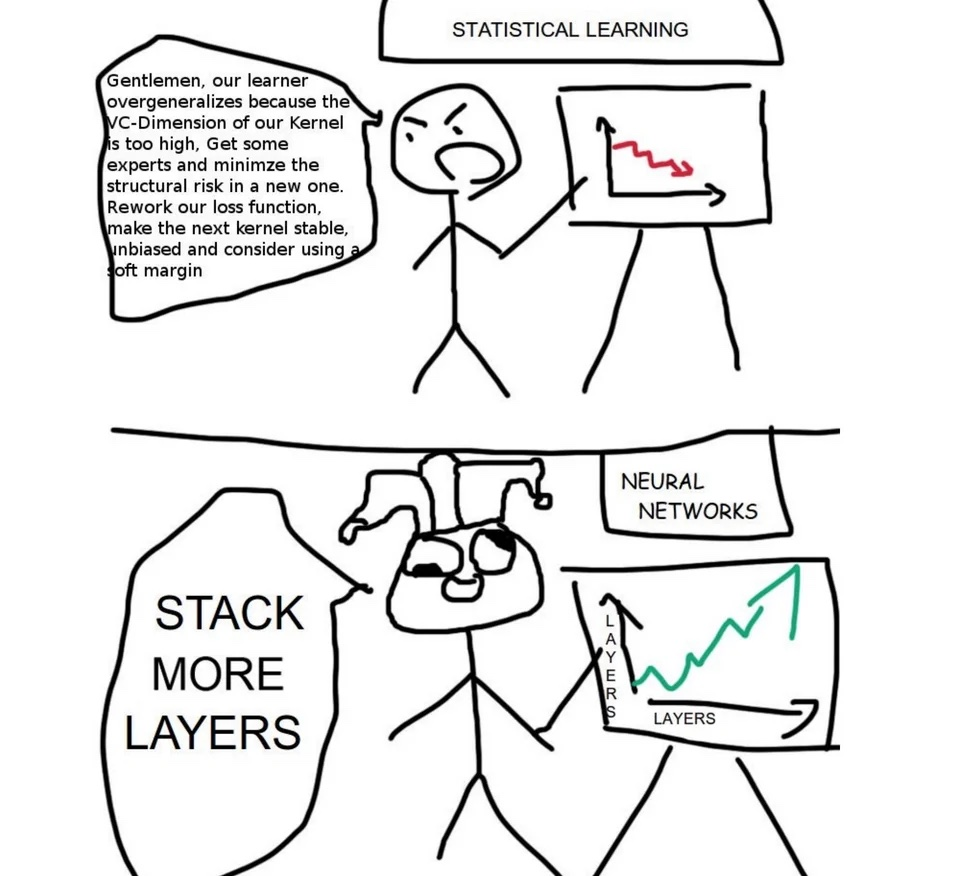
\includegraphics[width=\textwidth]{figures/intro/stackmoar.jpg}
\caption{
A caricature \citep{deleted_user_stack_2018} that summarises the opposing epistemic stances of the symbolic/connectionist divide at a glance. For those unfamiliar, here is a recap. The symbolic side is synonymous with Good-old-fashioned-artificial-intelligence (GOFAI), research programme from the 70s to create general artificial intelligence. However, programming this explicitly turned out to be very hard because it was tantamount to systematising all of reasoning and knowledge \citep{}frameproblem, which is why GOFAI is sometimes described as knowledge-based. In the meantime connectionist methods -- today synonymous with Deep Learning \citep{} -- leapfrogged GOFAI, for reasons explored in more detail in Section \ref{}. What distinguished connectionism was a reliance on data and compute rather than explicit programming, so it is sometimes described as knowledge-lean. A bullish sentiment arose among connectionists that cranking the handle to increase the size of the computer and the amount of training data would suffice to eventually obtain general artificial intelligence \citep{anderson_end_2008}. Debates surrounding this position fall generally under the umbrella of the epistemology of Data Science \citep{pietsch_epistemology_2022,desai_epistemological_2022}. In the case of LLMs specifically, modern debates of the bullish sentiment are developing, often rapidly. For example, in a thorough survey of LLM capabilities, \citep{} warned against a fallacious conflation of linguistic and cognitive abilities, while observing several failure modes of GPT3 in cognitive domains. By the time the paper was published, those observations no longer held for GPT3's successor, ChatGPT \citep{}, which patched the failures with the introduction of reinforcement learning.
}
\end{figure}
 
Connectionism is winning, in the sense that the lion's share of AI research today is connectionist \citep{}. Moreover, hostility (or at least indifference) to symbolic approaches is a stance espoused by some of the leading lights of modern machine learning \citep{}. This stance is worth elaborating and steelmanning for pen-and-paper-people in the context of language. First, many linguistic phenomena are nebulous \citep{} -- the boundary of a simile is like that of a cloud, not sharp like the boundary of a billiard ball. Second, linguistic phenomena are complex, dynamic, and multifactorial: there are so many interacting mechanisms and forces in the production and comprehension of language that even if we do have crisp mathematical models for all the constituent processes we are still left with something computationally irreducible \citep{}. The latter term refers to a special kind of computational difficulty which is best understood by example. We have a closed-form mathematical expression to shortcut the computation of the evolution of a system of two point masses under gravity, but we have no such shortcut for the three-body problem; the best we can do is simulate the system's evolution, and the lesson is that even for very simple systems, it is possible that no amount of causal-mechanistic understanding will simplify compututational simulation. These two points together weakly characterise the kinds of problem domains where machine learning shines. It is just a fact that LLM outputs today conform to any sensible understanding of syntax, semantics, pragmatics, conversational implicature, and whatever else we have theorised. It is just a fact that they produce better poetry and humor than anything we could explicitly program according to our current understanding. It is also a fact that they will only get better from here.\\

So, as far as practical language applications are concerned, for a theory to be a nonstarter, it needs to bring something to the table. To borrow terms from concurrency, there is already plenty of liveness, what is needed is more safety; liveness is when the program does something good, and safety is a guarantee it won't do something bad. For example; there is ongoing work in integrating LLMs with stuctured databases for uses where facts and figures matter \citep{}; there is still a need for safeguards to prevent harmful outputs \citep{} and adversarial attacks like prompt injection \citep{}; while LLMs give a very convincing impression of reasoned thought, we would like to be sure if ever we decide to use such a machine for anything more than entertainment, like deciding on a medical course of treatment \citep{} or making decisions with financial consequences \citep{}. The good news is that symbolic-compositional theories are the right shape for safety concerns, because they can be picked apart and reasoned about \citep{}. It is clear however that symbolic-compositional approaches by themselves are nowhere near achieving the kind of liveness LLMs have. Therefore, the direction of progress is synthesis.\\

The core value proposition for synthesis is explainable AI, which operates in a manner we can analyse, and if appropriate, constrain. For this purpose, merely knowing \emph{what} a deep-learning model is thinking is not enough: solving symbol-grounding\footnote{As a contextual aside, I recount the following from \citep{}, which argues that symbol-grounding is solvable from data alone, and in the process surveys the front of the symbol-grounding problem in explainability: the issue of whether LLMs encode what words refer to and mean. On the account of \citep{bender_climbing_2020}, the performance of current LLMs is a form of Chinese Room \citep{searle_minds_1980} phenomenon, so no amount of linguistic competence can be evidence that LLMs solve the symbol-grounding problem -- e.g. knowing what words refer to and mean. However, the available evidence appears to suggest otherwise -- large models converge on word embeddings for geographical place names that are isomorphic to their physical locations \citep{}. Since we know that brain activity patterns encode words in a manner that facilitates analogical reasoning in an abstract conceptual space \citep{}, extrapolating the ability of LLMs to encode analogical representations would in the limit suggest that LLMs encode meanings in a way isomorphic to how we do -- at least for individual tokens.} alone is a necessary but insufficient component. For instance, merely knowing what the weights of subnetworks of an image classification model represent \citep{} does not meet our requirement of an understanding of the computations that manipulate those representations. Moreover, purely data-driven methods to control the computation may incur ethical costs \citep{}, to say nothing of the potential harm that may result from a poorly safeguarded model \citep{}. Add to this the ever-growing dirty laundry lists of AI models failing \citep{} in inhuman ways, and the task of incorporating compositionality -- a formal understanding of \emph{how} models learn and reason -- gains urgency.\\

The investigation of the common ground between symbolic-composition and connectionism takes on, I suggest, essentially two, dual forms. The first kind uses connectionist methods to simulate symbolic-composition. The second kind is the inverse, where connectionist architectures are organised and reasoned with by symbolic-compositional means. Some examples of the first include implementing data structures as operations on high-dimensional vectors, taking advantage of the idiosyncrasies of linear algebra in very high dimension \citep{}, or work that explores how the structure of word-embeddings in latent space encode semantic relationships between tokens \citep{}. Some examples of the second include reasoning about the capability of graph neural networks by identifying their underlying compositional structure \citep{}, or architectures explicitly designed to instantiate symbolic-compositional structures using neural nets as constituent parts, such as GANs \citep{} and gradient boosted decision trees \citep{}. The work in this thesis builds upon a research programme -- DisCoCat, elaborated in Section \ref{} -- which lies somewhere in the middle of the duality. It is, to the best of my knowledge, the only approach that explicitly incorporates mathematically rigourous compositional structures with data-driven learning methods from the ground up. Fortifying this bridge across the aisle requires a little give from both sides; I ask only that reader entertain some pretty string diagrams.

\newthought{\textbf{Objection:} Aren't string diagrams just graphs? We understand graphs well enough that if that were the solution we would have had it by now.}

Yes and no!\footnote{A deeper objection here is that diagrams do not look like serious mathematics. Later I will give ample space to show how they are serious, but the reasons behind this rather common prejudice are worth elaborating. This is the wound Bourbaki has inflicted. Nicolas Bourbaki is a pseudonym for a group of French mathematicians, who wrote a highly influential series of textbooks. It is difficult to overstate their influence. The group was founded in the aftermath of the First World War, around the task of writing a comprehensive and rigourous foundations of mathematics from the ground up. The immediate \emph{raison-d'\^{e}tre} for this project was that extant texts at the time were outdated, and the oral tradition and living history of mathematics in institutions of learning were decimated by the deaths of mathematicians at war. In a broader historical context \citep{}, Bourbaki was a reactionary response to the crisis in the foundations of mathematics at the beginning of the century, elicited by Russell's paradox. Accordingly, their aims were rationalist, totalitarian, and high-modernist \citep{}, favouring abstraction and disdaining visualisation, in line with their contemporary artistic and musical fashions. Consequently, Bourbaki's Definition-Proposition-Theorem style of mathematical exposition is an evolved form of Euclid's that eschews intuition and example, a format pretending at timelessness that requires years of initiation to effectively read and write, and remains \emph{de rigeur} for rigour today in dry mathematics textbooks. The deeper objection arises from the supposition that serious mathematics ought to look arcane and difficult, as most mathematics exposition after Bourbaki is. The reply is that it need not be so, and that it was not always so! The Bourbaki format places emphasis and prestige upon the deductive activity that goes into proving a theorem, displacing other aspects of mathematical activity such as constructions, algorithms, and taxonomisation \citep{}. These latter aspects are better suited for the nebulous subject matter of natural language, which not lend itself well to theorems, but is a happy muse for mathematical play.} This point is best communicated by a mathematical koan. Consider the following game between two players, you and me. There are 9 cards labelled 1 through 9 face up on the table. We take turns taking one of the cards. The winner is whoever first has three cards in hand that sum to 15, and the game is a draw if we have taken all the cards on the table and neither of us have three cards in hand that sum to 15. I will let you go first. Can you guarantee that you won't lose? Can you spell out a winning strategy? If you have never heard this story, give it an honest minute's thought before reading on.\\

The usual response is that you don't know a winning strategy. I claim that you probably do. I claim that even a child knows how to play adeptly. I'll even wager a drink that you have played this game before. The game is Tic-Tac-Toe, also known as Naughts-and-Crosses: it is possible to arrange the cards in a 3-by-3 magic square, such that every column, row, and diagonal sums to 15.\\

The lesson here is that choice of representations matter. In the mathematical context, representations matter because they generalise differently. On the surface, here is an example of two representations of the same platonic mathematical object. However, Tic-Tac-Toe is in the same family as Connect-4 or 5-in-a-row on an unbounded grid, while the game with numbered cards generalises to different variants of Nim. That they coincide in one instance is a fork in the path. In the same way, viewing string diagrams as "just graphs" is taking the wrong path, just as it would be a mistake to dismiss graphs as "just sets of vertices and edges". String diagrams are indeed "just" a special family of graphs, just as much as prime numbers are special integers and analytic functions are special functions. Throughout this thesis I will be re-presenting familiar and unfamiliar things in string diagrams, so I request the reader to remember the koan and keep an open mind.\\

In a broader context, representations matter for the sake of improved human-machine relations. These two representations are the same as far as a computer or a formal symbol-pusher is concerned, but they make world of difference to a human native of meatspace. We ought to swing the pendulum towards incorporating human-friendly representations in language models, so that we may audit those representations for explainability concerns. As it stands, there is something fundamentally inhuman and behavioural about treating the production of language as a string of words drawn from a probability distribution. In practice, this is what LLMs do. When \emph{you} use language, do you feel like a diceroll? Even if we grant that the latent space of a data-driven architecture is an analog for the space of internal mental states of a human user of language, how can we know whether the spaces are structurally analogous to the extent that human-machine partnership through the interface of natural language is safe? So here again is the possible solution: we can guarantee that the latent-space representation of the machine is built up in the same way we build up a mental representation when we read a book or watch a film. We sketch how to approach this in Section \ref{}.

\section{\textbf{Question:} How do string diagrams help us understand language better?}

Another way to deal with the devastating question of LLMs is to reject it, on the basis that understanding LLMs is completely different from understanding language, and language is worth understanding in its own right. To illustrate this point by a thought experiment, what would linguistics look like if it began today? LLMs would appear to us as oracles; wise, superhumanly capable at language, but inscrutable. Similarly, most people effortlessly use language without a formal understanding which they can express. So the fundamental mystery would remain unchanged. Understanding how an LLM works cannot help: to borrow a thought from \citep{}, suppose you knew the insides of a mechanical calculator by heart. Does that mean you \emph{understand} arithmetic? At best, obliquely: implementing a computer for ideal arithmetic means compromises; the calculator is full of inessentialities and tricks against the constraints of physics. You would not know where the tricks begin and the essence ends. Similarly, suppose you knew every line of code and every piece of data used to train an LLM; does that mean you understand how language works? How does one delineate what is essential to language, and what is accidental? So the value proposition to establish is how string diagrams come into the picture for the linguist who is (definitionally) concerned with understanding how language works. The answer in short is that linguists have failed to provide an adequate understanding of language at the most basic level, and that string diagrams make it simpler to express an adequate account. Let's give the practical reader one more objection before we elaborate the reply.

\newthought{\textbf{Objection:} If the better theory is one that gives better predictions, aren't many theories of language knocked out of the game by an LLM before they can even get started?}

Whether LLMs are even a theory of language is a best debatable. There are various criteria -- not all independent -- that are arguably necessary for something to qualify as an explanatory theory, and while LLMs satisfice (or even excel) at some, they fail at others. Empirical adequacy -- the ability of theory to account for the available empirical data and make good predictions about future observations -- is one such criterion \citep{}, and here LLMs excel. In constast to the idealised and partial nature of formal theories, the nature of LLMs is that they are trained on empirical data about language that captures the friction of the real world. So, in terms of raw predictive power, we should naturally expect the LLMs to have an advantage over principled theories. They are so good at empirical capture that to some degree they automatically satisfy the related criteria of coherence -- consistency with other established linguistic theories -- and scope -- the ability to capture a wide range of phenomena.\\

While empirical capture is necessary for explanatory theories, it is insufficient. We may belay the order to vacate linguistics departments when we consider the case study of models of the solar system. The Ptolemaic geocentric model of the solar system was more empirically precise than the heliocentric Copernican, even though the latter was "more correct" \citep{}. This was because Ptolemaic epicycles can overfit to approximate any observed trajectory of planets. It took until Einstein's relativity to explain the perihelion of mercury, which at last aligned theoretical understanding with empirical observation. But Newton's theory of gravity was undeniably worthwhile science, even if it was empirically outperformed by its contemporaries.\\

There are several criteria where the adequacy of LLMs is unclear or debatable. Fruitfulness is a sociological criterion for goodness of explanatory theories, in that they should generate new predictions and lead to further discoveries and research \citep{}. While they are certainly a potent catalyst for research in machine learning, it is unclear how they relate to the subject matter of linguistics. Whether they satisfy Popper's criterion of falsifiability is as of yet not determined, because it is not settled how to go about falsifying the linguistic predictions of LLMs, or even express what the content of a theory embodied by an LLM is. The closest examples to falsifiability that come to mind are tests of LLM fallibility for reasoning and compositional phenomena \citep{}, or their weakness to adversarial prompt-injections \citep{}, but these weaknesses do not shed light on their linguistic competence and "understanding" directly.\\

Now the disappointments. LLMs are far from simple, and simplicity (Occam's Razor) is an ancient criterion for the goodness of explanation. Moreover, they fail at providing explanatory mechanisms \citep{}, and they do not unify or subsume our prior understandings \citep{}. The first two points are unobjectionable, so I will briefly elaborate on unification and subsumption of prior understandings, borrowing a framework from cognitive neuroscience. A common methodology for investigating cognitive systems is Marr's 3 levels \citep{} (poorly named, since they are not hierarchical, but more like interacting domains.) Level 1 is the computational theory, an extensional perspective that concerns tasks and functions: at this level on asks what the contents and aims of a system are, to evaluate what the system is computing and why, respectively. Level 2 is representation and algorithm, an intensional perspective that concerns the representational format of the contents within the system, and the procedures by which they are manipulated to arrive at outcomes and outputs. Level 3 is hardware, which concerns the mechanical execution of the system, as gears in a mechanical calculutor or as values, reads, and writes in computer memory. To be fair, in the case of LLMs, we understand well the nature of computational theory level, at least in their current incarnation as next-token-predictors, which is a narrow and clear task. Furthermore, we understand the hardware level well, from the silicon going up through the ladder of abstraction to software libraries and the componentwise activity of neural nets. There is something deeply wrong about our understanding -- if we can call it that -- of level 2. We have working understandings of several aspects about this level. We know something about the nature of internal representations in neural nets both in terms of semantic encoding within weight distributions \citep{} and of token-embeddings in latent space \citep{}. We can explain how transformer models work in terms of attention mechanisms and lookback \citep{}, which serves as working understanding of the procedural aspect of LLMs. We also understand mathematically how it is that these models are trained using data to produce the outputs they do. The deep problem is that in spite of these understandings which should jointly cover all of level 2, we only obtain explanations at the wrong level of abstraction for the purposes we care about \citep{}. Level 2 is in a sense the important level to get right for the purposes of explainability, auditability, and extension, since it is at the level of representation and procedure that we can investigate internal structure and match levels of abstraction across domains. Since the three levels interact, the challenge is to slot in a story about level 2 that coheres with what we already know about levels 1 and 3. I claim that we can go about this challenge using string diagrams as a lingua franca for mathematical linguists and machines.

\newthought{\textbf{Reply:} String diagrams, and category theory more broadly, are a good metalanguage for formal linguistics.}

Set-theoretical foundations of mathematics are not well suited for complex and interacting moving parts. The chief drawback is that if you want to specify a function, you have to spell out how it behaves on the domain and codomain, which means spelling out what the innards of the domain and codomain are; to specify a set-theoretic model necessitates providing complete detail of how every part looks on the inside\footnote{This is a foundational, innate problem of set theory. Consider the case of the cartesian product of sets, one of the basic constructions. $A \times B$ is the "set of ordered pairs" $(a,b)$ of elements from the respective sets, but there are many ways of encoding that are equivalent in spirit but not in syntax; a sign that the syntax is a hindrance. What we really want of the product is the property that $(a,b) = (c,d)$ just when $a = c$ and $b = d$. Now here is a small sampling of different ways to encode an ordered pair. Kuratowski's definition is
\[A \times B := \bigg\{ \{\{a\},\{a,b\}\} \ | \ a \in A \ , \ b \in B \bigg\}\]
Which could have just as easily been:
\[A \times B := \bigg\{ \{a,\{a,b\}\} \ | \ a \in A \ , \ b \in B \bigg\}\]
And here is Wiener's definition:
\[A \times B := \bigg\{ \{\{a,\varnothing\},b\} \ | \ a \in A \ , \ b \in B \bigg\}\]}. As you may already know, this representation-dependency is a nightmare when dealing with a complex system: you have to specify all the implementation details from start to finish, bottom-up. This leads to at least three problems.
\begin{enumerate}
\item{
The sociological problem is that this makes things difficult to understand unless you have invested a lot of time into mathematics in general.
}
\item{
Interoperability is tricky. When a programmer wants to use a data structure or algorithm, they do not always write it from scratch or copy code from stackoverflow; they may use a library that provides them structures and methods they can call without worrying about how those structures and methods are implemented all the way down. However, if you building a complex theory by spelling out implementations set-theoretically from the start, incorporating a new module from elsewhere becomes difficult if that module has encoded things in sets differently. A lot of busywork goes into translating foundations of formalisms at an analogous level to machine code, which is time better spent building upwards and outwards. A computer scientist might say that some abstraction is needed, and being one, I say so.
}
\item{
Third, and related to the second, is that set-theory is not the native language for the vast majority of practical computation. Often in the design of complex theories, we do not care about how precisely representations are implemented, instead we only care about placing constraints or guarantees on the behaviour of interacting interactions -- that is, we care about operational semantics.
}
\end{enumerate}

The problems I have mentioned above are obstacles, and I hope to show that using applied category theory as a metalanguage may be a solution. A broad theme of this thesis is to illustrate the economy and reach of applied category theory for dealing with compositional phenomena. Our capacity for language is one of the oldest and sophisticated pieces of compositional technology, maybe even the foundation of compositional thought. So, linguists are veteran students of compositionality and modularity. How does syntax compose meaning? How do the constraints and affordances of language interact? The discipline embodies a encyclopaedic record of how compositionality works "in the field", just as botanists record flowers, early astronomers the planetary motions, or stamp collectors stamps. But a disparate collection of observations does not a theory make; we will inevitably wish to bring it all together. I show that we can progress towards this aim using formal diagrams that our visual cortexes have built-in rules to manipulate, and that allow us to work at the level of abstraction we choose, so that we may easily incorporate other modules and find implementations in a variety of settings.

To summarise the first value proposition, string diagrams are an aesthetic, intuitive, flexible, and rigourous metalanguage syntax that gives agency to the modeller by operating at a level of abstraction of their choice. This means that the same diagrams are a common syntactic foundation that can model linear and affine algebra \citep{}, first order logic \citep{}, signal flow \citep{}, electrical circuits \citep{}, database operations \citep{}, spatial relations \citep{}, language games \citep{}, petri nets \citep{}, hypergraphs \citep{}, probability theory \citep{}, machine learning \citep{}, and quantum theory \citep{}, to name just a sample. In this vein, theories of syntax expressed in terms of string diagrams makes it easier to reason about expressive equivalence between theories at a compositional level. More precisely, a theory of syntax is expressed as a finitely presented symmetric monoidal category, and relationships between theories are expressed as symmetric monoidal functors, which are generalised structure-preserving maps. The upshot of reasoning in this way is that equivalences are established at a structural level between the atomic components of corresponding theories, which lets us do some crazy things.

\newthought{\textbf{TL;DR of introduction:} LLMs do not explain language, and formal linguists "explain" language using the mathematical equivalent of punchcard machines. Both sides have much to gain from synthesis, but synthesis requires a shared mathematical metalanguage. I propose string diagrams and applied category theory as a good candidate, and the rest of the thesis is about justifying the proposal.

\section{Synopsis of the thesis}

\marginnote{
\textbf{Novel contributions:}
\begin{itemize}
\item
Section \ref{} demonstrates how string-diagrammatic reasoning allows for graphical proofs of strong equivalences between typelogical, string-production, and further strong equivalence to a fragment of tree-adjoining grammars. 
\item
Text diagrams and text circuits lie at the heart of the above correspondences and of this thesis, which we introduce and investigate in Section \ref{} in an abridged re-presentation of \citep{}, culminating in a proof relating the expressive capacity of text circuits to a controlled fragment of English that serves as evidence that text circuits are a natural metalanguage for grammatical relationships that make no extraneous distinctions.
\item
In Section \ref{}, moving towards applications, I introduce the category of continuous relations, to set a mathematical stage upon which we can build toy models, expanding upon my previous work on linguistically compositional spatial relations \citep{} towards modelling mechanical systems and containers.
\item
I mathematically investigate the possibilities and limitations of textual modelling with text circuits on classical and quantum computers in Section \ref{} by examining the limitations of cartesian monoidal categories for modelling text circuits, taking the universal approximation theorem into account.
\item
In Section \ref{}, I extend the string-diagrammatic techniques used to prove correspondences between different syntactic theories to text circuits provides a framework for the formal, conceptually-compliant modelling of textual metaphor.
\item
I demonstrate a formal connection between tame topologies and tensed language in Section \ref{}, which extends to a formal framework to model narratives as database rewrites in Section \ref{}.
\end{itemize}
}

Chapter 2 provides the relevant background and foundations for category theory, machine learning, and formal syntax for this thesis, which lives at the intersection. The ideas required from the parent fields will be basic, so the exposition is meant to get readers across disciplines on the same page, not impress experts. For string diagrams I will first provide a primer for how process-theoretic reasoning with string diagrams work, by example. On the category theoretic end, I will recount symmetric monoidal categories as the mathematical objects that string diagrams are syntax for, as well as provide a working understanding of PROPs \citep{} and n-categories as formalised by \citep{}, which provide a metalanguage for specifying families of string diagrams. Once the reader is happy with string diagrams, for machine learning I will just introduce how deep neural nets and backpropagation work in string-diagrammatic terms to provide a foundation of formal understanding, and I will explain the mathematical and real-world reasons why deep learning is so powerful. For formal linguistics, I will sketch out a partial history of categorial linguistics in general, along the way briefly recasting \citep{} in more modern mathematical terminology to justify string diagrams as a generalisation of Montague's original conception of syntax and semantics.\\

Chapter 3 is about string diagrams for formal syntax. Here I recount context-free, pregroup, and tree-adjoining grammars to the reader, recast them string-diagrammatically, and relate them by means of discrete monoidal fibrations, a piece of mathematics I will develop. Then we (re)introduce text circuits as the common structure between those different theories of grammar that abstracts away differences in linear syntactic presentation while conserving a core set of grammatical relations. During my DPhil, I wrote a paper \citep{} in collaboration with Jonathon Liu and Bob Coecke which introduced text circuits in a pedestrian way, and characterised their expressive capacity with respect to a controlled fragment of English. I will just recover the main beats of that paper, this time using the metalanguage of n-categories.\\

Chapter 4 sets a mathematical stage for us to model and calculate using text circuits, for which purpose I introduce the category of continuous relations \textbf{ContRel}, a na\"{i}ve generalisation of the category of continuous maps between topological spaces. \textbf{ContRel} is new, in the sense that the category-theoretically obvious approaches to obtaining such a category either do not work or yield something different. This section culminates in formal semantics for topological concepts such as \texttt{inside} which underpin the kinds of schematic doodle cartoons we might draw on paper to illustrate events occurring in space.\\

Chapter 5 is a formal invitation to playtime for the reader who gets that far. I don't expect that I've explored any novel linguistic phenomena, and I don't think I've invented any substantially new mathematics. All I've done is a form of intellectual arbitrage, putting tools from one field to work in another. To properly give weight to my claim that string diagrams and category theory are a good metalanguage for linguistics as a whole, it is necessary to demonstrate breadth. So, I model linguistic topological concepts; I give a mathematical setting for the study of generalised anaphora that reference any meaningful part of text; I provide formal semantics for the container metaphor in particular and textual metaphors in general; I sketch a formal correspondence between tensed language and tame topologies that extends to formally reckoning with narrative structure. All of this is to show that the methods I use are flexible and not doctrinal. I am not interested in whether these topics have been mathematicised more thoroughly and deeply before; what I care to demonstrate is that a little category theory and some imagination can go a long way.\\

Finally, I close with a discussion and prospectus. For the convenience of the reader, bibliographies are placed at the end of each chapter. Corrections, comments, and suggestions are welcome at \texttt{vincentwangsemailaddress@gmail.com}. I hope you enjoy the read, or if nothing else, I hope you like my diagrams!

\bibliographystyle{plain}
\bibliography{thesis_intro}

\chapter{Background}\label{chapter:stringdiagrams}
\clearpage
\section{A Partial History of String Diagrams}

\newthought{We have always tried to capture language in diagrams.}\\
Every so often, someone tries once again to draw the shape of language.\\
...\\
Now it's our turn.\\
The difference this time is formality; we are using \emph{string diagrams}.

\newthought{String diagrams are formal reasoning and representation systems for monoidal categories.} Chronologically, those adjectives occurred in this order: 1) visual representation, 2) visual reasoning, 3) formal.

\subsection{Pre-formal Diagrams}

Pre-formal diagrams are about visual expression. By the restrictions of writing technologies, the kind of visual representations we are interested in are two-dimensional. So visual means geometric in the plane. The ancient ancestors of modern string diagrams are systems for visual representation alone. For these ancestral diagrams, reasoning, if there is any, takes place `elsewhere', not within and between diagrams.\\

Euclid: Geometry

Venn \& Carroll: Syllogisms

Petri: Chemistry

\subsection{Convergent Evolution}

String diagrams arise naturally as diagrammatic representations for formal theories where reoccurring variables or bookkeeping indices for keep track of pairwise connections become too unwieldy for one-dimensional syntax.

\newthought{In Physics}

\newthought{In Logic}

\newthought{In Computer Science}


\clearpage
\section{Process Theories}

This section seeks to give an introduction to process theories in an intuitively grounded manner. We aim here to build the process-theoretic mathematics towards linguistic spatial relations -- words like "to the left of" and "between" -- which are a common ground of competence we all possess. Here we only focus on geometric relations in two dimensional Euclidean space equipped with notions of metric and distance. This section provides adequate foundations to follow \citep{}talkspace, in which I demonstrate how text circuits can be obtained from sentences and how such text circuits interpreted in the category of sets and relations \textbf{Rel} provides a semantics for such sentences. Moreover, this section motivates the question of how to express the (arguably more primitive \citep{}piaget) linguistic topological concepts -- such as "touching" and "inside" -- the mathematics of which will be in Chapter \ref{}; the reader may skip straight to that chapter after this section if they are uninterested in syntax. We close this section with a brief aside on how process theories relate to mathematical foundations and computer science.

A \emph{process} is something that transforms some number of input system types to some number of output system types. We depict systems as wires, labelled with their type, and processes as boxes. We read processes from left to right.
\[\tikzfig{proctheory/process}\]
Processes may compose in parallel, which we depict as vertically stacking boxes.
\[\tikzfig{proctheory/processpar}\]
Processes may compose sequentially, which we depict as connecting wires of the same type from left to right.
\[\tikzfig{proctheory/processseq}\]
In these diagrams only input-output connectivity matters: so we may twist wires and slide boxes along wires to obtain different diagrams that still refer to the same process. So the diagram below is equal to the diagram above.
\[\tikzfig{proctheory/processeq}\]
Some processes have no inputs; we call these \emph{states}. 
\[\tikzfig{proctheory/state}\]
Some processes have no outputs; we call these \emph{tests}.
\[\tikzfig{proctheory/test}\]
A process with no inputs and no outputs is a \emph{number}; the number tells us the outcome of applying tests to a composite of states modified by processes.
\[\tikzfig{proctheory/number}\]

A process theory is given by the following data\footnote{Formally, process theories are symmetric monoidal categories []; see section \ref{}.}:
\begin{itemize}
    \item A collection of systems
    \item A collection of processes along with their input and output systems
    \item A methodology to compose systems and processes sequentially and in parallel, and a specification of the unit of parallel composition.
    \item A collection of equations between composite processes
\end{itemize}

\begin{example}[Linear maps with direct sum]
Systems are finite-dimensional vector spaces over $\mathbb{R}$. Processes are linear maps, expressed as matrices with entries in $\mathbb{R}$.\\
Sequential composition is matrix multiplication. Parallel composition of systems is the direct sum of vector spaces $\oplus$. The parallel composition of matrices $\mathbf{A}, \mathbf{B}$ is the block-diagonal matrix
$$\begin{bmatrix}
\mathbf{A} & \mathbf{0} \\
\mathbf{0} & \mathbf{B}
\end{bmatrix}$$
The unit of parallel composition is the singleton 0-dimensional vector space.
States are row vectors. Tests are column vectors. The numbers are $\mathbb{R}$.\footnote{Usually the monoidal product is written with the symbol $\otimes$, which denotes hadamard product for linear maps. The process theory we have just described takes the direct sum $\oplus$ to be the monoidal product. To avoid confusion we will use the linear algebraic notation when linear algebra is concerned.}
\end{example}

\begin{example}[Sets and functions with cartesian product]
Systems are sets $A,B$. Processes are functions between sets $f: A \rightarrow B$. Sequential composition is function composition. Parallel composition of systems is the cartesian product of sets: the set of ordered pairs of two sets.
\[A \otimes B = A \times B := \{(a,b) \ | \ a \in A, b \in B\}\]
The parallel composition $f \otimes g : A \times C \rightarrow B \times D$ of functions $f: A \rightarrow B$ and $g: C \rightarrow D$ is defined:
\[f \otimes g := (a,c) \mapsto (f(a),g(c))\]
The unit of parallel composition is the\footnote{There are many singletons, but this presents no problem for the later formal definition because they are all equivalent up to unique isomorphism.} singleton set $\{\star\}$. States of a set $A$ correspond to elements $a \in A$\footnote{We forgo the usual categorical definition of points from the terminal object in favour of generalised points from the monoidal perspective.}. Every system $A$ has only one test $a \mapsto \star$\footnote{This is since the singleton is terminal in \textbf{Set}.}. There is only one number.
\end{example}

\begin{example}[Sets and relations with cartesian product]
Systems are sets $A,B$. Processes are relations between sets $\Phi \subseteq A \times B$, which we may write in either direction $\Phi^*: A \nrightarrow B$ or $\Phi_*: B \nrightarrow A$.\footnote{Relations between sets are equivalently matrices with entries from the boolean semiring. Relation composition is matrix multiplication with the boolean semiring. $\Phi^*,\Phi_*$ are the transposes of one another.}
Sequential composition is relation composition:
\[A \overset{\Phi}{\nrightarrow} B \overset{\Psi}{\nrightarrow} C := \{(a,c) \ | \  a \in A, \ c \in C, \ \exists b_{\in B}: (a,b) \in \Phi \wedge (b,c) \in \Psi  \}\]
Parallel composition of systems is the cartesian product of sets. The parallel composition of relations $A \otimes C \overset{\Phi \otimes \Psi}{\nrightarrow} B \otimes D$ of relations $A \overset{\Phi}{\nrightarrow} B$ and $C \overset{\Psi}{\nrightarrow} D$ is defined:
\[\Phi \otimes \Psi := \{\big( (a,c) , (b,d) \big) \ | \ (a,b) \in \Phi \wedge (c,d) \in \Psi\}\]
The unit of parallel composition is the singleton. States of a set $A$ are subsets of $A$. Tests of a set $A$ are also subsets of $A$.
\end{example}

\subsection{What does it mean to copy and delete?}

Now we discuss how we might define the properties and behaviour of processes by positing equations between diagrams. Let's begin simply with two intuitive processes \emph{copy} and \emph{delete}:
\[\tikzfig{proctheory/copydelete}\]

\begin{example}[Linear maps]
Consider a vector space $\mathbf{V}$, which we assume includes a choice of basis. The copy map is the rectangular matrix made of two identity matrices:
\[\Delta_\mathbf{V}: \mathbf{V} \rightarrow \mathbf{V} \oplus \mathbf{V} := \begin{bmatrix} \mathbf{1}_\mathbf{V} & \mathbf{1}_\mathbf{V} \end{bmatrix}\]
The delete map is the column vector of 1s:
\[\epsilon_\mathbf{V}: \mathbf{V} \rightarrow \mathbf{0} := \begin{bmatrix} 1 \\ \vdots \\ 1 \end{bmatrix}\]
\end{example}

\begin{example}[Sets and functions]
Consider a set $A$. The copy function is defined:
\[\Delta_A : A \rightarrow A \times A := a \mapsto (a,a)\]
The delete funtion is defined:
\[\epsilon_A : A \rightarrow \{\star\} := a \mapsto \star\]
\end{example}

\begin{example}[Sets and relations]\label{relcopy}
Consider a set $A$. The copy relation is defined:
\[\Delta_A : A \nrightarrow A \times A := \{\big(a , (a,a) \big) \ | \ a \in A\}\]
The delete relation is defined:
\[\epsilon_A : A \nrightarrow \{\star\} := \{(a,\star) \ | \ a \in A\}\]
\end{example}

We may verify that, no matter the concrete interpretation of the diagram in terms of linear maps, functions or relations copy and delete satisfy the equations in the margin:\marginnote[-10cm]{
Formally, the following equations characterise a cocommutative comonoid internal to a monoidal category.
\begin{equation}\label{cocom}
\scalebox{0.75}{\tikzfig{bestiary/basicrelations}}
\end{equation}
}

It is worth pausing here to think about how one might characterise the process of copying in words; it is challenging to do so for such an intuitive process. The diagrammatic equations in the margin, when translated into prose, provide an answer.
\begin{description}
\item[\textbf{Coassociativity}:] says there is no difference between copying copies.
\item[\textbf{Cocommutativity}:] says there is no difference between the outputs of a copy process.
\item[\textbf{Counitality}:] says that if a copy is made and one of the copies is deleted, the remaining copy is the same as the original.
\end{description}

Insofar as we think this is an acceptable characterisation of copying, rather than specify concretely what a copy and delete does for each system $X$ we encounter, we can instead posit that so long as we have processes $\Delta_X: X \otimes X \rightarrow X$ and $\epsilon_X: X \rightarrow I$ that obey all the equational constraints above, $\Delta_X$ and $\epsilon_X$ are as good as a copy and delete.

\marginnote{
\begin{example}[Not all states are copyable]\label{ex:copyablestate}
Call a state \emph{copyable} when it satisfies the following diagrammatic equation:
\[\tikzfig{proctheory/copyable}\]
In the process theory of sets and functions, all states are copyable. Not all states are copyable in the process theories of sets and relations and of linear maps. For example, consider the two element set $\mathbb{B} := \{0,1\}$, and let $\top : \{\star\} \nrightarrow \mathbb{B} := \{(\star,0),(\star,1)\} \simeq \{0,1\}$. Consider the composite of $\top$ with the copy relation:
\[\top;\Delta_{\mathbb{B}} := \{\big(\star,(0,0)\big),\big(\star,(1,1)\big)\} \simeq \{(0,0),(1,1)\}\]
This is a perfectly correlated bipartite state, and it is not equal to $\{0,1\} \times \{0,1\}$, so $\top$ is not copyable.
\end{example}
}
\marginnote{
\begin{remark}\label{ft:determinism}
The copyability of states is a special case of a more general form of interaction with the copy relation:
\[\scalebox{0.75}{\tikzfig{proctheory/copyablefunc}}\]
A cyan map that satisfies this equation is said to be a homomorphism with respect to the commutative comonoid. In the process theory of relations, those relations that satisfy this equation are precisely the functions; in other words, this diagrammatic equation expresses \emph{determinism}.
\end{remark}}

Here is an unexpected consequence. Suppose we insist that \emph{to copy} in principle also implies the ability to copy \emph{anything} -- arbitrary states. From Example \ref{ex:copyablestate} and Remark \ref{ft:determinism}, we know that this demand is incompatible with certain process theories. In particular, this demand would constrain a process theory of sets and relations to a subtheory of sets and functions. The moral here is that process theories are flexible enough to meet ontological needs. A classical computer scientist who works with perfectly copyable data and processes might demand universal copying along with Equations \ref{cocom}, whereas a quantum physicist who wishes to distinguish between copyable classical data and non-copyable quantum data might taxonomise copy and delete as a special case of a more generic quasi-copy and quasi-delete that only satisfies equations \ref{cocom}.\footnote{Quantum physicists \emph{do} do this; see Dodo: []}

\subsection{What is an update?}\label{ss:update}

In the previous section we have seen how we can start with concrete examples of copying in distinct process theories, and obtain a generic characterisation of copying by finding diagrammatic equations copying satisfies in each concrete case. In this section, we show how to go in the opposite direction: we start by positing diagrammatic equations that characterise the operational behaviour of a particular process -- such as \emph{updating} -- and it will turn out that any concrete process that satisfies the equational constraints we set out will \emph{by our own definition} be an update.\\

Perhaps the most familiar setting for an update is a database. In a database, an \bM entry\e often takes the form of pairs of \bB fields\e and \bO values\e. For example, where a database contains information about employees, a typical entry might look like:
\[\texttt{\bM < \bB\textbf{NAME}\e:\bO Jono Doe\e, \bB\textbf{AGE}\e:\bO 69\e, \bB\textbf{JOB}\e:\bO CONTENT CREATOR\e, \bB\textbf{SALARY}\e:\bO\$420\e, ... >\e}\]
There are all kinds of reasons one might wish to update the value of a field: Jono might legally change their name, a year might pass and Jono's age must be incremented, Jono might be promoted or demoted or get a raise and so on. It was the concern of database theorists to formalise and axiomatise the notion of updating the value of a field -- \emph{independently of the specific programming language implementation of a database} -- so that they had reasoning tools to ensure program correctness []. The problem is reducible to axiomatising a \emph{rewrite}: we can think of updating a value as first calculating the new value, then \emph{putting} the new value in place of the old. Since often the new value depends in some way on the old value, we also need a procedure to \emph{get} the current value.\\

That was a flash-prehistory of \emph{bidirectional transformations} []. Following the monoidal generalisation of lenses in [], a rewrite as we have described above is specified by system diagrammatic equations in the margin, each of which we introduce in prose.

\marginnote[-5cm]{
\begin{description}
\item[\textbf{PutPut}:] Putting in one value and then a second is the same as deleting the first value and just putting in the second.
\[\scalebox{0.5}{\tikzfig{proctheory/putputs}}\]
\item[\textbf{GetPut}:] Getting a value from a field and putting it back in is the same as not doing anything.
\[\scalebox{0.5}{\tikzfig{proctheory/getput}}\]
\item[\textbf{PutGet}:] Putting in a value and getting a value from the field is the same as first copying the value, putting in one copy and keeping the second.
\[\scalebox{0.5}{\tikzfig{proctheory/putget}}\]
\item[\textbf{GetGet}:] Getting a value from a field twice is the same as getting the value once and copying it.
\[\scalebox{0.5}{\tikzfig{proctheory/getget}}\]
\end{description}
}

These diagrammatic equations do two things. First, they completely specify what it means to get and put values in a field in an implementation independent manner; it doesn't matter whether database entries are encoded as bitstrings, qubits, slips or paper or anything else, what matters is the interaction of get and put. Second, the diagrammatic equations give us the right to call our processes \emph{get} and \emph{put} in the first place: we define what it means to get and put by outlining the mutual interactions of get, put, copy, and delete. These two points are worth condensing and rephrasing:
\[
\textbf{A \emph{kind of process} is determined by patterns of interaction with other kinds of processes.}
\]

Now we can diagrammatically depict the process of updating Jono's age, by \bB getting\e Jono's \bO age value\e from their \bM entry\e, incrementing it by 1, and \bB putting\e it back in.

\[\tikzfig{proctheory/incrementage}\]

\subsection{Spatial predicates}

The following simple inference is what we will try to capture process-theoretically:

\begin{itemize}
\item \texttt{Oxford is north of London}
\item \texttt{Vincent is in Oxford}
\item \texttt{Rocco is in London}
\end{itemize}

How might it follow that \texttt{Rocco is south of Vincent}?\\

One way we might approach such a problem computationally is to assign a global coordinate system, for instance interpreting `north' and `south' and `is in' using longitude and latitude. Another coordinate system we might use is a locally flat map of England. The fact that either coordinate system would work is a sign that there is a degree of implementation-independence.\\

This coordinate/implementation-independence is true of most spatial language: we specify locations only by relative positions to other landmarks or things in space, rather than by means of a coordinate system. This is necessarily so for the communication of spatial information between agents who may have very different reference frames.\\

So the process-theoretic modelling aim is to specify how relations between entities can be \emph{updated} and \emph{classified} without requiring individual spatial entities to intrinsically possess meaningful or determinate spatial location.\\

So far we have established how to update properties of individual entities. We can build on what we have so far by observing that a relation between two entities can be considered a property of the pair.

\[placeholder\]

Spatial relations obey certain compositional constraints, such as transitivity in the case of `north of':

\[placeholder\]

Or the equivalence between 'north of' and 'south of' up to swapping the order of arguments:

\[\]

There are other general constraints on spatial relations, such as order-independence: the order in which spatial relations are updated does not (at least for perfect reasoners) affect the resultant presentation. This is depicted diagrammatically as commuting gates:

\[placeholder\]

\subsection{Processes, Sets, Computers}

\newthought{\texttt{Objection:} But what are the \emph{things} that the processes operate on?}

This is a common objection from philosophers who want their ontologies tidy. The claim roughly goes that you can't really reason about processes without knowing the underlying objects that participate on those processes, and since set theory is the only way we know how to spell out objects intensionally in this way, we should stick to sets. In simpler terms, if we're drawing only functions as (black)-boxes in our diagrams, how will we know what they do to the elements of the underlying sets?\\

The short answer is that -- perhaps surprisingly -- reasoning process-theoretically is mathematically equivalent to reasoning about sets and elements for all practical purposes; it is as if whatever is going on \emph{out there} is indifferent to whether we describe using a language of only nouns or only verbs.\\

In the case of set theory, let's suppose that instead of encoding functions as sets, we treat functions as primitive, so that we have a process theory where wires are labelled with sets, and functions are process boxes that we draw. The problem we face now is that it is not immediately clear how we would access the elements of any set using only the diagrammatic language. The solution is the observation that the elements $\{x \ | \ X\}$ of a set $X$ are in bijective correspondence with the functions from a singleton into $X$: $\{ f(\star) \mapsto x \ | \ \{\star\} \overset{f}{\rightarrow} X $. In prose, for any element $x$ in a set $X$, we can find a function that behaves as a pointer to that element $\{\star\} \rightarrow X$. So the states we have been drawing, when interpreted in the category of sets and function, are precisely elements of the sets that label their output wires.\\

The full and formal answer will require the reader to see Section \ref{} which spells out the category theory underpinning process theories. The caveat here is that process theories work for all \emph{practical} purposes, so I make no promises about how diagrams work for the kind of set theories that deals with hierarchies of infinities that set theorists do. For other issues concerning for instance the set of all functions between two sets, that requires symmetric monoidal closure, for which there exist string-diagrammatic formalisms \citep{}.

\newthought{\texttt{Objection:} But if they're expressively the same, what's the point?}

The following rebuttal draws on Harold Abelson's introductory lecture to computer science \citep{} (in which string diagrams appear to introduce programs without being explicitly named as such).\\

There is a distinction between declarative and imperative knowledge. Declarative knowledge is \emph{knowing-that}, for example, 6 is the square root of 36, which we might write $6 = \sqrt{36}$. Imperative knowledge is \emph{knowing-how}, for example, to obtain the square root of a positive number, for instance, by Heron's iterative method: to obtain the square root of $Y$, make a guess $X$, and take the average of $X$ and $\frac{Y}{X}$ until your guess is good enough.\\

Computer science concerns imperative knowledge. An obstacle to the study of imperative knowledge is complexity, which computer scientists manage by black-box abstraction -- suppressing irrelevant details, so that for instance once a square root procedure is defined, the reasoner outside the system does not need to know whether the procedure inside is an iterative method by Heron or Newton, only that it works and has certain properties. These black-boxes can be then composed into larger processes and procedures within human cognitive load.\\

Abstraction also yields generality. For example, in the case of addition, it is not only numbers we may care to add, but perhaps vectors, or the waveforms of signals. So there is an abstract notion of addition which we concretely instantiate for different domains that share a common interface; we may decide for example that all binary operations that are commutative monoids are valid candidates for what it means to be an addition operation.\\

In this light, string diagrams are a natural metalanguage for the study of imperative knowledge; string diagrams in fact independently evolved within computer science from flowcharts describing processes. Process theories, which are equations or logical sentences about processes, allow us to reason declaratively about imperative knowledge. Moreover, string diagrams as syntactic objects can be interpreted in various concrete settings, so that the same diagram serves as the common interface for a process like addition, with compliant implementation details for each particular domain spelled out separately.\label{sec:proctheory}
\clearpage
\section{Defining String Diagrams}

\subsection{Symmetric Monoidal Categories}

\subsection{PROPs}

\subsection{1-object 4-categories}


\clearpage
\section{A brief diagrammatic introduction to Neural Nets}

For those unfamiliar, it is worth understanding the fundamentals of how neural nets work, which illuminates how they are able to transmute large amounts of input data into strong and "theory-free" [] performance at tasks. The ability to convert data (in which we are drowning), along with the universal approximation theorem, explain why data-driven learning methods have recently outperformed handcrafted rules-based approaches to artificial intelligence. I will focus only on the basic deep neural net -- so the reader is warned that the state of the art in terms of learning architectures is far more sophisticated, such as transformers [] used in large language models. There are only two important takeaways from this section. First is that the reader must understand why it is that data-driven learning methods outperform human axiomatising when dealing with complex problem domains, and are therefore (with the usual caveats of explainability) preferable. Second is an understanding of the statement of the universal approximation theorem, which will reappear in Section \ref{sec:learn}, where it will be of service in an attempt to introduce compositionality via interacting ensembles of neural nets.

\newthought{Neural nets arise from a toy model of biological neurons.} At a glance, biological neurons have many receptors and one output, and the neuron fires a signal out if its combined inputs exceed an activation threshold. As a simplification, McCulloch-Pitts neurons are a sum of $n$ inputs passed through an activation function $\sigma: \mathbf{R}^n \rightarrow \mathbf{R}$ that is permitted to be nonlinear, but traditionally monotone increasing and sigmoidal, which bounds the range of the function $\exists a_{\mathbb{R}} b_{\mathbb{R}} \forall x_{\mathbb{R}} : a \leq \sigma(x) \leq b$, and asks that $\sigma$ approaches the lower and upper bounds in the limit as $x$ goes to $-\infty$ and $\infty$ respectively. Using the diagrammatic calculus for linear algebra [] equipped with a nonlinear activation function -- all of which is interpretable in \textbf{TopRel}, we can immediately grasp a visual resemblance between the designs of nature and man:

\[placeholder\]

\newthought{The first use of neural nets was in application to the problem of machine vision.} These first, single-layer neural nets were called \emph{perceptrons}. Mimicking the neuronal organisation of the visual cortex, it was a sensible idea to stack these layers on top of one another [] -- these layers are the original reason for the word "deep" in "deep learning", but words change in meaning over time.

\[placeholder\]

\newthought{The modern ubiquity of neural nets is due to several factors.} First is Hinton's backpropagation algorithm [] (which may be obsolete when you are reading this by Hinton's forward-forward second salvo [].) Observe that even after one has decided on the shape of the neural net in terms of neuronal connectivity, there are still many degrees of freedom in the parameters of the activation functions, in particular their horizontal shift (bias) and vertical stretching (weights). Borrowing diagrammatic notation for parameters as orthogonal wires from [], we can depict the degrees of freedom for a single neuron like this:

\[placeholder\]

\newthought{There is a massive space of parameters to set for even a moderately sized neural net.} So how do we set the parameters in such a way that the neural net computes something useful? Backpropagation solves this problem by leveraging the shape of a neural net. There are many easily searchable resources that cover backpropagation for the interested reader, including category-theoretic ones []. The simple explanation goes like this. Let's just focus on the weight parameter of each neuron. By analogy each neuron is a shitty person, and their weight is how strongly they hold a binary opinion. A neural net by analogy is a shitty rigid hierachical society with voters in the back and decision makers in the front. As a simple example, Alice and Bob each make a recommendation to Claire based on what they receive as input.

\[placeholder\]

Suppose that Claire's decision is wrong. She revises her own opinion then meets with her confidantes. Alice's recommendation was faulty, so Claire blames her; as a narcissistic defense, the viciousness of the blame is proportional to how wrong Claire was. Alice revises her own opinion proportional how mean Claire is being, and then Alice goes to seek out her confidantes to perpetuate a vicious cycle of psychological violence. Bob on the other hand was right, Claire tells him this with sheepishness proportional to her error, and he starts gloating "I told you so!" with glee proportional to how much cleverer he feels than Claire. So Bob becomes slightly more entrenched in his opinion, and then he goes to seek out his confidantes to either congratulate or belittle them, again proportional to how right he was. When all of the blame and backpatting has backpropagated throughout society, all the shitty people have adjusted their opinions, and their shitty society will be less prone to making the same mistake again. In human terms, this process is repeated for all of recorded history or longer, and then you have a neural net that can recognise handwritten digits.

\[placeholder\]

All this process needs to get started is a lot of labelled pairs of data, input along with the desired output for that input. The formal terminology for the scenario above that converts data into performance is "training", which is a computationally intensive process when lots of data is involved for big neural nets. So the second factor of the ubiquity of neural nets is Moore's law and analogues, which have overseen exponential growth in computational power and digital data storage capacity. Neural nets convert data and compute power as fuel into practical applications, and we live in an era of increasingly plentiful data and compute. Hence, the bitter lesson []; clever theories are no match for stupid methods with lots of data and a big computer. But why the hell should any of this work in the first place? Surely there are limits to what neural nets can do. Now the third factor; Moore's law and the bitter lesson might be cheated, but the third factor is a law backed by mathematics.

\begin{theorem}[Universal Approximation Theorem]

\end{theorem}

\newthought{Any problem that can be encoded as a continuous transformation of lists of real numbers into other lists of real numbers is potential prey for a big enough neural net.} A little creative thought will show that many practical problems can be treated in this way. The litigious can easily spot problems in neural nets outside of this law. For example, to the best of our knowledge there is no known lower bound for how much data is required -- as a function of desired accuracy within a desired confidence -- for a neural net to learn its target, so for all we know, any big neural net could suddenly fail on an easy input instance for no good reason. The universal approximation theorem is a double-edged sword, and the side that cuts the holder is that for complex problems, the input data cannot span the whole problem domain, so there will be many neural nets that agree perfectly on the training data but will perform differently out-of-distribution -- this common phenomenon is called "overfitting". Moreover, a major component of explainability from the human perspective is having mental representations and rules for their manipulation, whereas it is in general very difficult to determine how or even whether the neural net has internal representations and rules for its inputs. This introduces an ethical criterion that most data-driven algorithms fail: it is not a big deal to be recommended a show we do not like or have a machine play a game more innovatively than a human could, but if the stakes are higher, such as operating a vehicle or on a patient, we would prefer safety guarantees predicated upon internal representations and rules that we can understand and negotiate in human terms. In Section \ref{sec:learn} we will try to blunt the painful edges by using the universal approximation theorem and overfitting to our advantage in search of compositional, explainable internal representations.
\clearpage
\section{\textcolor{red}{A brief history of formal linguistics from the categorial perspective}}\label{sec:linghist}

\newthought{Summary:} Logical Type Theory in mathematics had a twin sister Categorial Grammar in linguistics, born in the 30s to Ajdukiewicz, raised into the 50s by Bar-Hillel and Lambek. Montague brought formal semantics to the picture via the Lambda-Calculus in the 70s, around the time Category Theory was getting started. The Curry-Howard correspondence between types and logic became Curry-Howard-Lambek to include categories, thus relating the typed lambda-calculus, intuitionistic logic, and cartesian closed categories. Lambek and Moortgat evolved categorial grammar into typelogical grammar; the use of different proof systems as models of grammar, which in turn suggested semantic categories beyond the cartesian closed setting. Alternative semantics in the form of quantum computers were realised by Coecke and Lambek, who together added string diagrams to the correspondence via a \emph{literally} observed correspondence between quantum bell states and reductions in Pregroup Grammar. Sazradeh and Clark enter the collaboration, bringing in Firth's distributional semantics -- which had by the time become computationally practical as the basis of neural methods for word encoding -- to create DisCoCat; a \underline{Dis}tributional, \underline{Co}mpositional and \underline{Cat}egorial framework for language. Mirroring the developmental circumstances of Discourse Representation Theory (itself independently conceived by Kamp and Heim), Coecke suggested promoting DisCoCat as framework for sentences towards a circuit-shaped framework for text -- DisCoCirc. But there remained unanswered questions and ugly spots, and some poor sap had to work out the formal details and clean things up. That poor sap is me.

\subsection{Curry-Howard-Lambek}

\begin{table}[]
\begin{tabular}{ccc}
(Typed) Lambda-Calculus & Intuitionistic Logic & Cartesian Closed Categories  \\
 Types & Propositions & Categories  \\
 Curry & Howard & Lambek 
\end{tabular}
\end{table}

This correspondence means that you can use the lambda-calculus on any family of data organised as a cartesian closed category; this could be strings, or sets and functions, topological shapes with holes, neural nets and finite vectors. So one small benefit of the category-theoretic viewpoint is a formal underpinning for these mild extensions.\\

Describing the bigger benefit requires a bigger picture. 


and Lambek and Coecke fully integrated the picture with syntax and categories. So the linguist's trinity may look something like this:

\begin{table}[]
\begin{tabular}{ccc}
Computation & Syntax & Semantics \\
(Typed) Lambda-calculus & Combinatory Categorial Grammar & Cartesian Closed Categories \\
Montague & Ajdukiewicz & Lambek
\end{tabular}
\end{table}

Or this:

\begin{table}[]
\begin{tabular}{ccc}
Computation & Syntax & Semantics \\
(Typed) Lambda-calculus & Pregroup Grammar & Rigid Autonomous Monoidal Categories \\
Montague & Ajdukiewicz & Lambek
\end{tabular}
\end{table}

So here is the story today as far as a linguist may be concerned. We know that Curry-Howard-Lambek- correspondence generalises: if you poke Howard for a grammar that is expressively distinct from a CCG, the type-theory changes, so Lambek gives a different family of semantic categories with different internal logics, and Curry gives you a syntactic composition gadget that differs from the lambda-calculus.

\subsection{What did Montague consider grammar to be?}\label{sec:monty}

\newthought{Summary:} Montague considered grammars to be coloured operads; Montague's "algebras" are (multi-sorted) clones, which are in bijection with (multi-sorted) Lawvere Theories, which are equivalently coloured operads.

\newthought{Montague semantics/grammar as Montague envisioned it is largely contained in two papers} -- \emph{Universal Grammar} \cite{montague1970universal}, and \emph{The Proper Treatment of Quantifiers in English} \cite{montague1973proper} -- both written shortly before his murder in 1971. The methods employed were not \emph{mathematically} novel -- the lambda calculus had been around since [DATE], and Tarski and Carnap had been developing intensional higher-order logics since [] -- but for linguists who, by-and-large, only knew first order predicate logic, these methods were a tour-de-force that solved longstanding problems in formal semantics. Thus, Montague semantics has largely been in the care of linguists rather than mathematicians. This meant sparse opportunity for the ideas to `update' according to mainstream developments in mathematics.\\

\newthought{There is a natural division of Montague's approach into two structural components.} First, the notion of a structure-preserving map from syntax to semantics. Second, the use of a powerful and expressive logic for semantics. We acknowledge the importance of the latter for formal semantic engineering, but here we will focus on just the former. According to Partee [], a formal semanticist, advocate, and torch-bearer for Montague, the chief interest of Montague's approach (as far as his contemporary \emph{linguists} were concerned) lay in the following ideas:

\begin{enumerate}
\item{Take truth conditions to be the essential data of semantics.}
\item{
\begin{enumerate}
\item{Use lambdas to emulate the structure of syntax...}
\item{...in a typed system of intensional predicate logic, such that composition is function application.}
\end{enumerate}}
\end{enumerate}

I have split the second point to highlight the role of lambdas. This element was the crux of the Montagovian revolution: according to Janssen in a personal communication with Partee from 1994, lambdas were ``...the feature that made compositionality possible at all."

In Section 1 of \emph{Universal Grammar}, Montague's first paragraph establishes common notions of relation and function -- the latter he calls \emph{operation}, to distinguish the $n$-ary case from the unary case which he calls \emph{function}. This is all done with ordinals indexing lists of elements of an arbitrary but fixed set $A$, which leads later on to nested indices and redundancy by repeated mention of $A$. We will try to avoid these issues going forward by eliding some data where there is no confusion, following common modern practice.\\

Next, Montague introduces his notion of \emph{algebra} and \emph{homomorphism}. He separates the data of the carrier set and the generators from the \emph{polynomial operations} that generate the term algebra.

\marginnote{
\begin{defn}[Generating data of an Algebra]\label{algdata} 
Let $A$ be the carrier set, and $F_\gamma$ be a set of functions $A^k \rightarrow A$ for some $k \in \mathbb{N}$, indexed by $\gamma \in \Gamma$. Denoted $\langle A, F_\gamma \rangle_{\gamma \in \Gamma}$
\end{defn}

The following three data are taken to be common among Montague's algebras:

\begin{defn}[Identities]\label{ids} 
A family of operations populated, for all $n, m \in \mathbb{N}$, $n \leq m$, by an $m$-ary operation $I_{n,m}$, defined on all $m$-tuples as

$$I_{n,m}(a) = a_n$$

where $a_n$ is the $n^{\text{th}}$ entry of the $m$-tuple $a$.
\end{defn}


\begin{defn}[Constants]\label{constants}
For all elements of the carrier $x \in A$, and all $m \in \mathbb{N}$, a constant operation $C_{x,m}$ defined on all $m$-tuples $a$ as:
$$C_{x,m}(a) = x$$
\end{defn}

\begin{defn}[Composition]\label{comp}
Given an $n$-ary operation $G$, and $n$ instances of $m$-ary operations $H_{1 \leq i \leq n}$, define the composite $G(H_i)_{1 \leq i \leq n}$ to act on $m$-tuples $a$ by:

$$G(H_i)_{1 \leq i \leq n}(a) = G(H_i(a))_{1 \leq i \leq n}$$

\emph{N.B.} the $m$-tuple $a$ is copied $n$ times by the composition. Writing out the right hand side more explicitly:

$$G\bigg( \ \big( \ H_1(a) \ , \ H_2(a) \ , \ \ldots \ , \ H_n(a) \ \big) \  \bigg)$$
\end{defn}

\begin{defn}[Polynomial Operations]\label{polyop}
The polynomial operations over an algebra $\langle A, F_\gamma \rangle_{\gamma \in \Gamma}$ are defined to be smallest class $K$ containing all $F_{\gamma \in \Gamma}$, identities, constants, closed under composition.
\end{defn}

\begin{defn}[Homomorphism of Algebras]\label{homo}
$h$ is a homomorphism from $\langle A, F_\gamma \rangle_{\gamma \in \Gamma}$ \emph{into} $\langle B, G_\gamma \rangle_{\gamma \in \Delta}$ iff
\begin{enumerate}
    \item{$\Gamma = \Delta$ and $\forall \gamma : $}
    \item{}
\end{enumerate}
\end{defn}
}

Definition \ref{ids} is equivalent to asking for all projections. Definitions \ref{ids} and \ref{comp} together characterise Montagovian algebras as (concrete) clones []. 


These are (concrete) clones [] and their homomorphisms. In modern terms, (abstract) clones known to be in bijection with Lawvere theories [] ------- . 

\subsection{On Syntax}

In Section 2, Montague seeks to define a broad conception of `syntax', which he terms a \emph{disambiguated language}. This is a free clone with carrier set $A$, generating operations $F_\gamma$ indexed by $\gamma \in \Gamma$, along with extra decorating information:

\begin{enumerate}
\item{$(\delta \in) \Delta$ is an (indexing) set of syntactic categories (e.g.~\texttt{NP}, \texttt{V}, etc.). Montague calls this the \emph{set of category indices}. $X_\delta \subseteq A$ form the \emph{basic expressions} of type $\delta$ in the language.}
\item{a set $S$ assigns types among $\delta \in \Delta$ to the inputs and output of -- not necessarily all -- $F_\gamma$.}
\item{a special $\delta_0 \in \Delta$ is taken to be the type of declarative sentences.}
\end{enumerate}

This definition is already considerably progressive. Because there is no condition of disjointness upon the $X_\delta$ -- a view that permits consideration of the same word playing different syntactic roles -- (1) permits the same basic expression $x \in A$ to participate in multiple types $X_\delta \subseteq A$ ($\star$). (2) misses being a normal typing system on several counts. There is no condition requiring all $F_\gamma$ to be typed by $S$, and no condition restricting each $F_\gamma$ to appear at most once: this raises the possibilities that ($\dag$) some operations $F$ go untyped, or that ($\ddag$) some are typed multiply.

Taking a disambiguated language $\mathfrak{U}$ on a carrier set $A$, Montague defines a \emph{language} to be a pair $L := <\mathfrak{U}, R>$, where $R$ is a relation from a subset of the carrier $A$ to a set $\texttt{PE}_L$, the set of \emph{proper expressions} of the language $L$. An admirable purpose of $R$ appears to be to permit the modelling of \emph{syntactic ambiguity}, where multiple elements of the term algebra $\mathfrak{U}$ (corresponding to syntactic derivations) are related to the same `proper language expression'.

However, we see aspects where Montague would have benefited from a more modern mathematical perspective: it appears that his intent was to impose a system of types to constrain composition of operations, but the tools were not available for him. Montague addresses ($\dag$) obliquely, by defining $\texttt{ME}_L$ to be the image in $\texttt{PE}_L$ of $R$ of just those expressions among $A$ that are typed. Nothing appears to guard against ($\ddag$), which causes problems as Montague expresses structural constraints (in the modern view) in terms of constraints on the codomain of an interpreting functor (cf. Montague's notion of \emph{generating} syntactic categories). One consquence, in conjunction with $(\star)$, is that every multiply typed operation $F$ induces a boolean algebra where the typings are the generators and the operations are elementwise in the inputs and output. Worse problems occur, as Montague's clone definition include all projectors, and when defined separately from the typing structure, these projectors may be typed in a way that permits operations that arbitrarily change types, which appears to defeat the purpose. We doubt these artefacts are intentional, so we will interpret Montague assuming his intent was a type-system as we would recognise one today.

By an evident extension of [Prop 3.51] to the typed case, a \emph{disambiguated language} is a multi-sorted Lawvere theory without relations, where the sorts are generated from products of a pointed set $(\Delta, \delta_0 : 1 \rightarrow \Delta)$.
\clearpage


\chapter{String Diagrams for Text}\label{chapter:textcircuits}
\clearpage

\section{How do we communicate using language?}

\marginnote{There is a distinction between \emph{grammars of the speaker} -- which produce sentences -- and \emph{grammars of the listener} -- which deduce sentences. Viewed as mathematical processes, the two kinds of grammars go in opposite directions; speaking grammars (e.g. string-rewrite systems) start with some grammatical structure, and require informational input (e.g. which rule comes next) to produce lists of words -- sentences. Conversely, listening grammars (e.g. typelogical grammars) start with a sentence, and require informational input (e.g. grammatical typing and which proof rule to try next) to deduce or parse a grammatical structure. Since we can understand each other, these two types of grammar must enjoy a systematic correspondence, and if one believes that semantics is compositional according to syntax, then the correspondence must further explain how both speaking and listening grammars manipulate the same underlying semantic expression, whatever that may be. \textbf{I argue that cofunctors capture this correspondence.}}

\newthought{Speakers and listeners understand one another.} Obviously, natural language involves communication, which involves at minimum a speaker and a listener, or a producer and a parser. The fact that communication happens at all is an everyday miracle that any formal understanding of language must account for. The miracle remains so even if we cautiously hedge to exclude pragmatics and context and only encompass small and boring fragments of factual language like \texttt{Alice sees Bob quickly run to school}. At minimum, we should be able to model a single conversational turn, where a speaker produces a sentence, the listener parses it, and both agree on the semantics. Here is a sequence of diagram equations that demonstrates mathematically how the miracle works for two toy grammars, for the sentence \texttt{Alice sees Bob quickly run to school}. On the left we have a grammatical structure obtained from a context-free grammar, and we have equations from a discrete monoidal fibration all the way to the right, where we obtain a pregroup representation of the same sentence. Going from right to left recovers the correspondence in the other direction.

\[\resizebox{1.5\textwidth}{!}{\tikzfig{tree2gate/workedexample/bigexaltogether}}\]

\newthought{Here are some na\"{i}ve observations on the nature of speaking and listening.} Let's suppose that a speaker, Preube, wants to communicate a thought to Fondo. Preube and Fondo cooperate to achieve the miracle; Preube encodes his thoughts -- a structure that isn't a one-dimensional string of symbols -- into a one-dimensional string of symbols. And then Fondo does the reverse, turning a one-dimensional string of symbols into a thought-structure like that of Preube's. It may still be that Preube and Fondo have radically different internal conceptions of what \texttt{FLOWERS} or \texttt{GIVING} or \texttt{BEETLES IN BOXES} are, but that is alright: we only care that the \emph{interacting structure} of the thought-relations in each person's head are the same, not their specific representations.

\newthought{The nature of their challenge can be summarised as an asymmetry of information.} The speaker knows the structure of a thought and has to supply information or computation in the form of choices to turn that thought into text. The listener knows only the text, and must supply information or computation to deduce the thought behind it. By this perspective, language is a shared and cooperative strategy to solve this (de/en)coding interaction.

\newthought{Speakers choose.} The speaker Preube must supply decisions about phrasing a thought in the process of speaking it. At some point at the beginning of an utterance, Preube has a thought but has not yet decided how to say it. Finding a particular phrasing requires choices to be made, because there are many ways to express even simple relational thoughts. For example, the relational content of our running example might be expressed in at least two ways (glossing over determiners):

\[\texttt{Alice likes flowers that Bob gives Claire.}\]
\[\texttt{Bob gives Claire flowers. Alice likes (those) flowers.}\]

Whether those decisions are made by committee or coinflips, they represent information that must be supplied to Preube in the process of producing language. For this reason, we consider context-free-grammars (and more generally, other string-rewrite systems) to be \emph{grammars of the speaker}, or \emph{productive grammars}. The start symbol $S$ is incrementally expanded and determined by rule-applications that are selected by the speaker. The important aspect here is that the speaker has an initial state of information $S$ that requires more information as input in order to arrive at the final sentence. Note that the concept of productive grammars are not exhausted by string-rewrite systems, merely that string-rewrite systems are a prototype that illustrate the concept well.

\newthought{Listeners deduce.} The listener Fondo must supply decisions about which words are grammatically related, and how. Like right-of-way in driving, sometimes these decisions are settled by convention, for example, subject-verb-object order in English. Sometimes sophisticated decisions need to be made that override or are orthogonal to conventions, as will be illustrated in the closing discussions and limitations section of this chapter. Since Fondo has to supply information in the form of choices in the process of converting text into meaning, we consider \emph{parsing grammars} -- such as all typelogical grammars, including pregroups and CCGs -- to be \emph{grammars of the listener}.

%As is convention for parsing, let's grant that there's a daemon in Fondo's head that makes all these lexical disambiguation choices for them, automatically settling on which sense of \texttt{the old man} or \texttt{somebody} is appropriate. As mathematicians looking for a toy model to get started, we are looking for the simplest kind of choice that Fondo can be trusted to make with only grammatical information available to them.

\newthought{The speaker's choices and the listener's deductions must be related.} The way the speaker decomposes the thought into words in text in the speaker's grammar must allow the listener to reconstruct the thought in the listener's grammar. Even in simple cases where both parties are aiming for unambiguous communication, the listener still must make choices. This is best illustrated by introducing two toy grammars -- we pick a context-free grammar for the speaker and a pregroup grammar for the listener, because they are simple, planar, and known to be weakly equivalent.

\begin{figure}[h!]\label{fig:GFOLex}
\centering
\[\resizebox{\textwidth}{!}{\tikzfig{intro/GFOLex}}\]
\caption{Preube and Fondo agree on the conceptual organisation entities and relations up to the words for those entities and relations. Just as a running example that does not affect the point, let's say we can gloss a thought in first order logic as $\exists a \exists b \exists c \exists f : A(a) \wedge B(b) \wedge C(c) \wedge F(f) \wedge L(a,f) \wedge G(b,c,f)$. In diagrammatic first order logic [], this is equivalently presented as the following diagrams (and any other diagram that agrees up to connectivity.) For example, Preube could ask Fondo comprehension questions such as \texttt{WHO GAVE WHAT? TO WHO?}, and if Fondo can always correctly answer -- e.g. \texttt{BOB GAVE FLOWERS. TO CLAIRE.} -- then both Preube and Fondo agree on the relational structure of the communicated thought to the extent permitted by language.}
\end{figure}

We assume Preube and Fondo speak the same language, so both know how words in their language correspond to putative building blocks of thoughts, and how the order of words in sentences and special grammatical words affect the (de-/re-)construction procedures. Now we have to explain how it is that the two can do this for infinitely many thoughts, and new thoughts never encountered before. Using string diagrams, this is surprisingly easy, because string diagrams are algebraic expressions that are invariant under certain topological manipulations that make it easy to convert between different shapes of language.

\begin{example}[\texttt{Alice likes flowers that Bob gives Claire.}] Let's say Preube is using a context-free grammar to produce sentences, and Fondo a pregroup grammar. \\

\begin{figure}[h!]\label{fig:GFOLex2a}
\centering
\[\resizebox{\textwidth}{!}{\tikzfig{intro/GFOLex2a}}\]
\caption{The rule of the game is that Preube and Fondo can agree on a string-diagrammatic encoding strategy before having to communicate with each other. Here is one such strategy. Preube might generate the example sentence as depicted.}
\end{figure}

\begin{figure}[h!]\label{fig:GFOLex2b}
\centering
\[\resizebox{\textwidth}{!}{\tikzfig{intro/GFOLex2b}}\]
\caption{Mathematically, it makes no difference if we take the Poincar\'{e} dual of the tree, so that zero-dimensional nodes become one-dimensional wires, and branchings become zero-dimensional points linking wires -- but we can just as well depict those points as boxes to label them more clearly.}
\end{figure}

\begin{figure}[h!]\label{fig:GFOLex2c}
\centering
\[\resizebox{\textwidth}{!}{\tikzfig{intro/GFOLex2c}}\]
\caption{Now that Preube can express their grammatical structure string-diagrammatically, they can try to deform their first-order-logic diagram -- representing what they mean to communicate -- subject to the constraint that every one of their branchings (the structure of the CFG) is something recoverable by Fondo using just pregroup reductions. To do so, Preube introduces a formal blue wire to mimic Fondo's sentence-type, and stuffs some complexity inside the labels in the form of internal wirings: a multiwire configuration for \texttt{that}, and a twist for \texttt{gives}. Those internal wirings are the content of Preube and Fondo's shared strategy.}
\end{figure}

\begin{figure}[h!]\label{fig:GFOLex2d}
\centering
\[\resizebox{\textwidth}{!}{\tikzfig{intro/GFOLex2d}}\]
\caption{So, when Fondo receives the sentence, Fondo's pregroup derivation yields a pregroup diagram that is connectively equivalent to what Preube stuffed inside the context-free grammar structure. So now the two have strong equivalence between their grammars in the sense that every one of Preube's branches is resolved by one of Fondo's reductions.}
\end{figure}

\begin{figure}[h!]\label{fig:GFOLex2}
\centering
\[\resizebox{\textwidth}{!}{\tikzfig{intro/GFOLex2}}\]
\caption{Now to fully recover Preube's intended FOL-diagram, Fondo refers to the internal wirings that form their shared strategy, and fills those in.}
\end{figure}
\end{example}
\clearpage

\begin{example}[\texttt{Bob gives Claire flowers. Alice likes flowers.}] Now we try the same content as the previous example but presented as a text with two sentences.
\begin{figure}[h!]\label{fig:GFOLex3a}
\centering
\[\resizebox{\textwidth}{!}{\tikzfig{intro/GFOLex3a}}\]
\caption{Preube's diagram morphed to fit a text circuit. The dotted blue line is a formal mark to indicate a sentential boundary. Observe how new discourse elements are introduced as states, and how open wires correspond to ongoing discourse and deletions mark completed discourse. This diagram also indicates that text circuits can be given semantics in FOL.}
\end{figure}

\begin{figure}[h!]\label{fig:GFOLex3a}
\centering
\[\resizebox{\textwidth}{!}{\tikzfig{intro/GFOLex3b}}\]
\caption{Fondo already knows how to parse individual sentences to extract the FOL using internal wirings. Observe there is a mathematical complication that arises in determining how many noun-wires should go into the sentence wire-bundle; we need to account for this later.}
\end{figure}

\begin{figure}[h!]\label{fig:GFOLex3a}
\centering
\[\resizebox{\textwidth}{!}{\tikzfig{intro/GFOLex3}}\]
\caption{To deal with text, Fondo can pass a growing bundle of sentence wires along horizontally.}
\end{figure}
\end{example}

\subsection{Discrete Monoidal Fibrations}

To capture the kinds of diagrammatic correspondences we have just sketched, we will develop monoidal cofunctors diagrammatically. The first step is introducing the concept of a discrete monoidal fibration\footnote{Expressing the coherence conditions of monoidal functors using equations involving functor boxes as below is not new \bR CITE \e. The idea of a functor being simultaneously monoidal and a fibration is not new \bR CITE \e. What is new is minor: the express requirement that the lifts of the fibration satisfy interchange, which is in general not guaranteed by just having a functor be monoidal and a (even discrete) fibration [fosco].}
: a mathematical bookkeeping tool that relates kinds of choices speakers and listeners make when generating and parsing text respectively. This in turn will require introducing \emph{monoidal functor boxes}.

\begin{figure}[h!]\label{fig:outsidein}
\centering
\[\resizebox{0.75\textwidth}{!}{\tikzfig{tree2gate/conventions/outsidein}}\]
\caption{There are two conventions for depicting the action of a monoidal functor on parts of a string diagram. The first follows source-to-target \emph{outside-in}. This convention is used for work in internal wirings, since it is well-suited for describing functors that send atomic generators in their domain to more complex diagrams in their domain.}
\end{figure}

\begin{figure}[h!]\label{fig:insideout}
\centering
\[\resizebox{0.75\textwidth}{!}{\tikzfig{tree2gate/conventions/insideout}}\]
\caption{The other convention, following \bR CITE \e, is \emph{inside-out}. For the following section, we will define the coherence conditions of discrete monoidal fibrations using this convention.}
\end{figure}

\begin{figure}[h!]
\[\resizebox{0.5\textwidth}{!}{\tikzfig{tree2gate/mfunctorbox/mfbox-notation}}\]
\caption{Suppose we have a functor between monoidal categories $\mathbf{F}: \mathcal{C} \rightarrow \mathcal{D}$. Then we have this diagrammatic representation of a morphism $\mathbf{F}A \overset{\mathbf{F}f}{\rightarrow} \mathbf{F}B$ in $\mathcal{D}$.}
\end{figure}

\begin{figure}[h!]
\[\resizebox{0.5\textwidth}{!}{\tikzfig{tree2gate/mfunctorbox/mfbox-seq}}\]
\caption{The use of a functor box is like a window from the target category $\mathcal{D}$ into the source category $\mathcal{C}$; when we know that a morphism in $\mathcal{D}$ is the image under $\mathbf{F}$ of some morphism in $\mathcal{C}$, the functor box notation is just a way of presenting all of that data at once. Since $\mathbf{F}$ is a functor, we must have that $\mathbf{F}f ; \mathbf{F}g = \mathbf{F}(f;g)$. Diagrammatically this equation is represented by freely splitting and merging functor boxes vertically.}
\end{figure}

\begin{figure}[h!]
\[\resizebox{0.5\textwidth}{!}{\tikzfig{tree2gate/mfunctorbox/mfbox-fibration+structural}}\]
\caption{Assume that $\mathbf{F}$ is strict monoidal; without loss of generality by the strictification theorem \bR CITE \e, this lets us gloss over the associators and unitors. For $\mathbf{F}$ to be strict monoidal, it has to preserve monoidal units and tensor products on the nose: i.e. $\mathbf{F}I_\mathcal{C} = I_\mathcal{D}$ and $\mathbf{F}A \otimes_\mathcal{D} \mathbf{F}B = \mathbf{F}(A \otimes_\mathcal{C} B)$. Diagrammatically these structural constraints amount to these equations.}
\end{figure}

\begin{figure}[h!]
\[\resizebox{0.5\textwidth}{!}{\tikzfig{tree2gate/mfunctorbox/mfbox-tensor}}\]
\caption{What remains is the monoidality of $\mathbf{F}$, which is the requirement $\mathbf{F}f \otimes \mathbf{F}g = \mathbf{F}(f \otimes g)$. Diagrammatically, this equation is represented by freely splitting and merging functor boxes horizontally; analogously to how splitting vertically is the functor-boxes' way of respecting sequential composition, splitting horizontally is how they respect parallel composition.}
\end{figure}

\begin{figure}[h!]
\[\resizebox{\textwidth}{!}{\tikzfig{tree2gate/mfunctorbox/mfbox-twist}}\]
\caption{And for when we want $\mathbf{F}$ to be a (strict) symmetric monoidal functor, we are just asking that boxes and twists do not get stuck on one another.}
\end{figure}

\begin{figure}[h!]
\[\resizebox{0.75\textwidth}{!}{\tikzfig{tree2gate/mfunctorbox/mfbox-prefibex}}\]
\caption{To motivate fibrations, first observe that by the diagrammatic equations of monoidal categories and functor boxes we have so far, we can always "slide out" the contents of a functor box out of the bottom. When can we do the reverse? That is, take a morphism in $\mathcal{D}$ and \emph{slide it into} a functor box? We know that in general this is not possible, because not all morphisms in $\mathcal{D}$ may be in the image of $\mathbf{F}$. So instead we ask "under what circumstances" can we do this for a functor $\mathbf{F}$? The answer is when $\mathbf{F}$ is a discrete fibration.}
\end{figure}

\begin{figure}[h!]
\[\resizebox{0.5\textwidth}{!}{\tikzfig{tree2gate/mfunctorbox/mfbox-fibration}}\]
\caption{
\begin{defn}[Discrete opfibration]
$\mathbf{F}: \mathcal{C} \rightarrow \mathcal{D}$ is a \emph{discrete fibration} when:
for all morphisms $f: \mathbf{F}A \rightarrow B$ in $\mathcal{D}$ with domain in the image of $\mathbf{F}$, there exists a unique object $\Phi^A_f$ and a unique morphism $\phi_f: A \rightarrow \Phi^A_f$ in $\mathcal{C}$, such that $f = \mathbf{F}\phi_f$. Diagrammatically, we can present all of the above as an equation reminiscent of sliding a morphism \emph{into} a functor box from below.
\end{defn}
}
\end{figure}


\begin{figure}
\[\resizebox{\textwidth}{!}{\tikzfig{tree2gate/mfunctorbox/mfbox-fibration+interchange}}\]
\caption{\begin{defn}[Monoidal discrete opfibration]
We consider $\mathbf{F}$ to be a \emph{(strict, symmetric) monoidal discrete opfibration} when it is a (strict, symmetric) monoidal functor, a discrete opfibration, and the depicted equations relating lifts to interchange hold. The diagrammatic motivation for the additional coherence equations is that -- if we view the lifts of opfibrations as sliding morphisms into functor boxes -- we do not want the order in which sliding occurs to affect the final result. In this way, lifts behave as 'graphical primitives' in the same manner as interchange isotopies and symmetry twists.
\end{defn}}
\end{figure}

\begin{figure}[h!]\label{fig:plan1}
\[\resizebox{0.75\textwidth}{!}{\tikzfig{tree2gate/workedexample/bigex012}}\]
\caption{We aim to be able to use discrete monoidal functor-boxes like so. In the leftmost diagram, we would like to graphically introduce pregroup states. In the first equation (isomorphism), we would like to use the monoidal condition of the functor to horizontally merge functor boxes. In the second equation, we would like to use the discrete fibration condition of the functor to expand the box downwards, converting a string diagram obtained from a context-free grammar into a pregroup diagram. Observe that the adverb \texttt{quickly} has its label vertically flipped, alongside the adposition \texttt{to} and the sentential-complement verb \texttt{sees}. This is by design for all grammatical categories where pregroup typings are contextually dependent, as will be illustrated in Figure \ref{fig:plan2}.}
\end{figure}

\begin{figure}[h!]\label{fig:plan2}
\[\resizebox{0.5\textwidth}{!}{\tikzfig{tree2gate/workedexample/gather_quickly}}\]
\caption{\texttt{quickly} could find itself modifying an intransitive (single noun) or transitive (two noun) verb. Suppose that it is the job of some process $\textcolor{orange}{\texttt{q'}}$ to handle intransitive verbs, and similarly $\textcolor{orange}{\texttt{q''}}$ to handle transitive ones. We use the functor for bookkeeping, by asking it to send both $\textcolor{orange}{\texttt{q'}}$ and $\textcolor{orange}{\texttt{q''}}$ to the dependent label $\textcolor{orange}{\bar{\texttt{q}}}$. Treating the label as a test rather than a state allows the fibration-box to choose the right version based on the domain wires as it expands top-down.
}
\end{figure}

\begin{figure}[h!]\label{fig:plan3}
\[\resizebox{0.5\textwidth}{!}{\tikzfig{tree2gate/workedexample/bigex_2bad}}\]
\caption{However, this procedure as described is at risk of being ill-defined. Observe that in the third diagram of Figure \ref{fig:plan1}, the assignment of wires in the domain of the functor to wires in the codomain of the functor is only declared by diagrammatic grouping; if we consider the algebraic data available in the third diagram, really all we have is the data in the figure. How do we know which wires in the domain of the functor correspond to which wires in the codomain? Resolving this issue is the purpose of the next section.}
\end{figure}

\clearpage

\subsection{Strictified diagrams for monoidal categories}

The crux of the issue sketched in Figure \ref{fig:plan3} is that while pregroup \emph{proofs} -- viewed as sequent trees -- syntactically distinguish the roots of subtrees, interpretation as pregroup \emph{diagrams} in a monoidal category forgets the subtree structure of the specific proof the diagram arises from. But it is precisely this forgotten structure that contains the algebraic data we require to keep track of (co)domain data diagrammatically. So a solution would be to force the diagrams in the blue domain recording pregroup data to hold onto this proof structure. For this purpose we use strictified diagrams for monoidal categories, defined in the margins.\\

\marginnote{
\begin{defn}[Strictified string diagrams]\label{defn:strict}
(Presentation taken from \bR CITE \e) Fix an arbitrary (non-strict) monoidal category $\mathcal{C}$. The \emph{strictification} $(\overline{\mathcal{C}},\bullet)$ is defined as follows (where strictness of $\overline{\mathcal{C}}$ entitles use of string-diagrammatic notation):
\begin{itemize}
\item[(1)]{Objects $\overline{A}$ for each $A \in \mathcal{C}$}
\end{itemize}
\end{defn}
}

\marginnote{
\begin{itemize}
\item[(2)] The following generators, with $\overline{f}: \overline{A} \rightarrow \overline{B}$ for each $f \in \mathcal{C}(A,B)$, where we adopt the convention of notating the monoidal unit with a dashed line:
\[\resizebox{\marginparwidth}{!}{\tikzfig{strictify/strictgens}}\]
\end{itemize}
}

\marginnote{
\begin{itemize}
\item[(3)] The following functoriality equations:
\[\resizebox{\marginparwidth}{!}{\tikzfig{strictify/strictfunct}}\]
\end{itemize}
}

\marginnote{
\begin{itemize}
\item[(4)] The following adapter equations:
\[\resizebox{\marginparwidth}{!}{\tikzfig{strictify/strictadapt}}\]
\end{itemize}
}

\marginnote{
\begin{itemize}
\item[(3)] The following representations of the natural isomorphisms in the definition of a monoidal category:
\[\resizebox{\marginparwidth}{!}{\tikzfig{strictify/strictators}}\]
\end{itemize}
}

\marginnote{
\begin{proposition}[$\bar{\mathcal{M}}$ and $\mathcal{M}$ are monoidally equivalent]

\begin{proof}
\bR CITE \e
\end{proof}
\end{proposition}
}

We are seeking some way to algebraically group or bracket together pregroup types that arise from a single word, in a distinguished way from concatenation-as-tensor. In this way we can preserve the structure of pregroup-sequent proofs: grouping indicates a node in the proof-tree, while tensor indicates parallel composition of proof trees. With strictified diagrams, we can model bracketing with biased tensor structure, e.g. treating for instance the left-nested tensoring $(\cdots((A \otimes B) \otimes C) \cdots \otimes \cdots Z)$ as a bracketed expression $[A \otimes B \cdots \otimes Z]$.

\begin{construction}[Pregroups with bracketing]\label{cons:bracketing}
Where $\mathcal{P}$ is a monoidal category generated by pregroup states and (directed) cups, we define pregroups-with-bracketing as subcategory of the \emph{free} strictification $\overline{\mathcal{P}}$, which consists of all the generators of the strictification $\overline{\mathcal{P}}$ as given by Definition \ref{defn:strict}, but none of the additional equations. The subcategory is constructed from the following generators:
\begin{itemize}
\item For each pregroup state $\texttt{w}: I \rightarrow \bigotimes\limits_{i} X_i$, a strictified state generator $\texttt{w}: I \rightarrow (\cdots((X_1 \otimes X_2) \otimes \cdots X_i) \cdots )$ with left-nested syntactic tensors. To illustrate, a state with 5 wires would correspond to a generator as follows:
\[\tikzfig{strictify/strictstate}\]
\item Let $[A \cdot B \cdots Z]$ denote the left-nested tensoring $((A \otimes B) \cdots \otimes Z)$, and let $\mathbf{X}$ denote $(\bigotimes\limits_i X_i)$. For each directed cap $\mathbf{X} \otimes \mathbf{X}^{-1} \rightarrow I$ (and symmetrically for caps of the other direction and cups), and for each pair of bracketed types $[\mathbf{A} \cdot \mathbf{X}]$ and $[\mathbf{X}^{-1} \cdot \mathbf{B}]$, we ask for a generator that fully detensors, applies the directed cup, and then retensors. Diagrammatically, this amounts to asking for generators that look like the following, that mimick a single proof step.
\[\tikzfig{strictify/stricteval}\]
\end{itemize}
\end{construction}

Construction \ref{cons:bracketing} solves the (co)domain assignment problem by organising the data as a monoidal cofunctor.

\clearpage
\subsection{Monoidal Cofunctors}

\marginnote{
These definitions and conventions follow \bR CITE \e. Given a (small) category $\mathcal{C}$ we notate the objects $\mathcal{C}_0$ and the morphisms $\mathcal{C}_1$, hence a functor $F: \mathcal{C} \rightarrow \mathcal{D}$ consists of an object assignment $F_0: \mathcal{C}_0 \rightarrow \mathcal{D}_0$ and a morphism assignment $F_1: \mathcal{C}_1 \rightarrow \mathcal{D}_1$.
}

\marginnote{
\begin{defn}[Cofunctors]
From \bR CITE Defn 2.2 \e.  A \emph{cofunctor} $(f,\varphi): \mathcal{C} \nrightarrow \mathcal{D}$ consists of a function $f: \mathcal{C}_0 \rightarrow \mathcal{D}_0$ which I'll call \emph{lowering}, together with a \emph{lifting operation} $\varphi$, a function that maps pairs of objects of $\mathcal{C}$ and certain morphisms in $\mathcal{D}$ to morphisms of $\mathcal{C}$:
\[(c \in \mathcal{C}_0, f(c) \overset{u}{\longrightarrow} b \in \mathcal{D}_1) \ \mapsto \ a \overset{\varphi(c,u)}{\longrightarrow} \mathtext{cod}(\varphi(c,u))\]
The following conditions are required:
\begin{enumerate}
\item Lowering the tip of a lifted arrow gets you back where you started.\[f(\mathtext{cod}(\varphi(c,u))) = b\]
\item The lifts of identities are identities.\[\varphi(c,1_{f(c)}) = 1_c\]
\item The lift of composites is the composite of lifts-with-respect-to the tips of lifted arrows.\[\varphi(c, v \circ u) = \varphi(\mathtext{cod}(\mathtext{cod}(\varphi(c,u))),v) \circ \varphi(c,u)\]
\end{enumerate}
\end{defn}
}

\marginnote{
\begin{remark}
Conditions 2 and 3 of the definition of cofunctor are reminiscent of functors. It is instructive but tedious to calculate with the base definition. Fortunately, there is a slick alternative, due to Clarke.
\end{remark}
}

\marginnote{
\begin{defn}[Bijective-on-objects functor]
From \bR CITE, Defn 2.8 \e. A functor $F: \mathcal{C} \rightarrow \mathcal{D}$ is \emph{bijective-on-objects} if for all $d \in \mathcal{D}$, there exists a $c \in \mathcal{C}$ such that $Fc = d$.
\end{defn}
}

\marginnote{
\begin{proposition}[Cofunctors as spans of functors]
From \bR CITE, Prop 2.10 \e, all cofunctors $(f,\varphi):\mathcal{C} \nrightarrow \mathcal{D}$ correspond to spans of functors where the left leg $L$ is bijective on objects and the right leg $R$ is a discrete opfibration:
% https://q.uiver.app/?q=WzAsMyxbMiwwLCJcXG1hdGhjYWx7WH0iXSxbMCwyLCJcXG1hdGhjYWx7Q30iXSxbNCwyLCJcXG1hdGhjYWx7RH0iXSxbMCwxLCJGIiwyLHsic3R5bGUiOnsidGFpbCI6eyJuYW1lIjoiaG9vayIsInNpZGUiOiJib3R0b20ifX19XSxbMCwyLCJHIiwwLHsic3R5bGUiOnsiaGVhZCI6eyJuYW1lIjoiZXBpIn19fV1d
\[\begin{tikzcd}[ampersand replacement=\&]
	\&\& {\Lambda(f,\varphi)} \\
	\\
	{\mathcal{C}} \&\&\&\& {\mathcal{D}}
	\arrow["L"', hook', from=1-3, to=3-1]
	\arrow["R", two heads, from=1-3, to=3-5]
\end{tikzcd}\]
Conversely, by \bR CITE, Prop 2.10 \e, for every span of functors where the left leg is bijective on objects and the right leg is a discrete opfibration,
\[\begin{tikzcd}[ampersand replacement=\&]
	\&\& {\mathcal{X}} \\
	\\
	{\mathcal{C}} \&\&\&\& {\mathcal{D}}
	\arrow["F"', hook', from=1-3, to=3-1]
	\arrow["G", two heads, from=1-3, to=3-5]
\end{tikzcd}\]
there exists a cofunctor $(f,\varphi):\mathcal{C} \nrightarrow \mathcal{D}$ and an isomorphism $J: \Lambda(f,\varphi) \rightarrow \mathcal{X}$ such that $FJ = L$ and $GJ = R$.
\end{proposition}
}

Pregroups by themselves are thin rigid autonomous categories, meaning there is at most one morphism between any pair of objects and that there are directed cups and caps in addition to plain monoidal structure. Thinness raises big issues for compositional semantics. Firstly, contra the aims of DisCoCat, all grammatically correct sentences correspond to states on the sentence type, which must all be equal by thinness, hence \emph{no functor} from the pregroup grammar to any other category can distinguish different sentences. One workaround to save claims of functoriality is to construct a free rigid autonomous category from a collection of word-states as generators, i.e. to start from \emph{pregroup diagrams for a pregroup grammar} rather than just pregroups themselves, and these pregroup diagrams are the usual domain of a semantic interpretation functor into $\textbf{FinVect}^\otimes$ or other strongly compact closed categories like variants of $\textbf{Rel}$. All we're observing here is that for a given pregroup grammar, there is a cofunctor from pregroup diagrams of that grammar to the pregroup grammar as a thin rigid autonomous category, presentable as a span of monoidal functors with the free strictification as the apex.

\begin{proposition}[Construction \ref{cons:bracketing} yields a discrete monoidal fibration]

\end{proposition}


\newpage
\subsection{Communicative constraints as a cofunctor from productive to parsing grammar}
\begin{figure}[h!]\label{fig:plan1}
\[\resizebox{0.75\textwidth}{!}{\tikzfig{tree2gate/workedexample/bigex012}}\]
\caption{}
\end{figure}

\begin{figure}[h!]\label{fig:plan2}
\[\resizebox{0.5\textwidth}{!}{\tikzfig{tree2gate/workedexample/gather_quickly}}\]
\caption{}
\end{figure}

\begin{figure}[h!]\label{fig:plan3}
\[\resizebox{0.5\textwidth}{!}{\tikzfig{tree2gate/workedexample/bigex_2bad}}\]
\caption{}
\end{figure}

Since the functor is a monoidal discrete fibration, it introduces the appropriate choice of \texttt{quickly} when we pull the functor-box down, while leaving everything else in parallel alone.
\[\resizebox{\textwidth}{!}{\tikzfig{tree2gate/workedexample/bigex2and3}}\]
Adpositions can apply for verbs of any noun-arity. We again use the fiber of the functor for bookkeeping by asking it to send all of the following partial pregroup diagrams to the adposition generator. We consider the pregroup typing of a verb of noun-arity $k \geq 1$ to be $^{-1} n \cdot s \cdot \underbrace{n^{-1} \cdots n^{-1}}_{(k-1)}$.
\[\resizebox{\textwidth}{!}{\tikzfig{tree2gate/workedexample/gather_adp}}\]
When we pull down the functor-box, the discrete fibration introduces the appropriate choice of diagram from above, corresponding to the intransitive verb case.
\[\resizebox{\textwidth}{!}{\tikzfig{tree2gate/workedexample/bigex_3}}
\quad = \quad
\resizebox{\textwidth}{!}{\tikzfig{tree2gate/workedexample/bigex_4}}\]
Similarly to \texttt{quickly}, we suppose we have a family of processes for the word \texttt{to}, one for each noun-arity of verb.
\[\tikzfig{tree2gate/workedexample/gather_to}\]
Again the discrete fibration introduces the appropriate choice of \texttt{to} when we pull the functor box down.
\[\resizebox{\textwidth}{!}{\tikzfig{tree2gate/workedexample/bigex_4}}
\quad = \quad
\resizebox{\textwidth}{!}{\tikzfig{tree2gate/workedexample/bigex_5}}\]
Now we visually simplify the inside of the functor-box by applying yanking equations.
\[\resizebox{\textwidth}{!}{\tikzfig{tree2gate/workedexample/bigex_5}}
\quad = \quad
\resizebox{\textwidth}{!}{\tikzfig{tree2gate/workedexample/bigex_6}}\]
Similarly as before, we can pull the functor-box past the intransitive verb node. There is only one pregroup type $^{-1}n \cdot s$ that corresponds to the grammatical category $\textcolor{green}{\texttt{(I)VP}}$.
\[\resizebox{\textwidth}{!}{\tikzfig{tree2gate/workedexample/bigex_6to7}}\]
Proceeding similarly, we can pull the functor-box past the sentential-complement-verb node. There are multiple possible pregroup types for $\textcolor{ForestGreen}{\texttt{SCV}}$, depending on how many noun-phrases are taken as arguments in addition to the sentence. For example, in $\texttt{Alice \textcolor{ForestGreen}{sees} \textcolor{cyan}{[sentence]}}$, $\textcolor{ForestGreen}{\texttt{sees}}$ returns a sentence after taking a noun to the left and a sentence to the right, so it has pregroup typing $^{-1}n \cdot s \cdot s^{-1}$. On the other hand, for something like $\texttt{Alice \textcolor{ForestGreen}{\texttt{tells}} Bob \textcolor{cyan}{[sentence]}}$, $\textcolor{ForestGreen}{\texttt{tells}}$ returns a sentence after taking a noun (the teller) to the left, a noun (the tellee) to the left, and a sentence (the story) to the left, so it has a pregroup typing $^{-1}n \cdot s \cdot n^{-1} \cdot s^{-1}$. These two instances of sentential-complement-verbs are introduced by different nodes. We can record both of these pregroup typings in the functor by asking for the following:
\[\tikzfig{tree2gate/workedexample/gather_scv}\]
Pulling down the functor box:
\[\resizebox{\textwidth}{!}{\tikzfig{tree2gate/workedexample/bigex_7}}
\quad = \quad
\resizebox{\textwidth}{!}{\tikzfig{tree2gate/workedexample/bigex_8}}\]
As before, we can ask the functor to send an appropriate partial pregroup diagram to the dependent label $\textcolor{ForestGreen}{\bar{\texttt{see}}}$.
\[\resizebox{\textwidth}{!}{\tikzfig{tree2gate/workedexample/bigex_8to9}}\]
Now again we can visually simplify using the yanking equation and isotopies, which obtains a pregroup diagram.
\[\tikzfig{tree2gate/workedexample/bigex_a0}\]
The pregroup diagram corresponds to a particular pregroup proof of the syntactic correctness of the sentence \texttt{Alice sees Bob run quickly to school}.
\[
\resizebox{\textwidth}{!}{
\AxiomC{$\texttt{A} : n$}
\AxiomC{$\textcolor{green}{\texttt{s}} : ^{-1}n \cdot s \cdot s^{-1}$}
\BinaryInfC{$\texttt{A\textvisiblespace \textcolor{green}{s}} : s \cdot s^{-1}$}
\AxiomC{$\texttt{B} : n$}
\AxiomC{$\textcolor{orange}{\texttt{q}} :  (^{-1}n \cdot s) \cdot ( ^{-1}n \cdot s)^{-1} $}
\AxiomC{$\textcolor{green}{\texttt{r}} : ^{-1}n \cdot s$}
\BinaryInfC{$\texttt{\textcolor{orange}{q}\textvisiblespace \textcolor{green}{r}} : ^{-1}n \cdot s$}
\AxiomC{$\textcolor{blue}{\texttt{t}} : ^{-1}( ^{-1}n \cdot s) \cdot ( ^{-1}n \cdot s) \cdot n^{-1}$}
\BinaryInfC{$\texttt{\textcolor{orange}{q}\textvisiblespace \textcolor{green}{r}\textvisiblespace \textcolor{blue}{t}} : (^{-1}n \cdot s) \cdot n^{-1}$}
\AxiomC{$\texttt{S} : n$}
\BinaryInfC{$\texttt{\textcolor{orange}{q}\textvisiblespace \textcolor{green}{r}\textvisiblespace \textcolor{blue}{t}\textvisiblespace S} : ^{-1}n \cdot s$}
\BinaryInfC{$\texttt{B\textvisiblespace \textcolor{orange}{q}\textvisiblespace \textcolor{green}{r}\textvisiblespace \textcolor{blue}{t}\textvisiblespace S} : s$}
\BinaryInfC{$\texttt{A\textvisiblespace \textcolor{green}{s}\textvisiblespace B\textvisiblespace \textcolor{orange}{q}\textvisiblespace \textcolor{green}{r}\textvisiblespace \textcolor{blue}{t}\textvisiblespace S} : s$}
\DisplayProof
}
\]


\clearpage
\subsection{Relating circuits and CFGs fibrationally}

\clearpage
\subsection{Where internal wirings come from}

\subsection{Discrete monoidal fibrations for grammatical functions}

\clearpage
\subsection{Discussion and Limitations}

\newthought{What are the assumptions and limitations?} In my view, the preceding analysis is fair if one entertains the following three commitments.

\begin{enumerate}
\item{At some level, semantics is compositional, and syntax directs this composition.}
\item{Speakers produce sentences, and listeners parse sentences.}
\item{Speakers and listeners understand each other, insofar as the compositional structure of their semantic representations are isomorphic.}
\end{enumerate}

Insofar as compositionality entails that infinite ends can be achieved by finite combinatorial means, discrete monoidal fibrations are bookkeeping for an idealised structural correspondence between the components of productive and parsing grammars, and internal wirings arise as balancing terms in the bookkeeping.\\

\begin{CJK*}{UTF8}{gbsn}
The first assumption establishes an idealised view of communication and compositionality where there are no extraneous rules in the language, i.e. that a particular phrase of five or sixty-seven words is to be parsed exceptionally. This is not the case in natural languages, where everyday idioms may be considered semantically atomic despite being compositionally decomposable. For example, in Mandarin, 马上 \ is the concatenation of "horse" and "up", and would be "on horseback" if interpreted literally, but is treated as an adverbial "as soon as possible" in imperative contexts. I use the hedging phrase "at some level" in the first assumption to describe the compositionality of semantics just to indicate an assumption that we are not dealing with exceptional rules all the way up.\\
\end{CJK*}

The second assumption commits to an idealisation that speakers and listeners communicate for the purposes of exchanging propositional information as well-formed and disambiguated sentences, which is clearly not all that language is for. I can promise nothing regarding questions, imperatives, speech acts, and so on.\\

The third assumption asks that one entertain string diagrams as representative of what the content of language is, and even so, it still requires some elaboration on what is meant by "understanding", as it is obviously untrue that everyone understands one another. I do not mean understanding in the strong sense as a form of telepathy of mental states, c.f. Wittgenstein's beetle-in-a-box thought experiment. I mean that insofar as the speaker and listener both have their own ideas about cats, sitting, space, and mats, their respective mental models of \texttt{the cat sat on the mat} are indistinguishable as far as meaningfully equivalent syntactic re-presentations and probings go; for instance, both speakers ought to agree that \texttt{the mat is beneath the cat}, and both speakers ought to agree despite the concrete images in their minds that there is insufficient information to know the colour of the cat from the sentence alone, and so on. This is a shallow form of understanding; consider the case where one communicator is a human with mental models encoded in meat and another is an LLM with tokens encoding who-knows-what -- they may be in perfect agreement about rephrasings of texts for an arbitrary finite amount of communication, even if the representations of the latter are not compositional. It would be nice to ask that "mutual understanding" requires structurally equivalent (as opposed to extensionally indistinguishable) meaning-representation mechanisms between language agents c.f. Chomsky's universal grammar, but our means of achieving mutual understanding in practice seems to align with the shallow view: we pose comprehension challenges and ask clarifying questions all at the level of language, without taking a scalpel to the other's head. Depending on one's view of what understanding language entails, it may be that humans and LLMs both understand language in their own way, but mutual understanding between the two kinds is an illusion.\\

Despite these limitations, I believe that this formal approach to grounding relationships between productive and parsing grammars in mathematical considerations surrounding communication has some merits.

\newthought{Theories of grammar by themselves are insufficient to account for communication.} At minimum, for every grammar that produces sentences, one must also provide a corresponding parsing grammar. A theory of grammar that only produces correct sentences or correct parses is a 'theory' of language outperformed in every respect by an LLM. So we must distinguish between grammars of the speaker and listener, and then investigate how they cohere.\\

\newthought{Coherence of theories of grammar is inextricable from semantics.} We are interested in the ideal of communication, the end result of a single turn of which is that both speaker and listener have the same semantic information, whether that be a logical expression or something else. A consequence of this criterion is that in order to obtain an adequate account of communication, we must seek a relation between grammars and semantics beyond weak and strong equivalence of pairs of theories of grammar.\\

Firstly, "weak equivalence" between grammar formalisms in terms of possible sets of generated sentences is insufficient. Weak equivalence proofs are mathematical busywork that have nothing to do with a unified account of syntax and semantics. For example, merely demonstrating that, e.g. pregroup grammars and context-free grammars can generate the same sentences [] only admits the possibility that a speaker using a context-free grammar and a listener using a pregroup grammar \emph{could} understand each other, without providing any explanation \emph{how}. But we already know that users of language \emph{do} understand one another more-or-less, so the exercise is more-or-less pointless.\\

Secondly, "strong equivalence" that seeks equivalence at a structural level between theories of syntax often helps, but is not always necessary. I will explain by analogy. Theories of syntax are like file formats, e.g. \texttt{.png} or \texttt{.jpeg} for images. A model for a particular language is a particular file or photograph. The task here is to show that two photographs in different file formats that both purport to model the same language are really photographs of the same thing from different perspectives. It is overkill to demonstrate that all \texttt{.pngs} and \texttt{.jpegs} are structurally bijectable, just as it is overkill to show that, say, context-free grammars are strongly equivalent to pregroup grammars, because there are context-free and pregroup grammars that generate sets of strings that have nothing to do with natural language. It could just as well be that there is a pair of productive and parsing grammar-formats that are not strongly equivalent, but happen to coincide for a particular natural language -- in this sense, asking for a discrete monoidal fibration is a way to check a weaker condition than strong equivalence that achieves the more specific aim of determining whether a pair of productive and parsing grammars for a language are plausible models.\\

A systematic analysis of communication requires intimacy with specific grammars and a specific semantics. Specific grammars -- and not formats of grammar, such as "all CFGs" -- that model natural languages, even poorly, are the only relevant objects of study for any form of language intended to communicate information. Once you have a specific grammar that produces sentences in natural language, then to explain communication, you must supply a specific partnered parsing grammar such that on the produced sentences, both grammars yield the same semantic objects by a Montagovian approach, broadly construed as a homomorphism from syntax to semantics. On this account, syntax does not hold a dictatorship over semantics, but we can find duarchies, and in these duumvirates the two syntaxes and the semantics mutually constrain one another.\\

\newthought{It is worth noting that in practice, neither grammar nor meaning strictly determines the other.} Clearly there are cases where grammar supercedes: when Fondo hears \texttt{man bites dog}, despite his prior prejudices and associations about which animal is more likely to be biting, he knows that the \texttt{man} is doing the biting and the \texttt{dog} is getting bitten. Going the other way, there are many cases in which the meaning of a subphrase affects grammatical acceptability and structure.

\begin{example}[Exclamations: how meaning affects grammar]
The following examples from [Lakofflecture] illustrate how whether a phrase is an \emph{exclamation} affects what kinds of grammatical constructions are acceptable. By this argument, to know whether something is an exclamation in context is an aspect of meaning, so we have cases where meaning determines grammar. Observe first that the following three phrases are all grammatically acceptable and mean the same thing.
\[\texttt{\textcolor{blue}{nobody knows} how many beers Bob drinks}\]
\[\texttt{\textcolor{blue}{who knows} how many beers Bob drinks}\]
\[\texttt{\textcolor{blue}{God knows} how many beers Bob drinks}\]
The latter two are distinguished when \texttt{God knows} and \texttt{who knows} are exclamations. First, the modularity of grammar and meaning may not match when an exclamation is involved. For example, negating the blue text, we obtain:
\[\texttt{\textcolor{blue}{somebody knows} how many beers Bob drinks}\]
\[\texttt{\textcolor{blue}{who doesn't know} how many beers Bob drinks}\]
\[\texttt{\textcolor{purple}{God doesn't} know how many beers Bob drinks}\]
The first two are acceptable, but mean different things; the latter means to say that everyone knows how many beers Bob drinks, which is stronger than the former. The last sentence is awkward: unlike in the first two cases, the quantified variable in the (gloss) $\cdots \neg \exists x_{Person} \cdots$ of \texttt{God knows} is lost, and what is left is a literal reading $\cdots \neg \texttt{knows}(\texttt{God},\cdots) \cdots$.
Second, whether a sentence is grammatically acceptable may depend on whether an exclamation is involved. \texttt{\textcolor{blue}{God knows}} and \texttt{\textcolor{blue}{who knows}} can be shuffled into the sentence to behave as an intensifier as in:
\[\texttt{Bob drinks \textcolor{blue}{God knows} how many beers}\]
\[\texttt{Bob drinks \textcolor{blue}{who knows} how many beers}\]
But it is awkward to have:
\[\texttt{Bob drank \textcolor{purple}{nobody knows} how many beers}\]
And it is not acceptable to have:
\[\texttt{Bob drank \textcolor{red}{Alice knows} how many beers}\]
\end{example}

\begin{example}[Garden path sentences]
So-called "garden path" sentences illustrate that listeners have to make choices to resolve lexical ambiguities. One such garden-path sentence is \texttt{The old man the boat}, where typically readers take \texttt{The old man} as a noun-phrase and \texttt{the boat} as another noun-phrase. We can sketch how the readers might think with a (failed) pregroup grammar derivation:

\[
\AxiomC{$\texttt{the} : n \cdot n^{-1}$}
\AxiomC{$\texttt{old} : n \cdot n^{-1}$}
\BinaryInfC{$\texttt{the\textvisiblespace old}: n \cdot n^{-1}$}
\AxiomC{$\texttt{man} : n$}
\BinaryInfC{$\texttt{the\textvisiblespace old\textvisiblespace man}: n$}
\AxiomC{$\texttt{the} : n \cdot n^{-1}$}
\AxiomC{$\texttt{boat} : n$}
\BinaryInfC{$\texttt{the\textvisiblespace boat}: n$}
\BinaryInfC{\textcolor{red}{Not a sentence!}}
\DisplayProof
\]

So the reader has to backtrack, taking \texttt{The old} as a noun-phrase and \texttt{man} as the transitive verb. This yields a sentence as follows:

\[
\AxiomC{$\texttt{the} : n \cdot n^{-1}$}
\AxiomC{$\texttt{old} : n$}
\BinaryInfC{$\texttt{the\textvisiblespace old}: n$}
\AxiomC{$\texttt{man} : ^{-1}n \cdot s \cdot n^{-1}$}
\BinaryInfC{$\texttt{the\textvisiblespace old\textvisiblespace man}: s \cdot n^{-1}$}
\AxiomC{$\texttt{the} : n \cdot n^{-1}$}
\AxiomC{$\texttt{boat} : n$}
\BinaryInfC{$\texttt{the\textvisiblespace old}: n$}
\BinaryInfC{$\texttt{the\textvisiblespace old\textvisiblespace man\textvisiblespace the\textvisiblespace boat\textvisiblespace}: s$}
\DisplayProof
\]

Garden-path sentences illustrate that listeners must make choices about what grammatical roles to assign words. We make these kinds of contextual decisions all the time with lexically ambiguous words or highly homophonic languages like Mandarin; garden-path sentences are special in that they trick the default strategy badly enough that the mental effort for correction is noticeable.
\end{example}

\begin{example}[Ambiguous scoping]
Consider the following sentence:
\[\texttt{Everyone loves someone}\]
The sentence is secretly (at least) two, corresponding to two possible parses. The usual reading is (glossed) $\forall x \exists y : \texttt{loves}(x,y)$. The odd reading is $\exists y \forall x : \texttt{loves}(x,y)$: a situation where there is a single person loved by everyone. We can sketch this difference formally using a simple combinatory categorial grammar.

\[
\AxiomC{$\texttt{everyone} : (n \multimap s) \multimap s$}
\AxiomC{$\texttt{loves} : n \multimap s \ \rotatebox[origin=c]{180}{$\multimap$} \ n$}
\BinaryInfC{$\texttt{everyone\textvisiblespace loves} : s \ \rotatebox[origin=c]{180}{$\multimap$} \ n$}
\AxiomC{$\texttt{someone} : (s \ \rotatebox[origin=c]{180}{$\multimap$} \ n) \multimap s$}
\BinaryInfC{$\texttt{everyone\textvisiblespace loves\textvisiblespace someone} : s$}
\DisplayProof
\]

\[
\AxiomC{$\texttt{everyone} : (n \multimap s) \multimap s$}
\AxiomC{$\texttt{loves} : n \multimap s \ \rotatebox[origin=c]{180}{$\multimap$} \ n$}
\AxiomC{$\texttt{someone} : (s \ \rotatebox[origin=c]{180}{$\multimap$} \ n) \multimap s$}
\BinaryInfC{$\texttt{loves\textvisiblespace someone} : n \multimap s$}
\BinaryInfC{$\texttt{everyone\textvisiblespace loves\textvisiblespace someone} : s$}
\DisplayProof
\]

CCGs have functorial semantics in any cartesian closed category, such as one where morphisms are terms in the lambda calculus and composition is substitution. So we might specify a semantics as follows:

\begin{align}
[\![ \texttt{everyone} ]\!] = \lambda (\lambda x . V(x)) . \forall x : V(x) \\
[\![ \texttt{loves} ]\!] = \lambda x \lambda y . \texttt{loves}(x,y) \\
[\![ \texttt{someone} ]\!] = \lambda (\lambda y . V(y)) . \exists y : V(y)
\end{align}

Now we can plug-in these interpretations to obtain the two different meanings. We decorate with corners just to visually distinguish which bits are partial first-order logic.

\[
\AxiomC{$\lambda (\lambda x . V(x)) . \ulcorner \forall x : V(x) \urcorner : (n \multimap s) \multimap s$}
\AxiomC{$\lambda x \lambda y . \ulcorner \texttt{loves}(x,y) \urcorner : n \multimap s \ \rotatebox[origin=c]{180}{$\multimap$} \ n$}
\BinaryInfC{$ \lambda y . \ulcorner \forall x : \texttt{loves}(x,y) \urcorner : s \ \rotatebox[origin=c]{180}{$\multimap$} \ n$}
\AxiomC{$\lambda (\lambda y . V(y)) . \ulcorner \exists y : V(y) \urcorner : (s \ \rotatebox[origin=c]{180}{$\multimap$} \ n) \multimap s$}
\BinaryInfC{$ \ulcorner \exists y \forall x : \texttt{loves}(x,y) \urcorner : s$}
\DisplayProof
\]

\[
\AxiomC{$\lambda (\lambda x . V(x)) . \ulcorner \forall x : V(x) \urcorner : (n \multimap s) \multimap s$}
\AxiomC{$\lambda x \lambda y . \ulcorner \texttt{loves}(x,y) \urcorner : n \multimap s \ \rotatebox[origin=c]{180}{$\multimap$} \ n$}
\AxiomC{$\lambda (\lambda y . V(y)) . \ulcorner \exists y : V(y) \urcorner : (s \ \rotatebox[origin=c]{180}{$\multimap$} \ n) \multimap s$}
\BinaryInfC{$\lambda x . \ulcorner \exists y : \texttt{loves}(x,y) \urcorner : n \multimap s$}
\BinaryInfC{$ \ulcorner \forall x \exists y : \texttt{loves}(x,y) \urcorner : s$}
\DisplayProof
\]

\end{example}

\begin{example}
(grammar pieces -- as simple as it gets)
\texttt{Bob runs.}
\texttt{Bob quickly runs.}
\texttt{Bob drinks beer.}
\texttt{Bob quickly drinks beer.}

\end{example}
\clearpage
\section{A hybrid grammar for text}\label{sec:grammar}
%\TODOb{Refer to this grammar as `our hybrid grammar', without a specific name. The connectedness graphs are the real deal, and maybe we should make that point explicitly clear.}

\begin{marginfigure}
\centering
\scalebox{0.8}{\tikzfig{textcirc/ex}}
\caption{We will depict derivations of strings as planar "trees". The diagrams are read from top to bottom.}
\end{marginfigure}

\begin{marginfigure}
\centering
\scalebox{0.8}{\tikzfig{textcirc/AgBtBcopy}}
\caption{These "trees" may have multiple edges from a parent node to a child node. We drop symbolic labels for intermediate symbols, and replace them by coloured edges. For example, \texttt{NP} becomes a black edge and \texttt{IVP} becomes a green edge. As we introduce the rules, we will also keep to a coloring convention for typed wires, such that later on we may omit typings such as \texttt{IVP} from diagrams without confusion.}
\end{marginfigure}

\begin{marginfigure}
\centering
\scalebox{0.8}{\tikzfig{textcirc/IVcsg}}
\caption{We now introduce a phrase structure grammar by giving the tree-fragments for the grammatical types, initially for what we call \emph{simple} sentences, which have a single verb that does not take a sentential complement. A simple sentence may contain a single \textbf{intransitive} or \textbf{transitive} verb. In the former case, the sentence consists of a noun-phrase followed by a intransitive-verb-phrase (e.g. \texttt{\underline{ALICE RUNS.}}). $\texttt{S} \mapsto \texttt{NP} \cdot \texttt{IVP}$}
\end{marginfigure}

\newthought{We now introduce our hybrid grammar} which is generative and aims to capture linguistic connectedness. We introduce the rules in the margin, saving the main body for worked examples. We develop the hybrid grammar in three main steps. First, we start with a context-sensitive grammar for simple sentences that only contain one verb, where the context-sensitivity is invoked for adpositions that modify verbs depending on whether they are transitive or intransitivity. Second, we introduce the notion of pronominal links, which identify recurring nouns, and pronouns with their referents. Further, we will introduce rules that allow us to fuse together simple sentences with recurring nouns via relative pronouns. Third, we introduce the notion of verbs that accept a sentential complement and phrase scope boundary. This expands our fragment to deal with compound sentences containing subphrases that are themselves sentences. Going forward, we refer to our hybrid grammar of this section as "hybrid grammar" or just "grammar" when there is no confusion.

\newthought{Our aim is to build a minimal grammar that allows us to generate text circuits from text and state crisp mathematical results.} To this end, we use a Frankensteinesque hybrid of basic ideas from different formalisms: we use Chomsky's transformational phrase structure grammars, adjusted with features of Lambek's pregroups; pronominal links are inspired by discourse representation theory, and phrase boundaries are inspired by dependency grammars. Section \ref{sec:discussion} outlines these relationships in more detail. For the sake of clarity, we do not deal with some grammatical phenomena (like tense), omit certain grammatical patterns (we assume adverbs always come before the verb), and only deal with part of language (we do not consider determiners and quantifiers here, and we assume that ditransitive verbs have equivalent presentations as transitive verbs with adpositions.) This approach also has the usual shortcomings of formal grammars -- such as not taking into account adjective order for purpose, origin, etc. in languages like English -- that can be dealt with in the usual ways, requiring grammar to be mixed up with meanings. In fact, DisCoCat/DisCoCirc are all about combining grammar and meaning, and we (as many others) believe that ultimately they shouldn't exist independently, but should mutually inform each other. Practical NLP has empirically shown that this is essential for producing efficient tools. Pronominal link and phrase boundary data are not uniquely determined by text when given as just a string of words, without any further context -- but then again, neither are grammatical types in many cases. The reason for including them is their necessity for obtaining \emph{disambiguated} text structure which we can reason about mathematically.\\

\newthought{We model phrase structure using a string-rewrite system.} Phrase structure is what constrains the order of words in a sentence. String rewrite systems consist of (a usually finite collection of) \emph{production rules} \cite{hopcroft_introduction_1979}:
\[  
\alpha \mapsto \beta
\]
where $\alpha$ and $\beta$ are strings of symbols.  In our case, they may be phrase components, such as \texttt{NP}, or English words, such as \texttt{\underline{BOB}}. We underline the latter in order to indicate that such symbols are \emph{terminal} i.e.~not rewriteable further by production rules.

\begin{marginfigure}
\centering
\scalebox{0.8}{\tikzfig{textcirc/TVcsgcopy}}
\caption{In the latter case, a sentence consists of a noun-phrase, transitive-verb-phrase, and another noun-phrase (e.g.~\texttt{\underline{ALICE LIKES BOB.}}). $\texttt{S} \mapsto \texttt{NP}_1 \cdot \texttt{TVP} \cdot \texttt{NP}_2$}
\end{marginfigure}

\begin{marginfigure}
\centering
\scalebox{0.8}{\tikzfig{textcirc/IVcsgL}}
\caption{There also are the terminal rules for verbs, where the terminal symbols of the grammar are verbs of the appropriate type e.g.~intransitive: $\texttt{IVP} \mapsto \texttt{\underline{IV}}$}
\end{marginfigure}

\begin{marginfigure}
\centering
\scalebox{0.8}{\tikzfig{textcirc/TVcsgL}}
\caption{Or transitive: $\texttt{TVP} \mapsto \texttt{\underline{TV}}$. Going forward, we omit the terminal rules in favour of giving examples of finished derivations, from which terminals can be inferred.}
\end{marginfigure}

\newthought{All such string-rewrite systems specify languages.} A language is viewed as a collection of strings of symbols as follows. A special \emph{start symbol} $\texttt{S}$ is specified, and the language associated with the rewrite-system is the collection of all strings of terminal symbols that can be produced by (finite) applications of the production rules available, for example, given rules:
\begin{align}
\texttt{S} \mapsto & \ \texttt{NP} \cdot \texttt{IVP}\label{rule1}\\   
\texttt{NP} \mapsto & \ \texttt{\underline{BOB}}\label{rule2}\\ 
\texttt{IVP} \mapsto & \ \texttt{\underline{DRINKS}}\label{rule3}
\end{align}
where $\cdot$ is notation for string concatenation, we can produce simple sentences such as:
\begin{align*}
\texttt{S} \overset{(\ref{rule1})}{\mapsto} & \ \texttt{NP} \cdot \texttt{IVP}\\
\overset{(\ref{rule2})}{\mapsto} & \ \texttt{\underline{BOB}} \cdot \texttt{IVP}\\
\overset{(\ref{rule3})}{\mapsto} & \ \texttt{\underline{BOB}} \cdot \texttt{\underline{DRINKS}}
\end{align*}

\begin{marginfigure}
\centering
\scalebox{0.8}{\tikzfig{textcirc/ADJcsg}}
\caption{\textbf{Adjectives} can appear before a noun-phrase (e.g.~\texttt{\underline{DRUNK HAPPY BOB.}}) $\texttt{NP} \mapsto \texttt{ADJ} \cdot \texttt{NP}$.}
\end{marginfigure}

\begin{marginfigure}
\centering
\scalebox{0.8}{\tikzfig{textcirc/ADJiscsg}}
\caption{Or, using the copular \texttt{\underline{IS}} considered as a verb, a single adjective can appear after a noun-phrase (e.g.~\texttt{\underline{BOB IS DRUNK.}}) $\texttt{S} \mapsto \texttt{NP} \cdot \texttt{\underline{IS}} \cdot \texttt{ADJ}$}
\end{marginfigure}

\begin{marginfigure}
\centering
\scalebox{0.8}{\tikzfig{textcirc/ADVIVcsg}}
\caption{\textbf{Adverbs} can appear before a verb (e.g. \texttt{\underline{ALICE QUICKLY HAPPILY RUNS.}}) $\texttt{IVP} \mapsto \texttt{ADV} \cdot \texttt{IVP}$}
\end{marginfigure}

\begin{marginfigure}
\centering
\scalebox{0.8}{\tikzfig{textcirc/ADVTVcsg}}
\caption{$\texttt{TVP} \mapsto \texttt{ADV} \cdot \texttt{TVP}$}
\end{marginfigure}

\begin{marginfigure}
\centering
\scalebox{0.8}{\tikzfig{textcirc/ADPIVcsg}}
\caption{\textbf{Adpositions} can appear to the right of an intransitive-verb-phrase, followed by a noun-phrase (e.g.~from \texttt{\underline{ALICE RUNS.}} to \texttt{\underline{ALICE RUNS TOWARDS BOB.}}). $\texttt{IVP} \mapsto \texttt{IVP} \cdot \texttt{ADP} \cdot \texttt{NP}$.}
\end{marginfigure}

\begin{marginfigure}
\centering
\scalebox{0.8}{\tikzfig{textcirc/ADPTVcsgcopy}}
\caption{In the presence of a transitive-verb-phrase flanked by a noun-phrase to the right, we may add to the right an adposition followed by a noun-phrase (e.g.~from \texttt{\underline{ALICE THROWS BEER.}} to \texttt{\underline{ALICE THROWS BEER TOWARDS BOB.}}) $\texttt{TVP} \cdot \texttt{NP}_1 \mapsto \texttt{TVP} \cdot \texttt{NP}_1 \cdot \texttt{ADP} \cdot \texttt{NP}_2$}
\end{marginfigure}

\begin{example} First applying the \texttt{TVP}-production rule we obtain $\texttt{NP} \cdot \texttt{TVP} \cdot \texttt{NP}$, which corresponds to the grammatical structure of \texttt{\underline{ALICE GIVES BEER}}. Then applying the $\texttt{TVP} \cdot \texttt{NP}$-production rule, we transform \texttt{\underline{GIVES BEER}} (i.e.~both a green and a black wire) into \texttt{\underline{GIVES BEER TO BOB}}. Altogether, we obtain the following "tree", where the dashed line indicates the two "subtrees": 
\[
\tikzfig{textcirc/AgBtB} 
\]
\end{example}

%\subsection{Compound sentence structure I: pronominal links}\label{sec:pronom-links}

\newthought{We call a sentence with more than one verb \emph{compound}.} We consider two ways in which compound sentences arise: relative pronouns, and phrase scope. We focus now on the first case. Relative pronouns fuse simple sentences together. We model the data of a pronoun using a \textbf{pronominal link}, which identifies nouns from possibly different sentences. We depict these as arrows under the trees, pointing at identified nouns.

\begin{marginfigure}
\centering
\scalebox{0.8}{\tikzfig{textcirc/srprule}}
\caption{\textbf{Subject relative pronouns} replace the subject noun of a parse tree $\texttt{S}_2$, and points to a noun in another, previous parse tree $\texttt{S}_1$, usually the object noun.}
\end{marginfigure}

\begin{example}
For example, in the text: \texttt{\underline{ALICE IS SOBER.} \underline{ALICE GIVES BEER TO BOB.}}, we can identify the two pronominally-linked occurrences of \texttt{\underline{ALICE}}.
\[\tikzfig{textcirc/AiSAgBtB}\]
In the presence of a pronominal link, later occurrences of a noun are interchangeable with a pronoun that refers to an earlier occurrence. We informally outline a convention here, stated in more detail later as Convention \ref{conv:pronpoint}. We assume that pronominal pointers in text always point from nouns in later text to nouns in earlier text. i.e.~from right to left. We also assume that every noun has at most one outgoing pronominal pointer, and at most one incoming pronominal pointer.
\[\tikzfig{textcirc/AiSAgBtB2}\]
\end{example}

\newthought{Relative pronouns may be deconstructed in terms of pronominal links between simple sentences.}
One way compound sentences emerge is by the use of relative pronouns, which allow a noun to be modified by more than one verb. 

where the big triangle on the right hand side is a visual convention to indicate that the two sentences are `fused' as a single sentence. A rewrite rule like (\ref{transgram}) is called a \emph{transformational grammar rule}. Transformations modify phrase structure trees. Below we encounter more examples of transformational rules for relative pronouns. In each example we will start with pronominally linked simple sentences to obtain a meaning-equivalent compound sentence with a relative pronoun. The important takeaway is that we can without loss of generality forget about relative pronouns by always considering their sense-equivalent in terms of pronominal links between simple sentences.

\newthought{Subject Relative Pronouns.}

\begin{example}
For the text \texttt{\underline{ALICE LIKES BOB.}} \texttt{\underline{BOB HATES CLAIRE.}}
we start with two trees. We identify the occurrences of \texttt{\underline{BOB}} with a pronominal link. We can now fuse the trees by replacing the second occurrence of \texttt{\underline{BOB}} with the relative pronoun \texttt{\underline{WHO}}, yielding:
\[
\tikzfig{textcirc/srpex2}
\]
\end{example}

\begin{marginfigure}
\centering
\scalebox{0.8}{\tikzfig{textcirc/ssrprule}}
\caption{In English there is another special use of the subject relative pronoun to coordinate a single noun across two subsequent phrases. Given parse trees corresponding to sentences $\texttt{S}_1$ and $\texttt{S}_2$ in that order, this special case arises when the subject noun of $\texttt{S}_2$ points towards a subject noun in $\texttt{S}_1$. The result of the tree-transformation is that we have, in order: the noun-phrase (along with any adjectives) of $\texttt{S}_1$, followed by $\texttt{S}_1$ with the later noun replaced by the relative pronoun, followed by $\texttt{S}_2$ with its pointing noun removed. We use a multiarrow to point out more than two pronominally identified nouns.}
\end{marginfigure}

\begin{example}
We revisit a previous example:
\[
\tikzfig{textcirc/AiSAgBtB}
\]
By applying the special rule for subject relative pronouns, we obtain the following sentence:
%\TODOb{Why not use the same circle as for trees without the \texttt{!}, like a unit.}
\[
\tikzfig{textcirc/ssrpex}
\]
We have not encountered an isolated noun -- here indicated by \texttt{!} -- or blank labels \textvisiblespace \ before. Observe that these artefacts disappear when we treat relative pronouns as pronominally linked simple sentences.
\end{example}

\begin{marginfigure}
\centering
\scalebox{0.8}{\tikzfig{textcirc/orprule}}
\caption{For \textbf{object relative pronouns}, we take consecutive sentences $\texttt{S}_1$ and $\texttt{S}_2$. If the object noun of $\texttt{S}_2$ points to the object noun of $\texttt{S}_1$, the object relative pronoun comes after the first occurrence, and the second occurrence of the noun is replaced by a blank.}
\end{marginfigure}

\begin{example} We start with the text \texttt{\underline{ALICE LIKES BOB.}} \texttt{\underline{CLAIRE GIVES BEER TO BOB.}}
\[\tikzfig{textcirc/orpex1}\]
Applying the rule for object relative pronouns, we obtain: 
\[\tikzfig{textcirc/orpex2}\]
\end{example}

This concludes our tour of the first case of compound sentences. Now to the second case.

\newthought{Phrase scope occurs when a subphrase of a sentence is itself a full sentence.}\label{sec:phrscope} 
We introduce two such cases. We first introduce these cases intuitively, then we introduce the refinement of \emph{phrase scope} to eliminate a source of ambiguity.

\begin{marginfigure}
\centering
\scalebox{0.8}{\tikzfig{textcirc/SCVsimple}}
\caption{\textbf{Verbs with Sentential Complement} require phrase scope. We treat verbs with a sentential complement -- such as to \texttt{\underline{SEE}} or \texttt{\underline{THINK}} -- as their own grammatical class of verb.$\texttt{S} \mapsto \texttt{NP} \cdot \texttt{SCV} \cdot \texttt{S}$}
\end{marginfigure}

\begin{example} A sentence may consist of a noun-phrase, followed by a verb with sentential complement, followed by a sentence (e.g.~from \texttt{\underline{BOB DANCES.}} to \texttt{\underline{ALICE SEES BOB DANCE.}}).
\[
\tikzfig{textcirc/AsBdcsg}
\]
\end{example}

\begin{marginfigure}
\centering
\scalebox{0.8}{\tikzfig{textcirc/CNJsimple}}
\caption{\textbf{Conjunctions} we treat similarly to verbs with a sentential complement} except with two phrase-bounded regions rather than one, on each side of a conjunction. $\texttt{S} \mapsto \texttt{S} \cdot \texttt{CNJ} \cdot \texttt{S}$}
\end{marginfigure}

\begin{example} From \texttt{\underline{BOB DANCES.}} and \texttt{\underline{ALICE LAUGHS.}} to \texttt{\underline{BOB DANCES SO ALICE LAUGHS.}}:
\[
\tikzfig{textcirc/AduBgHcsg}
\]
\end{example}

There is still a source of ambiguity to be addressed in the above formulation, which is where phrase scope comes into play. For the sentence \texttt{\underline{ALICE SEES DRUNK BOB DANCE.}} there is only one phrase structure:
\[
\tikzfig{textcirc/AsdBdcsg}
\]
which places all of \texttt{DRUNK BOB DANCE(S)} under the scope of what \texttt{ALICE SEES}. However, we wish to further distinguish between the following cases, where:
\begin{itemize}
    \item Alice sees \textbf{both} that Bob is drunk and that Bob dances.
    \item Alice sees \textbf{only} that Bob dances, but not that Bob is drunk.
\end{itemize}
To make the distinction between these two cases we introduce two  `formal' types \bB(\e and \bB)\e, which represent the left and right boundaries of phrase scope respectively.

\begin{marginfigure}
\centering
\scalebox{0.8}{\tikzfig{textcirc/SCVscopecsg}}
\caption{We re-express the rules for verbs with sentential complement and conjunctions to additionally express phrase boundaries. $\texttt{S} \mapsto \texttt{NP} \cdot \texttt{SCV} \cdot \bB ( \e \ \cdot \ \texttt{S} \ \cdot \ \bB ) \e$}
\end{marginfigure}

\begin{marginfigure}
\centering
\scalebox{0.8}{\tikzfig{textcirc/CNJscopecsg}}
\caption{$\texttt{S} \mapsto \bB ( \e \ \cdot \ \texttt{S} \ \cdot \ \bB ) \e \cdot \texttt{CNJ} \cdot \bB ( \e \ \cdot \ \texttt{S} \ \cdot \ \bB ) \e$}
\end{marginfigure}

\begin{marginfigure}
\centering
\scalebox{0.8}{\tikzfig{textcirc/scopeexitcsg}}
\caption{To model the permission of nouns to partially live outside the scope of a phrase as in the example above, we include the following rules that allow a \texttt{NP} to `cross the border' of a phrase boundary. $\bB ( \e \ \cdot \ \texttt{NP} \mapsto \texttt{NP} \cdot \bB ( \e$}
\end{marginfigure}

\begin{marginfigure}
\centering
\scalebox{0.8}{\tikzfig{textcirc/scopeexitRcsg}}
\caption{$\texttt{NP} \ \cdot \ \bB ) \e \mapsto \ \bB ) \e \ \cdot \texttt{NP}$}
\end{marginfigure}

\begin{example}
To disambiguate that in the sentence
\[\texttt{\underline{ALICE SEES DRUNK BOB DANCE.}}\]
Alice sees \textbf{both} that Bob is drunk and that Bob dances, we have the following phrase structure:
\[
\tikzfig{textcirc/AsdBdcsg1}
\]
To disambiguate that Alice \textbf{only} sees that Bob dances, and not that he is drunk, we have:
\[
\tikzfig{textcirc/AsdBdcsg2}
\]
\end{example}
  
\begin{figure}[h!]
    \centering
    \scalebox{0.75}{\tikzfig{textcirc/comic_hybridgrammar}}
    \caption{Generating text with hybrid grammar, illustrated}
    \label{fig:comic1}
\end{figure} 
\clearpage
\section{Text diagrams}\label{sec:congraphas}

We now introduce \emph{text diagrams}, which incorporate the grammatical phenomena of text with hybrid grammar (cf.~pronominal links and phrase boundaries) into a single mathematical structure. We will do so by means of a systematic passage from text with hybrid grammar to text diagrams. Artefacts required to handle the behaviour of relative pronouns in hybrid grammar vanish in the setting of text diagrams.

%\paragraph{Background: Open Graphs}
\subsection{Preliminaries}

%\TODOb{Nothing of the high-level stuff here is of any use to the reader.  Just explicitly put what is needed.}
%\bR WIP GLOSS: The formal mathematical setting for text diagrams is string diagrams: a formal graphical syntax that simplifies algebraic manipulation by exploiting a correspondence between algebra and topology [Penrose, Joyal-Street, Selinger]. String diagrams are a natural setting to express the interaction of systems and processes [bobook], and of higher-order processes that operate upon lower-order processes [operator algebras]. \e
String diagrams \cite{Penrose, JS, SelingerSurvey, CKbook} are a graphical mathematical framework for composing input-output boxes.  For us the `boxes' will have the following shape:
\[
\tikzfig{textcirc/stringscopy}
\]
For composition one typically one distinguishes between parallel composition:
\[
\tikzfig{textcirc/parallelstrings}
\]
or sequential composition by plugging together matching outputs and inputs. 
\[
\tikzfig{textcirc/opengraph_compex} 
\]
Despite the 1-dimensionality connoted by `string', string diagrams in general also accommodate higher-dimensional structures such as planes and volumes \cite{reutter_high-level_2019}.

%Recall that a (directed) graph is a pair of sets $(V,E)$, where $V$ is a set of vertices, and $E \subset V \times V$ is a set of directed edges between pairs of vertices. Graphs can be further decorated with labels for vertices and edges.  An \emph{open graph} is a directed graph where \emph{half edges} are permitted; edges with either no source vertex or no target vertex, depicted respectively as below:
%\[\tikzfig{textcirc/opengraph_openedge}  \]
%We call these \emph{inputs} and \emph{outputs} respectively. Open graphs \emph{plug} together precisely according to intuition, which yields multigraphs with boundaries that consist of  directed inputs and outputs, and all other edges undirected.:  
%\[\tikzfig{textcirc/opengraph_compex}\]
%We refer the interested reader to \cite{dixon_open_2010} for the full explicit account.  We read these open graphs from top-to-bottom, and the remaining half edges are treated as \emph{inputs} and \emph{outputs} of open graph as a whole. 

%\begin{remark} 
%Evidently, the connective structure of any planar circuit -- where no wires twist past one another -- can be obtained by \bB plugging together planar open graphs \e, by the following correspondence:
%\[\tikzfig{textcirc/1gate}\]
%\[\tikzfig{textcirc/2gate}\]
%And so on.
%\end{remark}

%\subsection{Simple Sentences: Phrase structure as (Planar) Open Graphs}\label{gramtograph}
\subsection{Simple sentences as text diagrams}\label{gramtograph}

The initial symbol for our phrase structure rules in the previous section was \texttt{S}.  In the passage from hybrid grammar to text diagrams, systematically: 
\begin{itemize}
\item We will replace the sentence type \texttt{S} with a \underline{sentence-dependent} number of \texttt{NP} wires. 
\end{itemize}
In this way, tree-shaped texts with hybrid grammar become string diagrams with one input \texttt{NP} wire for every pronominally distinct \texttt{NP} label in the text. This geometric change of perspective is what enables a passage to text circuits. To achieve this, we alter the rules of Section \ref{sec:grammar} as follows:
\begin{itemize}
    \item We remove \texttt{S} types.
    \item Every rule must preserve the number of input and output noun wires, so phrase structure rules that introduce \texttt{NP} types must be altered to also take the same number of \texttt{NP} types as input.
\end{itemize}
In the table below where we depict just those rules that are altered in this way. As can be seen, besides removing sentence-inputs and adding  noun-inputs, subscripting \texttt{NP} where there are multiple, we also vertically align matching input-output pairs:
\[
\begin{tabular}{|c|c|c|}
\hline
\text{Grammar} & \text{Rule} & \text{Diagram}  \\ \hline
\tikzfig{textcirc/IVcsgcopy} & \text{Intrans.Verb} & \tikzfig{textcirc/IVgraphcopy} \\ \hline
\tikzfig{textcirc/TVcsgcopy} & \text{Trans.Verb} & \tikzfig{textcirc/TVgraphcopy} \\ \hline
\tikzfig{textcirc/ADJiscsgcopy} & \text{Adjective} & \tikzfig{textcirc/ADJisgraphcopy} \\ \hline
\tikzfig{textcirc/ADPIVcsgcopy} & \text{Adposition(IV)} & \tikzfig{textcirc/ADPIVgraphcopy} \\ \hline
\tikzfig{textcirc/ADPTVcsgcopy} & \text{Adposition(TV)} & \tikzfig{textcirc/ADPTVgraphcopy} \\ \hline
\end{tabular}
\]
%\[
%\bB\begin{tabular}{|c|c|c|}
%\hline
%\text{Grammar} & \text{Rule} & \text{Graph}  \\ \hline
%\tikzfig{textcirc/IVcsg} & \text{Intrans.Verb} & \tikzfig{textcirc/IVgraph} \\ \hline
%\tikzfig{textcirc/TVcsg} & \text{Trans.Verb} & \tikzfig{textcirc/TVgraph} \\ \hline
%\tikzfig{textcirc/ADJiscsg} & \text{Adjective} & \tikzfig{textcirc/ADJisgraph} \\ \hline
%\tikzfig{textcirc/ADPIVcsg} & \text{Adposition(IV)} & \tikzfig{textcirc/ADPIVgraph} \\ \hline
%\tikzfig{textcirc/ADPTVcsg} & \text{Adposition(TV)} & \tikzfig{textcirc/ADPTVgraph} \\ \hline
%\end{tabular}\e
%\]
%\bR Instead of labels for the \texttt{NP} wire type, we keep track of which \texttt{NP} wires belong to which labels separately. \e \TODOb{How is this not ambiguous without any further rule? (eg wire ordering)}
%We keep all other labels as they are.
Similarly, when we draw text diagrams, as a visual convention  we consistently arrange the diagram so that matching input and output \texttt{NP} wires align, and bend those a bit always pointing either upward or downward, to better reflect the notion that wires should be considered as inputs and outputs in the string diagram sense: 
\[
\tikzfig{textcirc/diagramconvention}
\]
We can now also drop one of the doubly-appearing labels:
\[
\tikzfig{textcirc/diagramconvention2}
\]

\begin{example} 
For the simple sentence \texttt{\underline{ALICE GIVES BEER TO BOB}}, the grammar is:
%we have the hybrid grammar structure:
\[
\tikzfig{textcirc/AgBtB2}
\]
from which we obtain the following text diagram:
\[
\tikzfig{textcirc/AgBtBgraph}
\]
\end{example}

\begin{example}
We allow the new input \texttt{NP} wires obtained from grammar to diagram translation to cross other wires to reach the top of the diagram. For eample, in the sentence \texttt{\underline{ALICE GIVES BEER TO BOB FOR CLAIRE}} the grammar is:
\[\tikzfig{textcirc/AgBtBfC}\]
from which we obtain the following text diagram, where noun wires are vertically aligned:
\[\tikzfig{textcirc/AgBtBfCdiagram}\]
\end{example}


\subsection{Rewriting text diagrams}

When dealing with relative pronouns we have seen something analogous to Chomskian phrase-structure transformations: operations that fuse and more generally transform text  diagrams. We formalise these as \underline{diagram rewrites}, each of which replaces a diagram with another that has the same input and output wires as the first. We illustrate examples of such rewrites in the sections to follow.

\subsection{Pronominal links in text diagrams}\label{sec:prondiag}  

Pronominal links take a different shape in text diagrams than in grammar. % text with hybrid grammar. 
The pronominal link arrows of \ref{sec:pronom-links} become wires that link output and input noun wires in a chain\footnote{We could have also had the pronominal links in the chain go from northwest to southeast. We choose this direction such that the gates of the resulting text circuit, read top-to-bottom and left-to-right, reflect the order in which words appear in text.}:
\[
\tikzfig{textcirc/link2diagram}
\]
where the following pieces relate pronominal link wires to noun wires:
\[
\tikzfig{textcirc/plinkgens}
\]
These pieces can vanish by the following link-elimination rewrites:
\[
\tikzfig{textcirc/prontransforms}  
\]
In particular, this means that where $\mathcal{D}_1$ and $\mathcal{D}_2$ are text diagrams, we have:
\[
\tikzfig{textcirc/pronlinkrule}  
\]  
\[
\tikzfig{textcirc/pronlinkrule2}
\]
As we have seen now, wires may cross one another: this is an important quality of text diagrams.
\begin{convention}[In text diagrams, only connectivity matters]\label{conv:onlyconnect}
While hybrid grammar diagrams are planar, in text diagrams wires and labels may be freely induced to cross over one another, so long as input-output connectivity is preserved.
\end{convention}
Link-elimination rewrites may induce twists in noun wires; a consequence of an overarching principle that only output-to-input connectivity matters. So we also have the following link-elimination rewrites:
\[
\tikzfig{textcirc/prontransforms2}  
\]
We demonstrate by means of examples how these rewrites interpret pronominal links as composition of text diagrams.  

\begin{example}[Subject relative pronouns revisited]
We start with the following text:
\[
\tikzfig{textcirc/srpex1}
\]
For which we can replace each tree with a text diagram:
\[
\tikzfig{textcirc/srpexA2}
\]
Now we can replace the pronominal link by its text diagram counterpart. Now \texttt{BOB} (which is a proper noun, rather than the pronoun \texttt{WHO}) labels the only available output wire:
\[
\tikzfig{textcirc/srpexA3}
\]
The pronominal link can now be rewritten away:
\[
\tikzfig{textcirc/srpexA4}
\]
%And finally we obtain a circuit.
%\[\tikzfig{textcirc/srpexA5}\]
\end{example}

\begin{example}[Subject relative pronouns revisited]
Pronominal links in the setting of text diagrams `explain' the artefacts that were necessary in hybrid grammar to accommodate relative pronouns. Recall that for the special rule for subject relative pronouns, we obtain a structure with \texttt{!} and \textvisiblespace \ artefacts:
\[
\tikzfig{textcirc/ssrpex}
\]
When we move to text diagrams, the \texttt{!} artefact disappears:
\[
\tikzfig{textcirc/ssrpexA2}
\]
Now we replace the pronominal links with their text diagram counterparts, obtaining:
\[
\tikzfig{textcirc/ssrpexA3}
\]
Rewriting away pronominal links, we have the following text diagram:
\[
\tikzfig{textcirc/ssrpexAF}
\]
%In fact, we can express the internal structure of the relative pronoun \texttt{WHO} entirely in terms of pronominal links, by starting with the following connectedness graph, which reduces to the same one above by graph rewrites eliminating pronominal links:
%\[\tikzfig{textcirc/ssrpexA4}\]
%The \textvisiblespace \ artefact disappears: the label was blank in the phrase-tree form, because in the setting of connectedness graphs, there was never anything to label.  We account for the other special pronouns in Figure \ref{tab:pron} \bR in the appendix\e.\TODOb{In case we decide not to have the tables in an appendix.}

%Returning to the previous connectedness graph without pronominal links, we can further simplify by eliminating the copula \texttt{\underline{IS}}.
%\[\tikzfig{textcirc/ssrpexAF2}\]
%And so we obtain a language circuit.
%\[\tikzfig{textcirc/ssrpexCIRC}\]
\end{example}

%\TODOb{Don't understand a word of this.}
%\bR\begin{example}[Object Relative Pronouns revisited]
%The doubly-labelled wire and the empty label for the object relative pronoun rule are artefacts of a more natural representation (rightmost graph). Both are reduced to the same connectedness graph.
%\[\tikzfig{textcirc/obrelpronexplainer}\]
%The core issue is that connectedness graphs obtained directly from connectedness grammars are planar, whereas the `natural' represention in terms of connectedness graphs -- where only input-output connectivity matters -- `wants' a twist.
%\end{example}
%\e

%We will deal with reflexive pronouns separately, in Section \ref{sec:asscon}.

\subsection{Phrase scope as phrase bubbles.}  

We will have to deal with compound sentences differently, because in the passage from text with grammar to text diagrams, we have replaced the sentence type \texttt{S} by a sentence-dependent collection of noun wires. This requires the use of string diagrams with regions.\footnote{We forgo exposition here, but everything we present here can be expressed in the setting of associative $n$-categories \cite{dorn_associative_2018}, and in fact prototyped and implemented in a proof assistant \cite{reutter_high-level_2019}.} We will introduce  generators of text diagrams with regions that identify the boundaries that delineate a sentential subphrase. For verbs with a sentential complement that take a phrase to the right, we have diagram pieces that allow a noun-wire to enter a bounded phrase from the right, and exit on the left:
\[
\tikzfig{textcirc/phrenter} \quad\quad\quad\quad \tikzfig{textcirc/phrexit}
\]
For conjunctions, which also take a phrase to the left, we have rewrites that allow a noun-wire to enter a bounded phrase from the left, and exit on the right:
\[
\tikzfig{textcirc/phrenterR} \quad\quad\quad\quad \tikzfig{textcirc/phrexitR}
\]
In both cases, we have one more rewrite to `cap off' phrase regions. Formally we must distinguish between phrases-to-the-left and -to-the-right, which have differing caps, but in the graphical presentation we elide this distinction as it is visually evident:
\[
\tikzfig{textcirc/phrcap}
\]

\begin{convention}[Rules for phrase scope]\label{conv:phrscope}
We state graphical conventions for phrase scope and phrase regions here. First, phrase scoped regions behave as planar obstacles in a text diagram, except for \texttt{NP} wires and pronominal links. This has two consequences: that nodes and wires occurring within a phrase scope are `trapped inside', and also that multiple phrase scope constructions may nest iteratively, but no two overlap. Second, \texttt{\underline{NP}} labels may only occur outside phrase scope.
\end{convention}

For phrase scope constructions in grammar -- verbs with sentential complements and conjunctions -- in order to ensure that the resulting text diagram has an equal number of input and output noun wires, our correspondence must take into account the number of labelled noun wires (drawn with a `foot') in the subsentence within the phrase scope. We subscript the noun labels with indices $i$ and $o$, for `inside scope' and `outside scope'. We have diagram counterparts for verbs with sentential complements and conjunctions as follows: 
\[
\begin{tabular}{|c|c|c|}
\hline
\text{Grammar} & \text{Rule} & \text{Diagram}  \\ \hline
\tikzfig{textcirc/SCVhybrid} &  \text{Sent.Comp.Verb} &\tikzfig{textcirc/SCVtranslate} \\ \hline
\tikzfig{textcirc/CNJhybrid} & \text{Conjunction} &  \tikzfig{textcirc/CNJtranslate}   \\ \hline
\end{tabular}
\]

\begin{example}  
For \texttt{\underline{ALICE SEES BOB DANCE}} we now obtain:
\[
\tikzfig{textcirc/AsBdgraph}
\]
In this example, the sentential subphrase \texttt{BOB DANCE(S)} is `contained' in a grey `phrase bubble'. Recalling Convention \ref{conv:phrscope}, although text diagrams in general are not restricted by planarity, we impose the condition that -- apart from noun wires which have specific diagrams that allow them to -- no wires penetrate the boundary of the `bubble'; in this way, the phrase regions capture the behaviour of phrase scope viewed as subtrees, or more generally as in dependency grammars.
\end{example}

%\bB
%\begin{example}
%The reason we allow \texttt{NP} wires to leave phrase scope is to make distinctions in meaning that are grammatically ambiguous within a single sentence. Consider \texttt{\underline{ALICE SEES DRUNK BOB DANCE}}, which has two parses in hybrid grammar. In the first case, \texttt{DRUNK} appears within the scope of \texttt{SEES}:
%\[\tikzfig{textcirc/AsdBdcsg1}\]
%In the second, \texttt{DRUNK} appears outside the scope of \texttt{SEES}:
%\[\tikzfig{textcirc/AsdBdcsg2}\]
%There is a grammatical ambiguity in whether Alice sees both that Bob is drunk and that Bob dances, or just that Bob dances while his drunkenness is a separate fact. We resolve this ambiguity in the setting of text circuits, which distinguishes the latter case by equivalence to the text: \texttt{ALICE SEES BOB DANCE. BOB IS DRUNK.}
%\end{example}
%\e
\clearpage
\section{Text circuits: details, demos, developments}\label{sec:circs}

\marginnote{An example from Task 1, "single supporting fact", is:\\
\[\texttt{Mary went to the bathroom.}\]
\[\texttt{John moved to the hallway.}\]
\[\texttt{Mary travelled to the office.}\]
\[\texttt{\textcolor{blue}{(Query:) Where is Mary?}}\]
\[\texttt{(Answer:) office.}\]
Translating the setup of each task into a circuit of neural nets-to-be-learnt, and queries into appropriately typed measurements-to-be-learnt, each bAbi task becomes a training condition in the form of a process-theoretic equation to be satisfied: the depicted composite process ought to be equal to the \texttt{office} state:
\[
\resizebox{0.4\textwidth}{!}{\tikzfig{textcirc/babiex}}
\]
}

This section covers some practical developments, conventions, references for technical details of text circuits. The most striking demonstration to date is that circuits are defined over a large enough fragment of language to \emph{leverage} several bAbi tasks \bR CITE \e, which are a family of 20 general-reasoning text tasks -- the italicised choice of wording will be elaborated shortly. Each family of tasks consists of tuples of text in simple sentences concluded by a question, along with an answer. It was initially believed that world models were required for the solution of these tasks, but they have been solved using transformer architectures \bR CITE \e. While there is no improvement in capabilities by solving bAbi using text circuits, the bAbi tasks have been used as a dataset to learn word gates from data, in a conceptually compliant and compositional manner, detailed in the margin. Surprisingly, despite the low-data, low-compute regime, the tasks for which the current theory has the expressive capacity to cover are solved better by text circuits than by LSTMs; a proof-of-concept that with the aid of appropriate mathematics, not only might fundamental linguistic considerations help rather than hinder NLP, but also that explainability and capability are not mutually exclusive. Experimental details are elaborated in a forthcoming report \bR CITE \e. While there are expressivity constraints contingent on theoretical development, this price buys a good amount of flexibility within the theoretically established domain: text circuits leave room for both learning-from-data and "hand-coded" logical constraints expressed process-theoretically, and naturally accommodate previously computed vector embeddings of words.\\

In practice, the process of obtaining transparently computable text goes through two phases. First, one has to obtain text circuits from text, which is conceptually simple: typelogical parsers for sentences can be modified to produce circuit-components rather than trees, and a separate pronomial resolution module dictates symmetric monoidal compositionality; details are in the same forthcoming report \bR CITE \e. Second, one implements the text circuits on a computer. On quantum computers, boxes are modelled as quantum combs \bR CITE \e. On classical computers, boxes are sandwiches of generic vector-manipulation neural nets, and boxes with 'dot dot dot' typing are interpreted as families of processes, which can be factored for instance as a pair of content-carrying gates along with a monoid+comonoid convolution to accommodate multiplicity of wires; an example of this interpretation of families of processes is the use of an aggregation monoid in graph neural network \bR CITE \e. The theoretical-to-practical upshot of text circuits when compared to DisCoCat is that the full gamut of compositional techniques, variations, and implementation substrates of symmetric monoidal categories may be used for modelling, compared to the restrictions inherent in hypergraph and strongly compact closed categories.\\

In terms of underpinning mathematical theory, the `dot dot dot' notation within boxes that indicates related families of morphisms is graphically formal \citep{wilson_string_2022}, and interpretations of such boxes were earlier formalised in \citep{merry_reasoning_2014,quick_-logic_2015,zamdzhiev_rewriting_2017}. The two forms of interacting composition, one symmetric monoidal and the other by nesting is elsewhere called \emph{produoidal}, and the reader is referred to \bR CITE \e for formal treatment and a coherence theorem. Boxes with holes may be interpreted in several different ways. Firstly, boxes may be considered syntactic sugar for higher-order processes in monoidal closed categories, and boxes are diagrammatically preferable to combs in this regard, since the latter admits a typing pathology where two mutually facing combs interlock. Secondly, boxes need not be decomposable as processes native to the base category, admitting for instance an interpretation as elementwise inversion in linear maps, which specialises in the case of \textbf{Rel} (viewed as \textbf{Vect} over the boolean ring) to negation-by-complement. In some sense, none of these formalities really matter, on the view that text circuits are algebraic jazz for computing with text, where facets are open to interpretation and modification. What follows are brief sketches of avenues for extensions of the theory.

\subsection{Avenues I: syncategorematicity as distributivity}

A useful heuristic for the application of text diagrams is to treat individual text circuits as analogous to propositional contents, and certain logical or temporal connectives as structural operations upon circuits -- rewrites -- that must be applied in order to obtain a purely propositional format. In other words, logical or structural words are to be treated as circuit-manipulation instructions to be executed in order to obtain a circuit, in the same way that $1 + 1$ is only an integer expression once addition has been evaluated. It is suggested here that the $n$-categorical setting is a suitably rich rewriting system to accommodate such rewrites.

\begin{figure}[h!]
\centering
\[\resizebox{\textwidth}{!}{\tikzfig{mushroom/ABdrink}}\]
\caption{
\begin{example}[\textbf{Syncategorematicity I}]
\[\texttt{Alice \underline{and} Bob drink}\]
\end{example}
\emph{Syncategorematic} words are roughly those that have contextually-dependent semantics. Their dependency is usually predicated on the grammatical type of their arguments. In our terms, since we consider the semantics of text circuits to be underpinned by monoidal functors that reify the circuits in a target category, syncategorematic words such as \texttt{and} may be treated as distributive laws. Here \texttt{and} occurs as a conjunction of nouns and is eliminated by distributive-law rewrites within the deep structure of the text diagram \emph{before translation into circuits}. Note that what is meant by \emph{distributive} here is, in string-diagrammatic terms, precisely the same as that in algebra, for expressions such as $a \times (b + c) = (a \times b) + (a \times c)$. A new copy-node for verb labels that has rewrites for all verbs facilitates distribution, and the deep \texttt{and} nodes come in a tensor-dentensor pair analogous to those for nonstrict string diagrams \bR CITE \e. Sources of rewrites are outlined in dashed boxes.
}
\end{figure}
\clearpage
\newpage


\begin{figure}[h!]
\centering
\[\resizebox{\textwidth}{!}{\tikzfig{mushroom/Bdrinksmoke}}\]
\caption{
\begin{example}[\textbf{Syncategorematicity II}]
\[\texttt{Bob drinks \underline{and} smokes}\]
\end{example}
In this example, the same word \texttt{and} is a conjunction of verbs. In this case we choose to interpret the conjunction of verbs as sequential composition, so there is no need for a corresponding detensor for the \texttt{and} of verbs.
}
\end{figure}

\begin{figure}[h!]
\centering
\[\resizebox{\textwidth}{!}{\tikzfig{mushroom/respectively}}\]
\caption{
\begin{example}[\textbf{Coordination}]
\[\texttt{Alice \underline{and} Bob drink beer \underline{and} wine \underline{respectively}}\]
\end{example}
We stand to win in terms of conceptual economy for modelling; more complex phenomena of text structure such as coordination appear to be resolvable in the same framework of distributivity-law rewrites.
}
\end{figure}


\subsection{Avenues II: determiners and quantifiers in context}

Extending the reach of text circuits to determiners, quantifiers, and conditionals appears to require a contextual diagram or process theory in which to evaluate and enforce constraints upon the purely syntactic content of text circuits. The broad strategy sketched here rests upon three tactics. First, as in the neural approach to bAbi, word-gates are considered to be paired with measurement-processes that return an analog of truth values, the latter of which may be generic tests for adjectives as static predicates or verbs as dynamic predicates. The pairing of gates with measurements follows the philosophy of update structures, introduced in Section \bR REF \e and elaborated in more detail in \bR CITE \e. The truth-measurements allow conditionals to be expressed as either circuit-rewrites or constraints on truth-measurements, the latter which are in turn interpretable as loss-functions in the process of training gates. Second, we model context as the rest of the text circuit, which is a modifiably finite model. Third, we suppose we have a way to record and relate alternative circuits. These tactics appear sufficient for a first pass. Determiners may be considered to be context-sensitive connectivity. Universal quantifiers may be analysed in particular finitary contexts as conditionals and constraints on truth-conditional measurements. Existential quantifiers evaluated in the finitary case yield alternative circuits.

\begin{figure}[h!]
\centering
\[\resizebox{\textwidth}{!}{\tikzfig{mushroom/thebeer1}}\]
\caption{
\begin{example}[\textbf{Determiners I}]
\[\texttt{Bob drinks \underline{the} beer} \text{ (among drinks)}\]
\end{example}
Here, \texttt{drinks} is considered transitive and \texttt{the beer} a nesting box for \texttt{drinks} that reaches over to contextual wires representing a selection of beverages. In this case (relying on the implicit uniqueness of \texttt{the}), a series of \texttt{beer?} tests may be computed, and the best match chosen as the resulting argument for \texttt{drinks}.
}
\end{figure}

\begin{figure}[h!]
\centering
\[\resizebox{\textwidth}{!}{\tikzfig{mushroom/thebeer2}}\]
\caption{
\begin{example}[\textbf{Determiners II}]\label{ex:beer2}
\[\texttt{Bob drinks \underline{a} beer} \text{ (among drinks)}\]
\end{example}
We take the logical (and pragmatic) reading of \texttt{a} as $\exists ! x: \texttt{beer?}(x) \wedge \texttt{drinks?}(\texttt{Bob},x)$. Subject to having a method to hold onto alternatives -- in essence an inquisitive semantics approach -- we may create alternative circuits for each successful \texttt{beer?} test.
}
\end{figure}

\clearpage
\newpage

\begin{figure}[h!]
\centering
\[\resizebox{\textwidth}{!}{\tikzfig{mushroom/thebeer3}}\]
\caption{
\begin{example}[\textbf{Determiners III}]
\[\texttt{Bob drinks \underline{a} beer} \text{ (that we didn't know about)}\]
\end{example}
When there are no beers in context, the same statement takes on a dynamic reading: it constitutes the introduction of a beer into discourse. In terms of text circuits, this amounts to introducing a novel beer-state and beer-wire. Determining an appropriate setting to accommodate "arbitrary" vs. "concrete" beers (c.f. Fine's arbitrary objects \bR CITE \e) requires further research and experimentation, but preliminarily it is known that density matrices are capable of modelling semantic entailment \bR CITE \e, at the computational cost of adopting the kronecker product. This diagram doesn't typecheck, but note that it doesn't have to, because our strategy for evaluation of determiners treats circuits as syntactic objects to be manipulated.
}
\end{figure}

\begin{figure}[h!]
\centering
\[\resizebox{\textwidth}{!}{\tikzfig{mushroom/thebeer4}}\]
\caption{
\begin{example}[\textbf{Quantifiers I}]
\[\texttt{Bob drinks \underline{all the beers}} \text{ (in context)}\]
\end{example}
In a finitary context, drinking \texttt{all the beers} amounts to applying the distributivity of \texttt{and} iteratively in that context. In this case, \texttt{all the beers} is treated as a reference-in-context to \texttt{Hells} and \texttt{Duvel}. In the same manner, existential quantifiers in finite contexts can be treated as finitary disjunctions, which is handled by creating alternative circuits, as in Example \ref{ex:beer2}
}
\end{figure}

\clearpage
\newpage

\begin{figure}[h!]
\centering
\[\resizebox{\textwidth}{!}{\tikzfig{mushroom/thebeer5}}\]
\caption{
\begin{example}[\textbf{Quantifiers II}]
\[\texttt{Bob drinks \underline{all} beers} \text{ (generic)}\]
\end{example}
Without the determiner \texttt{the}, this becomes a generic statement, which logically amounts to (analysing the usual conditional as a disjunction) $\forall x: \neg\texttt{beer?}(x) \vee \texttt{drinks?}(\texttt{Bob},x)$. We can treat generic universal quantifiers of this kind in at least two ways. The first essentially truth-conditional approach is to treat the generic as a process-theoretic condition governing measurements: whenever it is the case that something is a beer, it is the case that Bob drinks it. The second "inferential" appraoch is to treat the generic as a rewrite of text circuits conditioned on a beer test: whenever something is a beer we may add on a gate witnessing that Bob drinks that beverage.
}
\end{figure}

\newthought{\textbf{Objection!:} Hold on, isn't this just transformational grammar? Haven't we moved on from that?} In spirit, yes. The two major mathematical distinctions here are well-typing and many-input-many-output instead of treelike. Both approaches have the same problems: over- and undergeneration, no evidentiary basis for psychological realism, too rigid for functionalists, and so on. But recall that we differ in aims: our formalist approach is ultimately in service of approximating human language structure in machines for interpretability. How so? Solving language tasks such as bAbi via text circuits also means that each word gate has been learnt in a conceptually-compliant manner, insofar as the grounded meanings of words are reflected in how words interact and modify one another. What is meant by "conceptually-compliant" is a stronger variant of Firth's maxim: "the meaning of a word is \underline{how it interacts} with other words". How do we justify that claim? The initial conception of bAbi was that the ability to answer questions about -- for instance, the verb \texttt{to go} -- in many different contexts amounted to having a consistent internal "world-model". But question-answering performance by itself is evidently insufficient for the degree of interpretability implied by conceptual-compliance, because the internal model is not forthcoming in transformer solutions. On the other hand, we \emph{do} obtain the building blocks of compositional world-models by learning word gates in text circuits: each learnt word gate may be considered a well-grounded semantic primitive in the construction of novel text circuits, and the resulting circuits are modifiable world-models that are queriable using the (also learnt) measurement-gates. Why is that so? Because just as in Section \bR REF \e we do not need to know how an update is implemented if it satisfies characteristic operational constraints imposed by process-theoretic equations, we don't need to know what's going on inside the gate \texttt{to go} so long as it satisfies the process-theoretic equations that \texttt{to go} ought to satisfy. What are these equations? Firth says that it is how \texttt{to go} behaves with respect to all other words in all contexts, which we approximate by translating individual bAbi tasks involving the word \texttt{to go}, via text circuits, into a representative sample of the process-theoretic equations that \texttt{to go} ought to satisfy. So the philosophical strength of the claim that \texttt{to go} and synonyms have been learnt-from-data in a way that coheres with human conceptions rests on three points: performance, Firth (or if you like, the Yoneda Lemma), and the breadth and variety exhibited in the bAbi dataset. The real test is practical demonstration, for which time will tell.

\clearpage
\section{Mathematical results}\label{sec:thm}

\subsection{Main Text Circuit Theorem}\label{thm:main}
We assume some finite vocabulary of words with grammatical types we have considered so far.
Let $\mathfrak{T}$ denote the set of all raw text generated by our grammar.
Let $\mathfrak{C}$ denote the set of all text circuits. We prove the following results:
\begin{enumerate}
    \item We show that the translation rules of Section \ref{graph2gateredux} algorithmically associate any  text with  grammar to a text circuit.
    \item All text circuits are obtainable in this way.
\end{enumerate}

\begin{theorem}
The translation rules of Section \ref{graph2gateredux} define a surjection $\mathfrak{T} \twoheadrightarrow \mathfrak{C}$. 
\end{theorem}

\subsection{Refinements, extensions, conventions}\label{sec:asscon}

There are clarifications to be made before proving the Theorem, which is a claim about \emph{all} text circuits, and \emph{all} raw texts generated by hybrid grammar. Convention \ref{conv:wireorder} clarifies what exactly counts as a text circuit for our purposes. We address an edge-case circuit -- where a wire appears in a box unconnected to any gates -- in Refinement \ref{asm:exists}. For the proof-strategy of Lemma \ref{lem:surj}, which relies on a step that treats multiple gates in parallel as single sentences, we accommodate textual elements such as commas and `contentless' conjunctions such as \texttt{AND ALSO} by means of a generic conjunction \texttt{[\&]}. We note in Refinement \ref{conv:complement} that the phrase-scope distinctions of hybrid grammar are properly expressible in raw text by means of a generic contentless complementiser \texttt{[THAT]}. Finally, we extend the definition of text circuits to include `reflexive pronoun boxes' as structural components.

\begin{convention}[Wire ordering]\label{conv:wireorder}
We elaborate Convention \ref{conv:sliding} for depicting circuits. Every wire of a circuit is labelled with a noun, and when depicted these noun-labels are forced to take a left-to-right order. By convention, this order is kept the same for inputs and outputs of a circuit, by introducing wire twists where necessary. Note that two circuits with the same connectivity but different orders of noun-labels are still considered equal:
\[
\tikzfig{textcirc/wiretwisteq}
\]
To give a negative example, the following diagram \textbf{\bR violates\e} the visual convention, because the input and output wires have a different noun order:
\[
\bR\tikzfig{textcirc/twistviolation}\e
\]
The contents of a box are  circuits as well, which must obey the same input-output agreement rules:
\[
\tikzfig{textcirc/validboxex} \quad\quad\quad\quad\quad\quad \bR \tikzfig{textcirc/invalidboxex} \e
\]
\end{convention} 

\begin{refinement}[The verb \texttt{EXISTS}]\label{asm:exists}
We introduce a special structural rule for an identity wire that does not participate in any gates. In these cases, we interpret the identity wire as the special transitive verb \texttt{EXISTS} at the level of raw text. The rewrite rule for \texttt{EXISTS} from text diagrams to circuits is as follows:
\[
\tikzfig{textcirc/existsfig}
\]
\end{refinement}  

\begin{refinement}[Sentence composition using \texttt{[\&]}]\label{asm:conj}
So far, we have mostly considered listing sentences as text to compose them, e.g.:
\[
\texttt{\underline{ALICE RUNS. BOB DRINKS.}}
\]
For the purposes of Lemma \ref{lem:surj}, we define a special conjunction \texttt{[\&]} at the level of text, which allows us to consider multiple gates in parallel as arising from a single sentence in an unambiguous way. In English, there are multiple `contentless' ways that two sentences may be composed as a single sentence. For example, by an ampersand:
\[
\texttt{\underline{ALICE RUNS [\&] BOB DRINKS.}}
\]
or by `contentless' conjunctive phrases such as \texttt{AND ALSO}~e.g.: 
\[
\texttt{\underline{ALICE RUNS AND ALSO BOB DRINKS.}}
\]
The special conjunction \texttt{[\&]} is intended to be a catchall for these kinds of `contentless' conjunctions. At the level of circuits \texttt{[\&]} is interpreted as gate composition, and its rewrite rule from text diagrams to circuits is as follows:
\[
\tikzfig{textcirc/sentconj}
\]
Note that in the case where the noun wires are disjoint, the rewrite rule for \texttt{[\&]} just yields parallel composition of circuits:
\[
\tikzfig{textcirc/sentconjdisj}
\]
\end{refinement}

\begin{refinement}[Sentence composition within phrase scope, and the complementizer \texttt{[THAT]}]\label{conv:complement}
Consider the sentence:
\[
\texttt{\underline{CLAIRE SEES ALICE RUNS \bR[\&] BOB DRINKS\e.}}
\]
For us, when the raw text is equipped with hybrid grammar structure, there is no ambiguity as to whether Claire sees both that Alice runs and Bob drinks, or just the former. Recalling Refinement \ref{asm:conj}, neither reading of \texttt{[\&]} as a comma or \texttt{AND ALSO} resolves this ambiguity. Since our broad claim is that we address a restriction of natural language, we have to justify that this distinction made by hybrid grammar structure is one that actually has a counterpart at the level of raw text. To disambiguate in a similar manner as our previous refinements, we introduce a complementiser \texttt{[THAT]}, which behaves much like the phrase scope formal types \texttt{(} and \texttt{)} introduced in Section \ref{sec:phrscope}. Complementisers are words such as \texttt{HOW} or \texttt{WHAT}, which prefix sentential complements~e.g.:
\[
\texttt{\underline{CLAIRE SEES HOW ALICE RUNS.}}
\]
\[
\texttt{\underline{CLAIRE SEES WHAT BOB DRINKS.}}
\]
We do not consider complementisers in general here. Instead we use just one `contentless' complementiser \texttt{[THAT]}, which we freely omit when it is implicit. Returning to the initial example, the presence of a complementiser allows us to distinguish, at the level of raw text, the case where Claire \textbf{only} sees Alice running:
\[
\texttt{\underline{CLAIRE SEES [THAT] ALICE RUNS [\&] BOB DRINKS.}}
\]
from the case where Claire sees \textbf{both} that Alice runs and that Bob drinks:
\[
\texttt{\underline{CLAIRE SEES [THAT] ALICE RUNS [\&] [THAT] BOB DRINKS.}}
\]
So, when we encounter the conjunction \texttt{[\&]} within a phrase scope, we interpret it at the level of text as \texttt{AND ALSO THAT}. More generally, we use \texttt{[THAT]} to signify the open-bracket that begins a scoped phrase in raw text.
%\footnote{This convention leads to grammatical inaccuracies in dealing with what Lambek calls `verbs of causation' \cite{LambekBook}, e.g.~\bR\texttt{\underline{CLAIRE HELPS (THAT) BOB DRINKS.}}\e as opposed to \texttt{\underline{CLAIRE HELPS BOB (TO) DRINK.}} We leave further consideration for future work.}
\end{refinement}

%\bR
%\subsubsection{Reflexive Pronouns}\label{sec:reflpron}
%
%\underline{Warning: technical content, necessary for proof.} In this section we deal exclusively with the pronominal links that arise from reflexive pronouns, which cannot na\"{i}vely be eliminated as wire composition.
%\e

\begin{convention}[Reflexive pronoun boxes]\label{asm:reflpron}
We extend the definition of text circuits to accommodate reflexive pronouns, such as \texttt{HERSELF}, \texttt{ITSELF}. We treat pronominal links as gate composition in all other cases, but by definition, a reflexive pronoun in a circuit occurs when an output noun wire must compose with an input noun wire in its relative past, which cannot be drawn as a circuit. So, at the level of circuits, we assert a family of `reflexive pronoun boxes'. For all $k > 1 \in \mathbb{N}$, and for all pairs of indices $1 \leq i < j \leq k$, we have a box:
\[
\tikzfig{textcirc/reflpronbox}
\]
These boxes are the targets of rewrites from text diagrams when a pronominal link elimination would connect an output of a circuit to an input, `doubling back' a noun wire:
%\footnote{\bR
%As a technical aside, we note that there are natural interpretations/implementations of such boxes when the circuits are interpreted in traced monoidal or compact closed categories, or whenever noun wires possess an internal monoid and comonoid:  ONLY RIGHT ONE IS COPY-MERGE; REFER TO INTERNAL WIRE PAPER. 
%\[\tikzfig{textcirc/refloptions}\]\e}
\[
\tikzfig{textcirc/reflboxredux} 
\]
\end{convention}

\begin{refinement}[Coherence of reflexive pronoun boxes]\label{ref:proncoherence} 
A \emph{critical pair} in a rewrite system is a situation in which two rules are applicable to a term, and result in different final outcomes. Critical pairs are hence the only obstacle to the claim of Proposition \ref{lem:function}. Reflexive pronouns are involved in all critical pairs that arise in rewriting text diagrams into circuits. Consider the following example, for the text diagram corresponding to the text:
\[\texttt{\underline{BOB DRINKS. BOB LIKES BOB.}}\]
\[\tikzfig{textcirc/criticalpair}\]
So the order of pronominal link eliminations and (their special case) reflexive pronoun box introductions matters. As we show in Corollary \ref{cor:reflnorm}, we may generally deal with these critical pairs by a convention that all reflexive pronoun box introductions come before the elimination of other pronominal links. Recalling the footnote in Section \ref{sec:pronom-links}, a pronominal link in a text diagram can take two directions. Neither is strictly appropriate in the case of reflexive pronouns, where a pronominal link should \emph{identify} two wires. So here we introduce syntactic sugar for the reflexive pronoun box, and introduce rewrite rules such that identification of wires is respected. We introduce the following shorthand for reflexive pronominal links:
\[\tikzfig{textcirc/syntacticsugar1}\]
Identifying wires is \emph{associative}, which we enforce by the following bidirectional rewrites:
\[\tikzfig{textcirc/reflfuse}\]
A reflexive pronoun box with only identity wires inside can be eliminated by an \emph{identity} rule:
\[\tikzfig{textcirc/reflid}\]
Conversely, we can introduce new reflexive pronoun boxes by \emph{splitting} existing ones along identified wires:
\[\tikzfig{textcirc/reflid2}\]
And finally, a special aspect of reflexive pronoun boxes is that gates on one wire may \emph{slide} out of them. This reflects the fact that sentences that only modify a single noun never require a reflexive pronoun, which would refer to another noun argument:
\[\tikzfig{textcirc/reflsingleslide}\]
\end{refinement}


\subsection{Text diagrams to text circuits}\label{graph2gateredux}

This section presents lemmas that together constitute the hard work in the proof of Proposition \ref{lem:function}, which claims the existence of a function $\mathfrak{T} \rightarrow \mathfrak{C}$.

First, Lemma \ref{lem:shrinking} and Corollary \ref{cor:reflnorm} constructively organise the rewrites of Refinement \ref{ref:proncoherence} into a function from text diagrams to text diagrams with no pronominal links.
Second, Lemma \ref{lem:gatenorm} introduces new rewrite rules and ancilla types which constructively constitute a function that takes text diagrams with no pronominal links nor phrase scoping into a normal form that corresponds to a single circuit gate.
Third, Lemma \ref{lem:gatenorm} is extended by Lemma \ref{lem:diagnorm} to account for text diagrams with phrase scope as well.
When taken together with the content of Section \ref{sec:congraphas} -- which provides a correspondence that sends every hybrid grammar text to a text diagram -- the three stages above complete the description of a function from hybrid grammar text to text circuits.

\begin{lemma}[Shrinking reflexive pronouns]
\label{lem:shrinking}
The associativity, identity, splitting, and sliding rewrite rules for reflexive pronouns suffice to recast text circuits in a form where every reflexive pronoun box contains exactly one gate.
\begin{proof}
Nested reflexive pronoun boxes can be fused and rearranged according to the associativity rule. Any reflexive pronoun box containing two or more gates composed sequentially along an identified wire can be split by the splitting rule. The splitting and identity rules may be applied to eliminate twists in reflexive pronoun boxes containing a single gate, such that the inputs and outputs align.
\end{proof}
\end{lemma}

\begin{corollary}\label{cor:reflnorm}
Text circuits obtained by the shrinking lemma coincide with text circuits obtained from text diagrams where reflexive pronoun box reductions are applied before other pronominal link eliminations.
\begin{proof}
By construction, reflexive pronouns only occur within a sentence, and sentences correspond to individual gates. The rewrite rules of Lemma \ref{lem:shrinking} preserve gate connectivity, which is determined by non-reflexive pronominal links.
\end{proof}
\end{corollary}

\begin{example}[An application of the shrinking lemma]
Consider a text circuit that glosses as the text:
\[\underline{\texttt{BOB TELLS BOB ABOUT BOB. BOB DRINKS. BOB LIKES BOB.}}\]
\[\tikzfig{textcirc/reflreductionexample}\]
\end{example}

\begin{figure}[h!]
\centering
\begin{tabular}{|c|c|}
\hline
Rule name & Text diagram rewrite \\ \hline
\texttt{IS}-elimination & \tikzfig{textcirc/ADJistransform} \\ \hline
\texttt{ADV}-gather & \tikzfig{textcirc/advgather} \\ \hline
\texttt{ADV}-assoc. & \tikzfig{textcirc/advassoc} \\ \hline
\texttt{ADP(IV)}-ancilla & \tikzfig{textcirc/adpIVancilla} \\ \hline
\texttt{ADP(TV)}-ancilla & \tikzfig{textcirc/adpTVancilla} \\ \hline
\texttt{adp}-gather & \tikzfig{textcirc/adpgather}  \\ \hline
\texttt{adp}-assoc. & \tikzfig{textcirc/adpassoc} \\ \hline
\texttt{adp-ADV}-order & \tikzfig{textcirc/adorder} \\ \hline
\end{tabular}
\caption{Gate normalisation rewrites}
\label{gatenormalisationrules}
\end{figure}

\begin{lemma}\label{lem:gatenorm}
We present ancillas and rewrites in Table \ref{gatenormalisationrules} such that every text diagram without pronominal links and without phrase scope can be viewed as a unique text circuit constructed out of gates of the following forms:
\[\tikzfig{textcirc/gatenormals}\]
\begin{proof}

We introduce an ancillary wire type \texttt{adp}, along with the following ancillary text diagram components.

\[\tikzfig{textcirc/ancillas}\]

We present normalisation rewrite rules in the table of Figure \ref{gatenormalisationrules}.

The \texttt{NP} wires of a text diagram correspond to the noun wires in a text circuit. For a text diagram from a hybrid grammar structure without pronominal links and phrase scope, there are six non-label text diagram nodes that involve \texttt{NP} wires; each such node corresponds to either a gate or a box.
\[(1) \tikzfig{textcirc/ADJcsg} (2) \tikzfig{textcirc/ADJisgraph} (3) \tikzfig{textcirc/IVgraph} (4) \tikzfig{textcirc/TVgraph} (5) \tikzfig{textcirc/ADPIVgraph} (6) \tikzfig{textcirc/ADPTVgraph}\]
The \texttt{IS}-elimination rule recasts all instances of case (2) nodes as case (1) nodes. Recalling by Convention \ref{conv:onlyconnect} that in text diagrams only connectivity matters, we may contract the \texttt{\underline{ADJ}} label associated with each instance of case (1), interpreting as a gate in a text circuit as follows.
\[\tikzfig{textcirc/adjnormalex}\]
Cases (5) and (6) are adpositions, which can only appear in the presence of an \texttt{IV} or \texttt{TV} wire respectively, which we refer to collectively as a \texttt{V} wire for simplicity. The only way such wires appear is by cases (3) and (4) respectively, and the only way they end is by \texttt{\underline{V}} labels.

We cannot repeat the same contraction trick as in \texttt{ADJ} labels for \texttt{V} labels directly, because in between a node of case (3) or (4) and its associated \texttt{\underline{V}} label, there may be \texttt{ADV} nodes, or \texttt{ADP} nodes as in (5) and (6). However, all such nodes have one input and one output \texttt{V} wire, so all \texttt{ADV} and \texttt{ADP} nodes, and their labels, can be unambiguously associated with a single \texttt{\underline{V}} label.

The ancillas and rewrites are in service of obtaining a normal form for the \texttt{ADV} and \texttt{ADP} nodes and labels contracted to their parent \texttt{V} node of case (3) or (4). We analyse the three possible cases for a given \texttt{V} wire in the following order to illustrate the purpose of the rules; only \texttt{ADV} nodes appear; only \texttt{ADP} nodes appear; both kinds of nodes appear.

In the first case, when two \texttt{ADV} nodes appear adjacently on the same \texttt{V} wire, we apply the \texttt{ADV}-gather rule. The \texttt{ADV}-assoc bidirectional rewrite rule makes the order of \texttt{ADV}-gather applications irrelevant in the case of multiple adverbs for the same verb. Contracting labels, these rules allow re-expression of multiple \texttt{ADV} nodes on the same \texttt{V} wire as follows:
\[\tikzfig{textcirc/advgatherex}\]
In the second case -- which also addresses nodes of type (5) and (6) -- when there are multiple \texttt{ADP} nodes, we first apply the \texttt{ADP}-ancilla rules to introduce the \texttt{adp} ancilla type. We may then apply \texttt{adp}-gather, mirroring the treatment for \texttt{ADV} wires: similarly, the \texttt{adp}-assoc rule makes the order of \texttt{adp}-gather rewrites irrelevant in the case of multiple adpositions on the same verb. These rules allow re-expression of multiple \texttt{ADP} nodes on the same wire as follows, which we illustrate for two \texttt{ADP(TV)}.
\[\tikzfig{textcirc/adpgatherex}\]
In the third and final case where there are \texttt{ADV} and \texttt{ADP} nodes on a \texttt{V} wire, we first eliminate all \texttt{ADP} nodes of type (5) or (6) by \texttt{ADP}-ancilla rewrites. Then by applying the \texttt{adp}-\texttt{ADV}-order rule, we may arrange all \texttt{adp} nodes above all \texttt{ADV} nodes on the \texttt{V} wire, then we apply the treatment of the previous two cases of only \texttt{ADV} or only \texttt{adp} nodes.
Contracting \texttt{\underline{ADV}} and \texttt{\underline{ADP}} labels, this procedure obtains the following normal forms for every node of type (3) and (4) respectively.
\[\tikzfig{textcirc/gatenormalformIV} \qquad\qquad\qquad \tikzfig{textcirc/gatenormalformTV}\]
Which we may read as gates of the following form respectively, colour-coded for legibility.
\[\tikzfig{textcirc/gatenormalIV} \quad\quad\quad\quad \tikzfig{textcirc/gatenormalTV}\]
These are equivalent up to syntactic sugar to the last two gates in the claim. Uniqueness of the resulting circuit follows because none of the rules change the relative connectivity of nodes of type (1) through (4).
\end{proof}
\end{lemma}

\begin{lemma}\label{lem:diagnorm}
Every text diagram without pronominal links can be viewed as a unique text circuit.
\begin{proof}
We only need extend the claim of Lemma \ref{lem:gatenorm} to accommodate phrase scope. Recall by Convention \ref{conv:phrscope} that phrase scope only allows \texttt{NP} wires and pronominal links to pass through, that \texttt{\underline{NP}} labels may only occur outside of phrase scope, and that phrase scope nesting anywhere in the diagram is unambiguous. We prove the claim by (strong) induction, where the inductive hypothesis is that all text diagrams with phrase scope that nest at most $k$-levels deep can be viewed as a unique text circuit.
For the base case, where there is no phrase scope, we are done by Lemma \ref{lem:gatenorm}.
For induction, assume we have a text diagram with phrase scope nesting of depth $k+1$. The topmost phrase scope node is either an \texttt{SCV} node or a \texttt{CNJ} node.
\paragraph{Verbs with sentential complement} Since the same number of \texttt{NP} wires must enter as leave the phrase scope, by the inductive hypothesis we may express the content of phrase the phrase scope as a text circuit $\mathcal{C}$, which we may unambiguously read off as follows (modulo adverbs and adpositions for the \texttt{\underline{SCV}} label as considered previously.)
\[\tikzfig{textcirc/SCVredux}\]
The remainder of the text diagram falls to the inductive hypothesis.
\paragraph{Conjunctions}
Similarly as before, we may express the contents of the left and right conjuncts as text circuits $\mathcal{C}_1$ and $\mathcal{C}_2$. There are two subcases we consider in order: where the conjuncts do not share \texttt{NP} wires, and when they do. In the former subcase, we obtain the following gate from a \texttt{CNJ} node.
\[\tikzfig{textcirc/CNJredux}\]
In the latter subcase where the two conjuncts share noun wires -- or, anticipating later work, when there are pronominal links between the conjuncts -- we can introduce a conjugate box with overlapping arguments as syntactic sugar standing in for a `normal' \texttt{CNJ} box inside reflexive pronoun boxes:
\[
\tikzfig{textcirc/CNJredux2}
\]
\end{proof}
\end{lemma}

\begin{example}
Figure \ref{fig:comic2} illustrates how to obtain text circuits from text diagrams.

\begin{figure}[!]
    \centering
    \scalebox{0.75}{\tikzfig{textcirc/comic_text2circ}}
    \caption{Obtaining text circuits from text diagrams.} 
    \label{fig:comic2}
\end{figure}
\end{example}

\subsection{Proof of Theorem}

It suffices to demonstrate the following. First, that the translation procedure from text to circuit given in Section \ref{graph2gateredux} yields a function $\mathfrak{T} \rightarrow \mathfrak{C}$. Second, that this function is surjective.

%\begin{figure}
%\centering
%\scalebox{0.75}{
%\begin{tabular}{|c|c|c|c|}
%\hline
%\text{Rule} & \text{Text grammar} & \text{Text diagram} & \text{Text circuit rewrite} \\ \hline
%Intrans.Verb & \tikzfig{textcirc/IVcsg} & \tikzfig{textcirc/IVgraph} & \tikzfig{textcirc/IVreduxcopy} \\ \hline
%Trans.Verb & \tikzfig{textcirc/TVcsg} & \tikzfig{textcirc/TVgraph} & \tikzfig{textcirc/TVredux} \\ \hline
%Adjective(Pre.) & \tikzfig{textcirc/ADJcsg} & \tikzfig{textcirc/ADJcsg} & \tikzfig{textcirc/ADJredux} \\ \hline
%Adjective(Post.) &  \tikzfig{textcirc/ADJiscsg} &  \tikzfig{textcirc/ADJisgraph} & \tikzfig{textcirc/ADJistransform} \\ \hline
%Adverb(IV) & \tikzfig{textcirc/ADVIVcsg} & \tikzfig{textcirc/ADVIVcsg} & \tikzfig{textcirc/ADVredux}  \\ \hline
%Adverb(TV) & \tikzfig{textcirc/ADVTVcsg} & \tikzfig{textcirc/ADVTVcsg} & \tikzfig{textcirc/ADVTVredux} \\ \hline
%Adposition(IV) & \tikzfig{textcirc/ADPIVcsg} & \tikzfig{textcirc/ADPIVgraph} & \tikzfig{textcirc/ADPIVredux} \\ \hline
%Adposition(TV) & \tikzfig{textcirc/ADPTVcsg} & \tikzfig{textcirc/ADPTVgraph} & \tikzfig{textcirc/ADPTVredux} \\ \hline
%Sent.Comp.Verb & \tikzfig{textcirc/SCVscopecsg} & \tikzfig{textcirc/SCVgraph} & \tikzfig{textcirc/SCVredux} \\ \hline
%Conjunction & \tikzfig{textcirc/CNJscopecsg} & \tikzfig{textcirc/CNJcsg} & \tikzfig{textcirc/CNJredux} \\ \hline
%Phrase Scope (L) & \tikzfig{textcirc/scopeexitcsg} & \tikzfig{textcirc/phrenter} \quad \vline \quad\quad \tikzfig{textcirc/phrexit} & \text{N/A} \\ \hline
%Phrase Scope (R) & \tikzfig{textcirc/scopeexitRcsg} & \tikzfig{textcirc/phrenterR} \quad \vline \quad\quad \tikzfig{textcirc/phrexitR} & \text{N/A} \\ \hline
%\end{tabular}
%}
%\caption{Table of generators and correspondences}
%\label{tab:rules}
%\end{figure}

\begin{proposition}\label{lem:function}  
 We have a function $\mathfrak{T} \rightarrow \mathfrak{C}$.
\begin{proof}
 Lemma \ref{lem:diagnorm} handles all text diagrams obtained from text without pronominal links. It remains to be shown that pronominal links can be resolved uniquely in the setting of text diagrams. The following transformations eliminate pronominal links.
\[
\tikzfig{textcirc/prontransforms}  
\]
\[
\tikzfig{textcirc/prontransforms2}  
\]
The only obstacle to interpreting these transformations directly as composition of text circuits is addressed by reflexive pronoun boxes, in Convention \ref{asm:reflpron}. The critical pairs that arise as a result of reflexive pronoun boxes are addressed by Refinement \ref{ref:proncoherence}, and a normal form for reflexive pronoun boxes is constructively provided by Lemma \ref{lem:shrinking}. So the initial hybrid text determines the corresponding circuit.
\end{proof}
\end{proposition}

\begin{proposition}\label{lem:surj}
$\mathfrak{T} \rightarrow \mathfrak{C}$ is surjective.
\begin{proof}
Surjectivity amounts to showing that an arbitrary circuit corresponds to a text that translates into that circuit; in other words, every text circuit can be textualised. First, we divide the circuit into horizontal slices, such that every slice either contains at least one gate, or contains only twisting wires. Here we exploit Refinement \ref{asm:exists}; when a wire inside the context of a box does not connect to any gates, we assume it connects to an  \texttt{EXISTS} gate. We iterate this slicing within the holes of boxes:  
%\newpage %%%%%%%%%%%%%%%%%%%%%%%%%%%%%%%%%%%%
\[
\tikzfig{textcirc/circ2textex1} 
\]
Now we exploit Refinement \ref{asm:conj}; every horizontal slice with gates obtained this way is a collection of gates composed in parallel, possibly with identity wires. Identity wires inside the holes of boxes that do not connect to gates we treat as connected to an \texttt{EXISTS} gate, as in the hole of \texttt{SEES} in the example. Other identity wires we do not need to mention in text.  We deal with adjective gates by using the copular \texttt{IS} construction, for instance \texttt{DRUNK} in the example. We deal with reflexive pronouns by introducing the appropriate pronominal link, and just restating the noun, for instance \texttt{HIMSELF} in the example.  We obtain a text diagram for each slice with gates:
\[
\scalebox{0.8}{\tikzfig{textcirc/circ2textex2}}
\]
Then we join the diagrams of each slice with pronominal links that mirror the connectivity of the wire twisting slices:
\[
\scalebox{0.8}{\tikzfig{textcirc/textualisation3}}
\]
The structure of pronominal links in text coincides with the compositional structure of circuits. By the rules of Section \ref{sec:congraphas} relating text diagrams to hybrid grammar, and by the interpretation rules of Refinement \ref{asm:conj}, we obtain a hybrid grammar text:
\[
\scalebox{0.8}{\tikzfig{textcirc/circ2textexFIN}}
\]
\[
\footnotesize{
\texttt{\underline{ALICE SEES THAT BOB IS DRUNK AND ALSO THAT CLAIRE EXISTS.}}
}\]
\[
\footnotesize{
\texttt{\underline{ALICE TELLS CLAIRE THAT DENNIS HATES DEE AND ALSO THAT DEE LIKES DENNIS, BOB LAUGHS AT BOB.}}
}\]
By construction, our rewrite rules will turn the text back into our starting circuit.
\end{proof}
\end{proposition}

\begin{example}
In Figure \ref{fig:comic3} we give the example of textualisation of a text circuit that appeared in all of our previous such illustrations.

\begin{figure}[h!]
    \centering
    \scalebox{0.75}{\tikzfig{textcirc/comic3}}
    \caption{Textualisation of circuits, illustrated.}
    \label{fig:comic3}
\end{figure}
\end{example}

\subsection{Extending grammar by means of equations}

An immediate consequence of the Text Circuit Theorem is the existence of a nontrivial equivalence relation on parsed text. In prose: we consider two texts equivalent if they result in equal text circuits.  So we may define  equivalence of texts $\mathcal{T}_1 \equiv \mathcal{T}_2$ as follows:
\[
\left.\begin{array}{c}
\mbox{exists rewrite}\ \  \mathcal{T}_1 \Rightarrow \mathcal{C}_1\\ 
\mbox{exists rewrite}\ \  \mathcal{T}_2 \Rightarrow \mathcal{C}_2 
\end{array}\right\} \ \ \mbox{such that}\ \  \mathcal{C}_1 =_{\mathfrak{C}} \mathcal{C}_2  
\] 
where $\mathcal{T} \Rightarrow \mathcal{C}$ denotes a rewrite of text with grammar $\mathcal{T}$ to text circuit $\mathcal{C}$, and $\mathcal{C}_1 =_{\mathfrak{C}} \mathcal{C}_2$ denotes equality of text circuits -- cf.~Convention \ref{conv:sliding}.

We have seen so far how text circuits appear to capture the essential connectivity of meaning underneath the bureaucracy of natural language. By this consideration, the equivalence relation on text we have defined looks a lot like `meaning equivalence'. Now we turn this observation into a guiding assumption.

%\TODOb{IN a way this is an observation from what we did earlier: text that becomes the same circuit seems to always mean the same thing.  Here this observation is used as an assumption.}
\begin{thesis}[Text Circuit Thesis]
Equal circuits stand for equal text meanings. 
\end{thesis}
 
The thesis provides a recipe for engineering extensions of our grammar  
to accommodate grammatical phenomena beyond what we have considered here. We will explicitly demonstrate the inclusion of passive voice, possessive pronouns, and adjectivalisation of verbs using \texttt{[ING]} below. 

When it is broadly agreed that $\mathcal{T}_1$ and $\mathcal{T}_2$ `mean the same thing',  then we will \underline{postulate} that to be the case, and from this reverse engineer what the pieces of the text diagrams and corresponding rewrite rules of the grammar should be.  If $\mathcal{T}_1$ makes use of a grammatical phenomenon $\mathcal{GP}$ beyond what we have considered thus far, while $\mathcal{T}_2$ is within our diagrams/grammar, then we make the circuits of $\mathcal{T}_1$ and $\mathcal{T}_2$ equal by adding  the pieces of the text diagrams and corresponding rewrite rules for $\mathcal{GP}$. This procedure is best illustrated by the following examples, the first three of which are explored in \cite{GramEqs}.\footnote{In \cite{GramEqs} rather than extending diagrams/grammar by postulating equations like we do here, we used grammatical structure and so-called `internal wirings' \cite{FrobMeanI, FrobMeanII, GrefSadr, KartsaklisSadrzadeh2014, CLM, CoeckeText, CoeckeMeich} to derive equations between sentences.  This was in fact the path we took in order to arrive at the results that we present here, and therefore the amount of credit we give here to those internal wirings.  A forthcoming paper will be dedicated to this broad topic of `internal wirings' and their relationship to the results presented here \cite{IntWire}, and we also briefly address them in Section \ref{sec:discussion}.}
 

\begin{example}[Passive voice]
In English, expressing a transitive verb in passive voice reverses the order of subject and object. For example, the following sentence in passive voice:
\[
\texttt{\underline{BOB \bB IS LIKED BY\e ALICE}}
\]
conveys the same factual data as the following sentence in active voice:
\[
\texttt{\underline{ALICE \bB LIKES\e BOB}}
\]
To accommodate the passive voice, we introduce a new wire type $\texttt{TVP}_{psv.}$. In the figure below, on the left we introduce a string diagram that allows a \texttt{TVP} to become a $\texttt{TVP}_{psv.}$ within a phrase scope, and on the right, we introduce a string diagram that closes the passive voice phrase scope by labelling with \texttt{\underline{IS}} and \texttt{\underline{BY}}:
\[
\tikzfig{textcirc/passivevoicegen1}
\]
We also ask that every label: 
\[
\tikzfig{textcirc/passivevoicegen2}
\]
has a passive voice counterpart:    
\[
\tikzfig{textcirc/passivevoicegen3}
\]
e.g.~\texttt{\underline{LIKES}} becomes \texttt{\underline{LIKED}}.
We also stipulate that, apart from the diagram on the left above, $\texttt{TVP}_{psv.}$ mimics \texttt{TVP} for all other diagrams. This is so that we may further generate text grammar/diagrams  
within the passive voice scope to obtain, e.g.:
\[
\texttt{\underline{BOB IS DEEPLY LIKED BY ALICE}}
\]
As a point of justification, the exception for the left diagram and having a separate $\texttt{TVP}_{psv.}$ is necessary to disallow the passive construction to be applied repeatedly, which for example overgenerates the \bR\textbf{ungrammatical}\e:
\[
\bR \texttt{\underline{BOB IS IS LIKED BY BY ALICE}} \e
\]
Returning to the example, we reformulate instances of passive voice into active voice by the following rewrite rule:
\[
\tikzfig{textcirc/passiveredux}
\]
So we obtain the following proof of text equivalence:
\[
\tikzfig{textcirc/passivecircexcopy}
\]
\end{example}  

\begin{example}[Possessive Pronouns]\label{ex:posspron}
Consider the possessive pronoun \texttt{HIS} in the phrase:
\[
\texttt{\underline{BOB DRINKS HIS BEER}}
\]
We can reformulate the noun phrase \texttt{HIS BEER} as the noun phrase \texttt{BEER THAT HE OWNS} without changing the core meaning. Applying this transformation, we obtain:
\[
\texttt{\underline{BOB DRINKS BEER THAT HE OWNS}}
\]
We know that the relative pronoun \texttt{THAT} in this case gives us the same circuit as the text:
\[
\texttt{\underline{BOB DRINKS BEER. BOB OWNS BEER.}}
\]
We can make this text equivalent to the original \texttt{\underline{BOB DRINKS HIS BEER}} by introducing the following generation and rewrite rules for possessive pronoun labels. We introduce a dotted-blue possessive pronominal link type with two generators, so that the possessor is pronominally referred to by the possessive pronoun generator:
\[
\tikzfig{textcirc/possprongen}
\]
The rewrite rule that eliminates the possessive pronoun and the possessive pronominal is as follows:
\[
\tikzfig{textcirc/posspronredux}
\]
So, returning to our sentence, we have a series of rewrites from text diagram to text circuit: 
\[
\tikzfig{textcirc/posspronexample}
\]
Note that while text diagrams from text are planar, in the process of rewrites, we may freely twist wires.\end{example}

\begin{example}[Adjectivalisation of Verbs by gerund \texttt{-ING}]
Appending \texttt{-ING} to a verb allows that verb to be used as if it were an adjective. For example, the noun phrase:
\[
\texttt{\underline{DANC-ING ALICE}}
\]
may be reformulated as the noun phrase: 
\[
\texttt{\underline{ALICE WHO DANCES}}
\]
We model \texttt{[ING]} as a generator that transforms an \texttt{ADJ} into a \texttt{IVP}.
\[
\tikzfig{textcirc/inggen}
\]
The reduction rule is straightforward:
\[
\tikzfig{textcirc/ingredux}
\]
As a result, we obtain equivalences between the sentences:
\begin{itemize}
    \item \texttt{\underline{ALICE IS DANCING.}}
    \item \texttt{\underline{ALICE DANCES.}}
\end{itemize}
and the noun-phrases:
\begin{itemize}
    \item \texttt{\underline{DANCING ALICE}}
    \item \texttt{\underline{ALICE WHO DANCES}}
\end{itemize}
\[
\tikzfig{textcirc/ingexamples}
\]
\end{example}
\clearpage

\chapter{Continuous relations: a palette for toy models}\label{chapter:contrel}
\clearpage
\section{Continuous Relations: A model setting for text circuits}

\begin{fullwidth}

In this section, we introduce \emph{continuous relations}, which are a na\"{i}ve (and to the best of my knowledge, unstudied) extension of the category \textbf{Top} of topological spaces and continuous functions towards continuous relations. We choose this category (as opposed to plain \textbf{Rel}, the category of sets and relations) because it satisfies several requirements, which we list below along with the justifications by which we obtained them. The justifications involve basic reflections upon language use, and the consequent mathematical constraints those affordances impose on any interpretation of text circuits in a symmetric monoidal category. A priori it could well be that there is no non-trivial process theory that satisfies these constraints, so the onus is on us to show that there exists such a process theory. We demonstrate at the end of this chapter that the category \textbf{TopRel} meets these requirements.

\subsection{Justification 1: bookwork demonstration}

First, and simplest, is so that we have an excuse to build up a symmetric monoidal category from scratch, just to see what formal work is involved in doing so.\\

\subsection{Justification 2: anything can be a noun-wire}

Second, by linguistic introspection, we realise we must accommodate \emph{Entification} and \emph{Processising} -- the process of turning non-nouns into noun-entities and back again. If we think about English, we find that just about any word can be turned into a noun and back again (e.g. \texttt{run} by gerund to \texttt{running}, \texttt{quick} by a suffix to \texttt{quickness}, and even entire sentences \texttt{Bob drinks Duvel} can become a noun \texttt{the fact that Bob drinks Duvel}).\\

This consideration carries some linguistic interest as well. In the usual treatment of anaphora resolution, pronouns refer to nouns, for instance: \texttt{Bob drinks a beer. \underline{It} is cold.}, where \texttt{it} refers to the beer. But there are situations where pronouns can point to textual data that are not nouns. For instance: \texttt{Jono was paid minimum wage. He didn't mind \underline{it}.}, where \texttt{it} would like to refer to something like \texttt{the fact that Jono was paid minimum wage}. While there are extensions of discourse reference theory to accommodate event structures [], the issue at hand is that pronouns in the appropriate context seem to be able to refer to \emph{any meaningful part of text}. For example, \texttt{The tiles were grey. \underline{It} was a particularly depressing shade.}, where \texttt{it} seems to refer just to the entified adjective \texttt{the greyness (of the tiles)}. Or, \texttt{Alice's cake was tastier than Bob's, but \underline{it} wasn't enough so for the judges to decide unanimously.}, where \emph{it} seems to refer the entified tastiness differential of \texttt{tastier}: \texttt{the difference in tastiness between Alice and Bob's cakes}.\\

Since we have so far built up a theory around noun-wires as first-class citizens, these observations present nontrivial mathematical constraints for interpretations of text circuits. Now we try to interpret these constraints in mathematical terms, staying within the graphical confines of our putative process theory as much as possible. Let us denote the noun-wire type by $\Xi$. First we observe that any finite collection of noun wires $\bigotimes^n \Xi$ has to be \emph{encodable} in a single noun wire $\Xi$, because we can always interpose with \texttt{and}. We take this to mean that there will exist morphisms such that:

\[placeholder\]

Second, for any word-gate $w$ of grammatical type $\mathfrak{g}$, we ought to have noun-states and an evaluator process that witness entification and processising:

\[placeholder\]

Second-and-a-half, any morphism (or "meaningful part of text") $T \in \[\bigotimes^n \Xi,\bigotimes^m \Xi\]$ for any $n,m \in N$ -- has to be encodable as a state of $\Xi$. This is expressed as the following graphical condition:

\[placeholder\]

Condition two-and-a-half follows if the former conditions are met, provided that all text circuits are made up of a fixed stock of grammatical-gate-types:

\[placeholder\]

So in summary, we are asking for the following:

\begin{requirement}

\end{requirement}

\subsection{Justification 3: we need both discrete symbolic and spatial conceptual behaviours}\label{just:rel}

Third, we have a cognitive consideration: how do we move between concepts -- however they are represented -- and symbolic representation and manipulation? Here we sidestep the debate around what concepts are, aligning ourselves close to G\"{a}rdenfors: we assume that there are \emph{conceptual spaces} that organise concepts of similar domain, and that regions of these spaces correspond to concepts. G\"{a}rdenfors' stance is backed by empirical data [], but even if he is wrong, he is at least interestingly so for our purposes.\\

The classic example of colour space is also one of the best studied and implemented: there are many different embeddings of the space of visible colours in Euclidean space []. In this setting we can mathematically model the action of categorising a particular point in colour space as \texttt{blue} by checking to see whether that point falls within the region in colourspace that the symbol \texttt{blue} is associated with. So we find that this view is conducive to modelling concepts as spatial entities -- a very permissive and expressive framework, which will allow us to calculate interesting things -- whilst also having the ability to handle them using symbolic labels.\\

But once we have a stock of symbols referring to entities in space, we can start talking about pairs of entities (e.g. \texttt{red or blue}), subsets of sets of entities (e.g. \texttt{autumnal colours}), arbitrary relations between the set of entities in one space and entities of another (e.g. how the colour of a banana relates to its probable textures and tastes). Given enough time and patience, we can linguistically construct -- at least -- any finite relation between finite sets. So we are asking for the following:

\begin{requirement}

\end{requirement}

\subsection{Justification 4: topology is a good setting to model concepts spatially}

Where we differ from G\"{a}rdenfors' is that we only ask for topological spaces, rather than the stronger notion of metric spaces. There are several reasons for this choice. First, topology is a basic mathematical framework for space. Second, we can view topology as a framework for conceptual spaces, where we consider the open sets of a topology to be the concepts. On this latter point, \'{E}scardo provides a the following correspondence [], which we extend with "Point" and "Subset", and an additional column for interpretation as conceptual space:

\begin{table}[]
\begin{tabular}{|c|c|c|}
\hline
\textbf{Topology} & \textbf{Type Theory} & \textbf{Conceptual Spaces}  \\ \hline
Space & Type & Conceptual space \\  \hline
Point & Element of set & Copyable instance \\  \hline
Subset & Subset & Instance \\  \hline
Open set & Semi-decidable set & Concept \\ \hline
Closed set & Set with semi-decidable complement & - \\ \hline
Clopen set & Decidable set & A concept the negation of which is also a concept \\ \hline
Discrete topology & Type with decidable equality & A conceptual space where any collection of instances forms a concept \\ \hline
Haussdorf topology & Type with semi-decidable inequality & A conceptual space where any pair of distinct instances can be described as belonging to two disjoint concepts \\ \hline
Compact set & Exhaustively searchable set, in a finite number of steps & A conceptual space $\mathfrak{C}$ such that for any joint concept $R$ on $\mathfrak{C}$ and another conceptual space $\mathfrak{D}$, $\forall c_{ \in \mathfrak{C}}R(c,-)$ is a concept in $\mathfrak{D}$ \\ \hline
\end{tabular}
\end{table}

In \textbf{TopRel}, open sets are precisely tests. Modelling concepts as open sets or tests aligns them with semi-decidability. Given any state-instance, we can test whether it overlaps with a concept graphically: success returns a unit scalar, failure returns the zero scalar.

\end{fullwidth}

\clearpage
\section{Continuous Relations}

\newthought{To the best of my knowledge, the study of \textbf{TopRel} is a novel contribution. I venture two potential reasons.}

\newthought{First, it is because and not despite of the na\"{i}vity of the construction.} Usually, the relationship between \textbf{Rel} and \textbf{Set} is often understood in sophisticated general methods which are inappropriate in different ways. I have tried applying Kliesli machinery which generalises to "relationification" of arbitrary categories via appropriate analogs of the powerset monad to relate \textbf{Top} and \textbf{TopRel}, but it is not evident to me whether there is such a monad. The view of relations as spans of maps in the base category should work, since \textbf{Top} has pullbacks, but this makes calculation difficult and especially cumbersome when monoidal structure is involved. The na\"{i}ve approach I take is to observe that the preimages of functions are precisely relational converses when functions are viewed as relations, so the preimage-preserves-opens condition that defines continuous functions directly translates to the relational case.

\newthought{Second, the relational nature of \textbf{TopRel} means that the category has poor exactness properties.} Even if the sophisticated machinery mentioned in the first reason do manage to work, relational variants of \textbf{Top} are poor candidates for any kind of serious mathematics because they lack many limits and colimits. Since we take an entirely "monoidal" approach -- a relative newcomer in terms of mathematical technique -- we are able to find and make use of the rich structure of \textbf{TopRel} with a different toolkit.\\

In the end, we want to formalise doodles, so perhaps there is some virtue in proceeding by elementary means.

\marginnote{
\begin{rem}[Topological Space]
A \emph{topological space} is a pair $(X,\tau)$, where $X$ is a set, and $\tau \subset \mathcal{P}(X)$ are the \emph{open sets} of $X$, such that:
\begin{description}
    \item["nothing" and "everything" are open]  \[\varnothing,X \in \tau\]
    \item[Arbitrary unions of opens are open] \[\{ U_i : i \in I \} \subseteq \tau \Rightarrow \bigcup\limits_{i \in I} U_i \in \tau \]
    \item[Finite intersections of opens are open] $n \in \mathbb{N}$: \[U_1,\cdots, U_n \in \tau \Rightarrow \bigcap\limits_{1\cdots, i , \cdots n} U_i \in \tau\]
\end{description}
\end{rem}
}

\marginnote{
\begin{rem}[Relational Converse]
Recall that a relation $R: S \rightarrow T$ is a subset $R \subseteq S \times T$. \[R^\dag : T \rightarrow S := \{ (t,s) : (s,t) \in R \}\]
\end{rem}
}

\marginnote{
\begin{rem}[Continuous function]
A function between sets $f: X \rightarrow Y$ is a continuous function between topologies $f: (X,\tau) \rightarrow (Y,\sigma)$ if \[U \in \sigma \Rightarrow f^{-1}(U) \in \tau\] where $f^{-1}$ denotes the inverse image.
\end{rem}
}

Recall that functions are relations, and the inverse image used in the definition of continuous maps is equivalent to the relational converse when functions are viewed as relations. So we can na\"{i}vely extend the notion of continuous maps to continuous relations between topological spaces.

\begin{defn}[Continuous Relation]\label{defn:toprelation}
A continuous relation $R: (X,\tau) \rightarrow (Y,\sigma)$ is a relation $R: X \rightarrow Y$ such that \[U \in \sigma \Rightarrow R^{\dag}(U) \in \tau\] where $\dag$ denotes the relational converse.
\end{defn}

\begin{notation}
For shorthand, we denote the topology $(X,\tau)$ as $X^{\tau}$. As special cases, we denote the discrete topology on $X$ as $X^{\star}$, and the indiscrete topology $X^{\circ}$.
\end{notation}

The symmetric monoidal structure is that of product topologies on objects, and products of relations on morphisms.

\marginnote{
\begin{rem}[Product Topology]
We denote the product topology of $X^\tau$ and $Y^\sigma$ as $(X \times Y)^{(\tau \times \sigma)}$. $\tau \times \sigma$ is the topology on $X \times Y$ generated by the basis $\{t \times s : t \in \mathfrak{b}_\tau, s \in \mathfrak{b}_\sigma\}$, where $\mathfrak{b}_\tau$ and $\mathfrak{b}_\sigma$ are bases for $\tau$ and $\sigma$ respectively.
\end{rem}
}

\marginnote{
    \begin{rem}[Product of relations]
    For relations between sets $R: X \rightarrow Y, S: A \rightarrow B$, the product relation $R \times S: X \times A \rightarrow Y \times B$ is defined to be \[ \{ ((x,a),(y,b)) : (x,y) \in R, (a,b) \in S \} \]
    \end{rem}
}

\begin{fullwidth}

\section{\textbf{TopRel} diagrammatically}

\subsection{Relations that are always continuous}

\newthought{Here are five continuous relations for any $X^\tau$:}

\[\scalebox{0.75}{\tikzfig{bestiary/generators}}\]

\newthought{Copy and delete obey the following equalities:}

\[\scalebox{0.75}{\tikzfig{bestiary/basicrelations}}\]

\newthought{The copy map can also be used to distinguish the deterministic maps -- points and functions -- which we notate with an extra dot.}

\[\scalebox{0.75}{\tikzfig{structure/determinism}}\]

\newthought{Everything, delete, nothing-states and nothing-tests combine to give two numbers, one and zero.} There are extra expressions in grey squares above: they anticipate the tape-diagrams we will later use to graphically express another monoidal product of \textbf{TopRel}, the direct sum $\oplus$.

\[\scalebox{0.75}{\tikzfig{bestiary/scalarrelations}}\]

\newthought{Zero scalars turn entire diagrams into zero morphisms.} There is a zero-morphism for every input-output pair of objects in \textbf{TopRel}. 

\[\scalebox{0.75}{\tikzfig{bestiary/zerorelations}}\]

\end{fullwidth}
\clearpage
\begin{fullwidth}

\section{Continuous Relations by examples}

Let's consider three topological spaces and examine the continuous relations between them. This way we can build up intuitions, and prove some tool results in the process.

The \textbf{singleton space} consists of a single point which is both open and closed. We denote this space $\bullet$. Concretely, the underlying set and topology is
\[(\{\star\} \ , \ \{\{\star\},\varnothing\})\] 
\ctikzfig{testspaces/singleton}

The \textbf{Sierpi\'{n}ski space} consists of two points, one of which (in yellow) is open, and the other (in cyan) is closed. We denote this space $\mathcal{S}$. Concretely, the underlying set and topology is:
\[\big( \{0,1\} \ , \ \{ \varnothing, \{ 1 \} , \{ 0,1\} \} \big)\]
\ctikzfig{testspaces/sierpinski}

The \textbf{unit square} has $[0,1] \times [0,1]$ as its underlying set.  Open sets are "blobs" painted with open balls. Points, lines, and bounded shapes are closed. We denote this space $\blacksquare$.
\ctikzfig{testspaces/unitsquare}
\end{fullwidth}

\newthought{$\bullet \rightarrow \bullet$:} There are two relations from the singleton to the singleton; the identity relation $\{ (\bullet,\bullet) \}$, and the empty relation $\varnothing$. Both are topological.

\newthought{$\bullet \rightarrow \mathcal{S}$:} There are four relations from the singleton to the Sierpi\'{n}ski space, corresponding to the subsets of $\mathcal{S}$. All of them are topological.


\newthought{$\mathcal{S} \rightarrow \bullet$:}
\marginnote{
\begin{example}[A noncontinuous relation]\label{ex:nontop}
The relation $\{(0,\bullet)\} \subset \mathcal{S} \times \bullet$ is not a continuous relation: the preimage of the open set $\{\bullet\}$ under this relation is the non-open set $\{0\}$.
\end{example}
}
There four candidate relations from the Sierpi\'{n}ski space to the singleton, but as we see in Example \ref{ex:nontop}, not all of them are topological.

\newthought{Now we need some abstraction.} We cannot study the continuous relations between the singleton and the unit square case by case. We discover that continuous relations out of the singleton indicate arbitrary subsets, and that continuous relations into the singleton indicate arbitrary opens.
\marginnote{
\begin{term}
Call a continuous relation $\bullet \rightarrow X^\tau$ a \textbf{state} of $X^\tau$, and a continuous relation $X^\tau \rightarrow \bullet$ a \textbf{test} of $X^\tau$.
\end{term}

\begin{proposition}\label{prop:states}
States $R: \bullet \rightarrow X^{\tau}$ correspond with subsets of $X$.
\begin{proof}
The preimage $R^\dag(U)$ of a (non-$\varnothing$) open $U \in \tau$ is $\star$ if $R(\star) \cap U$ is nonempty, and $\varnothing$ otherwise. Both $\star$ and $\varnothing$ are open in $\{\star\}^{\bullet}$. $R(\star)$ is free to specify any non-$\varnothing$ subset of $X$. The empty relation handles $\varnothing$ as an open of $X^{\tau}$.
\end{proof}
\end{proposition}

\begin{proposition}\label{prop:tests}
Tests $R: X^\tau \rightarrow \bullet$ correspond with open sets $U \in \tau$.
\begin{proof}
The preimage $R^\dag(\star)$ of $\star$ must be an open set of $X^\tau$ by definition \ref{defn:toprelation}. $R^\dag(\star)$ is free to specify any open set of $X^{\tau}$.
\end{proof}
\end{proposition}
}

\newthought{$\bullet \rightarrow \blacksquare$:} Proposition \ref{prop:states} tells us that there are as many continuous relations from the singleton to the unit square as there are subsets of the unit square.

\newthought{$\blacksquare \rightarrow \bullet$:} Proposition \ref{prop:tests} tells us that there are as many continuous relations from the unit square to the singleton as there are open sets of the unit square.

\newthought{There are 16 candidate relations $\mathcal{S} \rightarrow \mathcal{S}$ to check.} A case-by-case approach won't scale, so we could instead identify the building blocks of continuous relations with the same source and target space.

\newthought{Which relations $X^\tau \rightarrow Y^\sigma$ are always continuous?}

\newthought{The empty relation is always continuous.}
\marginnote{
    \begin{rem}[Empty relation]
    The \textbf{empty relation} $X \rightarrow Y$ relates nothing. It is defined:
    \[ \varnothing \subset X \times Y\]
    \end{rem}
}
\begin{proposition}
\label{prop:emptyrel}
\begin{proof}
The preimage of the empty relation is always $\varnothing$, which is open by definition.
\end{proof}
\end{proposition}

\newthought{Full relations are always continuous}
\marginnote{
    \begin{rem}[Full relation]
    The \textbf{full relation} $X \rightarrow Y$ relates everything to everything. It is all of $X \times Y$.
    \end{rem}
}
\begin{proposition}
\label{prop:fullrel}
\begin{proof}
The preimage of any subset of $Y$ -- open or not -- under the full relation is the whole of $X$, which is open by definition.
\end{proof}
\end{proposition}

\newthought{Full relations restricted to open sets in the domain are continuous.}
\begin{proposition}\label{prop:bowtie}
Given an open $U \subseteq X^\tau$, and an arbitrary subset $K \subset Y^\sigma$, the relation $U \times K \subseteq X \times Y$ is open.
\begin{proof}
Consider an arbitrary open set $V \in \sigma$. Either $V$ and $K$ are disjoint, or they overlap. If they are disjoint, the preimage of $V$ is $\varnothing$, which is open. If they overlap, the preimage of $V$ is $U$, which is open.
\end{proof}
\end{proposition}

\newthought{Continuous functions are always continuous.}
\begin{proposition}\label{prop:func}
If $f: X^\tau \rightarrow Y^\sigma$ is a continuous function, then it is also a continuous relation.
\begin{proof}
Functions are special cases of relations. The relational converse of a function viewed in this way is the same thing as the preimage.
\end{proof}
\end{proposition}

\newthought{The identity relation is always continuous.}
\marginnote{
    \begin{rem}[Identity relation]
    The \textbf{identity relation} $X \rightarrow X$ relates anything to itself. It is defined:
    \[ \{(x,x) : x \in X\} \subseteq X \times X\]
    \end{rem}
}
The identity relation is also the "trivial" continuous map from a space to itself, so this also follows from Proposition \ref{prop:func}.
\begin{proposition}\label{prop:idrel}
\begin{proof}
The preimage of any open set under the identity relation is itself, which is open by assumption.
\end{proof}
\end{proposition}

\newthought{Given two continuous relations $R,S : X^\tau \rightarrow Y^\sigma$, how can we combine them?}\marginnote{
\begin{rem}[Union, intersection, and ordering of relations]
Recall that relations $X \rightarrow Y$ can be viewed as subsets of $X \times Y$. So it makes sense to speak of the union and intersection of relations, and of partially ordering them by inclusion.
\end{rem}
}

\begin{proposition}\label{prop:framehom}
If $R,S: X^\tau \rightarrow Y^\sigma$ are continuous relations, so are $R \cap S$ and $R \cup S$.
\begin{proof}
Replace $\square$ with either $\cup$ or $\cap$. For any non-$\varnothing$ open $U \in \sigma$: \[(R \square S)^\dag (U) = R^\dag(U) \square S^\dag(U)\] As $R,S$ are continuous relations, $R^\dag(U),S^\dag(U) \in \tau$, so $R^\dag(U) \square S^\dag(U) = (R \square S)^\dag (U) \in \tau$. Thus $R\square S$ is also a continuous relation.
\end{proof}
\end{proposition}

\begin{corollary}\label{cor:homspace}
Continuous relations $X^\tau \rightarrow Y^\sigma$ are closed under arbitrary union and finite intersection. Hence, continuous relations $X^\tau \rightarrow Y^\sigma$ form a topological space where each continuous relation is an open set on the base space $X \times Y$, where the full relation $X \rightarrow Y$ is "everything", and the empty relation is "nothing".
\end{corollary}

\newthought{A topological basis for spaces of continuous relations}
\marginnote{
\begin{rem}[Topological Basis]
$\mathfrak{b} \subseteq \tau$ is a basis of the topology $\tau$ if every $U \in \tau$ is expressible as a union of elements of $\mathfrak{b}$. Every topology has a basis (itself). Minimal bases are not necessarily unique.
\end{rem}
}

\begin{defn}[Partial Functions]
A \textbf{partial function} $X \rightarrow Y$ is a relation for which each $x \in X$ has at most a single element in its image. In particular, all functions are special cases of partial functions, as is the empty relation.
\end{defn}

\begin{lemma}[Partial functions are a $\cap$-ideal]\label{lem:capideal}
The intersection $f \cap R$ of a partial function $f: X \rightarrow Y$ with any other relation $R: X \rightarrow Y$ is again a partial function.
\begin{proof}
Consider an arbitrary $x \in X$. $R(x) \cap f(x) \subseteq f(x)$, so the image of $x$ under $f \cap R$ contains at most one element, since $f(x)$ contains at most one element.
\end{proof}
\end{lemma}

\begin{marginfigure}
\centering
\scalebox{0.5}{\tikzfig{paintingexamples/sierandcanvas2_2}}
\caption{Regions of $\blacksquare$ in the image of the yellow point alone will be coloured yellow, and regions in the image of both yellow and cyan will be coloured green:}
\label{fig:yellowgreen}
\end{marginfigure}

\begin{lemma}[Any single edge can be extended to a continuous partial function]\label{lem:edgecomplete}
Given any $(x,y) \in X \times Y$, there exists a continuous partial function $X^\tau \rightarrow Y^\sigma$ that contains $(x,y)$.
\begin{proof}
Let $\mathcal{N}(x)$ denote some open neighbourhood of $x$ with respect to the topology $\tau$. Then $\{ (z,y) : z \in \mathcal{N}(x) \}$ is a continuous partial function that contains $(x,y)$.
\end{proof}
\end{lemma}

\begin{marginfigure}
\centering
\scalebox{0.5}{\tikzfig{paintingexamples/s2sqzoom}}
\caption{Regions in the image of the cyan point alone cannot be open sets by continuity, so they are either points or lines. Points and lines in cyan must be surrounded by an open region in either yellow or green, or else we violate continuity (open sets in red).}
\label{fig:cyan}
\end{marginfigure}

\begin{marginfigure}
\centering
\scalebox{0.75}{\tikzfig{paintingexamples/s2sqpainting}}
\caption{A continuous relation $\mathcal{S} \rightarrow \blacksquare$: "Flower and critter in a sunny field".}
\label{fig:flower}
\end{marginfigure}

\begin{marginfigure}
\centering
\scalebox{0.75}{\tikzfig{paintingexamples/sq2spainting}}
\caption{A continuous relation $\blacksquare \rightarrow \mathcal{S}$: "still math?". Black lines and dots indicate gaps.}
\label{fig:shitpost}
\end{marginfigure}

\begin{proposition}\label{prop:hombasis}
Continuous partial functions form a topological basis for the space $(X \times Y)^{(\tau \multimap \sigma)}$, where the opens are continuous relations $X^\tau \rightarrow Y^\sigma$.
\begin{proof}
We will show that every continuous relation $R: X^\tau \rightarrow Y^\sigma$ arises as a union of partial functions. Denote the set of continuous partial functions $\mathfrak{f}$. We claim that:
\[ R = \bigcup\limits_{F \in \mathfrak{f}} (R \cap F) \]
The $\supseteq$ direction is evident, while the $\subseteq$ direction follows from Lemma \ref{lem:edgecomplete}.
By Lemma \ref{lem:capideal}, every $R \cap F$ term is a partial function, and by Corollary \ref{cor:homspace}, continuous.
\end{proof}
\end{proposition}

\newthought{$\mathcal{S} \rightarrow \mathcal{S}$:} We can use Proposition \ref{prop:hombasis} to write out the topological basis of continuous partial functions, from which we can take unions to find all the continuous relations, which we depict in Figure \ref{fig:hassesierpinski}.

\newthought{$\mathcal{S} \rightarrow \blacksquare$:}
Now we use the colour convention of the points in $\mathcal{S}$ to "paint" continuous relations on the unit square "canvas", as in Figures \ref{fig:yellowgreen} and \ref{fig:cyan}. So each continuous relation is a painting, and we can characterise the paintings that correspond to continuous relations $\mathcal{S} \rightarrow \blacksquare$ in words as follows: Cyan only in points and lines, and either contained in or at the boundary of yellow or green. Have as much yellow and green as you like.

\newthought{$\blacksquare \rightarrow \mathcal{S}$:} The preimage of all of $\mathcal{S}$ must be an open set. So the painting cannot have stray lines or points outside of blobs. The preimage of yellow must be open, so the union of yellow and green in the painting cannot have stray lines or points outside of blobs. Point or line gaps within blobs are ok. Each connected blob can contain any colours in any shapes, subject to the constraint that if cyan appears anywhere, then either yellow or green must occur somewhere. Open blobs with no lines or points outside. Yellow and green considered alone is a painting made of blobs with no stray lines or points. If cyan appears anywhere, then either yellow or green have to appear somewhere.

\begin{figure}\label{fig:hassesierpinski}
\centering
\scalebox{0.5}{\tikzfig{testspaces/sierpinskienum}}
\caption{Hasse diagram of all continuous relations from the Sierpi\'{n}ski space to itself. Each relation is depicted left to right, and inclusion order is bottom-to-top. Relations that form the topological basis are boxed.}
\end{figure}

\clearpage

\newthought{One more example for fun: $[0,1] \rightarrow \blacksquare$:} We know how continuous functions from the unit line into the unit square look.
\begin{marginfigure}
\centering
\scalebox{0.5}{\tikzfig{paintingexamples/contline}}
\caption{
continuous functions $[0,1] \rightarrow \blacksquare$ follow the na\"{i}ve notion of continuity: a line one can draw on paper without lifting the pen off the page.
}
\label{fig:contline}
\end{marginfigure}
\newthought{Then what are the partial continuous functions?} If we understand these, we can obtain all continuous relations by arbitrary unions of the basis. Observe that the restriction of any continuous function to an open set in the source is a continuous partial function. The open sets of $[0,1]$ are collections of open intervals, each of which is homeomorphic to $(0,1)$, which is close enough to $[0,1]$.
%
\begin{marginfigure}
\centering
\scalebox{0.5}{\tikzfig{paintingexamples/contlines}}
\caption{
So a continuous partial function is \texttt{"(countably) many (open-ended) lines, each of which one can draw on paper without lifting the pen off the page."}
}
\label{fig:contline}
\end{marginfigure}
%
\begin{marginfigure}
\centering
\scalebox{0.5}{\tikzfig{paintingexamples/thickbrush}}
\caption{We can control the thickness of the brushstroke, by taking the union of (uncountably) many lines.}
\label{fig:thickbrush}
\end{marginfigure}

\newthought{Any painting is a continuous relation $[0,1] \rightarrow \blacksquare$.} By colour-coding $[0,1]$ and controlling brushstrokes, we can do quite a lot. Now we would like to develop the abstract machinery required to \emph{formally} paint pictures with words.

\begin{marginfigure}
\centering
\scalebox{0.8}{
\includegraphics{figures/paintingexamples/spectrum.png}}
\caption{Assign the visible spectrum of light to $[0,1]$. Colour open sets according to perceptual addition of light, computing brightness by normalising the measure of the open set.}
\end{marginfigure}

\begin{marginfigure}
\centering
\scalebox{0.8}{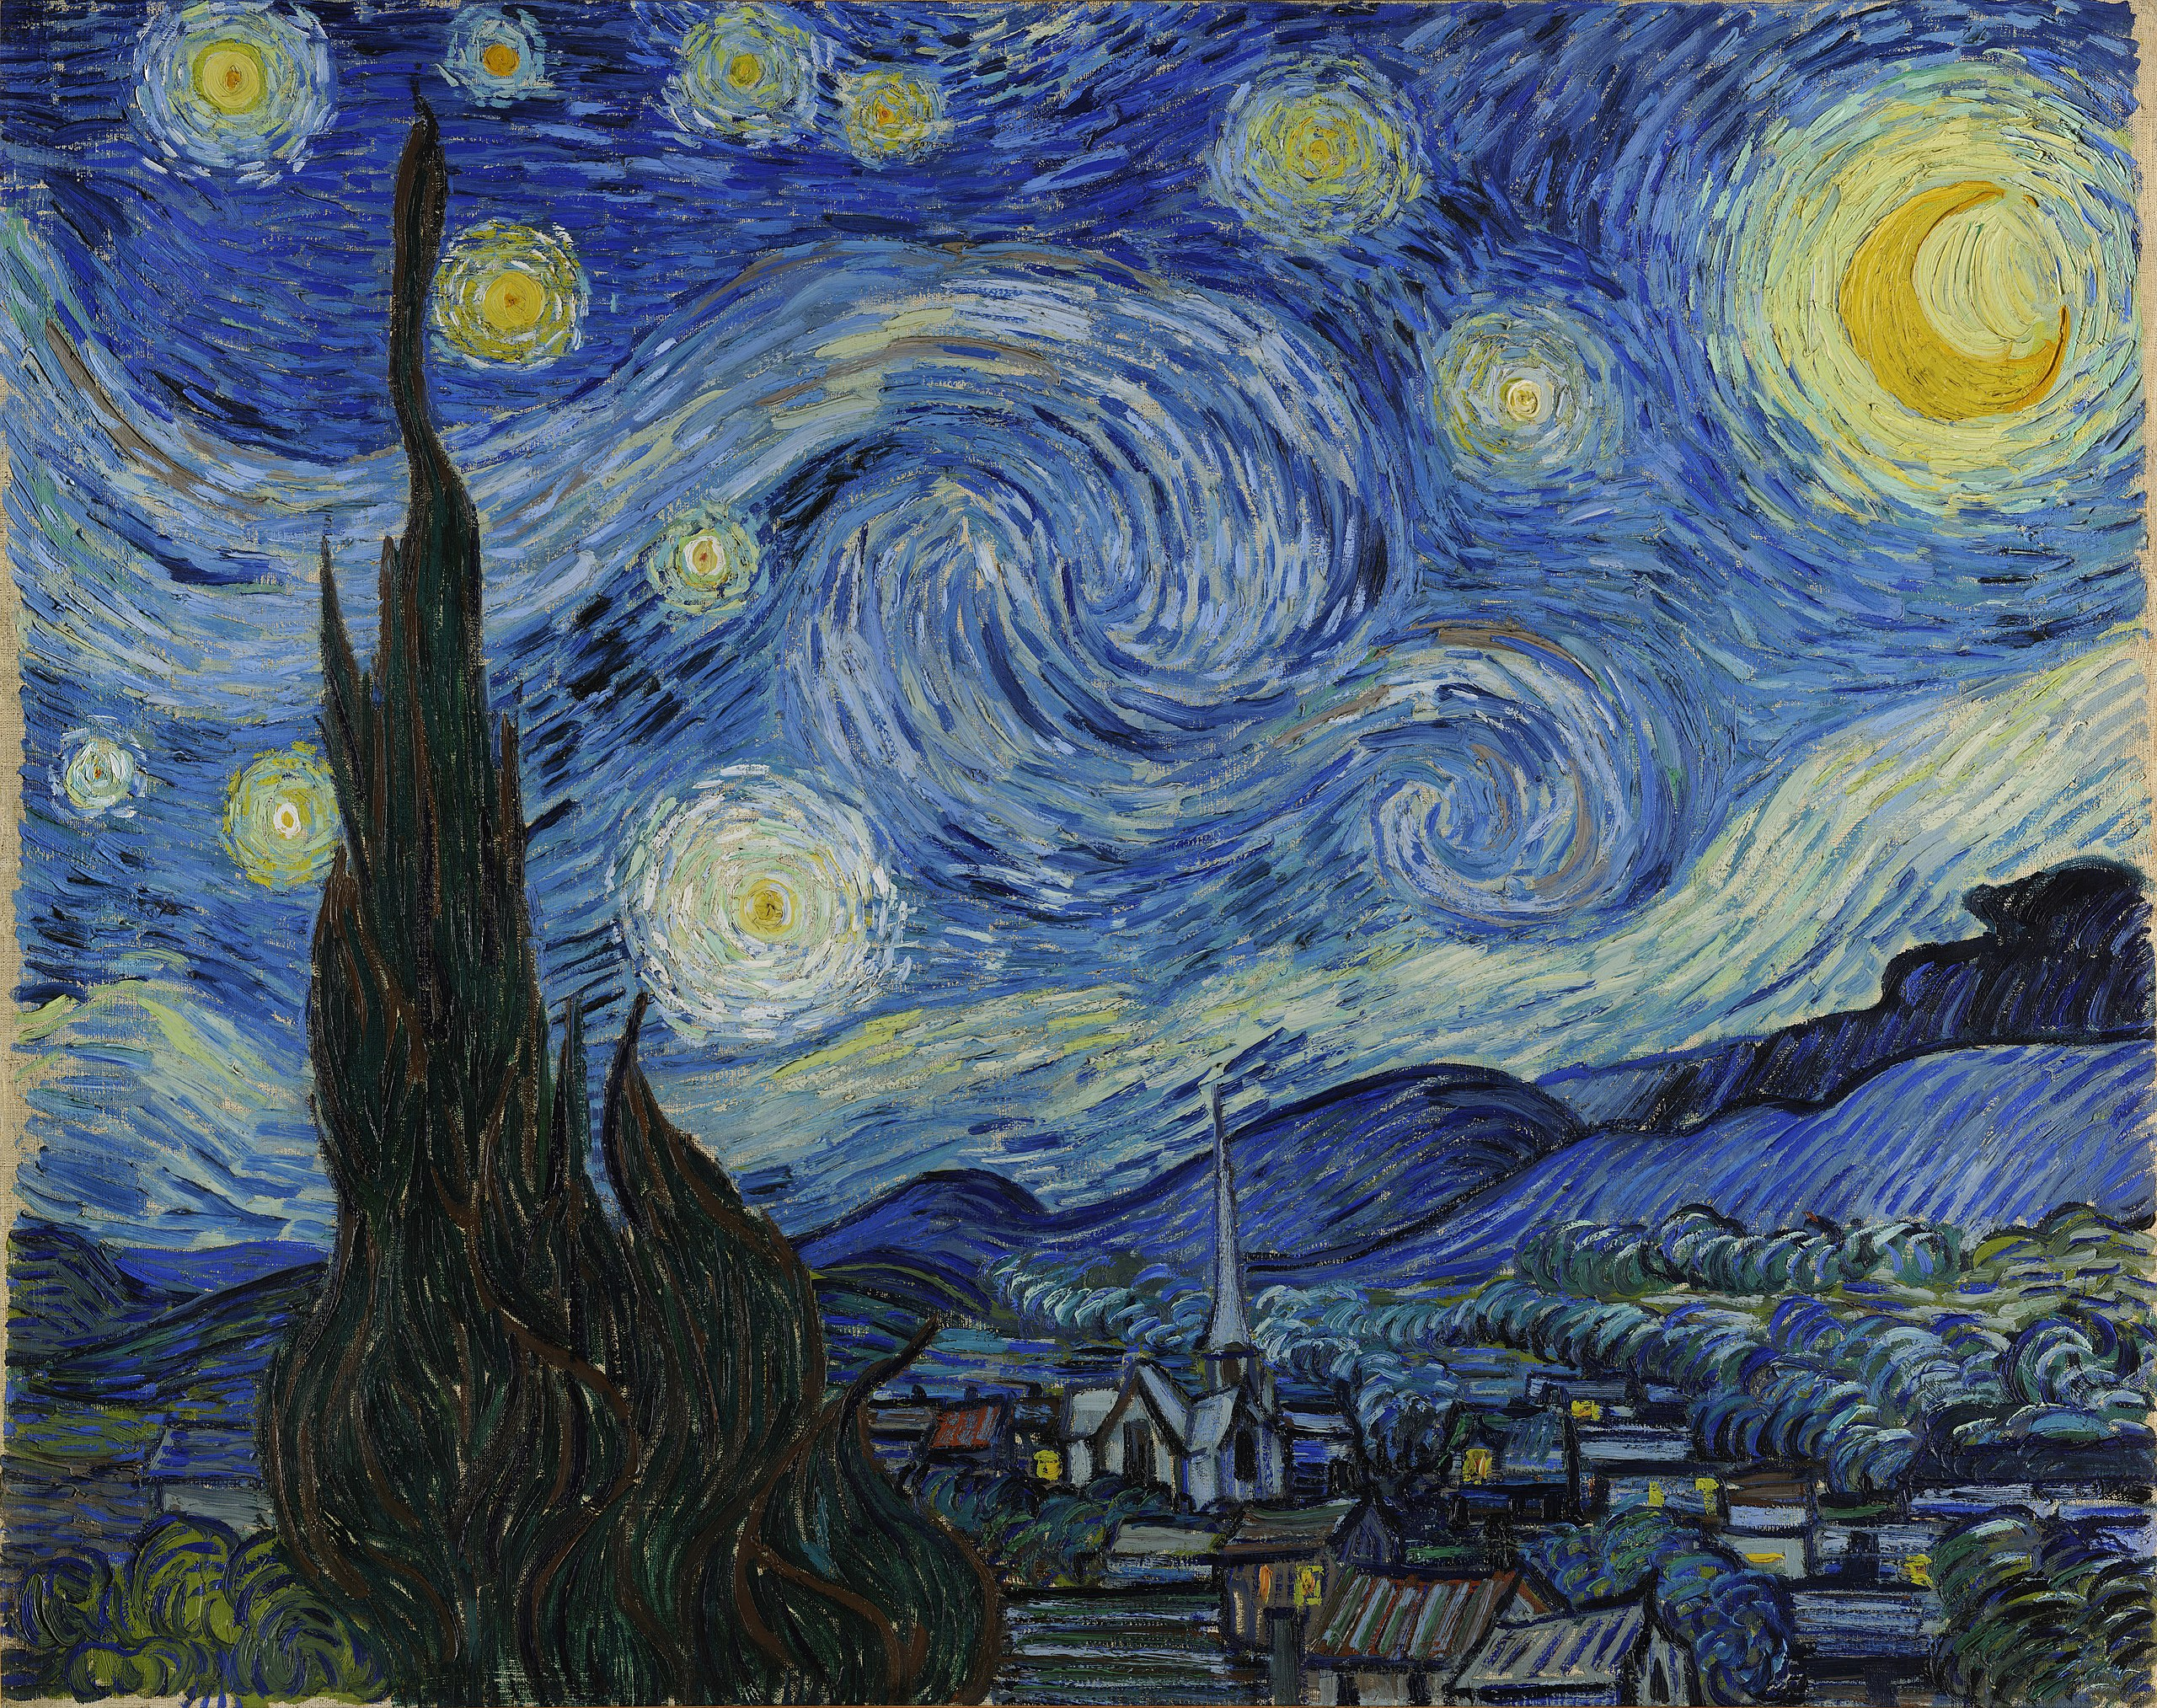
\includegraphics{figures/paintingexamples/starrynight}}
\caption{Like it or not, a continuous relation $[0,1] \rightarrow \blacksquare$: "The Starry Night", by Vincent van Gogh.}
\end{marginfigure}
\clearpage
\section{Populating space with shapes using sticky spiders}\label{sec:stickyspider}

%\begin{figure}\label{fig:spiderbicate}
%\scalebox{0.7}{\tikzfig{bestiary/spiderbicat}}
%\caption{The generators (in dashed boxes) and relations that make a spider. When the spider satisfies in addition the three inequalities b1-3, we call it a \textbf{relation-spider}.}
%\end{figure}

In this section, we seek to process-theoretically characterise disjoint collections of open sets of a space, so that we can play with doodles on the page as formal objects. It turns out that in \textbf{ContRel}, we can express them as idempotents that interact with spiders in a certain way.

\begin{example}[The copy-compare spiders of $\mathbf{Rel}$ are not always continuous]\label{ex:compnotspider}
The compare map for the Sierpi\'{n}ski space is not continuous, because the preimage of $\{0,1\}$ is $\{(0,0),(1,1)\}$, which is not open in the product space of $\mathcal{S}$ with itself.
\end{example}

\begin{rem}[copy-compare spiders of $\mathbf{Rel}$]
For a set $X$, the \emph{copy} map $X \rightarrow X \times X$ is defined:
\[\{(x,(x,x)) : x \in X \}\]
the \emph{compare} map $X \times X \rightarrow X$ is defined:
\[\{((x,x),x) : x \in X \}\]
These two maps are the (co)multiplications of special frobenius algebras. The (co)units are \emph{delete}:
\[\{(x,\star) : x \in X\}\]
and \emph{everything}:
\[\{(\star,x) : x \in X\}\]
\end{rem}

\newpage

\begin{myboxR}
\begin{proposition}\label{prop:copydiscrete}
The copy map is part of a special commutative frobenius algebra iff the topology is discrete.
\begin{proof}
Discrete topologies inherit the usual copy-compare spiders from \textbf{Rel}, so we have to show that when the copy map is part of a spider, the underlying wire must have a discrete topology. Suppose that some wire has a spider, and construct the following open set using an arbitrary point $p$:
\[\scalebox{0.5}{\tikzfig{structure/copyspiderproof/openpoint}}\]
It will suffice to show that this open set tests whether the input is the singleton $\{p\}$ -- when all singletons are open, the topology is discrete. As a lemma, we show that comparing distinct points $p \neq q$ yields the empty state.
\[\scalebox{0.5}{\tikzfig{structure/copyspiderproof/openpointproof}}\]
The (zero) implication follows since $p \neq q$ by assumption, so we know that deleting the comparison of $p$ and $q$ cannot be the unit scalar, and so must be the zero scalar, hence the comparison of $p$ and $q$ is the empty state. Now, the following case analysis shows that our open set only contains the point $p$.
\[\resizebox{0.75\textwidth}{!}{\tikzfig{structure/copyspiderproof/openpointcases}}\]
\end{proof}
\end{proposition}
\end{myboxR}

\begin{myboxB}
\begin{defn}[Sticky spiders]\label{defn:stickyspider}
A \textbf{sticky spider} (or just an $e$-spider, if we know that $e$ is a split idempotent), is a spider \emph{except} every identity wire on any side of an equation is replaced by the idempotent $e$.
\end{defn}

The desired graphical behaviour of a sticky spider is that one can still coalesce all connected spider-bodies together, but the 1-1 spider "sticks around" rather than disappearing as the identity. This is achieved by the following rules that cohere the idempotent $e$ with the (co)unit and (co)multiplications; they are the same as the usual rules for a special commutative frobenius algebra with two exceptions. First, where an identity wire appears in an equation, we replace it with an idempotent. Second, the monoid and comonoid components freely emit and absorb idempotents. By these rules, the usual proof [] for the normal form of spiders follows, except the idempotent becomes an explicit 1-1 spider, rather than the identity.
\[\resizebox{\textwidth}{!}{\tikzfig{structure/idemspider/stickyrelations}}\]
\end{myboxB}

\begin{myboxR}
\newthought{We can use split idempotents to transform copy-spiders from discrete topologies to sticky-spiders on other spaces.}
\begin{rem}[Split idempotents]
An \textbf{idempotent} in a category is a map $e: A \rightarrow A$ such that \[A \overset{e}{\rightarrow} A \overset{e}{\rightarrow} A = A \overset{e}{\rightarrow} A\]
A \textbf{split idempotent} is an idempotent $e: A \rightarrow A$ along with a \textbf{retract} $r: A \rightarrow B$ and a \textbf{section} $s: B \rightarrow A$ such that:
\[A \overset{e}{\rightarrow} A = A \overset{r}{\rightarrow} B \overset{s}{\rightarrow} A\]
\[B \overset{s}{\rightarrow} A \overset{r}{\rightarrow} B = B \overset{\mathop{id}}{\rightarrow} B\]
\end{rem}

We can graphically express the behaviour of a split idempotent $e$ as follows, where the semicircles for the section and retract $r,s$ form a visual pun. Recall that $X^\star$ denotes the discrete topology on the set $X$.

\[\scalebox{1}{\tikzfig{structure/idemspider/splitidem}}\]
\end{myboxR}

\begin{myboxB}
\begin{construction}[Sticky spiders from split idempotents]\label{cons:stickyfromsplit}
Given an idempotent $e: Y^\sigma \rightarrow Y^\sigma$ that splits through a discrete topology $X^\star$, we construct a new (co)multiplication as follows:
\[\scalebox{1}{\tikzfig{structure/idemspider/idemspiderv2}}\]
\end{construction}
\end{myboxB}

\begin{myboxR}
\begin{proposition}[Every idempotent that splits through a discrete topology gives a sticky spider]\label{prop:splitmeanssticky} The following is a sticky spider:
\[\scalebox{1}{\tikzfig{structure/idemspider/espiderstatement}}\]
\end{proposition}
We can check that Construction \ref{cons:stickyfromsplit} satisfies the frobenius rules as follows. We only present one equality; the rest follow the same idea.
\[\scalebox{1}{\tikzfig{structure/idemspider/espiderproofv2}}\]
\end{myboxR}
\begin{myboxR}
To verify the sticky spider rules, we first observe that since $X^\star \overset{s}{\rightarrow} Y^\sigma \overset{r}{\rightarrow} X^\star = X^\star \overset{\mathop{id}}{\rightarrow} X^\star$, $r$ must have all of $X^\star$ in its image, and $s$ must have all of $X^\star$ in its preimage, so we have the following:
\[\scalebox{1}{\tikzfig{structure/idemspider/splitonto}}\]
Now we show that e-unitality holds:
\[\scalebox{1}{\tikzfig{structure/idemspider/espiderproof2}}\]
The proofs of e-counitality, and e-speciality follow similarly.
\end{myboxR}

\begin{myboxB}
\newthought{We can prove a partial converse of Proposition \ref{prop:splitmeanssticky}:} we can identify two diagrammatic equations that tell us precisely when a sticky spider has an idempotent that splits though some discrete topology.
\begin{theorem}\label{thm:stickygraphical}
A sticky spider has an idempotent that splits through a discrete topology if and only if in addition to the sticky spider equalities, the following relations are also satisfied.
\[\scalebox{1}{\tikzfig{idemproof/unit-everything}} \quad\quad\quad\quad\quad\quad\quad\quad \scalebox{1}{\tikzfig{idemproof/comult-copy}}\]
\end{theorem}
The proof is involved, so here is a map of lemmas and propositions.
\[\resizebox{0.8\textwidth}{!}{\tikzfig{idemproof/claimmap2}}\]
\end{myboxB}

\begin{myboxR}
\begin{proposition}[comult/copy implies counit/delete]\label{prop:counitdelete}
\[\scalebox{1}{\tikzfig{idemproof/ecopy2delclaim}}\]
\begin{proof}
\[\scalebox{1}{\tikzfig{idemproof/ecopy2del}}\]
\end{proof}
\end{proposition}
\end{myboxR}

\begin{myboxB}
\begin{lemma}[All-or-Nothing]\label{lem:allornothing}
Consider the set $e(\{x\})$ obtained by applying the idempotent $e$ to a singleton $\{x\}$, and take an arbitrary element $y \in e(x)$ of this set. Then $e(\{y\}) = \varnothing$ or $e(\{x\}) = e(\{y\})$. Diagrammatically: \[\scalebox{0.75}{\tikzfig{idemproof/allornothingclaim}}\]
\end{lemma}
\[\scalebox{0.75}{\tikzfig{idemproof/allornothing2a}}\]
\end{myboxB}
\begin{myboxB}
\[\scalebox{0.75}{\tikzfig{idemproof/allornothing2b}}\]
\end{myboxB}

\begin{myboxR}
\begin{proposition}[$e$ of any point is $e$-copiable]\label{prop:epointcopy}
\[\scalebox{0.75}{\tikzfig{idemproof/pointidemcopiable}}\]
\begin{proof}
\[\scalebox{0.75}{\tikzfig{idemproof/pointidemcopiableproof}}\]
\end{proof}
\end{proposition}
\end{myboxR}

\begin{myboxB}
\begin{proposition}[The unit is the union of all $e$-copiables]\label{prop:copiablebasis}
\[\scalebox{0.8}{\tikzfig{idemproof/copiablebasisclaim}}\]
\begin{proof}
\[\scalebox{0.8}{\tikzfig{idemproof/copiablebasis}}\]
\end{proof}
\end{proposition}
\end{myboxB}

\begin{myboxR}
\begin{proposition}[$e$-copiable decomposition of $e$]\label{prop:decompidem}
\[\scalebox{1}{\tikzfig{idemproof/decompidemclaim}}\]
\begin{proof}
\[\scalebox{1}{\tikzfig{idemproof/decompidem}}\]
\end{proof}
\end{proposition}
\end{myboxR}

\begin{myboxB}
\begin{proposition}[$e$-copiable decomposition of counit]\label{prop:decompcounit}
\[\scalebox{1}{\tikzfig{idemproof/decompcounitclaim}}\]
\begin{proof}
\[\scalebox{1}{\tikzfig{idemproof/decompcounit}}\]
\end{proof}
\end{proposition}
\end{myboxB}

\begin{myboxR}
\newthought{The $e$-copiable states really do behave like an orthonormal basis, as the following Lemmas show.}
\begin{lemma}[$e$-copiables are orthogonal under multiplication]\label{lem:match}
\[\scalebox{0.75}{\tikzfig{idemproof/matchclaim}}\]
\begin{proof}
\[\scalebox{0.75}{\tikzfig{idemproof/match}}\]
\end{proof}
\end{lemma}
\end{myboxR}

\begin{myboxB}
\begin{convention}[Shorthand for the open set associated with an $e$-copiable]
We introduce the following diagrammatic shorthand.
\[\scalebox{1}{\tikzfig{idemproof/openshorthand}}\]
Including the coloured dot is justified, because these open sets are co-copiable with respect to the multiplication of the sticky spider.
\[\scalebox{1}{\tikzfig{idemproof/shorthandjustification}}\]
\end{convention}
\end{myboxB}

\begin{myboxR}
\begin{lemma}[Co-match]\label{lem:comatch}
\[\scalebox{1}{\tikzfig{idemproof/comatchclaim}}\]
\begin{proof}
\[\scalebox{0.9}{\tikzfig{idemproof/comatch}}\]
The claim then follows by applying Lemma \ref{lem:match} to the final diagram.
\end{proof}
\end{lemma}
\end{myboxR}

\begin{myboxB}
\begin{lemma}[e-copiables are e-fixpoints]\label{lem:ecopyfixpoint}
\[\scalebox{1}{\tikzfig{idemproof/dotcopyableclaim}}\]
\begin{proof}
\[\scalebox{1}{\tikzfig{idemproof/dotcopyable}}\]
Observe that the final equation of the proof also holds when the initial e-copiable is the empty set.
\end{proof}
\end{lemma}
\end{myboxB}

\begin{myboxR}
\begin{lemma}[$e$-copiables are normal]\label{lem:ecopynormal}
\[\scalebox{1}{\tikzfig{idemproof/copynormalclaim}}\]
\begin{proof}
\[\scalebox{1}{\tikzfig{idemproof/copynormal}}\]
\end{proof}
\end{lemma}
\end{myboxR}

\begin{myboxB}
\begin{proposition}[$e$-copiable decomposition of multiplication]\label{prop:decompmult}
\[\scalebox{1}{\tikzfig{idemproof/decompmultclaim}}\]
\begin{proof}
\[\scalebox{1}{\tikzfig{idemproof/decompmult}}\]
\end{proof}
\end{proposition}
\end{myboxB}

\begin{myboxR}
\begin{proposition}[$e$-copiable decomposition of comultiplication]\label{prop:decompcomult}
\[\scalebox{1}{\tikzfig{idemproof/decompcomultclaim}}\]
\begin{proof}
\[\scalebox{1}{\tikzfig{idemproof/decompcomult}}\]
\end{proof}
\end{proposition}
\end{myboxR}

\begin{myboxB}
\newthought{Now we can prove Theorem \ref{thm:stickygraphical}.}
First a reminder of the claim; we want to show that when given a sticky spider, the following relations hold if and only if the idempotent splits through a discrete topology.
\[\scalebox{0.8}{\tikzfig{idemproof/unit-everything}} \quad\quad\quad\quad\quad\quad\quad\quad \scalebox{0.8}{\tikzfig{idemproof/comult-copy}}\]
The crucial observation is that the $e$-copiable decomposition of the idempotent given by Proposition \ref{prop:decompidem} is equivalent to a split idempotent though the set of $e$-copiables equipped with discrete topology.
\[\scalebox{0.8}{\tikzfig{idemproof/finalproof}}\]
By copiable basis Proposition \ref{prop:copiablebasis} and the decompositions Propositions \ref{prop:decompcounit}, \ref{prop:decompmult}, \ref{prop:decompcomult}, we obtain the only-if direction.
\[\scalebox{0.8}{\tikzfig{idemproof/finalproof2}}\]
\end{myboxB}
\begin{myboxB}
The if direction is an easy check. For the unit/everything relation, we have:
\[\scalebox{0.8}{\tikzfig{idemproof/finalproof3}}\]
For the counit/delete relation, we observe that for any split idempotent, the retract must be a partial function. To see this, suppose the split idempotent $e = r;s$ is on $(X,\tau)$ and the discrete topology is $Y^\star$. Seeking contradiction, if the retract is not a partial function, then there is some point $x \in X$ such that $x \in e(x)$, and the image $I := r(x) \subseteq Y$ contains more than one point, which we denote and discriminate $a,b \in r(x) \subseteq Y$ and $a \neq b$. Because the composite $s;r = 1_Y$ of the section and retract must recover the identity on $Y^\star$, the section $s$ must be total -- i.e. the image $s(X) = Y$. So $x \in s(a) \cap s(b)$. Now we have that $(a,x),(b,x) \in s$, and $(x,a),(x,b) \in r$, therefore $(a,b),(b,a) \in s;r$, which by $a \neq b$ contradicts that $s;r$ is the identity relation $1_Y$.
\[\scalebox{0.8}{\tikzfig{idemproof/finalproof4}}\]
\end{myboxB}

\begin{myboxR}
\begin{defn}[Labels, shapes, cores, halos]
Recall by Proposition \ref{prop:decompidem} that we can express the idempotent as a union of continuous relations formed of a state and test, for some indexing set of \emph{labels} $\mathcal{L}$.
\[\tikzfig{topology/shape1}\]
A \emph{shape} is a component of this union corresponding to some arbitary $l \in L$. So we refer to a sticky spider as a labelled collection of shapes. The state of a shape is the \emph{halo} of the shape. The halos are precisely the copiables of the sticky spider. The test of a shape is the \emph{core}. The cores are precisely the cocopiables of the sticky spider.
\[\tikzfig{topology/shape2}\]
\end{defn}
\end{myboxR}

\begin{myboxB}
\begin{proposition}[Core exclusion: Distinct cores cannot overlap]\label{prop:core-core-exclusion}
\begin{proof}
A direct consequence of Lemma \ref{lem:comatch}.
\end{proof}
\end{proposition}
\end{myboxB}

\begin{myboxR}
\begin{proposition}[Core-halo exclusion: Each core only overlaps with its corresponding halo]\label{prop:core-halo-exclusion}
\begin{proof}
Seeking contradiction, if a core overlapped with multiple halos, Lemma \ref{lem:ecopyfixpoint} would be violated.
\end{proof}
\end{proposition}
\end{myboxR}

\begin{myboxB}
\begin{proposition}[Halo non-exclusion: halos may overlap]
\begin{proof}
By example:
\[\tikzfig{topology/halooverlap}\]
The two shapes are colour coded cyan and magenta. The halos are two triangles which overlap at a yellow region, and partially overlap with their blobby cores. The cores are outlined in dotted blue and orange respectively. Observe that cores and halos do not have to be simply connected; in this example the core of the magenta shape has two connected components. Viewing these sticky spiders as a process, any shape that overlaps with the magenta core will be deleted and replaced by the magenta triangle, and similarly with the cyan cores and triangle. Any shape that overlaps with both the magenta and cyan cores will be deleted and replaced by the union of the triangles. Any shape that overlaps with neither core will be deleted and not replaced.
\end{proof}
\end{proposition}
\end{myboxB}

\begin{myboxR}
\begin{corollary}[Only opens please]
A sticky spider corresponds to a set-indexed disjoint collection of open sets when, in addition to the equations of Theorem \ref{thm:stickygraphical}, it satisfies one more, depicted below on the left.
\[\scalebox{1}{\tikzfig{idemproof/opensonly}}\]
Observe that the right hand equation above is precisely what we want expressed in diagrams: that every halo matches its core. For the forward direction, we have:
\[\scalebox{1}{\tikzfig{idemproof/opensonly3}}\]
\end{corollary}
\end{myboxR}

\begin{myboxR}
For the backward direction, we rely on the fact that cores are non-empty (or else we would fail to satisfy the identity equation of the split idempotent) to eliminate the floating scalars.
\[\scalebox{1}{\tikzfig{idemproof/opensonly2}}\]
By Proposition \ref{prop:core-core-exclusion}, we have disjointness.\\

So, without loss of generality, we may treat any collection of disjoint open shapes on a page as a sticky spider.
\end{myboxR}

\clearpage
\clearpage
\section{Basic topological concepts in flatland via \textbf{ContRel}}\label{sec:concepts}

The goal now is to demonstrate the use of the sticky spiders we have obtained in the previous section as formal semantics for the kinds of schematic doodles or cartoons we would like to draw. Throughout we consider sticky spiders on $\mathbb{R}^2$. In service of defining \emph{configuration spaces} of shapes up to rigid displacement, we diagrammatically characterise the topological subgroup of isometries of $\mathbb{R}^2$ by building up in the diagrammatic presentations of the unit interval, metrics, and topological groups. To further isolate rigid displacements that arise from continuous sliding motion of shapes in the plane (thus excluding displacements that result in mirror-images), we diagrammatically characterise an analogue of homotopy in the relational setting. Finally, in we build up a stock of topological concepts and study by examples how implementing these concepts within text circuits explains some idiosyncrasies of the theory: namely why noun wires are labelled by their noun, why adjective gates ought to commute, and why verb gates do not.

\newthought{Itinerary of upcoming examples and definitions:} I would like to say it's obvious how to make shapes move and tell when they are touching and so on, but you may not believe me. So, I am going to recover a fair chunk of elementary topology diagrammatically in \textbf{ContRel}.

\newthought{Shapes and places} We can already do interesting things with just sticky spiders. In Example \ref{ex:chessboard}, we show how we can use sticky spiders to tell how pieces are on a chessboard. How is it that pieces on a chessboard in \emph{continuous} space are translated into \emph{discrete} data, such as \texttt{pawn on e4}?

\newthought{The reals}
To begin modelling more complex concepts, we first need to extend our topological tools. The first stop is the reals. There are many spaces homeomorphic to the real line. How do we know when we have one of them? The following theorem provides an answer:
\begin{theorem}[Friedman]\label{thm:Friedman}
Let $\big((X,\tau), < \big)$ be a topological space with a total order. If there exists a continuous map $f: X \times X \rightarrow X$ such that $\forall a,b_{\in X} : a < f(a,b) < b$, then $X$ is homeomorphic to $\mathbb{R}$. \citep{friedman_fom_2005}
\end{theorem}
We diagrammatically characterise total orders in Definition \ref{defn:lessthan}. Here Trichotomy requires us to appeal to the rig structure so that we can access unions of processes explicitly. Going forward we will also introduce quantifiers into process-theoretic equations, essentially treating process-equations as we would any other symbolic algebraic specification. Then we express Friedman's theorem using diagrammatic equations in Definition \ref{defn:friedfunct}.

\newthought{The unit interval}
If we have the unit interval, we can begin to define what it would mean for spaces to be connected (by drawing lines between points in those spaces), and we can also move towards defining motion as movement along a line. To obtain the unit interval (up to homeomorphism) we need to add endpoints to $\mathbb{R}$. We can introduce endpoints for open intervals directly by asking for the space $X$ to have points that are less than or greater than all other points. Another method, which we will use here for primarily aesthetic reasons, is to use endocombinators to define suprema. For a motivating example of the ubiquity of endocombinators, consider the case when we have a locally indiscrete topology:
\begin{defn}[Locally indiscrete topology]
$(X,\tau)$ is \emph{locally indiscrete} when every open set is also closed.
\end{defn}
If we know that a topology is locally indiscrete and we are given an open $U$, we would like to notate the complement $X/U$ -- which we know to be open -- as any of the following, which only differ up to notation.
\[\resizebox{0.5\textwidth}{!}{\tikzfig{topology/negbubble}}\]
Unfortunately, the complementation operation $X/-$ is not in general a continuous relation, hence in the lattermost expression above we resort to using bubbles -- endocombinators -- as syntactic sugar. Endocombinators are like functional expressions applied to diagrams: the semantics and notation for which we borrow and modify from \citep{haydon_compositional_2020}.
\begin{defn}[Partial endocombinator]
In a category $\mathcal{C}$, a \emph{partial endocombinator} on a homset $\mathcal(C)(A,B)$ is a function $\mathcal(C)(A,B) \rightarrow \mathcal(C)(A,B)$
\end{defn}

\newthought{Simply connected shapes and spaces}

Once we have a unit interval, we can define the usual topological notion of a simply connected space (Definition \ref{def:simpconn}): one where any two points can be connected by a continuous line without leaving the space.

\newthought{Displacing shapes}

Static shapes in space are nice, but moving them around would be nicer. So we have to define a stock of concepts to express rigid motion. Rigidity however is a difficult concept to express in topological spaces up to homeomorphism -- everyone is well aware of the popular gloss of topology in terms of coffee cups being homeomorphic to donuts. To obtain rigid transformations as we have in Euclidean space, we need to define metrics (Definition \ref{def:metric}), and in order to do that, we need addition (Definition \ref{def:addition}).

\newthought{Rigid displacements}

Then we return to sticky spiders and we restrict our consideration to those on the open unit square, so that we can speak of shapes on a canvas. We want to rigidly displace the shapes of a sticky spider, which is obtained via the notions of isometries (Definition \ref{def:isometry}) and topological groups (Definition \ref{def:topgrp}).

\begin{remark}
When we draw on a finite canvas representing all of euclidean space, properly there should be a fishbowl effect that relatively magnifies shapes close to the origin and shrinks those at the periphery, but that is only an artefact of representing all of euclidean space on a finite canvas. Since all the usual metrics are still really there, going forward we will ignore this fishbowl effect and just doodle shapes as we see fit.
\[\tikzfig{topology/fisheye}\]
\end{remark}

\newthought{Motion of rigid bodies}

To obtain continuous transformations in the plane from the configuration of shapes in one spider to end at the configuration of shapes in another, we define a conservative generalisation of \emph{homotopy}: the continuous deformation of one map to another (Definition \ref{defn:homotopy}). A side benefit we obtain is that when we have homotopies, we can also define contractible shapes, which are connected and have no holes. Then we define configuration spaces of shapes on the plane so we can talk about all permissible positions shapes may be in, and at last we can define motions of rigid bodies.

\newthought{Modelling linguistic topological concepts}

By "linguistic", I mean to refer to the kinds of concepts we use in everyday language, and by "topological" I \emph{don't} mean spatial relationships that are invariant under homeomorphism (as recall, we deal primarily with rigid and finitely deformable objects in our day-to-day). I mean to refer to non-metric and non-directional spatial relationships such as parthood, touching, within/surrounds, containment/entrapment, interlocking, and mutually constrained motions. These are concepts that even very young children have an intuitive grasp of \citep{jean_childs_1967}, but their formal definitions are difficult to pin down. One such relation modelled here -- touching -- is in fact a \emph{semantic prime} \citep{wierzbicka_semantics_1996}: a word that is present in essentially all natural languages that is conceptually primitive, in the sense that it resists definition in simpler terms. It is among the ranks of concepts like \emph{wanting} or \emph{living}, words that are understood by the experience of being human, rather than by school. As such, I make no claim that these definitions are canonical, just that they are good enough to reason with. Then I will introduce some dynamic relationships such as collision, along with some remarks on how vignettes may be composed out of homotopies and a general recipe for obtaining homotopies that -- via deformation -- relate any pair of sticky spiders with the same number of shapes. This analysis extends to talk of rigid and deforming bodies and the manner, order, and coordination of their movement and interaction in any space.

\newthought{Thus, I consider any linguistic semantics that can be grounded in mechanical or tabletop models, to be formal.} By Example \ref{ex:chessboard}, we have enough technology to speak of locations in space, so we have access to "tabletop semantics": anything that in principle can be represented by counters and meeples in a boardgame, with for instance reserved spaces on the board for health and hunger and whatever else is necessary. The analysis of rigid bodies is hopefully sufficient to demonstrate that, in principle, one may linguistically characterise mechanical models, and there are a lot of mechanical models, including: mechanically realised clocks [duh.], analogues of electric circuits \citep{noauthor_spintronics_nodate}, computers \citep{richard_ridel_mechanical_2015}, and human-like automata \citep{wikipedia_authors_jaquet-droz_2022}. Of course in reality mechanical motions are reversible among rigid objects, and directional behaviour is provided by a source of energy, such as gravitational potential, or wound springs. But we may in principle replace these sources of energy by a belt that we choose to spin in one direction -- our own arrow of time.

\newthought{\textbf{Objection:} That is way outside the scope of formal semantics.} Insofar as semantics is sensemaking, we certainly are capable of making sense of things in terms of mechanical models and games by means of metaphor, the mathematical treatment of which is concern of Section \ref{sec:metaphor}. Part of the reason I went through the trouble of deriving linguistic topological relations from nothing is so that I can claim that by any sensible definition, I am doing formal semantics for natural language. Whether or not I'm exceeding the scope of what a linguist might consider formal semantics is ultimately irrelevant, as I am not concerned with the modal human mechanism, only with process-theoretic characterisations of things, because they tend to be worthwhile practically. There is maybe also a prejudice that formal semantics must necessarily resolve in some symbolic logic, to which I might charitably respond that I'm working with an algebraic system, just not a one-dimensional one. Less charitably, I don't care what you think linguistics ought to be.

\newpage

\begin{myboxB}
\begin{example}[Where is a piece on a chessboard?]\label{ex:chessboard}
How is it that we quotient away the continuous structure of positions on a chessboard to locate pieces among a discrete set of squares? Evidently shifting a piece a little off the centre of a square doesn't change the state of the game, and this resistance to small perturbations suggests that a topological model is appropriate. We construct two spiders, one for pieces, and one for places on the chessboard. For the spider that represents the position of pieces, we open balls of some radius $r$, and we consider the places spider to consist of square halos (which tile the chessboard), containing a core inset by the same radius $r$; in this way, any piece can only overlap at most one square. As a technical aside, to keep the core of the tiles open, we can choose an arbitrarily sharp curvature $\epsilon$ at the corners.
\[\scalebox{0.70}{\tikzfig{topology/chessboard}}\]
Now we observe that the calculation of positions corresponds to composing sticky spiders. We take the initial state to be the sticky spider that assigns a ball of radius $r$ on the board for each piece. We can then obtain the set of positions of each piece by composing with the places spider. The composite (pieces;places)
will send the king to a2, the bishop to b4, and the knight to d1, i.e. $\bra{K} \mapsto \bra{a2}$, $\bra{B} \mapsto \bra{b4}$ and $\bra{N} \mapsto \bra{d1}$. In other words, we have obtained a process that models how we pass from continuous states-of-affairs on a physical chessboard to an abstract and discrete game-state.
\[\resizebox{0.70\textwidth}{!}{\tikzfig{topology/chessboard2a}}\]
\end{example}
\end{myboxB}

\begin{myboxR}
\begin{defn}[Less than]\label{defn:lessthan}
We define a total ordering relation $<$ as an open set on $X \times X$ that obeys the usual axiomatic rules:
\[\resizebox{\textwidth}{!}{\tikzfig{topology/lessthan}}\]
\[\tikzfig{topology/lessthantotal}\]
\end{defn}
\end{myboxR}

\begin{myboxB}
\begin{defn}[Friedman's function]\label{defn:friedfunct}
Just as a wire in \textbf{ContRel} has the discrete topology if it possesses spider structure (Proposition \ref{prop:copydiscrete}), a wire is homeomorphic to the real line by Theorem \ref{thm:Friedman} if it possesses an open that behaves as Definition \ref{defn:lessthan}, and a map that satisfies:
\[\tikzfig{topology/betweenfunct}\]
\end{defn}
\end{myboxB}

\begin{myboxR}
\begin{defn}[Upper and lower bounds via endocombinators]\label{defn:bounds}
Upper bounds are endocombinators that send states to points. This is an equational condition quantified over all states.
\[\tikzfig{topology/upperbound}\]
\end{defn}
We can add in further equations governing the upper bound endocombinator to turn it into a supremum, where the lower endpoint is obtained as the supremum of the empty set, and the upper endpoint is the supremum of the whole set.
\begin{defn}[Suprema]\label{defn:sup}
\[\tikzfig{topology/sup}\]
\end{defn}
\begin{defn}[Endpoints]\label{defn:endpoints}
Now we can define endpoints purely graphically. The lower endpoint is the supremum of the empty state, and the upper the supremum of everything.
\[\tikzfig{topology/endpoints}\]
\end{defn}
Going forward, we will denote the unit interval using a thick dotted wire.

\end{myboxR}

\begin{myboxB}
\begin{defn}[Simple connectivity]\label{def:simpconn}
Recall that we notate points and functions with the same small black dot for copying and deleting, as points are precisely the states that are copy-delete cohomomorphisms. In prose, simple connectivity states that for any pair of points that are within the open $V$, there exists some continuous function from the unit interval into the space that starts at one of the points and ends at the other. The left pair of conditions state that the points $\textcolor{blue}{x}$ and $\textcolor{red}{y}$ are within $V$. The right triple of conditions require the the image of the homotopy $\textcolor{orange}{f}$ is contained in $V$, and that its endpoints are $\textcolor{blue}{x}$ and $\textcolor{red}{y}$.
\[\tikzfig{topology/simplyconnected}\]
Simple connectivity is a useful enough concept that we will notate simply connected open sets as follows, where the hole is a reminder that simply connected spaces might still have holes in them.
\[\tikzfig{topology/simpconnotation}\]
\end{defn}
\end{myboxB}

\begin{myboxR}
\begin{defn}[Addition]\label{def:addition}
In order to define metrics, we must have additive structure, which we encode as an additive monoid that is a function. All we need to know is that the lower endpoint of the unit interval stands in for "zero distance" -- as the unit of the monoid -- and that adding positive distances together will deterministically give you a larger positive distance.
\[\resizebox{\textwidth}{!}{\tikzfig{topology/addition}}\]
\end{defn}
\end{myboxR}

\begin{myboxB}
\begin{defn}[Metric]\label{def:metric}
A metric on a space is a continuous map $X \rightarrow \mathbb{R}^+$ to the positive reals that satisfies these axioms. We depict metrics as trapezoids.
\end{defn}
\[\resizebox{\textwidth}{!}{\tikzfig{topology/metric}}\]
\end{myboxB}

\begin{myboxR}
\begin{defn}[Open balls]\label{def:openball}
Once we have metrics, we can define the usual topological notion of open balls. With respect to a metric, an $\varepsilon$-open ball at $\textcolor{blue}{x}$ is the open set (effect) of all points that are $\varepsilon$-close to $\textcolor{blue}{x}$ by the chosen metric.
\[\tikzfig{topology/openball2}\]
Open balls will come in handy later, and a side-effect which we note but do not explore is that open balls form a basis for any metric space, so in the future whenever we construct spaces that come with natural metrics, we can speak of their topology without any further work.
\end{defn}
\end{myboxR}

\begin{myboxB}
With metrics in hand, we can proceed to define isometries as topological groups that keep distances invariant.
\begin{defn}[Topological groups]\label{def:topgrp} 
It is no trouble to depict collections of invertible transformations of spaces $X \rightarrow X$.
\[\tikzfig{topology/topologicalgroup}\]
A consequence of invertibility and the requirement that the identity transform is a group element forces all transformations in a topological group to be functions.
\end{defn}
\begin{defn}[Isometry]\label{def:isometry}
An isometry is a distance preserving transformation: applying the metric pointwise before and after a topological group action gives the same value.
\[\tikzfig{topology/isometry}\]
\end{defn}
\end{myboxB}

\begin{myboxB}
\begin{defn}[Planar isometries]\label{defn:planarisometry}
We know the planar isometries of Euclidean space can be expressed as a translation, rotation, and an addition bit of data to indicate the chirality of the shape -- as mirror reflections are also an isometry. In flatland, we do not expect shapes to suddenly flip over. We would like to express just those rigid transformations that leave the chirality of the shape intact, because really we want to only be able to slide the shapes around the canvas, not leave the canvas to flip over.
\[\tikzfig{topology/planeisometries}\]
With this in mind, we have the following condition relating different spiders on the unit square, telling us when one is the same as the other up to rigidly displacing shapes.
\[\tikzfig{topology/displacerigid}\]
\end{defn}
\end{myboxB}

\begin{myboxR}
\begin{remark}\label{remark:homotopywrinkle}
Usually, when we are restricted to speaking of topological spaces and continuous functions, a homotopy is defined:
\end{remark}

\begin{defn}[Homotopy in \textbf{Top}]
where $f$ and $g$ are continuous maps $A \rightarrow B$, a \emph{homotopy} $\eta : f \Rightarrow g$ is a continuous function $\eta : [0,1] \times A \rightarrow B$ such that $\eta(0,-) = f(-)$ and $\eta(1,-) = g(1,-)$.
\end{defn}

In other words, a homotopy is like a short film where at the beginning there is an $f$, which continuously deforms to end the film being a $g$. Directly replacing "function" with "relation" in the above definition does not quite do what we want, because we would be able to define the following "homotopy" between open sets.

\[\tikzfig{topology/homotopyctrex1}\]

What is happening in the above film is that we have our starting open set, which stays constant for a while. Then suddenly the ending open set appears, the starting open disappears, and we are left with our ending; while \emph{technically} there was no discontinuous jump, this isn't the notion of sliding we want. The exemplified issue is that we can patch together (by union of continuous relations) vignettes of continuous relations that are not individually total on $[0,1]$.
\end{myboxR}

\begin{myboxB}
\begin{defn}[Relational Homotopy]\label{defn:homotopy}
We can patch the issue in Remark \ref{remark:homotopywrinkle} by asking for homotopies in \textbf{ContRel} to satisfy the additional condition that they are expressible as a union of continuous partial maps that are total on the unit interval.
\[\tikzfig{topology/homotopy}\]
\end{defn}
\end{myboxB}

\begin{myboxR}
\begin{remark}
Observe that the second condition asking for decomposition in terms of partial comes for free by Proposition \ref{prop:hombasis}; the constraint of the definition is provided by the first condition, which is a stronger condition than just asking that the original continuous relation be total on $I$:
\[\tikzfig{topology/homotopyctrex1}\]
Definition \ref{defn:homotopy} is "natural" in light of Proposition \ref{prop:hombasis}, that the partial continuous functions $A \rightarrow B$ form a basis for $\mathbf{ContRel}(A,B)$: we are just asking that homotopies between partial continuous functions -- which can be viewed as regular homotopies with domain restricted to the subspace topology induced by an open set -- form a basis for homotopies between continuous relations.
\[\tikzfig{topology/homotopyctrex}\]
\end{remark}
\end{myboxR}

\begin{myboxB}
\begin{defn}[Contractibility]\label{defn:contractible}
With homotopies in hand, we can define a stronger notion of connected shapes with no holes, which are usually called \emph{contractible}. The reason for the terminology reflects the method by which we can guarantee a shape in flatland has no holes: when any loop in the shape is \emph{contractible} to a point.
\[\resizebox{\textwidth}{!}{\tikzfig{topology/contractible}}\]
Contractible open sets are worth their own notation too; a solid black effect, this time with no hole.
\[\tikzfig{topology/contractnotation}\]
\end{defn}
\end{myboxB}

\begin{myboxR}
\begin{defn}[Touching]\label{defn:touching}
Let's distinguish touching from overlap. Two shapes are "touching" intuitively when they are as close as they can be to each other, somewhere; any closer and they would overlap. Let's assume that we can restrict our attention to the parts of the shape that are touching, and that we can fill in the holes of these parts. At the point of touching, there is an infinitesimal gap -- just as when we touch things in meatspace, there is a very small gap between us and the object due to the repulsive electromagnetic force between atoms. To deal with infinitesimals we borrow the $\epsilon-\delta$ trick from mathematical analysis; for any arbitrarily small $\delta$, we can pick an even smaller ball of radius $\epsilon$ such that if we stick the ball in the gap, the ball forms a bridge that overlaps the two filled-in shapes, which allows us to draw a continuous line between them. Diagrammatically, this is: 
\[\resizebox{\textwidth}{!}{\tikzfig{topology/touching}}\]
\end{defn}
\end{myboxR}

\begin{myboxB}
\begin{defn}[Within and surrounds]\label{defn:within}
If $U$ surrounds $V$, or equivalently, if $V$ is within $U$, then we are saying that leaving $V$ in almost any direction, we will see some of $U$ before we go off to infinity. We can once again use open balls for this purpose, which correspond to possible places you can get to from a starting point $\mathbf{x}$ within a distance $\epsilon$. In prose, we are asking that any open ball that contains all of $U$ must also contain all of $V$.
\[\tikzfig{topology/within}\]
\end{defn}
\end{myboxB}

\begin{myboxR}
\begin{defn}[Containment and enclosure]\label{defn:containment}
There is a strong version of within-ness, which we will call enclosure. As in when we are in elevators and the door is shut, nothing gets in or out of the container. Intuitively, there is a hole in the container surrounded on all sides, and the contained shape lives within the hole. To give a real-world example, honey lives within a honeycomb cell in a beehive, but whether the honey is enclosed in the cell depends on whether it is sealed off from air with beeswax. So in prose we are asking that any way we fill in the holes of the container with a blob, that blob must cover the contained shape. Diagrammatically, this amounts to levelling up from open balls in our previous definition to contractible sets:
\[\tikzfig{topology/enclose}\]
\end{defn}
\end{myboxR}


\begin{myboxB}
\begin{defn}[Trapping]\label{defn:trapped}
There is an intermediate notion between within-ness and enclosure; for instance, standing in the stonehenge you are surrounded by the pillars, but you can always walk away, whereas if the pillars are very close, such as the bars of a jail cell, a human would not be able to leave the trap while still being able to see the outside. The difficulty here is that relative sizes come into play: small animals would still consider it a case of mere within-ness, because they can still walk away between the bars. So we would like to say that no matter how the pair of objects move rigidly, being trapped means that the trapped $V$ stays within $U$. In other words, that in configuration space, if we forget about all other shapes, we can partition our space of configurations by two concepts, whether $V$ is within $U$ or not, and moreover that these two components is disjoint -- i.e. not simply connected -- so there is no rigid motion that can allow $V$ to escape from being within $U$ if $V$ starts off trapped inside in $U$.
\[\resizebox{\textwidth}{!}{\tikzfig{topology/trapped}}\]
\end{defn}
\end{myboxB}

\begin{myboxR}
\begin{defn}[Interlock]\label{defn:interlocked}
Two shapes might be tightly interlocked without being inside one another. Some potentially familiar examples are plastic models of molecular structure that we encounter in school, metal lids in cold weather that are too tightly hugging the glass jar, or stubborn Lego pieces that refuse to come apart. The commonality of all these cases is that the two shapes must move together as one, unless deformed or broken. In other words, when two shapes are interlocked, knowing the position in space of one shape determines the position of the other, and this determination is a fixed isometry of space. So we only need to specify a range of positions $S$ for the entire subconfiguration of interlocked shapes $U$ and $V$, and we may obtain their respective positions by a fixed rigid motion $\rho$. Since objects may interlock in multiple ways, we may have a sum of these expressions. We additionally observe that interlocking shapes should also be touching, which translates to containment inside the touching concept. Finally, we observe that as in the case of entrapment and enclosure, rigid motions are interlocking-invariant, which translates diagrammatically to the constraint that each $S,\rho$ expression is an entire connected component in configuration space.
\[\resizebox{\textwidth}{!}{\tikzfig{topology/interlock}}\]
\end{defn}
\end{myboxR}

\begin{myboxB}
\begin{defn}[Mutual constraint]\label{defn:constrained}
A weaker notion of interlocking is when shapes only imperfectly determine each other's potential displacements, by specifying an allowed range. It would be an understatement to say there is some interest in studying how shapes mutually constrain each other's movements in this way.
\[\tikzfig{topology/constrained}\]
\end{defn}
\end{myboxB}

\begin{comment}
\begin{myboxB}
\begin{construction}[Morphing sticky spiders with homotopies]\label{cons:morph}
We aim to construct homotopies relating (almost) arbitrary sticky spiders. For now we focus on just changing one shape into another arbitrary one. The idea is as follows. First, we need a cover of open balls $\cup\mathcal{J} = T^0$ and $\cup\mathcal{K} = T^1$ of the start and end cores $T^0$ and $T^1$ such that each $k \in T^1$ is expressible as a rigid isometry of some core $j \in \mathcal{J}$; this is so we can slide and rearrange open balls comprising $T^0$ and reconstruct them as $T^1$. As an intermediate step to eliminate holes and unify connected components, we gather all of the balls at a meeting point $m$ (to be determined shortly.) Intuitively we can illustrate this process as follows:
\[\tikzfig{topology/slideconstruction}\]
Second, in order to perform the sliding of open balls, we observe that, given a basepoint to act as origin (which we assume is provided by the data of the split idempotent of configuration space) we can express the group action of rigid isometries $\mathbf{Iso}(\mathbf{R}^2)$ on $\mathbf{R}^2$ as a continuous function:
\[\tikzfig{topology/groupaction}\]
\end{construction}
\end{myboxB}

\begin{myboxB}
Third, before we begin sliding the open balls, we must ensure that the halo of the shape cooperates. We observe that a given shape $i$ in a sticky spider may be expressed as the union of a family of constant continuous partial functions in the following way. Given an open cover $\mathcal{J}$ such that $\cup\mathcal{J} = T_i$, where $T_i$ is the core of the shape $i$, each function is a constant map from some $T_j \in \mathcal{J}$ to some point $x \in S_i$, where $S_i$ is the halo of the shape $i$. For each $T_j \in \mathcal{J}$ and every point $x \in S_i$, the constant partial function that maps $T_j$ to $x$ is in the family.
\[\tikzfig{topology/spiderbreakdown}\]
By definition of sticky spiders, there must exist some point $m$ that is in both the core and the halo: we pick such a point as the rendezvous for the open balls. For each partial map in the family, we provide a homotopy that varies only the image point $x$ continuously in the space to finish at $m$. Now we can slide the open balls to the rendezvous $m$. Since homotopies are reversible by the continuous map $t \mapsto (1-t)$ on the interval, we can perform the above steps for shapes $T^0$ and $T^1$ to finish at the same open ball, reversing the process for $T^1$ and composing sequentially to obtain a finished transformation. The final wrinkle to address is when dealing with multiple shapes. Recalling our exclusion conditions (Propositions \ref{prop:core-core-exclusion, prop:core-halo-exclusion}) for shapes, it may be that parts of one shape are enclosed in another, so the processes must be coordinated so that there are no overlaps. For example, the enclosing shape must be first opened, so that the enclosed shape may leave. I will keep it an article of faith that such coordinations exist. I struggle to come up with a proof that all sticky spiders $\mathbf{R}^2$ are mutually transformable by homotopy in this (or any other) way, so that will remain a conjecture. But it is clear that a great deal of spiders are mutually transformable; almost certainly any we would care to draw. So this will just be a construction for now.
\end{myboxB}
\end{comment}

\clearpage
\newpage


\clearpage
\section{Mathematician's endnotes}

\subsection{The category \textbf{TopRel}}

\begin{proposition}[\textbf{TopRel} is a category]
continuous relations form a category $\mathbf{TopRel}$.
\begin{proof}
\newthought{Identities:} Identity relations, which are always topological.
\newthought{Composition:} The normal composition of relations. We verify that the composite $X^\tau \overset{R}{\rightarrow} Y^\sigma \overset{S}{\rightarrow} Z^\theta$ of continuous relations is again continuous as follows:
\[U \in \theta \implies S^\dag(U) \in \sigma \implies R^\dag \circ S^\dag(U) = (S \circ R)^\dag \in \tau\]
\newthought{Associativity of composition:} Inherited from \textbf{Rel}.
\end{proof}
\end{proposition}

\subsection{Symmetric Monoidal structure}

\marginnote{
\begin{rem}[Product Topology]
We denote the product topology of $X^\tau$ and $Y^\sigma$ as $(X \times Y)^{(\tau \times \sigma)}$. $\tau \times \sigma$ is the topology on $X \times Y$ generated by the basis $\{t \times s : t \in \mathfrak{b}_\tau, s \in \mathfrak{b}_\sigma\}$, where $\mathfrak{b}_\tau$ and $\mathfrak{b}_\sigma$ are bases for $\tau$ and $\sigma$ respectively.
\end{rem}
}

\begin{proposition}
$(\mathbf{TopRel},\bullet,X^\tau \otimes Y^\sigma := (X \times Y)^{(\tau \times \sigma)})$ is a symmetric monoidal closed category.
\begin{proof}

\newthought{Tensor Unit:} The one-point space $\bullet$. Explicitly, $\{\star\}$ with topology $\{\varnothing,\{\star\}\}$.

\marginnote{
    \begin{rem}[Product of relations]
    For relations between sets $R: X \rightarrow Y, S: A \rightarrow B$, the product relation $R \times S: X \times A \rightarrow Y \times B$ is defined to be \[ \{ ((x,a),(y,b)) : (x,y) \in R, (a,b) \in S \} \]
    \end{rem}
}

\newthought{Tensor Product:} For objects, $X^\tau \otimes Y^\sigma$ has base set $X \times Y$ equipped with the product topology $\tau \times \sigma$. For morphisms, $R \otimes S$ the product of relations. We show that the tensor of continuous relations is again a continuous relation. Take continuous relations $R: X^\tau \rightarrow Y^\sigma$, $S: A^\alpha \rightarrow B^\beta$, and let $U$ be open in the product topology $(\sigma \times \beta)$. We need to prove that $(R \times S)^\dag(U) \in (\tau \times \alpha)$. We may express $U$ as $\bigcup\limits_{i \in I} y_i \times b_i$, where the $y_i$ and $b_i$ are in the bases $\mathfrak{b}_\sigma$ and $\mathfrak{b}_\beta$ respectively. Since for any relations we have that $R(A \cup B) = R(A) \cup R(B)$ and $(R \times S)^\dag = R^\dag \times S^\dag$:
\begin{align*}
&(R \times S)^\dag(\bigcup\limits_{i \in I} y_i \times b_i)\\
 &= \bigcup\limits_{i \in I}(R \times S)^\dag(y_i \times b_i)\\
 &= \bigcup\limits_{i \in I}(R^\dag \times S^\dag)(y_i \times b_i)
 \end{align*}
Since each $y_i$ is open and $R$ is continuous, $R^\dag(y_i) \in \tau$. Symmetrically, $S^\dag(b_i) \in \alpha$. So each $(R^\dag \times S^\dag)(y_i \times b_i) \in (\tau \times \alpha)$. Topologies are closed under arbitrary union, so we are done.
\newthought{The natural isomorphisms are inherited from \textbf{Rel}}. We will be explicit with the unitor, but for the rest, we will only check that the usual isomorphisms from \textbf{Rel} are continuous in \textbf{TopRel}. To avoid bracket-glut, we will vertically stack some tensored expressions.
\newthought{Unitors:} The left unitors are defined as the relations $\lambda_{X^{\tau}}: \bullet \times X^\tau \rightarrow X^\tau := \{(\begin{pmatrix}\star \\x \end{pmatrix}, x) \ | \ x \in X\}$, and we reverse the pairs to obtain the inverse $\lambda^{-1}_{X^{\tau}}$. These relations are continuous since the product topology of $\tau$ with the singleton is homeomorphic to $\tau$: $U \in \tau \iff (\bullet,U) \in (\bullet \times \tau)$. These relations are evidently inverses that compose to the identity. The construction is symmetric for the right unitors $\rho_{X^{\tau}}$.
\newthought{Associators:}
The associators $\alpha_{X^{\tau}Y^{\sigma}Z^{\rho}} : ((X \times Y) \times Z)^{((\tau \times \sigma) \times \rho)} \rightarrow (X \times (Y \times Z))^{(\tau \times (\sigma \times \rho))}$ are inherited from \textbf{Rel}. They are:
\[\alpha_{X^{\tau}Y^{\sigma}Z^{\rho}} := \{\big( \ (\begin{pmatrix} x \\ y \end{pmatrix} , z) \ , \ (x, \begin{pmatrix} y \\ z \end{pmatrix}) \big) \quad | \quad x \in X \ , \ y \in Y \ ,\ z \in Z \}\]
To check the continuity of the associator, observe that product topologies are isomorphic in \textbf{Top} up to bracketing, and these isomorphisms are inherited by \textbf{TopRel}. The inverse of the associator has the pairs of the relation reversed and is evidently an inverse that composes to the identity.
\newthought{Braids:}
The braidings $\theta_{X^{\tau}Y^{\sigma}} : (X \times Y)^{\tau \times \sigma} \rightarrow (Y \times X)^{\sigma \times \tau}$ are defined:
\[\{(\begin{pmatrix} x \\ y \end{pmatrix} \ , \ \begin{pmatrix} y \\ x \end{pmatrix}) \quad | \quad x \in X \ , \ y \in Y  \}\]
The braidings inherit continuity from the isomorphisms between $X^\tau \times Y^\sigma$ and $Y^\sigma \times X^\tau$ in \textbf{Top}. They inherit everything else from \textbf{Rel}
\newthought{Coherences:}
Since we have verified all of the natural isomorphisms are continuous, it suffices to say that the coherences [] are inherited from the symmetric monoidal structure of \textbf{Rel} up to marking objects with topologies.
\end{proof}
\end{proposition}

\subsection{Rig category structure}

\begin{defn}[Biproducts and zero objects]
A \emph{biproduct} is simultaneously a categorical product and coproduct. A \emph{zero object} is both an initial and a terminal object. \textbf{Rel} has biproducts (the coproduct of sets equipped with reversible injections) and a zero object (the empty set).
\end{defn}

\begin{proposition}
$\mathbf{TopRel}$ has a zero object.
\begin{proof}
As in \textbf{Rel}, there is a unique relation from every object to and from the empty set with the empty topology.
\end{proof}
\end{proposition}

\begin{proposition}
$\mathbf{TopRel}$ has coproducts.
\begin{proof}
As in \textbf{Rel}, there is a unique relation from every object to and from the empty set with the empty topology.
\end{proof}
\end{proposition}

\begin{notation}[Notations for rig structure]
\textbf{FdHilb} also has a monoidal product notated $\otimes$ that distributes over the monoidal structure given by biproducts $\oplus$. In contrast, we have used $\times$ -- the cartesian product notation -- for the monoidal product of \textbf{TopRel}, and $\bigcup$ for the coproduct structure, since that is closer to what is familiar with sets.
\end{notation}

\subsection{Relation to \textbf{Rel} and \textbf{Loc}}

We provide free-forgetful adjunctions relating \textbf{TopRel} to \textbf{Rel} and \textbf{Loc}, one of which "forgets topology" while the other "forgets points". Together these adjunctions demonstrate that \textbf{TopRel} really does behave as if we have equipped relations with topology and vice versa. So perhaps the clearest motivation for why this is desirable is the ease with which the tensor structure can be defined when there is an underlying space of points -- it is not as easy to define a noncartesian tensor product structure on \textbf{Loc}; I do not know of one, and if there is, I'll wager a pint that \textbf{TopRel} is easier to calculate with.

\newthought{We exhibit a free-forgetful adjunction between \textbf{Rel} and \textbf{TopRel}.}

\begin{lemma}[Any relation $R$ between discrete topologies is continuous]\label{lem:disccont}
\begin{proof}
All subsets in a discrete topologies are open.
\end{proof}
\end{lemma}

\begin{defn}[F: $\mathbf{Rel} \rightarrow \mathbf{TopRel}$] We define the action of the functor $F$:
\begin{description}
\item[On objects] $F(X) := X^\star$, ($X$ with the discrete topology)
\item[On morphisms] $F(X \overset{R}{\rightarrow} Y) := X^\star \overset{R}{\rightarrow} Y^\star$, the existence of which in \textbf{TopRel} is provided by Lemma \ref{lem:disccont}.
\end{description}
Evidently identities and associativity of composition are preserved.
\end{defn}

\begin{defn}[U: $\mathbf{TopRel} \rightarrow \mathbf{Rel}$]
\begin{description} We define the action of the functor $U$ as forgetting the topological structure.
\item[On objects] $U(X^\tau) := X$
\item[On morphisms] $U(X^\tau \overset{R}{\rightarrow} Y^\sigma) := X \overset{R}{\rightarrow} Y$
\end{description}
Evidently identities and associativity of composition are preserved.
\end{defn}


\begin{lemma}[$FU = 1_{\textbf{Rel}}$]\label{lem:idadj}
The composite $FU$ is precisely equal to the identity functor on $\mathbf{Rel}$.
\begin{proof}
On objects, $FU(X) = F(X^\star) = X$. On morphisms, $FU(X \overset{R}{\rightarrow} Y) = F(X^\star \overset{R}{\rightarrow} Y^\star) = X \overset{R}{\rightarrow} Y$
\end{proof}
\end{lemma}

\begin{rem}[Coarser and finer]
Given a set of points $X$ with two topologies $X^\tau$ and $X^\sigma$, if $\tau \subset \sigma$, we say that $\tau$ \emph{is coarser than} $\sigma$, or $\sigma$ \emph{is finer than} $\tau$.
\end{rem}

\begin{lemma}[Coarsening is a continuous relation]\label{lem:coarse}
Let $X^\sigma$ be coarser than $X^\tau$. The identity relation on underlying points $X^\tau \overset{1_X}{\rightarrow} X^\sigma$ is then a continuous relation.
\begin{proof}
The preimage of the identity of any open set $U \in \sigma, U \subseteq X$ is again $U$. By definition of coarseness, $U \in \tau$.
\end{proof}
\end{lemma}

\begin{proposition}[$F \dashv U$]
\begin{proof}
We verify the triangular identities governing the unit and counit of the adjunction, which we first provide. By Lemma \ref{lem:idadj}, we take the natural transformation $1_\mathbf{Rel} \Rightarrow FU$ we take to be the identity morphism:

\[\eta_{X} := 1_{X}\]

The counit natural transformation $UF \Rightarrow 1_{\mathbf{TopRel}}$ we define to be a coarsening, the existence of which in \textbf{TopRel} is granted by Lemma \ref{lem:coarse}.

\[\epsilon_{X^\tau} : X^\star \rightarrow X^\tau := \{(x,x) : x \in X\}\]

First we evaluate $F \overset{F\eta}{\rightarrow} FUF \overset{\epsilon F}{\rightarrow} F$ at an arbitrary object (set) $X \in \textbf{Rel}$. $F(X) = X^\star = FUF(X)$, where the latter equality holds because $FU$ is precisely the identity functor on \textbf{Rel}. For the first leg from the left, $F(\eta_X) = F(1_X) = X^\star \overset{1_X}{\rightarrow} X^\star = 1_{X^\star}$. For the second, $\epsilon_{F(X)} = \epsilon_{X^\star} = X^\star \overset{1_X}{\rightarrow} X^\star = 1_{X^\star}$. So we have that $F\eta ; \epsilon F = F$ as required.\\

Now we evaluate $U \overset{\eta U}{\rightarrow} UFU \overset{U \epsilon}{\rightarrow} U$ at an arbitrary object (topological space) $X^\tau \in \textbf{TopRel}$. $U(X^\tau) = X = UFU(X^\tau)$, where the latter equality again holds because $FU = 1_\textbf{Rel}$. For the first leg from the left, $\eta_{U(X^\tau)} = \eta_X = 1_{X}$. For the second, $U(\epsilon_{X^\tau}) = U(X^\star \overset{1_X}{\rightarrow} X^\tau) = X \overset{1_X}{\rightarrow} X = 1_X$. So $\eta U ; G \epsilon = G$, as required.
\end{proof}
\end{proposition}

\newthought{We exhibit a free-forgetful adjunction between \textbf{Loc} and \textbf{TopRel}}

Just as the forgetful functor from \textbf{TopRel} to \textbf{Rel} "forgets topology while keeping the points", we might consider a forgetful functor to \textbf{Loc} that "forgets points while remembering topology". This subsection touches on point-free topology and takes some mathematical concepts for granted, and is unimportant enough to be skipped by the uninitiated or uninterested reader.

\begin{rem}[The category \textbf{Loc}][]
A \emph{frame} is a poset with all joins and finite meets satisfying the infinite distributive law:
\[x \wedge (\bigvee\limits_{i}y_i) = \bigvee\limits_{i}(x \wedge y_i)\]
A \emph{frame homomorphism} $\phi: A \rightarrow B$ is a function between frames that preserves finite meets and arbitrary joins, i.e.:
\[\phi(x \wedge_A y) = \phi(x) \wedge_B \phi(y), \phi(x \vee_A y) = \phi(x) \vee_B \phi(y)\]
The category \textbf{Frm} has frames as objects and frame homomorphisms as morphisms.\\
The category \textbf{Loc} is defined to be $\textbf{Frm}^\text{op}$.
\end{rem}

\begin{remark}
Here are informal intuitions to ease the definition. The lattice of open sets of a given topology ordered by inclusion forms a frame -- observe the analogy "arbitrary unions" : "all joins" :: "finite intersections" : "finite meets". Closure under arbitrary joins guarantees a maximal element corresponding to the open set that is the whole space. So frames are a setting to speak of topological structure alone, without referring to a set of underlying points, hence, pointless topology. Observe that in the definition of continuous functions, open sets in the \emph{codomain} must correspond (uniquely) to open sets in the \emph{domain} -- so every continuous function induces a frame homomorphism going in the \underline{opposite direction} that the function does between spaces, hence, to obtain the category \textbf{Loc} such that directions align, we reverse the arrows of \textbf{Frm}. Observe that continuous relations induce frame homomorphisms in the same way. These observations give us insight into how to construct the free and forgetful functors.
\end{remark}

\begin{defn}[$U: \textbf{TopRel} \rightarrow \textbf{Loc}$]
On objects, U sends a topology $X^\tau$ to the frame of opens in $\tau$, which we denote $\hat{\tau}$.\\
On morphisms $R: X^\tau \rightarrow Y^\sigma$, the corresponding partial frame morphism $\hat{\tau} \leftarrow \hat{\sigma}$ (notice the direction reversal for \textbf{Loc}), we define to be $\{(U_{\in \sigma},R^\dagger(U)_{\in \tau}) \ | \ U \in \sigma\}$. We ascertain that this is (1) a function that is (2) a frame homomorphism. For (1), since the relational converse picks out precisely one subset given any subset as input, these pairs do define a function. For (2), we observe that the relational converse (as all relations) preserve arbitrary unions and intersections, i.e. $R^\dagger(\bigcap\limits_i U_i) = \bigcap\limits_i R^\dagger(U_i)$ and $R^\dagger(\bigcup\limits_i U_i) = \bigcup\limits_i R^\dagger(U_i)$, so we do have a frame homomorphism.\\
Associativity follows easily.
\end{defn}

\begin{defn}[$F: \textbf{Loc} \rightarrow \textbf{TopRel}$]
On objects, $F$ sends a frame $\mathfrak{F}$ to the space
\end{defn}

\subsection{Why not Span(\textbf{Top})?}

One common generalisation of relations is to take spans of monics in the base category []. This actually produces a different category than the one we have defined. Below is an example of a span of monic continuous functions from \textbf{Top} that corresponds to a relation that doesn't live in \textbf{TopRel}. It is the span with the singleton as apex, with maps from the singleton to the "closed point" of two Sierpi\'{n}ski spaces.

\[\tikzfig{topology/spanctrex}\]

\subsection{Why not a Kliesli construction?}

Only because I am too stupid to think of the correct monad to use.
\clearpage


\chapter{Sketches of the shape of language}\label{chapter:sketches}
\clearpage
\begin{fullwidth}

\section{Lassos for generalised anaphora}

\newthought{A problem arises when anything can be a noun wire.} By linguistic introspection, we realise we must account for \emph{Entification} and \emph{Processising} -- the process of turning non-nouns into noun-entities and back again. If we think about English, we find that just about any word can be turned into a noun and back again (e.g. \texttt{run} by gerund to \texttt{running}, \texttt{quick} by a suffix to \texttt{quickness}, and even entire sentences \texttt{Bob drinks Duvel} can become a noun \texttt{the fact that Bob drinks Duvel}).\\

This consideration carries some linguistic interest as well. In the usual treatment of anaphora resolution, pronouns refer to nouns, for instance: \texttt{Bob drinks a beer. \underline{It} is cold.}, where \texttt{it} refers to the beer. But there are situations where pronouns can point to textual data that are not nouns. For instance: \texttt{Jono was paid minimum wage. He didn't mind \underline{it}.}, where \texttt{it} would like to refer to something like \texttt{the fact that Jono was paid minimum wage}. While there are extensions of discourse reference theory to accommodate event structures [], the issue at hand is that pronouns in the appropriate context seem to be able to refer to \emph{any meaningful part of text}. For example, \texttt{The tiles were grey. \underline{It} was a particularly depressing shade.}, where \texttt{it} seems to refer just to the entified adjective \texttt{the greyness (of the tiles)}. Or, \texttt{Alice's cake was tastier than Bob's, but \underline{it} wasn't enough so for the judges to decide unanimously.}, where \emph{it} seems to refer the entified tastiness differential of \texttt{tastier}: \texttt{the difference in tastiness between Alice and Bob's cakes}.\\

Since we have so far built up a theory around noun-wires as first-class citizens, these observations present nontrivial mathematical constraints for interpretations of text circuits. Now we try to interpret these constraints in mathematical terms, staying within the graphical confines we have established in \textbf{TopRel} as much as possible. Let us denote the noun-wire type by $\Xi$. First we observe that any finite collection of noun wires $\bigotimes^n \Xi$ has to be \emph{encodable} in a single noun wire $\Xi$, because we can always interpose with \texttt{and}. We take this to mean that there will exist morphisms such that:

\[placeholder\]

Second, for any word-gate $w$ of grammatical type $\mathfrak{g}$, we ought to have noun-states and an evaluator process that witness entification and processising:

\[placeholder\]

Second-and-a-half, any morphism (or "meaningful part of text") $T \in \bigotimes^n \Xi \ , \ \bigotimes^m \Xi$ for any $n,m \in N$ -- has to be encodable as a state of $\Xi$. This is expressed as the following graphical condition:

\[placeholder\]

Condition two-and-a-half follows if the former conditions are met, provided that all text circuits are made up of a fixed stock of grammatical-gate-types:

\[placeholder\]

If we have all the above, then we can grab any part of a circuit and turn it into a noun. We can notate this using a \emph{lasso}.

\[\]

Recall that Lassos -- a graphical gadget that can encode arbitrary morphisms into a single wire -- can be interpreted in a monoidal computer. Recall that monoidal computers require a universal object $\Xi$. Here we show how in \textbf{TopRel}, by taking $\Xi := \squarehvfill$ the open unit square, we have a monoidal computer in \textbf{Rel} restricted to countable sets and the relations between them. We will make use of sticky spiders. We have to show that; $\squarehvfill$ has a sticky-spider corresponding to every countable set; how there is a suitable notion of sticky-spider morphism to establish a correspondence with relations; what the continuous relations are on $\squarehvfill$ that mimick various compositions of relations.

\begin{proposition}[$(0,1) \times (0,1)$ splits through any countable set $X$]
For any countable set $X$, the open unit square $\squarehvfill$ has a sticky spider that splits through $X^\star$.
\begin{proof}
The proof is by construction. We'll assume the sticky-spiders to be mereologies, so that cores and halos agree. Then we only have to highlight the copiable open sets. Take some circle and place axis-aligned open squares evenly along them, one for each element of $X$. The centres of the open squares lie on the circumference of the circle, and we may shrink each square as needed to fit all of them.
\[\scalebox{1}{\tikzfig{spatialencoding/circencodingconstruct}}\]
\end{proof}
\end{proposition}

\begin{defn}[Morphism of sticky spiders]
A morphism between sticky spiders is any morphism that satisfies the following equation.
\[\scalebox{1}{\tikzfig{spatialencoding/stickymorphismdefn}}\]
\end{defn}

\begin{proposition}[Morphisms of sticky spiders encode relations]
For arbitrary split idempotents through $A^\star$ and $B^\star$, the morphisms between the two resulting sticky spiders are in bijection with relations $R: A \rightarrow B$.
\[\scalebox{1}{\tikzfig{spatialencoding/arbsetclaim}}\]
\begin{proof}
\[\scalebox{1}{\tikzfig{spatialencoding/arbset}}\]
\end{proof}
\end{proposition}

\begin{construction}[Representing sets in their various guises within $\squarehvfill$]
We can represent the direct sum of two $\squarehvfill$-representations of sets as follows.
\[\scalebox{1}{\tikzfig{spatialencoding/directsumconstruct}}\]
The important bit of technology is the homeomorphism that losslessly squishes the whole unit square into one half of the unit square. The decompressions are partial continuous functions, with domain restricted to the appropriate half of the unit square.
\[\scalebox{1}{\tikzfig{spatialencoding/leftrightcompressions}}\]
We express the ability of these relations to encode and decode the unit square in just either half by the following graphical equations.
\[\scalebox{1}{\tikzfig{spatialencoding/leftrightcompressions2}}\]
Now, to put the two halves together and to take them apart, we introduce the following two relations. In tandem with the squishing and stretching we have defined, these will behave just as the projections and injections for the direct-sum biproduct in \textbf{Rel}.
\[\scalebox{1}{\tikzfig{spatialencoding/leftrightcompressions3}}\]
The following equation tells us that we can take any two representations in $\squarehvfill$, put them into a single copy of $\squarehvfill$, and take them out again. Banach and Tarski would approve.
\[\scalebox{1}{\tikzfig{spatialencoding/leftrightcompressions4}}\]
We encode the tensor product $A \otimes B$ of representations by placing copies of $B$ in each of the open boxes of $A$.
%\[\scalebox{0.75}{\tikzfig{spatialencoding/directsummap}}\]
%\[\scalebox{0.75}{\tikzfig{spatialencoding/directsummap2}}\]
\[\scalebox{1}{\tikzfig{spatialencoding/tensorconstruct}}\]
The important bit of technology here is a family of homeomorphisms of $\squarehvfill$ parameterised by axis-aligned open boxes. We depict the parameters outside the body of the homeomorphism for clarity. The squish is on the left, the stretch on the right.
\[\scalebox{1}{\tikzfig{spatialencoding/boxcompression}}\]
Now, for every representation of a set in $\squarehvfill$ by a sticky-spider, where each element corresponds to an axis-aligned open box, we can associate each element with a squish-stretch homeomorphism via the parameters of the open box, which we notate with a dot above the name of the element.
\[\scalebox{1}{\tikzfig{spatialencoding/obtainboxposition}}\]
Now we can define the "tensor $X$ on the left" relation $\_ \rightarrow X \otimes \_$ and its corresponding cotensor.
\[\scalebox{1}{\tikzfig{spatialencoding/tensordetensor}}\]
The tensor and cotensor behave as we expect from proof nets for monoidal categories.
\[\scalebox{1}{\tikzfig{spatialencoding/tensordetensor2}}\]
And by construction, the (co)tensors and (co)pluses interact as we expect, and they come with all the natural isomorphisms between representations we expect. For example, below we exhibit an explicit associator natural isomorphism between representations.
\[\scalebox{1}{\tikzfig{spatialencoding/tensordetensor3}}\]
\end{construction}

\begin{construction}[Representing relations between sets and their composition within $\squarehvfill$]
With all the above, we can establish a special kind of process-state duality; relations as processes are isomorphic to states of $\squarehvfill$, up to the representation scheme we have chosen.
\[\scalebox{1}{\tikzfig{spatialencoding/relcomp1}}\]
Moreover, we have continuous relations that perform sequental composition of relations.
\[\scalebox{1}{\tikzfig{spatialencoding/relcomp2}}\]
And we also know how to take the parallel composition of relations by tensors.
\[\scalebox{1}{\tikzfig{spatialencoding/relcomp3}}\]
\end{construction}

\end{fullwidth}\label{sec:lassos}
\clearpage
\begin{fullwidth}

\section{(Im)possibility results for learning text circuits from data}

So far, we have been working process-theoretically, using equations between processes to specify their behaviour. It is natural to ask whether it is possible to realise each process in a process theory as a neural net, using the equations as training criteria so that the neural nets jointly model a process theory. This approach is worth pursuing to combine the benefits and ease of data-driven learning with the modularity and explainability benefits of process theories. Moreover, the onus is on us to demonstrate that text circuits can be learnt in this way, or else we would be no better off in terms of a practical theory of language for the age of big data.\\

In this sketch, we briefly introduce neural nets diagrammatically, along with the \emph{Universal Approximation Theorem}, which, along with variants for different architectures, states that for any dimension $m$ and any $\epsilon > 0$, there exists a neural net that approximates any continuous function $\mathbb{R}^m \rightarrow \mathbb{R}$ on a compact subset of the domain $\mathbb{R}^m$ within a discrepancy of $\epsilon$. Then we introduce the notion of approximability for PROPs, and we observe that not all PROPs are approximable in terms of smooth functions of the form given by the universal approximation theorem. So we restrict our attention to PROPs for basic text circuits, which we demonstrate are suitable for certain learning tasks. We prove that basic text circuit PROPs of bounded depth and width -- a notion we will define -- are approximable; in other words, that text circuits work in principle alongside data-driven techniques. We close with a discussion of limitations and extensions. We give a corollary that finitely generated subcategories of \textbf{FinSet} are realisable as ensembles of deterministic neural nets, and we show how introducing probabilistic states extends the situation to \textbf{FinRel}. We formalise an observed tension between the space-resource demands of deterministic representations and unbounded compositionality by a no-go conjecture.

\subsection{A brief summary of Neural Nets}

Neural nets arise from a toy model of biological neurons. At a glance, biological neurons have many receptors and one output, and the neuron fires a signal out if its combined inputs exceed an activation threshold. As a simplification, McCulloch-Pitts neurons are a sum of $n$ inputs passed through an activation function $\sigma: \mathbf{R}^n \rightarrow \mathbf{R}$ that is permitted to be nonlinear, but traditionally monotone increasing and sigmoidal, which bounds the range of the function $\exists a_{\mathbb{R}} b_{\mathbb{R}} \forall x_{\mathbb{R}} : a \leq \sigma(x) \leq b$, and asks that $\sigma$ approaches the lower and upper bounds in the limit as $x$ goes to $-\infty$ and $\infty$ respectively. Using the diagrammatic calculus for linear algebra [] equipped with a nonlinear activation function -- all of which is interpretable in \textbf{TopRel}, we can immediately grasp a visual resemblance between the designs of nature and man:

\[placeholder\]

The first use of neural nets was in application to the problem of machine vision. These first, single-layer neural nets were called \emph{perceptrons}. Mimicking the neuronal organisation of the visual cortex, it was a sensible idea to stack these layers on top of one another [] -- these layers are the original reason for the word "deep" in "deep learning", but words change in meaning over time.

\[placeholder\]

The modern ubiquity of neural nets is due to several factors. First is Hinton's backpropagation algorithm [] (which may be obsolete when you are reading this by Hinton's forward-forward second salvo [].) Observe that even after one has decided on the shape of the neural net in terms of neuronal connectivity, there are still many degrees of freedom in the parameters of the activation functions, in particular their horizontal shift (bias) and vertical stretching (weights). Borrowing diagrammatic notation for parameters as orthogonal wires from [], we can depict the degrees of freedom for a single neuron like this:

\[placeholder\]

There is a massive space of parameters to set for even a moderately sized neural net, so how do we set the parameters in such a way that the neural net computes something useful? Backpropagation solves this problem by leveraging the shape of a neural net. There are many easily searchable resources that cover backpropagation for the interested reader, including category-theoretic ones []. The simple explanation goes like this. Let's just focus on the weight parameter of each neuron. By analogy each neuron is a shitty person, and their weight is how strongly they hold a binary opinion. A neural net by analogy is a shitty rigid hierachical society with voters in the back and decision makers in the front. As a simple example, Alice and Bob each make a recommendation to Claire based on what they receive as input.

\[placeholder\]

Suppose that Claire's decision is wrong. She revises her own opinion then meets with her confidantes. Alice's recommendation was faulty, so Claire blames her; as a narcissistic defense, the viciousness of the blame is proportional to how wrong Claire was. Alice revises her own opinion proportional how mean Claire is being, and then Alice goes to seek out her confidantes to perpetuate a vicious cycle of psychological violence. Bob on the other hand was right, Claire tells him this with sheepishness proportional to her error, and he starts gloating "I told you so!" with glee proportional to how much cleverer he feels than Claire. So Bob becomes slightly more entrenched in his opinion, and then he goes to seek out his confidantes to either congratulate or belittle them, again proportional to how right he was. When all of the blame and kudos has backpropagated throughout society, all the shitty people have adjusted their opinions, and their shitty society will be less prone to making the same mistake again. This process is repeated for the human equivalent of billions of years, and then you have a neural net that can recognise handwritten digits.

\[placeholder\]

All this process needs to get started is a lot of labelled pairs of data, input along with the desired output for that input. The formal terminology for the scenario above that converts data into performance is "training", which is a computationally intensive process when lots of data is involved for big neural nets. So the second factor of the ubiquity of neural nets is Moore's law and analogues, which have overseen exponential growth in computational power and digital data storage capacity. Neural nets convert data and compute power as fuel into practical applications, and we live in an era of increasingly plentiful data and compute. Hence, the bitter lesson []; clever theories are no match for stupid methods with lots of data and a big computer. But why the hell should any of this work in the first place? Surely there are limits to what neural nets can do. Now the third factor; Moore's law and the bitter lesson might be cheated, but the third factor is a law backed by mathematics.

\begin{theorem}[Universal Approximation Theorem]

\end{theorem}

That is, any problem that can be encoded as a continuous transformation of lists of real numbers into other lists of real numbers is potential prey for a big enough neural net. The litigious can easily spot problems in neural nets outside of this law. For example, to the best of my knowledge there is no known bound for how much data is required -- as a function of desired accuracy within a desired confidence -- for a neural net to learn its target accurately, so for all we know, any big neural net could suddenly fail on an easy input instance for no reason. The universal approximation theorem is a double-edged sword, and the side that cuts the holder is that for complex problems, the input data cannot span the whole problem domain, so there will be many neural nets that agree perfectly on the training data but will perform differently out-of-distribution. Now we will try to blunt the painful edge by using the universal approximation theorem to our advantage.

\subsection{Approximating Text Circuits with deterministic neural nets}

There is a lot to be gained from a process-theoretic view of interacting ensembles of neural nets. For a simple example, consider that an autoencoder is precisely a pair of neural nets trained cooperatively encode a large input space into a small latent space and decode the original input from the latent space. Diagrammatically, this amounts to asking for the equations of a split idempotent to be treated as training conditions for a pair of processes.

\[autoencoder\]

If that's what we can do with a pair of equations, what can we do with an arbitrary PROP? We first need to decide what qualifies as a valid interpretation the generators of a PROP in terms of neural nets. Not just any functor will do, because we want to rule out trivial solutions that map all processes to constant functions. We also need to put in some work to interpret what equality of processes should mean in the setting of neural nets.

\begin{defn}[Approximating a (coloured) PROP]
An $(\epsilon^{=},\epsilon^{\neq})$-approximation of a finitely presented coloured PROP $\mathfrak{P}$ is a strict symmetric monoidal functor $\mathcal{T}$ that interprets $\mathfrak{P}$ in the (cartesian) symmetric monoidal subcategory of \textbf{Top} generated by Euclidean spaces with the usual metric as wires equipped with cartesian copy and delete, along with neural nets as processes. As a nontriviality condition, $\mathcal{T}$ must send each wire colour in $\mathfrak{P}$ to a Euclidean space of finite positive dimension. Equality relations presented in $\mathfrak{P}$ are interpreted as $\epsilon^{=}$-closeness by $\mathcal{T}$, i.e. if $\mathfrak{P}$ stipulates that $f = g$ for $f,g: A \rightarrow B$, then we have the following inequality in the metric of $\mathcal{T}B$:
\[\forall \mathbf{x}_{\in\mathcal{T}A} : d_{\mathcal{T}B}\big(\mathcal{T}f(\mathbf{x}),\mathcal{T}g(\mathbf{x})\big) \leq \epsilon^{=}\]
Any PROP that equates generators directly is redundant, and we can without loss of generality restrict consideration to PROPs where each generator is implicitly assumed to be distinct. We interpret inequality as $\epsilon^{\neq}$ farness, i.e., for all pairs of generators $f,g$ of the same type $A \rightarrow B$, we ask that $\mathcal{T}$ satisfies:
\[\exists \mathbf{y}_{\in\mathcal{T}A} : d_{\mathcal{T}B}\big(\mathcal{T}f(\mathbf{y}),\mathcal{T}g(\mathbf{y})\big) \geq \epsilon^{\neq} \]
\end{defn}

Since the category is cartesian monoidal, states are points in euclidean space, and the above definition specialise to treating points as "equal" if they are $\epsilon^{=}$-close and "inequal" if they are $\epsilon^{\neq}$-far. We choose to treat the determination of equality and inequality as separate semidecidable procedures because "equality" as we have defined it is not necessarily transitive, but we can recover a form of bounded transitivity by making $\epsilon^{=}$ very small compared to $\epsilon^{\neq}$, so that equality is testable within a tolerance of $\epsilon^{\neq}$, granting $\frac{\epsilon^{\neq}}{\epsilon^{=}}$-fold transitivity. We can always recover decidable "equality" at the expense of transitivity by setting $\epsilon^{=} = \epsilon^{\neq}$. With that out of the way, we observe that since the target category of deterministic neural nets is cartesian monoidal, not all PROPs are approximable.

\begin{example}[Not all PROPs are approximable]
We take the snake equations as an example. The PROP generating the snake equation is as follows:
\[snakeprop\]
Since we are dealing with a cartesian monoidal category, the cup can only be interpreted as a pair of points, and the cap can only be a pair of deletes []. The only Euclidean space in which the identity is equal to a constant map is the singleton zero-dimensional space.
\[triviality proof\]
\end{example}

So nondeterminism is a necessary but possibly insufficient condition for the realisation of general PROPs. Not all is lost; if we restrict our consideration to well-behaved PROPs, such as those of simple text circuits, then we can get somewhere eventually.

\begin{defn}[Basic Text Circuit PROP]
A \emph{basic text circuit PROP} has two colours of wires, $N$ for "noun" and $A$ for "answer". The generators fall under four main families. \emph{Nouns} have type $1 \rightarrow N$. \emph{Gates} have type $\bigotimes^k N \rightarrow \bigotimes^k N$ for some positive $k$. \emph{Queries} have type $\bigotimes^k N \rightarrow A$ for some positive $k$. \emph{Answers} have type $1 \rightarrow A$.
\[states, gates, queries, answers\]
The relations of a text circuit fall under three families. \emph{Axioms} are equations between pairs of nonempty composites of gates; the only kind we disallow is an equality between two generators.
\[axiom\]
\emph{Instances} are equations between a composite of nouns and gates and a single query on the left -- a \emph{datum} -- and an answer on the right -- a \emph{label}.
\[instance\]
In addition, we ask for a special generator with a non-finite family of rules to enforce a coherence condition; we decide that distinct nouns should maintain their identity no matter what relations they participate in. The generator is \emph{Name}, of type $N \rightarrow N$, and its relations are such that applying \emph{Name} to any noun-wire that traces back to a noun will return that noun.
\[name\]
\end{defn}

\begin{example}[How basic text circuits PROPs may be used in practice]

\end{example}

A limitation that arises from the interaction of the definition of approximability and the universal approximation theorem is that any compact subset of euclidean space can be covered by finitely many $\epsilon$-balls. This means that the universal approximation theorem is unable to provide us guarantees if we want potentially unboundedly large text circuits, but we might reasonably expect compositional behaviour up to some notion of text circuits with bounded width and depth, which we state as follows.

\begin{defn}[Bounded width and depth]
We say that a basic text circuit PROP $\mathfrak{T}$ is \emph{terminating} if all of its axiom relations can be equipped with directions so that applying directed equality rewrites to any diagram (necessarily finite) yields a finite set of equal diagrams. As an easy example, a basic text circuit PROP with a single idempotent gate is terminating when we equip the idempotence relation with a direction that reduces the number of gates; we don't want to deal with cases where equalities explode to infinity.
\[idempotentreduce\]
Observe that if $\mathfrak{T}$ is terminating, then applying axioms to the datum of any instance relation will also yield a finite set of equal diagrams, and each instance diagram may be rewritten by isotopies so that parallel gates are displaced so that each gate occupies a distinct level, sandwiched by a layer of nouns and query, which we also count as layers. We say that $\mathfrak{T}$ has \emph{bounded depth} $d \in \mathbb{N}$ if the maximum depth in layers obtained in this way from any datum in $\mathfrak{T}$ is bounded above by $d$. The case of width is simpler, because axioms cannot change the number of wires in a datum, which is the same as the number of nouns; we say that $\mathfrak{T}$ has \emph{bounded width} $w \in \mathbb{N}$ if the maximum number of nouns that occur in any datum is bounded above by $w$.
\end{defn}

Even this is not enough. Another issue arises from the interaction of approximability with the nature of cartesian monoidal categories.

\begin{theorem}[Fox's Theorem]

\end{theorem}

A consequence of Fox's theorem is that in any cartesian monoidal category, we can equip every wire with canonical cocommutative comonoids (copy and delete), and every morphism in a cartesian monoidal category is a cohomomorphism with respect to copy and delete; recall from Section \ref{sec:proctheory} that this is the diagrammatic definition of deterministic maps. This consequence means that for some text circuit PROPs, approximable-equalities may hold in \emph{any} of their interpretations as deterministic neural nets that are not equalities licensed by the original PROP.

\begin{example}

\end{example}

The deeper essence of this issue is that in a cartesian monoidal category, every wire can at most carry data about its diagrammatic causal past, since equalities of the following sort always hold.

\[placeholder\]

This conflicts with the nature of updating representations with text, where later information may force revisions of earlier representations. For a crude example, consider this transcription of a meme about a morning routine:

\[\texttt{Wake up. Take a shit. Eat. Get out of bed. Have breakfast.}\]

Now I will kill the joke by overthinking it. What happens in our mind's eye if we are constructing a little vignette of events? In this example, the first three clauses take a pedestrian interpretation -- \texttt{Taking a shit} normally happens in toilets, and the inferred object of \texttt{Eat} is breakfast. Clauses four and five require belief revisions. The internal representation of the sequence of events up to those points must be retroactively changed in a manner that is not representable as gates updating entities locally:

\[cartoon\]

So in the deterministic setting, after every local update, we require a \emph{global} coordination gate that gives all representations access to each other's data and a chance for them to revise themselves. To summarise our restrictions so far, we are only dealing with text circuit PROPs, of bounded depth to remain within the guarantees of the universal approximation theorem, and of fixed width as a diagrammatic consequence of having a single global coordinator gate.

\begin{theorem}[Basic Text Circuit PROPs of bounded depth and fixed width are approximable using a global coordinator]
\begin{proof}

We sketch a construction. The essential idea is to have each noun represent all of the gates it has passed through. The representation is (the monoid analogue of) a Cayley graph of a free group in $\mathbb{R}^{|\mathbf{G}|}$, where if $w \in \mathbb{N}$ is the fixed width, $\mathbf{G}$ is the set of gates where every wire but one is assigned: $\{ g(i,j,\cdots,-,\cdots,k) \ | \ g \in \text{Gates} \ , \ 1 \leq i,j,\cdots k \leq w\}$. In the illustration below, we can for instance record that a noun wire has passed through a unary gate $\textcolor{magenta}{h}$ as the only argument, or that it has passed through three gates, first a binary $\textcolor{cyan}{f}$ gate as the first argument, sharing the gate with the third wire, then a binary $\textcolor{orange}{g}$ gate as the second argument, sharing the gate with the first wire, and then a unary $\textcolor{magenta}{h}$ gate. Each distinct generator has its own dimension in Euclidean space.

\[\scalebox{0.5}{\tikzfig{learnable/freetree}}\]

By asking for each node to be an $\epsilon$-ball, we can test for equality by a spike function.

\[\scalebox{1}{\tikzfig{learnable/spike}}\]

We don't want equal steps in each direction in the graph, or else all pairs of steps would commute. To reflect the order in which steps occur, we want subsequent steps to be smaller than earlier ones. So for each colour of node in the graph, we add the value of a move function in the desired dimension, parameterised by the initial position of the noun, so that each subsequent step is half the distance of the previous one. To make life easier, we have each move function use the taxicab metric. By bounded depth, there is some $d \in \mathbb{N}$ after which we don't need to carry representations, so we modify the ends of the move function to hit zero early. Setting $R >> 2^d \epsilon$, each move function acts to translate all graph nodes within an $R$-ball to their destination graph nodes after uniformly applying some generator. We ask that each wire is initialised at least $2R$-far apart, so each wire has their own $R$-ball neighbourhood in which to encode data as a graph. 

\[\scalebox{0.5}{\tikzfig{learnable/shift}}\]

Now we can jointly specify representations of nouns and gates. For example, suppose $f$ is a binary gate, and that $w=3$. Then there are six shift functions $$\mathbf{M}_f(-,1),\mathbf{M}_f(-,2),\mathbf{M}_f(-,3),\mathbf{M}_f(1,-),\mathbf{M}_f(2,-),\mathbf{M}_f(3,-)$$ Set an ansatz dimension $\mathcal{A}$ aside, which distinguishes noun wires by indicator-spike functions $\mathbf{1}_{1},\mathbf{1}_{2},\mathbf{1}_{3}$ -- a continuous analog of one-hot encoding -- then let $f$ be:

\[f(x,y) := \begin{cases}
x \mapsto x + \sum\limits^{w}_{i^x,i^y =1}\big(\mathbf{1}_{i^x}(x)\mathbf{1}_{i^y}(y) \mathbf{M}_f(-,i^y)  \big) \\
y \mapsto y + \sum\limits^{w}_{i^x,i^y =1}\big(\mathbf{1}_{i^x}(x)\mathbf{1}_{i^y}(y) \mathbf{M}_f(i^x,-)  \big)
\end{cases}
\]

In prose, the coefficients obtained by the indicator functions of each summand behave as a case guard, identifying the wire-numbers of $x,y$ by sending all other cases to zero. This generalises to representations of gates with higher arity. At this point, we have obtained representations for a free theory of just the gates of bounded-depth and fixed-width text circuits -- we have not yet incorporated the potential equalities of the theory. First we deal with the axiom-type equalities. Here is where we make use of a global coordinator gate; where width is $w$ and each noun is represented in some space $\mathbb{R}^J$, the global coordinator is typed $\prod\limits^w \mathbb{R}^J \rightarrow \prod\limits^w \mathbb{R}^J$. The global coordinator looks at the local data recorded by each wire, and when it spots an equality in the theory, it pinches free graph nodes together. The pinch function is a modification of the spike and shift functions, moving only points within a tolerance $\beta$ into a target $\epsilon$-ball.

\[\scalebox{0.5}{\tikzfig{learnable/pinch}}\]

The global coordinator waits to see if the product state of all the wires satisfies an equality, and when it does, it pinches the agreeing free representations on each wire to a new node along a new dimension -- we ask for one dimension for each equivalence class of expressions quotiented by equality in the theory, and here the bounded-depth and fixed-width conditions mean that we only have to add finitely more dimensions in this way.

\[\scalebox{0.5}{\tikzfig{learnable/theorypinch}}\]

The target location of each pinch can be chosen to be compatible with the shift functions that generate the graphs -- i.e. each equality-class is treated as if it were its own generator with its own shift function. The global coordinator is the sum of all such pinches, and the way to use it is to sandwich it between each gate.

\[placeholder\]

Finally, the query morphisms in the instance-type rules of the text circuit PROP are continuous functions that assign each $\epsilon$-ball node a value in a Euclidean answer-space, which can mimick a finite discrete number of cases by spike-indicator functions. All of this is, by construction, an $(\epsilon,R)$-approximation of a text circuit PROP.
\end{proof}
\end{theorem}

\subsection{Text circuits of unbounded width in noncartesian settings}

\subsection{Text circuits with unbounded depth and width}

\begin{defn}[Faithful models and expressive completeness]
Given a coloured prop $\mathfrak{P}$, a symmetric monoidal category $\mathcal{M}$, and a symmetric monoidal functor $T: \mathfrak{P} \rightarrow \mathcal{M}$, we say that $T$ is a \emph{faithful model of} $\mathfrak{P}$ \emph{in} $\mathcal{M}$ if, for all diagrams $f,g \in \mathfrak{P}$, $f =_\mathfrak{P} g \iff T(f) =_\mathcal{M} T(g)$. Given a collection of props $\{\mathfrak{P}\}$, we say that $\mathcal{M}$ is \emph{expressively complete for} $\{\mathfrak{P}_i\}$ when each $\mathfrak{P}_i$ has a faithful model in $\mathcal{M}$.
\end{defn}

\begin{theorem}[$\textbf{Rel}^\times$ is expressively complete for all finitely presented coloured PROPs]
\begin{proof}
Our strategy has two main ideas. First is to take the Lindenbaum-Tarski algebra of diagrams for an arbitrary $\mathfrak{P}$, quotiented by the equivalence relation $=_\mathfrak{P}$; this will give faithfulness. Second is to treat the sought functor $T$ as a category of elements construction, adapted to the symmetric monoidal setting.\\

Let $\mathfrak{P}^\star$ denote the finitely presented coloured PROP $\mathfrak{P}$ augmented with new generators that do not obey any relations: a state $\rotatebox[origin=c]{180}{$\multimap$}$ and effect $\multimap$ for each colour $C$ in $\mathfrak{P}$. Let $\mathfrak{P}^\star_{\mathbf{LT}}$ denote the set of diagrams of $\mathfrak{P}^\star$ quotiented by the equivalence relation obtained by equality in $\mathfrak{P}$, $=_\mathfrak{P}$. For each colour $C \in \mathfrak{P}$, let $T(C)$ be the subset of $\mathfrak{P}^\star_{\mathbf{LT}}$ that selects all states on $C$. Let $T(0)$ be the singleton. For each nonempty list of colours $[C_i]$, let $T([C_i])$ be the subset of $\mathfrak{P}^\star_{\mathbf{LT}}$ that selects all states on $C_1 \otimes_\mathfrak{P} C_2 \otimes_\mathfrak{P} \cdots C_i$. For $f: C \rightarrow D$ in $\mathfrak{P}$, let $T(f) := \{(\ulcorner \bra{c} \urcorner, \ulcorner \bra{c};f \urcorner) \ | \ c_{\in T(C)}\}$, where corner notation denotes an equivalence class of states under $=_\mathfrak{P}$ -- note that applying $f$ after any state $\ulcorner \bra{c} \urcorner \in T(C)$ yields a state $\ulcorner \bra{c} ; f \urcorner \in T(D)$, and that these states include actual states native to $\mathfrak{P}$ and formal states from $\mathfrak{P}^\star$ where diagrams from $\mathfrak{P}$ with an output wire typed $C$ have their other wires "capped off" by $\rotatebox[origin=c]{180}{$\multimap$}$ and $\multimap$.\\

$T$ is a functor; $T(1_C) = 1_{T(C)}$ since $\{(\ulcorner \bra{c} \urcorner, \ulcorner \bra{c};1_C \urcorner) \ | \ \ulcorner \bra{c} \urcorner_{\in T(C)}\}$ is the identity relation on $T(C)$; $T(f) \ ;_\textbf{Rel} \ T(g) = T(f \ ;_{\mathfrak{P} \ g}$ since the relational composite is
$$T(f) \ ;_\textbf{Rel} \ T(g) := \{(\ulcorner \bra{c} \urcorner, \ulcorner \bra{e} \urcorner) \ | \ c_{\in T(C)} \ , \ \exists \ulcorner \bra{d} \urcorner_{\in T(D)} : \ulcorner \bra{c};f \urcorner = \ulcorner \bra{d} \urcorner \& \ulcorner \bra{d};g \urcorner = \ulcorner \bra{e} \urcorner\}$$ We observe that $\ulcorner \bra{d} \urcorner_{\in T(D)} : (\ulcorner \bra{c};f \urcorner = \ulcorner \bra{d} \urcorner \ \& \ \ulcorner \bra{d};g \urcorner = \ulcorner \bra{e} \urcorner)$ implies that $\ulcorner \bra{c};f;g \urcorner = \ulcorner \bra{e} \urcorner$, so we have $T(f \ ;_{\mathfrak{P}} \ g \subseteq T(f) \ ;_\textbf{Rel} \ T(g)$. For the other inclusion, we observe that $\ulcorner (\bra{c};f);g \urcorner$ yields the state $\ulcorner \bra{c};f \urcorner \in T(D)$ in the bracketed expression, thus satisfying the existential quantifier.\\

The unitors, associators, braidings, and coherences are tedious to write but conceptually trivial, so I will skip them. The tricky part of showing that $T$ is monoidal is providing isomorphisms $T(C) \times T(D) \simeq T(C \otimes_\mathfrak{P} D)$. We present them first and comment later.

\[T(C) \times T(D) \rightarrow T(C \otimes_\mathfrak{P} D) := \{ \big( \begin{pmatrix} \ulcorner \bra{c} \urcorner \\ \ulcorner \bra{d} \urcorner \end{pmatrix} \ , \ \begin{cases}\centering \ulcorner \bra{x} \urcorner & \text{if } \exists \bra{x}_{\in T(C \otimes_\mathfrak{P} D)} : \ulcorner \bra{c};\multimap_C \urcorner = \ulcorner \bra{x};(\multimap_C \otimes_\mathfrak{P} \multimap_{D}) \urcorner = \ulcorner \bra{d};\multimap_D \urcorner \\ \ulcorner \bra{c} \otimes_\mathfrak{P} \bra{d} \urcorner & \text{otherwise} \end{cases} \big) \ | \ \ulcorner \bra{c} \urcorner_{\in T(C)}, \ulcorner \bra{d} \urcorner_{\in T(D)} \}\]

\[T(C \otimes_\mathfrak{P} D) \rightarrow T(C) \times T(D) := \{ \ulcorner \bra{x} \urcorner \ , \ \begin{cases} \begin{pmatrix} \ulcorner \bra{c} \urcorner \\ \ulcorner \bra{d} \urcorner \end{pmatrix} & \text{if }\exists \ulcorner \bra{c} \urcorner_{\in T(C)} \ulcorner \bra{d} \urcorner_{\in T(D)}: \ulcorner \bra{x} \urcorner = \ulcorner \bra{c} \ \otimes_\mathfrak{P} \ \bra{d} \urcorner \\ \begin{pmatrix} \ulcorner \bra{x};(1_C \ \otimes_\mathfrak{P} \ \multimap_D) \urcorner \\ \ulcorner \bra{x};(\multimap_C \ \otimes_\mathfrak{P} \ 1_D) \urcorner \end{pmatrix} & \text{otherwise} \end{cases} \big) \ | \ \ulcorner \bra{x} \urcorner_{\in T(C \otimes_\mathfrak{P} D)} \}\]

We walk through the construction case-by-case. For the first case top-to-bottom, if two states $\bra{c},\bra{d}$ are obtainable by formally deleting the $C$ and $D$ outputs (using $\multimap$) of some state $\bra{x}$ on $C \otimes_\mathfrak{P} D$, then we send the pair $(\bra{c},\bra{d})$ to $\bra{x}$, quotienting by $=_\mathfrak{P}$. Note that in the first case, even if $\bra{x}$ is tensor separable as $\bra{c} \otimes_\mathfrak{P} \bra{d}$, formal deletion creates new formal scalars which must also agree by the case guard. The total effect of the first case is to identify when $(\bra{c},\bra{d})$ arise as partial diagrams (where ends are truncated with $\multimap$) of some state $\bra{x}$. The second case is where $(\bra{c},\bra{d})$ are not partial diagrams in this way, in which case we send the pair to their tensor product. The third case is the inverse of the second, and the fourth case is the inverse of the first. The effect of taking equivalence classes makes the first relation as a whole an injective function, and likewise for the second relation.\\

All that remains is to show that $T$ is a faithful model, i.e., for all lists of colours $[C],[D]$ and for all $f,g : [C] \rightarrow [D]$, $f =_\mathfrak{P} g \iff T(f) =_\textbf{Rel} T(g)$. For the forward direction $\Rightarrow$, if $f =_\mathfrak{P} g$, then for any state $\bra{x} : 0 \rightarrow [C]$, we have that $\bra{x};f = \bra{x};g$. So, setting $T(\bra{x}) = \ulcorner \bra{x} \urcorner \in T([C])$, we have $\ulcorner \bra{x};f = \bra{x};g \urcorner \in T([D])$, thus $T(f) =_\textbf{Rel} T(g)$. For the converse direction $\Leftarrow$, if $f \neq_\mathfrak{P} g$, then by the Lindenbaum-Tarski construction and the relational-freeness of the generator $\rotatebox[origin=c]{180}{$\multimap$}$, $\ulcorner \rotatebox[origin=c]{180}{$\multimap$};f \urcorner \neq \ulcorner \rotatebox[origin=c]{180}{$\multimap$};g \urcorner$, so $T(f)$ as a relation contains the pair $(\ulcorner \rotatebox[origin=c]{180}{$\multimap$}_{[C]} \urcorner, \ulcorner \rotatebox[origin=c]{180}{$\multimap$}_{[C]};f \urcorner)$ that is not present in $T(g)$, and symmetrically for $(\ulcorner \rotatebox[origin=c]{180}{$\multimap$}_{[C]} \urcorner, \ulcorner \rotatebox[origin=c]{180}{$\multimap$}_{[C]};g \urcorner)$, thus $T(f) \neq T(g)$.
\end{proof}
\end{theorem}

\subsection{Discussion}

\begin{example}[]

\end{example}

\end{fullwidth}\label{sec:learn}
\clearpage
\section{Formal models from figurative language}\label{sec:metaphor}

Figurative language is when language is used non-literally, e.g. \texttt{to bathe in another's affection}. Figurative language subsumes analogy (\texttt{built like a mountain}), metaphor (\texttt{she got a lot out of that lecture}) and some idioms (\texttt{raining cats and dogs}). The issue with figurative language for formal semantics, insofar as formal semantics is concerned with truth-conditions, is that one requires an underlying model in order to begin truth-conditional analysis. The role of figurative language, especially that of metaphor, is in some sense to provide those models in the first place\marginnote{\citep{reddy_conduit_nodate} argues convincingly that the metaphor \texttt{IDEAS are CONTAINERS} is pervasive in English; it is just about the only way we talk about communication. Yet there is no literal sense in which one can 'get something' out of a lecture or 'pack a lot' into a book. Evidently the \emph{systematicity of the metaphor itself} yields the common structure from which we can even begin to consider pedestrian truth-conditional analyses; i.e. language has a role to play in constructing the stage, and afterwards we can reason logically about the actors and events. The process by which language constructs the underlying model is not by nature truth-conditional: there is no fact of the matter before it is read of a fictional character's eye-colour, but it does become a facet of the reader's world-model afterwards. Therefore: of which truth-conditions cannot speak, thereof truth-conditionalists must remain silent.}, so the truth-theoretic (or inquisitive, or dynamic) approach to semantics operates at an inappropriate stage of abstraction. We might illustrate or depict schema to represent figurative language, but to the best of my knowledge, there is no formal account of how the systematicity of a chosen schematic corresponds to the organisation of a metaphor or concept. So what is required is a methodology to construct the underlying models from the figurative language in a more-or-less systematic way.\\

The whole point of mucking around with \textbf{ContRel} earlier is this: figurative language can be formally interpreted as vignettes involving topological figures. I will demonstrate here that cofunctors from \textbf{ContRel} into text-circuits representing utterances are promising candidates for the formalisation of figurative language. My focus will exclude idiomatic language and one-off analogies in favour of metaphor just because the latter is most interesting, though the methodology applies in other cases of figurative language. I will take a \emph{metaphor} to be figurative language that utilises the systematic structure in one conceptual domain to give partial structure in another conceptual domain\marginnote[1cm]{Meta, beyond. Phor, as in amphora, an agent, carrier, or producer. Metaphor carries meaning beyond one domain to another. It bears and produces meaning. Metaphors are the primary agents of meaning.}. This may subsume some cases of what would otherwise be called \emph{similes} or \emph{analogies}. The differences far as I can tell between a metaphor and an analogy is the presence of systematicity in the former, and a weak requirement that the correspondence involves separate conceptual domains. It doesn't really matter for this discussion what the difference is.\\

First, we observe that we can model certain kinds of analogies between conceptual spaces by considering structure-preserving maps between them. For example, Planck's law gives a partial continuous function from part of the positive reals measuring tempature of a black body in Kelvin to wavelengths of light emitted, and the restriction of this mapping to the visible spectrum gives the so-called "colour temperature" framework used by colourists. It will turn out that a decategorified cofunctor has the right kind of structure.\\

Second, we observe that we can use simple natural language to describe conceptual spaces, instead of geometric or topological models. Back to the example of colour temperature, instead of precise values in Kelvin, we may instead speak of landmark regions that represent both temperature and colour such as \texttt{incandescent} and \texttt{daylight}, which obey both temperature-relations (e.g. \texttt{incandescent is cooler than daylight} and colour-relations (e.g. \texttt{daylight is bluer than incandescent}).\\

Third, we observe that we can also use simple natural language to describe more complex conceptual schemes with interacting agents, roles, objects, and abilities. This will require a cofunctor. Organising this linguistic data in the concrete structure of a text circuit allows us to formally specify what it means for one conceptual scheme to structure another by describing structure-preserving maps between the text circuits. This will allow us construct topological models of metaphors such as \texttt{TIME is MONEY}.

\subsection{Temperature and colour: the Planckian Locus}

\begin{example}[The Physicists' Planckian Locus]\label{ex:planck1}
Planck's law describes the spectral radiation intensity of an idealised incandescent black body as a function of light frequency and temperature. Integrating over light frequencies in the visible spectrum yields a function from temperature of the black body to chromaticity.
\begin{figure}[h]
\centering
\scalebox{0.5}{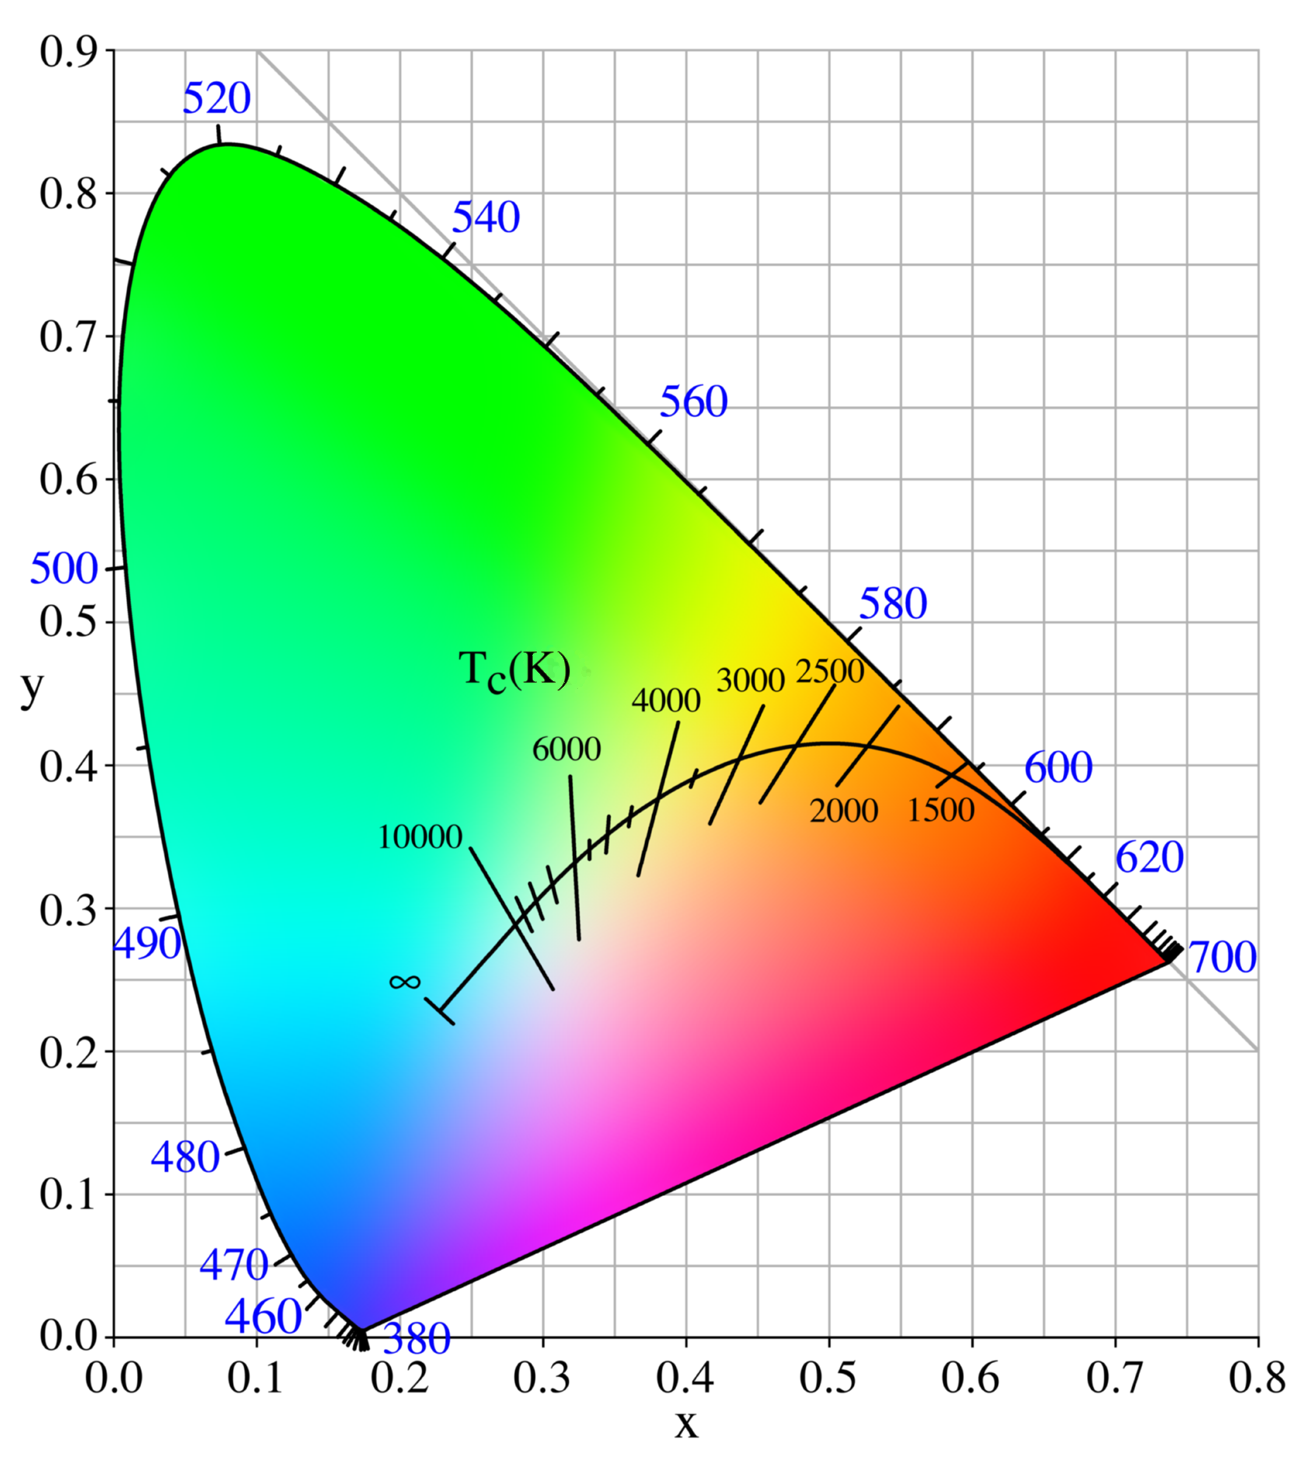
\includegraphics{figures/metaphor/PlanckianLocus}}
\caption{The Planckian Locus in the CIE 1931 chromaticity diagram. Chromaticity refers only to the hue of a colour, without other domains such as saturation.}
\end{figure}
\end{example}

Abstractly, the Planckian Locus is a continuous function mapping the positive real line representing the conceptual domain of temperature into the plane representing the conceptual domain of colour. The Planckian locus is the basis of colourist-talk about colour schemes in terms of temperature, which allows them to coordinate movements in colourspace using the terminology of temperaturespace, e.g. \texttt{make this shot warmer}. This fits with what we would prototypically expect a metaphor to allow us to do with meanings.

However, the particular mathematical conception of metaphor-as-map in Example \ref{ex:planck1} is too rigid: it only goes one way. It is a specific and inflexible kind of metaphor that does not behave at all outside its specified boundaries. For example, colourists have to deal with offsets towards green and magenta, which are not in the chromaticity codomain of the function given by Planck's law. It would be truer to life if we further analysed the function as mediated by a strip.

\begin{example}[The colourist's Planckian Locus]
Now we aim to extend our mathematical model to accommodate the fact that colourists deal with chromatic offsets or deviations from the mathematically precise locus given by Planck's law.
\begin{figure}[h]
\centering
\scalebox{0.5}{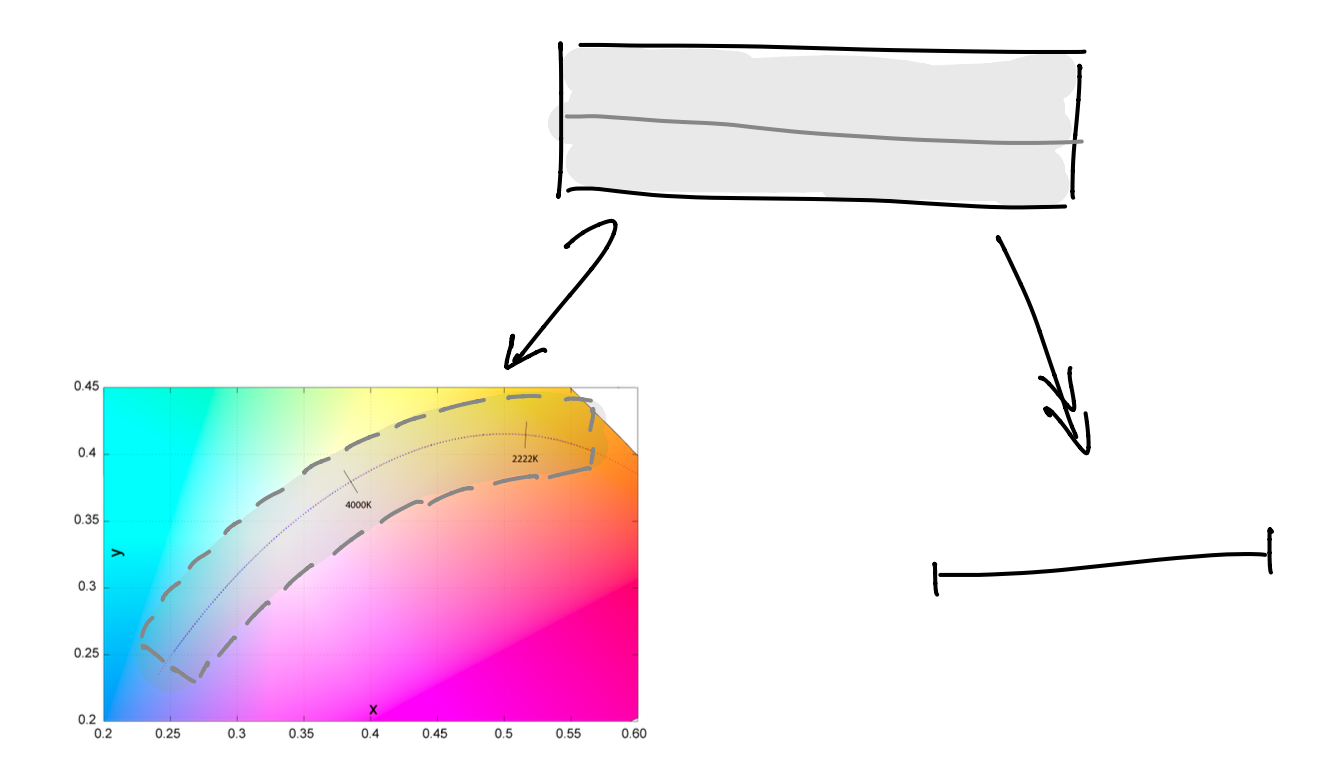
\includegraphics{figures/metaphor/colourlocus1}}
\caption{Consider the unit square (depicted as a strip) as a fiber bundle over the unit interval representing temperature range. There is an injective continuous map from the strip into colourspace that is centered on the Planck Locus.}
\end{figure}
\begin{figure}[h]
\centering
\scalebox{0.5}{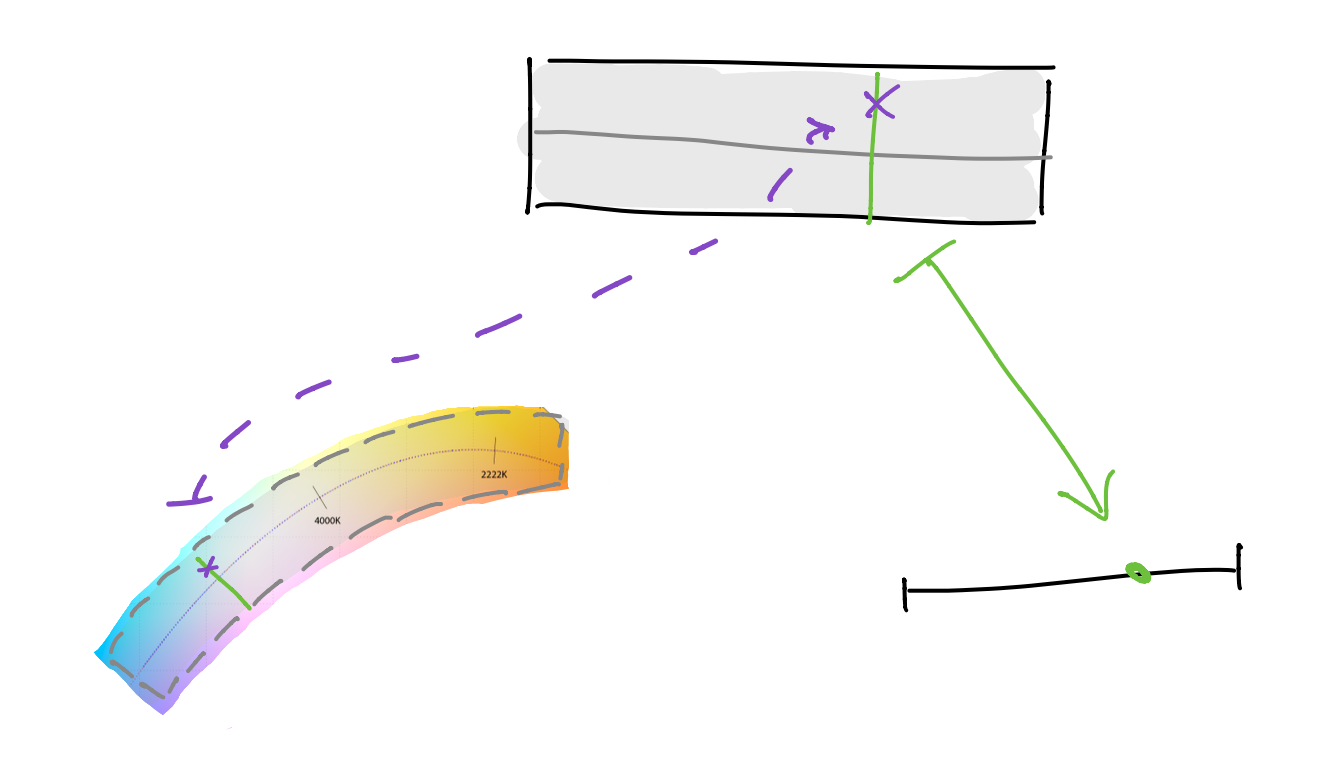
\includegraphics{figures/metaphor/colourlocus2}}
\caption{The left leg is bijective in the image restriction, so any point or displacement in the offset-strip in colourspace can be lifted to a point in the apex strip, which is then projected down along with other points in the vertical fiber to a point in temperaturespace. So we have a decategorified cofunctor!}
\end{figure}
\end{example}

A refinement we have just captured is the partially-structuring nature of metaphor \citep{lakoff_metaphors_2003}. In the language of our running example, pure green is outside the scope of the colour-temperature correspondence given by the Planckian Locus, so the metaphor is only a partial structuring of the colour domain according to the temperature domain. This partiality in the colour domain means that it would have been inappropriate to model the passage of colour-talk to temperature-talk as a function from colour to temperature, as functions are total, rather than partial, on their domain. While it is conceptually nice that we are on the way to recovering monoidal cofunctors as a model of metaphor, why didn't we stay simple and just use a partial function? The answer is that the strip at the apex represents the \emph{talk} part of colour- and temperature-talk.

\begin{example}[Conceptual transfer between domains]
When colourists use the temperature metaphor they might say "hot", "warm", "cooler", which are not specific temperature ranges in Kelvin, but concepts in temperature-space. Recalling that we may consider concepts to be open sets of a topology (and comparatives as opens of the product), we observe that we can linguistically model regions on the positive reals with words \texttt{little} (labelled $l$), \texttt{lot} (labelled $L$), and \texttt{more} (labelled $M$), an algebraic basis from which derive \texttt{less} by symmetry, and other regions such as \texttt{more than a little, less than a lot}. In this particular running example, it happens that both legs of the span of functors have a lifting property, which explains how we might model the fact that conceptual colourist-talk of "daylight" or "candlelight" in the colour domain can be sensibly interpreted in the temperature domain. The formalisation of this fact follows by symmetry from this example.
\begin{figure}[h]
\centering
\resizebox{0.8\textwidth}{!}{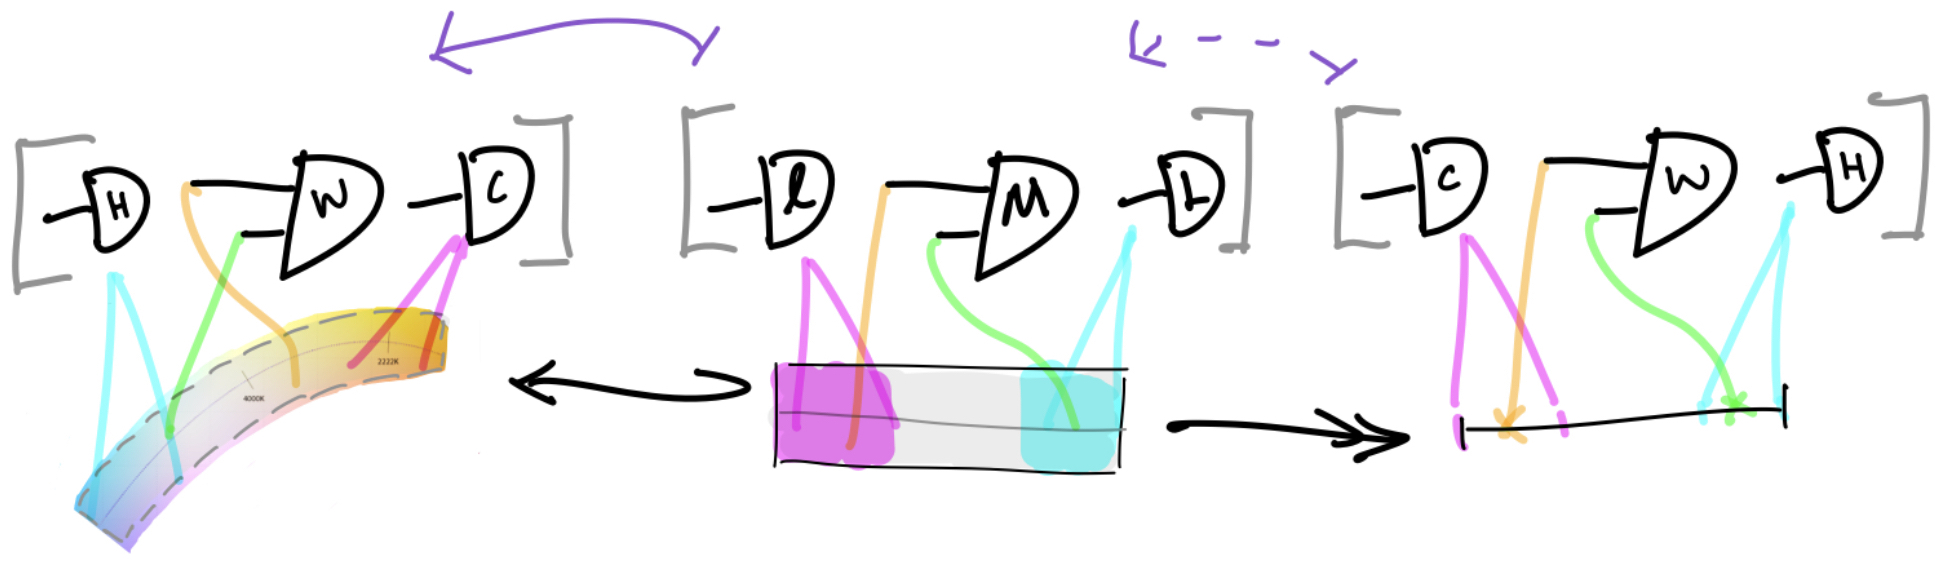
\includegraphics{figures/metaphor/offset1.jpeg}}
\caption{Starting from the right, the lifting property of the right leg is what lets us map "hotter and colder" temperature talk into the more abstract quantity-talk of "more and less" in the apex strip. Then the left functor sends quantity-talk into the colour domain, which allows "hotter and colder" to be used in the colour domain.}
\end{figure}
\begin{figure}[h]
\centering
\resizebox{0.8\textwidth}{!}{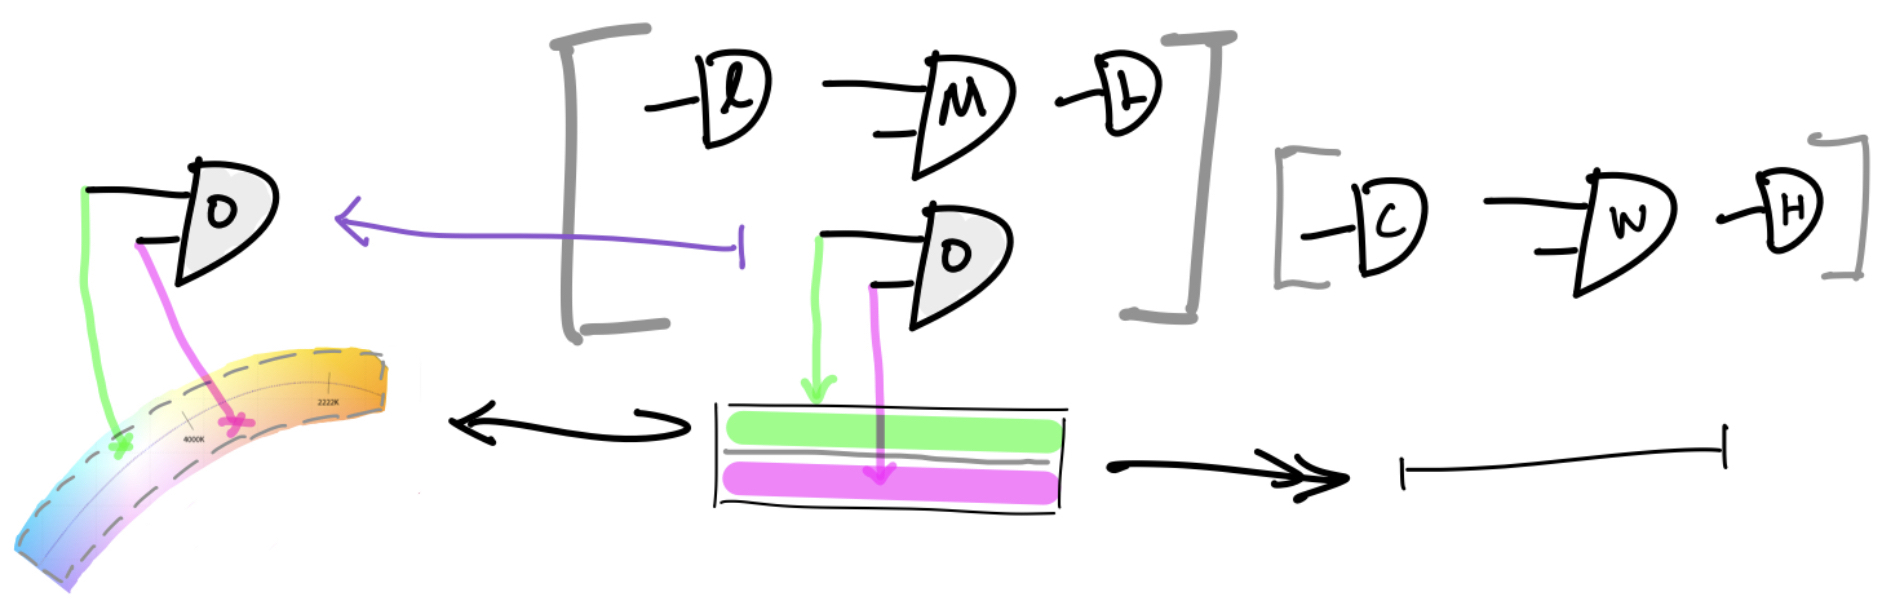
\includegraphics{figures/metaphor/offset2.jpeg}}
\caption{The additional expressive power that the apex strip gives is the concept of vertical offset, which doesn't appear in the real line. So the apex strip allows talk of quantity and offset, and this offset, when translated into the colour domain, allows talk of offset towards and away from, for instance, green.}
\end{figure}
\end{example}
\clearpage

\subsection{Time and Money: complex conceptual structure}

Metaphor is perhaps the only methodology we have for making sense of certain abstract concepts, such as Time. For example, many languages make use of the metaphor \texttt{TIME is SPACE}, in which space-talk is used to structure time. In English, the future is ahead of us and the past behind, while conversely, for the Aymara the future is behind and the past is ahead. Orthogonally, in Mandarin the future is below and the past is above. We have already demonstrated that we have the tools to deal with conceptual transfer between static conceptual spaces viewed as topological spaces via spans of continuous maps. What is of concern to us are \emph{dynamic} metaphors that involve a conceptual space-\emph{time} with agents and capabilities and so on. The following discussion draws heavily from \citep{lakoff_metaphors_2003}.\\

For example, in English, we make ample use\footnote{To our detriment. We could just as well have chosen the metaphor \texttt{TIME is FOOD}, which provides a liberating sense of mastery (at least in a context where food is abundant): time can be prepared, produced, consumed, spiced if dull and best shared with loved ones.} of the metaphor \texttt{TIME is MONEY}. There two mathematically relevant aspects of metaphor that I want to draw attention to for this metaphor. Firstly, that the conceptual affordances money-talk is marshalled to give structure to time-talk, where there is no such structure were it not for the metaphor. Secondly, that metaphor has a partial nature, in that it is not the case that the metaphor licenses all kinds of money-talk to structure time-talk.\\

To establish the first point of conceptual transfer, a phrase like \texttt{Do you have time to look at this?} is completely sensible to us, but literally meaningless; even if we had an oracle to measure possession, what would we point it at to measure a person's possession of time? Even if we accept some argument that the concept of possession is innate to the human faculty, when we say \texttt{This is definitely worth your time!} or \texttt{What a waste of time.}, we are drawing upon value-talk that is properly contingent in the socially constructed sense upon the conceptual complex of money.\\

To establish the second point of partiality, consider that money can be stored in a bank, whereas there is no real corresponding thing in the common conceptual vocabulary which one can store time and withdraw it for later use\footnote{Although, in a wonderful example of `pataphysical thinking, "Time Banks" have existed since the 19th century, which are practices of reciprocal service exchange that use units of time as currency.}. But the partiality constraint is itself partial. For instance, one can invest money into an enterprise in the expectation of greater returns, and this is not appropriate for many domains of time-talk, but there is a metaphorical match in some specific contexts, such as text-editor-talk: \texttt{learning vim slows you down at first but it will save you time later}.\\

Now I'll try to demonstrate by example that the kinda-cofunctors we explored in Section \ref{sec:miracle} between text circuits do all of the things we have asked for. The components of text circuits serve as an algebraic basis for dynamic conceptual complexes, while the kinda-cofunctor handles partial structuring of one conceptual domain in terms of another.

\begin{example}[\texttt{Vincent spends his morning writing}]
To begin a formal figurative interpretation via the metaphor \texttt{TIME is MONEY}, we require some model of the conceptual domain of money, as well as a topological interpretation. As a first pass, we understand that money can be exchanged for goods and services, so we will settle for a text-circuit signature for trade to serve as the conceptual domain as the apex of a cofunctor, given in Figure \ref{fig:tradesig}. The elements of the topological model are given in Figure \ref{fig:topmodel}. The behaviour of the opfibration part of the cofunctor is detailed in Figure \ref{fig:fibroles}, and that of the identity-on-objects functor in Figures \ref{fig:interpret}, \ref{fig:time0}, and \ref{fig:time1}. The figurative model serves as a foundation from which truth-theoretical semantics can begin. In the sketched interpretation, there aren't too many interesting questions one can ask, but the purpose of this example is to point out that in principle, we can exploit the systematicity of metaphor by constructing figurative mechanical models for which interesting questions can be asked and answered truth-theoretically, as in Figure \ref{fig:fullermodel}.
\begin{figure}[h]\label{fig:tradesig}
\centering
\resizebox{\textwidth}{!}{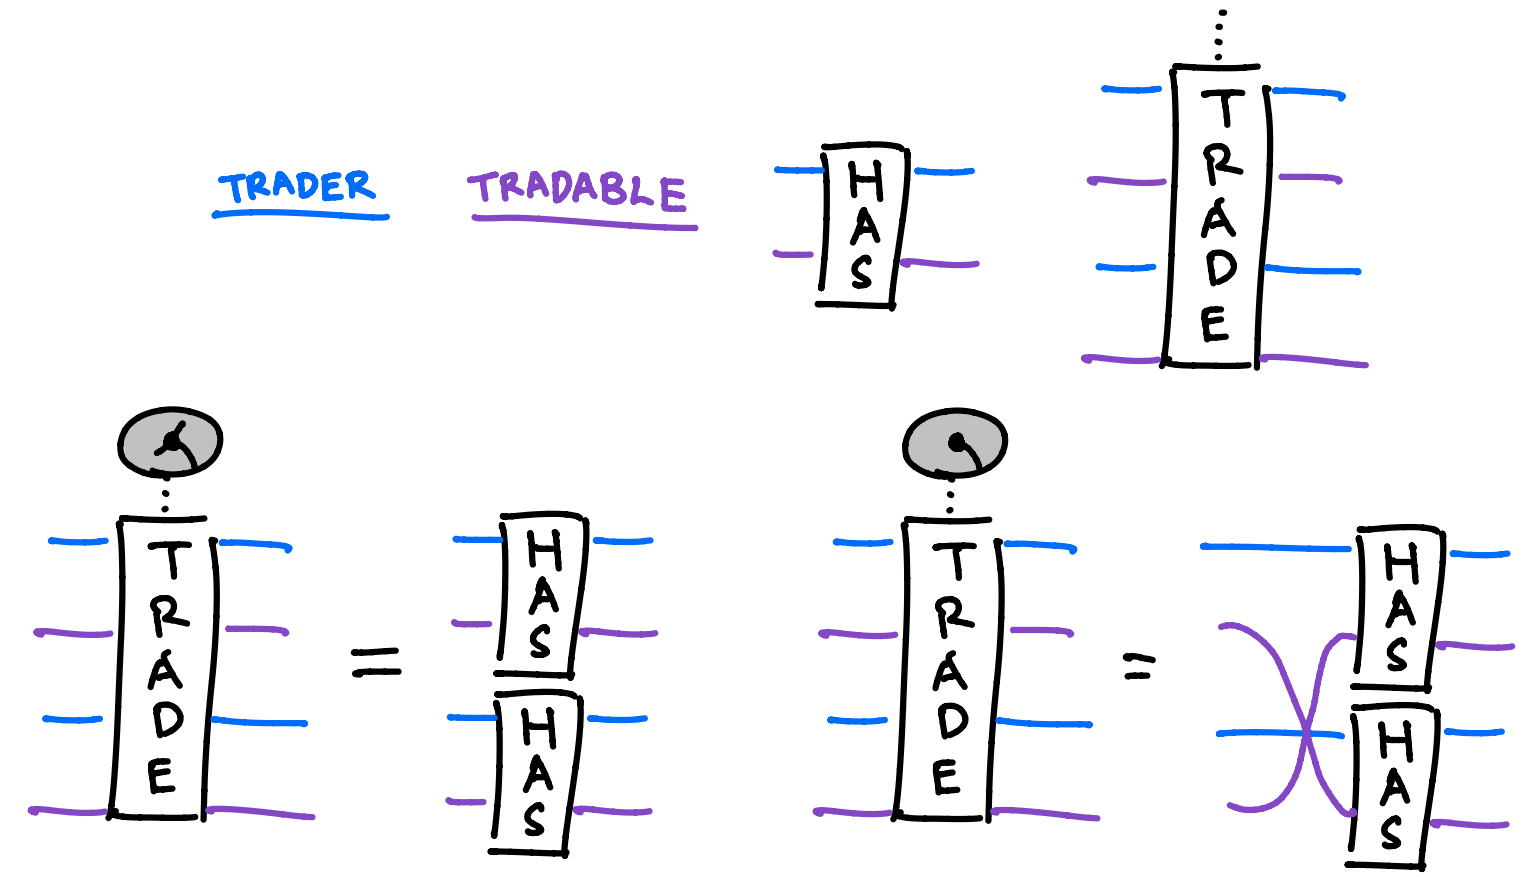
\includegraphics{figures/metaphor/tradesignature}}
\caption{In the \texttt{TRADE} signature, we define two roles as wires: \texttt{TRADERS} and \texttt{TRADEABLES}. There is one static relation \texttt{HAS} to indicate a trader's ownership of a tradeable, which can be further elaborated with equations to indicate e.g. exclusivity of ownership by interpreting violations of exclusivity as a zero morphism, assumed but elided for brevity. There is one dynamic verb (treated as a homotopy) \texttt{TRADE}, which at time 0 enforces a precondition that the traders have their respective tradables, and at time 1 (completion of the trade), the traders swap possession of their tradeables. The \texttt{TRADE} signature contains all nominal instantiations of nouns with respect to roles, which will be illustrated shortly.}
\end{figure}
\begin{figure}[h]\label{fig:topmodel}
\centering
\resizebox{0.75\textwidth}{!}{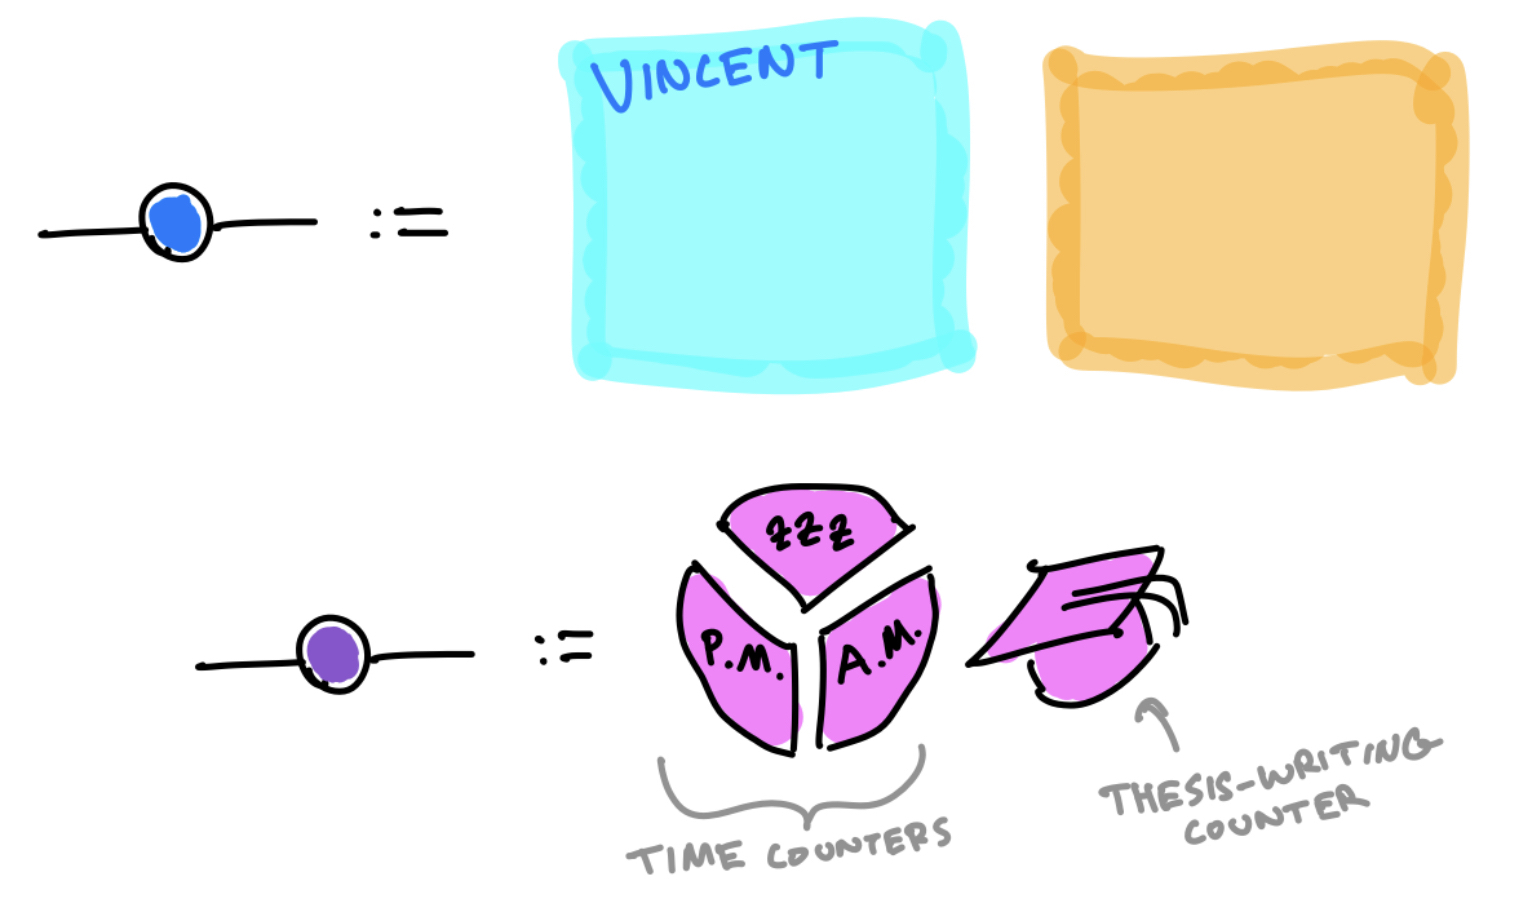
\includegraphics{figures/metaphor/toptrademodel.jpeg}}
\caption{We build the topological model from two sticky spiders in the Euclidean plane. The \texttt{TRADER} spider will distinguish two regions of possession, so that \texttt{HAS} may be interpreted as a region-test. The \texttt{TRADEABLES} spider will specify four meeples or counters, three for time, and one for thesiswriting; we will use the configuration space of the \texttt{TRADEABLES} spider to regulate their movement and distribution.}
\end{figure}
\begin{figure}\label{fig:fibroles}
\centering
\resizebox{\textwidth}{!}{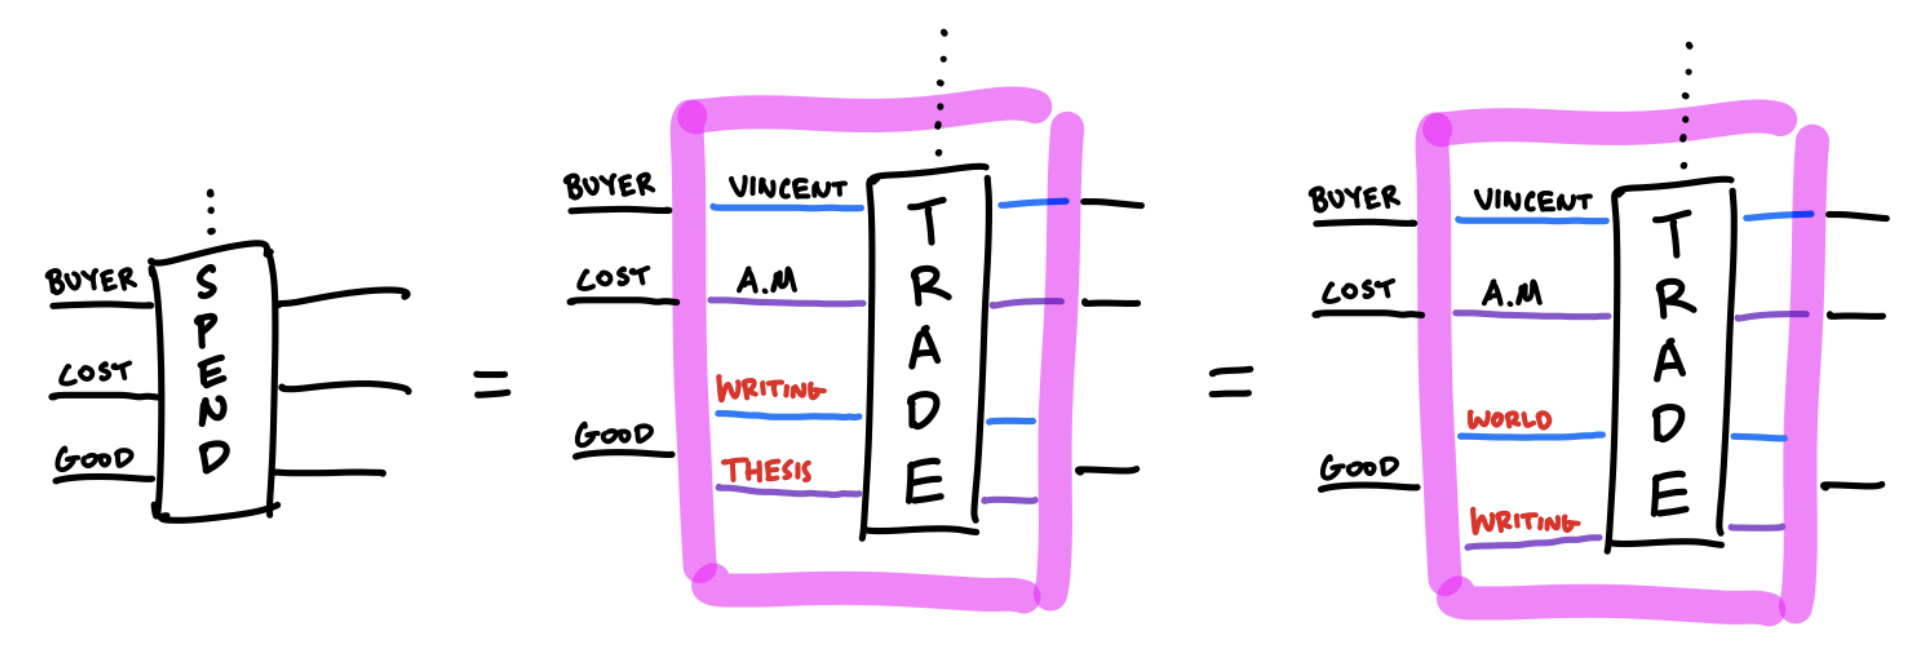
\includegraphics{figures/metaphor/fibroles}}
\caption[-10cm]{Next, we have to specify what the discrete opfibration is doing. Recalling our functor box notation, we can consider the job of the discrete opfibration to be role assignment from the verb \texttt{SPEND} in the utterance to the verb \texttt{TRADE} in the conceptual domain. The opfibration forgets about role-assignments in its domain by sending them to the monoidal unit. The lift of the opfibration is a role-assignment. (Arguably) unambiguously in this example, \texttt{Vincent} is the spender and the first trader, and \texttt{A.M} is the cost and the first tradeable. However, there are two options to resolve \texttt{writing} treated as a noun-phrase in the role of \texttt{GOOD}. In the first lift, \texttt{writing} is resolved as the other trader, and the implicit good as \texttt{thesis}. In the second lift, \texttt{writing} is the tradeable and something else is the trading counterparty, such as \texttt{the world}.}
\end{figure}
\begin{figure}[h]\label{fig:interpret}
\centering
\resizebox{0.5\textwidth}{!}{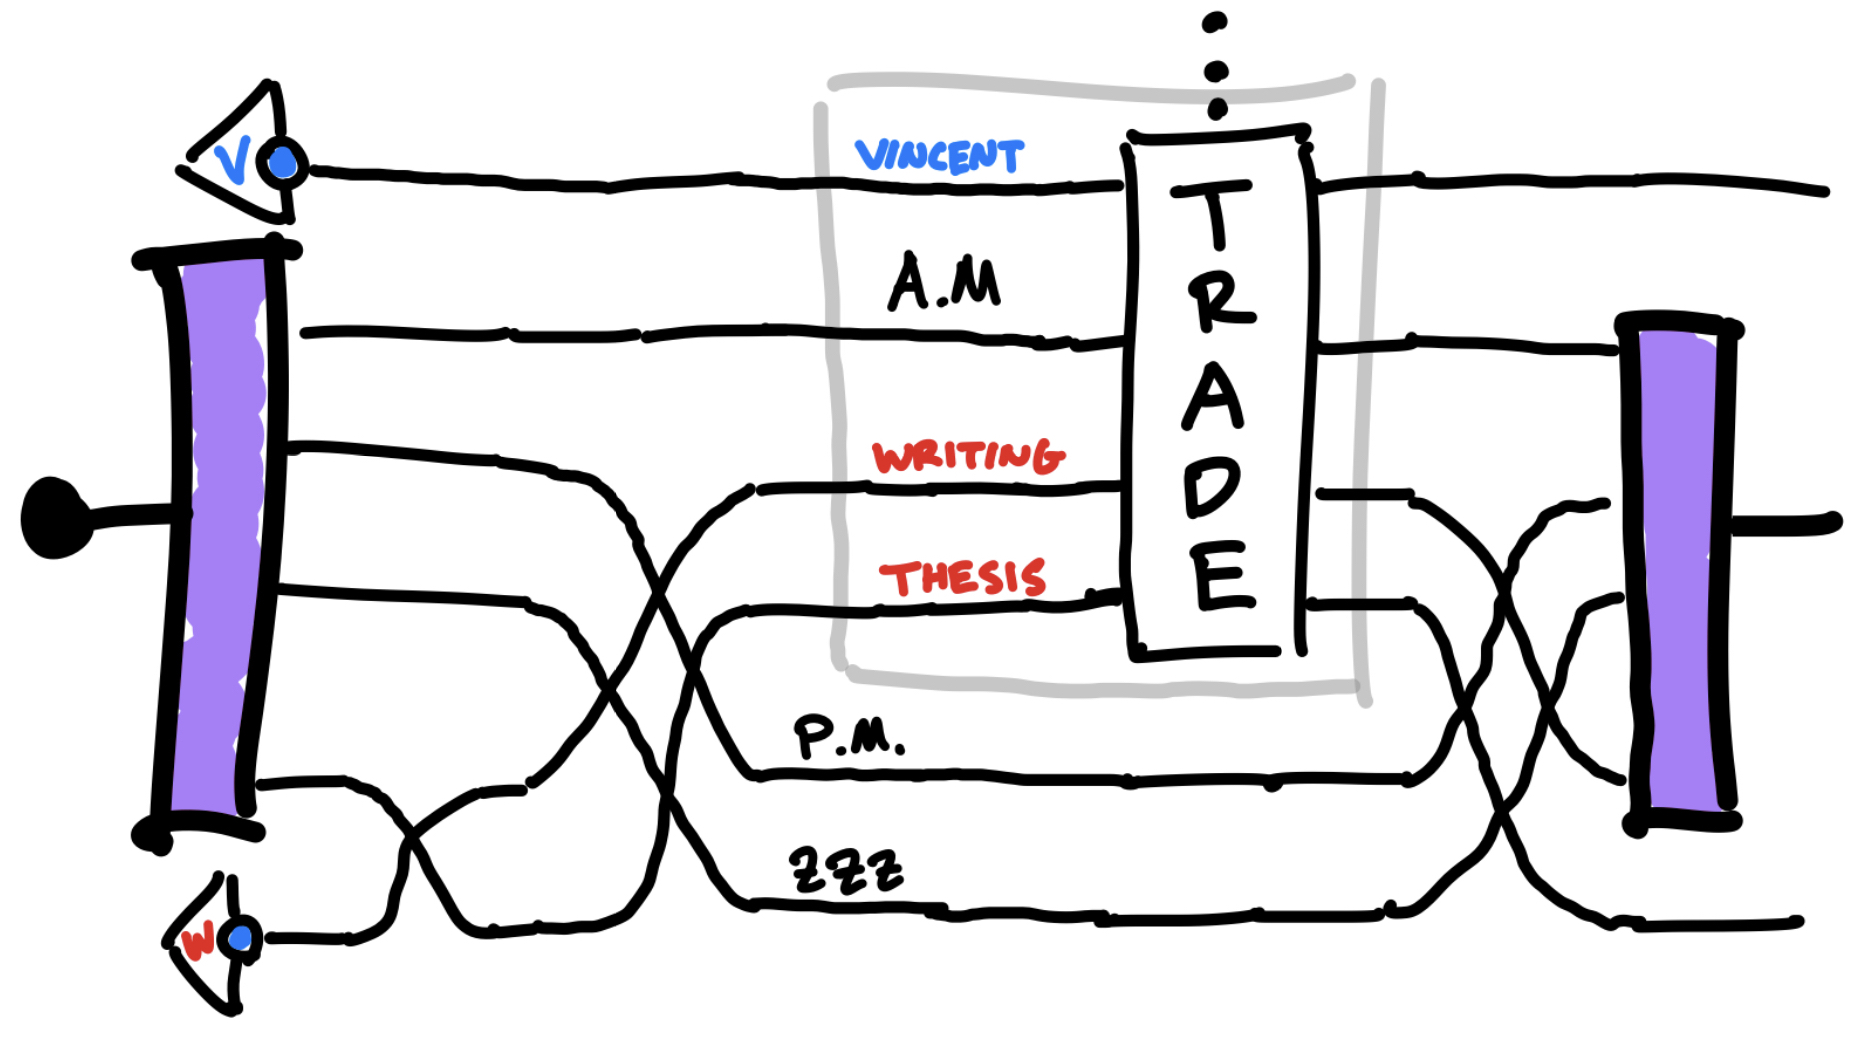
\includegraphics{figures/metaphor/interpret.jpeg}}
\caption{The section of the opfibration over the \texttt{SPEND} verb is a tabulation of all the ways in which conceptual roles in the \texttt{TRADING} domain can be assigned. To continue the example, we will assume the first lift in Example \ref{fig:fibroles} as our interpretation. The identity-on-objects functor part of the cofunctor maps our chosen interpretation into the following diagram in \textbf{ContRel}. The configuration space of the \texttt{TRADEABLES} spider is expanded via split idempotent so that all thin wires in the diagram are typed as the Euclidean plane. Recalling Example \ref{ex:chessboard}, \texttt{HAS} is interpreted as the intersection of the position of a counter with the possessive region of the respective trader.}
\end{figure}
\begin{figure}[h]\label{fig:time0}
\centering
\resizebox{\textwidth}{!}{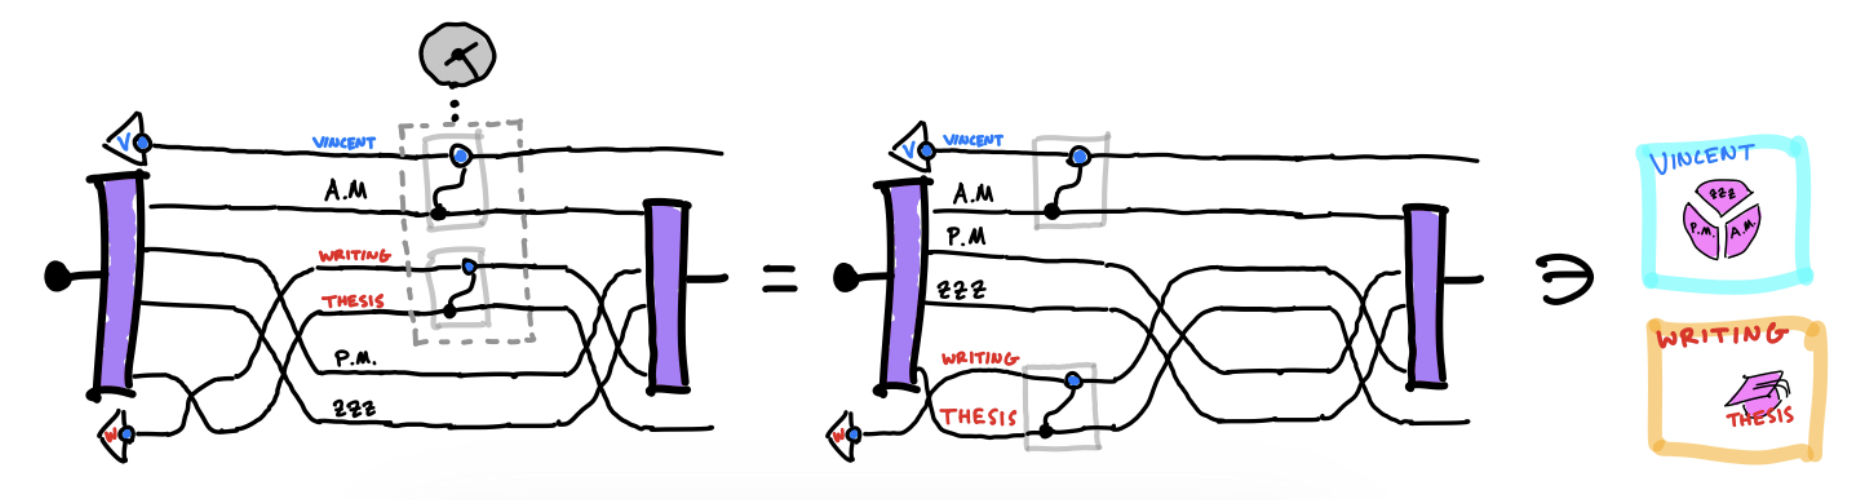
\includegraphics{figures/metaphor/time0.jpeg}}
\vspace{5cm}
\caption{We may verify that the equations governing \texttt{TRADE} cohere with our topological figures. At time 0, before the trade, we can calculate that the permissible figures have \texttt{Vincent} in possession of \texttt{A.M} and \texttt{writing} in possession of \texttt{thesis}.}
\end{figure}
\begin{figure}[h]\label{fig:time1}
\centering
\resizebox{\textwidth}{!}{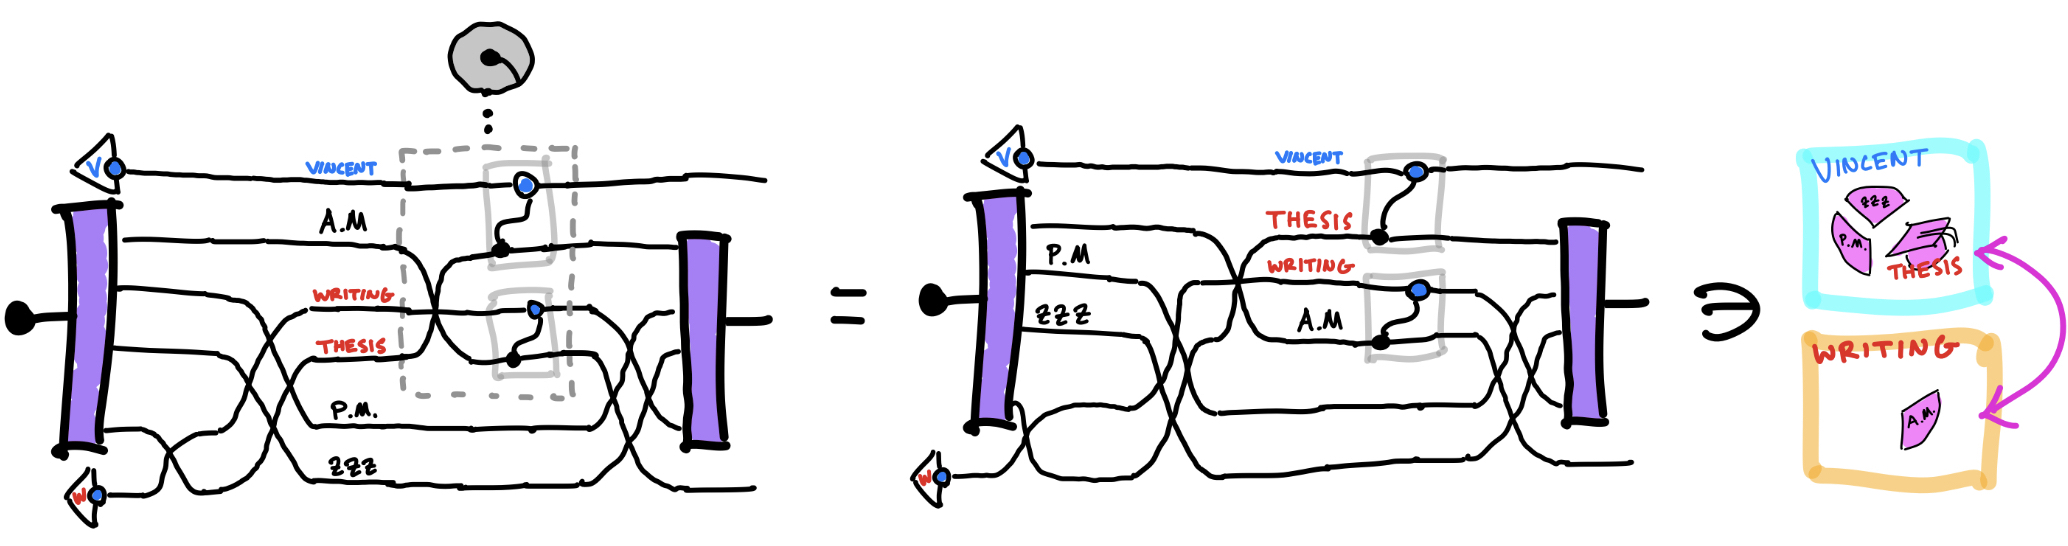
\includegraphics{figures/metaphor/time1.jpeg}}
\caption{At time 1, we may calculate that the permissible figures must be such that \texttt{Vincent} is in possession of \texttt{thesis} and \texttt{writing} is in possession of what was previously my morning.}
\end{figure}
\begin{figure}[h]\label{fig:fullermodel}
\centering
\resizebox{\textwidth}{!}{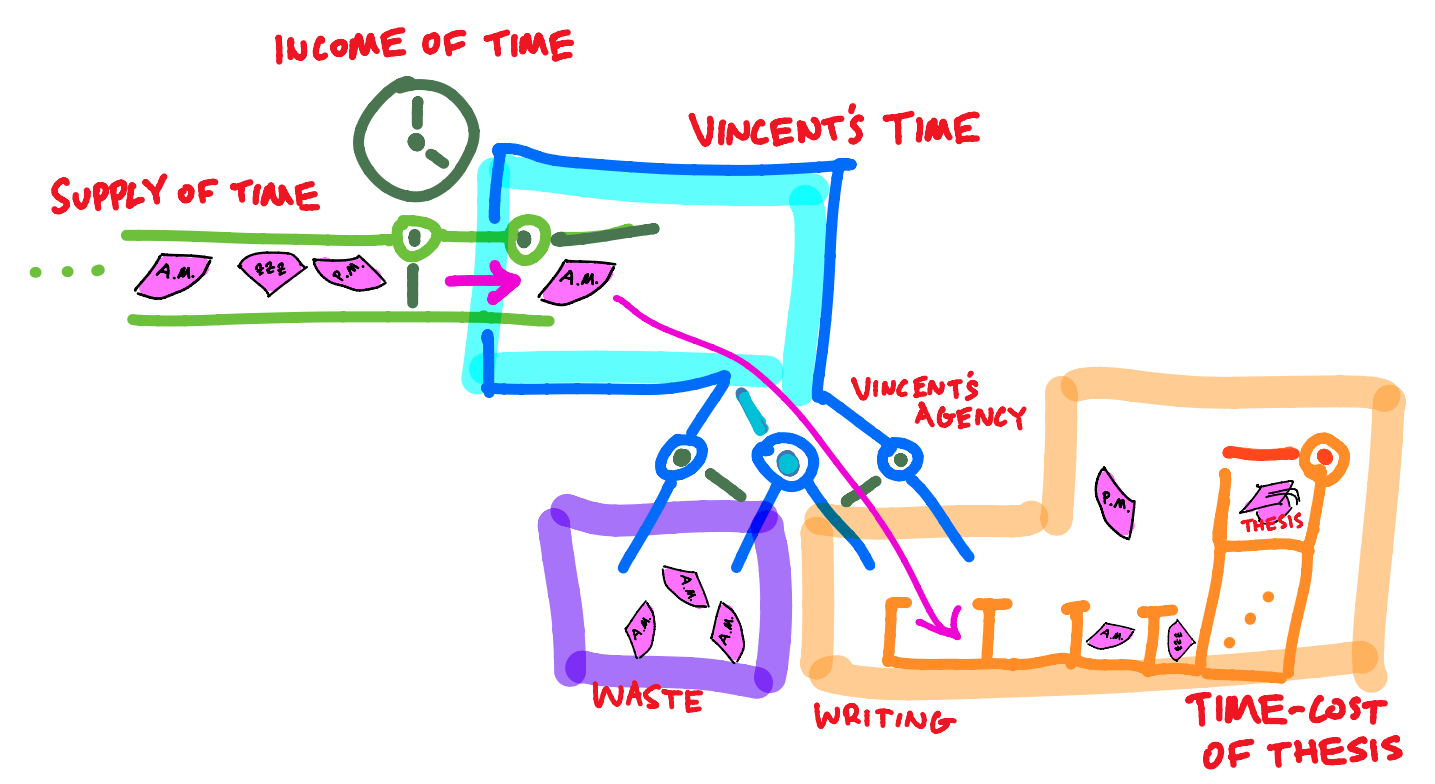
\includegraphics{figures/metaphor/fullermodel}}
\caption{In a more detailed conceptual model of \texttt{TIME is MONEY}, rather than just \texttt{TRADE}, we might consider income, the spender's agency, and cost. In Euclidean 3-space, we might model income as a clock-gated mechanism that deposits time-tokens serially into Vincent's possession, along with his agency as a gated chute, and the time cost of writing a thesis as a dispenser that requires a certain number of tokens to release a thesis-token into Vincent's possession. In this sketch model, one obtains short films for \texttt{He used to waste his mornings but now he spends them writing}, or \texttt{He once spent an evening writing but made no progress}. One can then ascertain certain consequences truth-theoretically; for instance that there is at least one morning that was not spent on writing, or that there is at least one evening spent on writing but not inside the slot that would help a thesis-release mechanism trigger. In every case, cofunctoriality handles bookkeeping for role-interpretation choices and guarantees systematicity of the topological figure according to the signature at the apex model that models the organising concept.}
\end{figure}
\end{example}

\clearpage

\clearpage
\newpage

\newthought{\textbf{Objection:} Hold on, that last figure wasn't justified.} It's justified in principle.

\newthought{\textbf{Objection:} On what principles?} Good question!

\section{The logical conclusions}

Like how the Church-Turing thesis is a declaration of the limits of computability by informed consensus, we might ask what idealised theses we might posit. Now we recap what we've seen.

\newthought{Review of Chapter 1.} We demonstrated that by encoding meaning-relations as topological connectivity (which is in a broad sense the whole point of string diagrams as a bridge between algebra and topology), we can capture systematic structural relationships as configurations of functors. In particular, we were able to diagrammatically reason about the correspondence between a pair of simple productive and parsing grammars subject to the evident constraints of communication. With some imagination, there are two theses here to obtain, or declare:

\begin{thesis}[String diagrams for composition]
Compositionality equals topological representability; in particular, meaning relations in text are witnessed by connectivity of string diagrams.
\end{thesis}

\begin{thesis}[String diagrams for systematic relationships]
Systematicity equals functorially witnessed relations; in particular, spans of functors between families of string diagrams witness agreement between different theories as topological equivalence.
\end{thesis}

\newthought{Review of Chapter 2.} We demonstrated that from the  mathematical perspective of weak $n$-categories, there is no fundamental difference between a broad class of productive grammars at a structural level, including all string-rewrite systems, tree-adjoining grammars, and transformational grammars. In this setting, we created a circuit-growing grammar and demonstrated a correspondence -- the Text Circuit Theorem -- between text circuits and grammatical text for a fragment of English, hence justifying the na\"{i}ve composition of text circuits as a generative grammar. We moreover indicated how the correspondence could be expanded to cover larger fragments of English, and indicated how the particular form of text circuits made them preferable for practical application. We also mentioned that in some sense the correspondence wasn't important from the perspective that text circuits were algebraic jazz for text. Putting together the views from Chapters 0, 1 and 2, productive grammars are just ways of generating topological data, and the only practically interesting constraint about whether a productive grammar is suitable for natural language stems from whether it is paired with a parsing grammar that systematically agrees on semantics up to topological equivalence -- i.e. precisely the kind of equivalence that string diagrams are invariant under. So we might reach for:

\begin{thesis}[String diagrams for syntax]
Syntax equals a coherent method of synthesising \emph{and} analysing composition; in particular, any internally consistent conception of natural language syntax in terms of string diagrams is permissible.
\end{thesis}

\newthought{Review of Chapter 3.} We give content to string diagrams by interpreting them in the category of continuous relations \textbf{ContRel}. We string-diagrammatically characterised labelled collections of disjoint shapes, along with processes that allowed us to puppeteer them in space, and test for topological relationships between shapes and places such as containment and touching. In particular, since we defined rigid motions and spatial-exclusivity of shapes, we have covered enough to linguistically specify any mechanical model up to topological invariance, and it is no difficulty to see how this setting may be expanded to include distances, directions, and forces. We saw how \textbf{ContRel} naturally gives voice to the structure of text circuits as higher-order modifications, and we also saw how \textbf{ContRel} permits us to model simple intensions via containers that mirror the space around them, which also yields a novel mathematical model of \textbf{FinRel} equipped with a Turing object, which is a mathematical model for universal computation and, in the linguistic setting, syntactic polymorphism. On the faith that any consistent and interesting system of string diagrams has some consistent and interesting computational reification, we might integrate the views of the previous chapters to obtain:

\begin{thesis}[String diagrams for semantics]
Semantics equals computatation; in particular, any consistent computational interpretation of the content of string diagrams is permissible.
\end{thesis}

\subsection{How things could be.}

\begin{thesis}[String diagrams for text]
String diagrams suffice for formal linguistics.
\end{thesis}

That's the best-case scenario if we accept all of the best-case scenarios above. What would such a hypothetical world look like? Recall that I still owe a worked example of computing a metaphor. Sadly, I think in a best-case hypothetical world, working out the conduit metaphor would be a kind of dull problem sheet for undergraduate mathematical linguists, who may well ask "what's the point?". Indeed, what is the point of learning all of this mathematically complicated machinery to do something everyone can do effortlessly? I'm not sure of the answer, but I do know that turning language into pictures by turning language into pictures was good fun.

\newpage

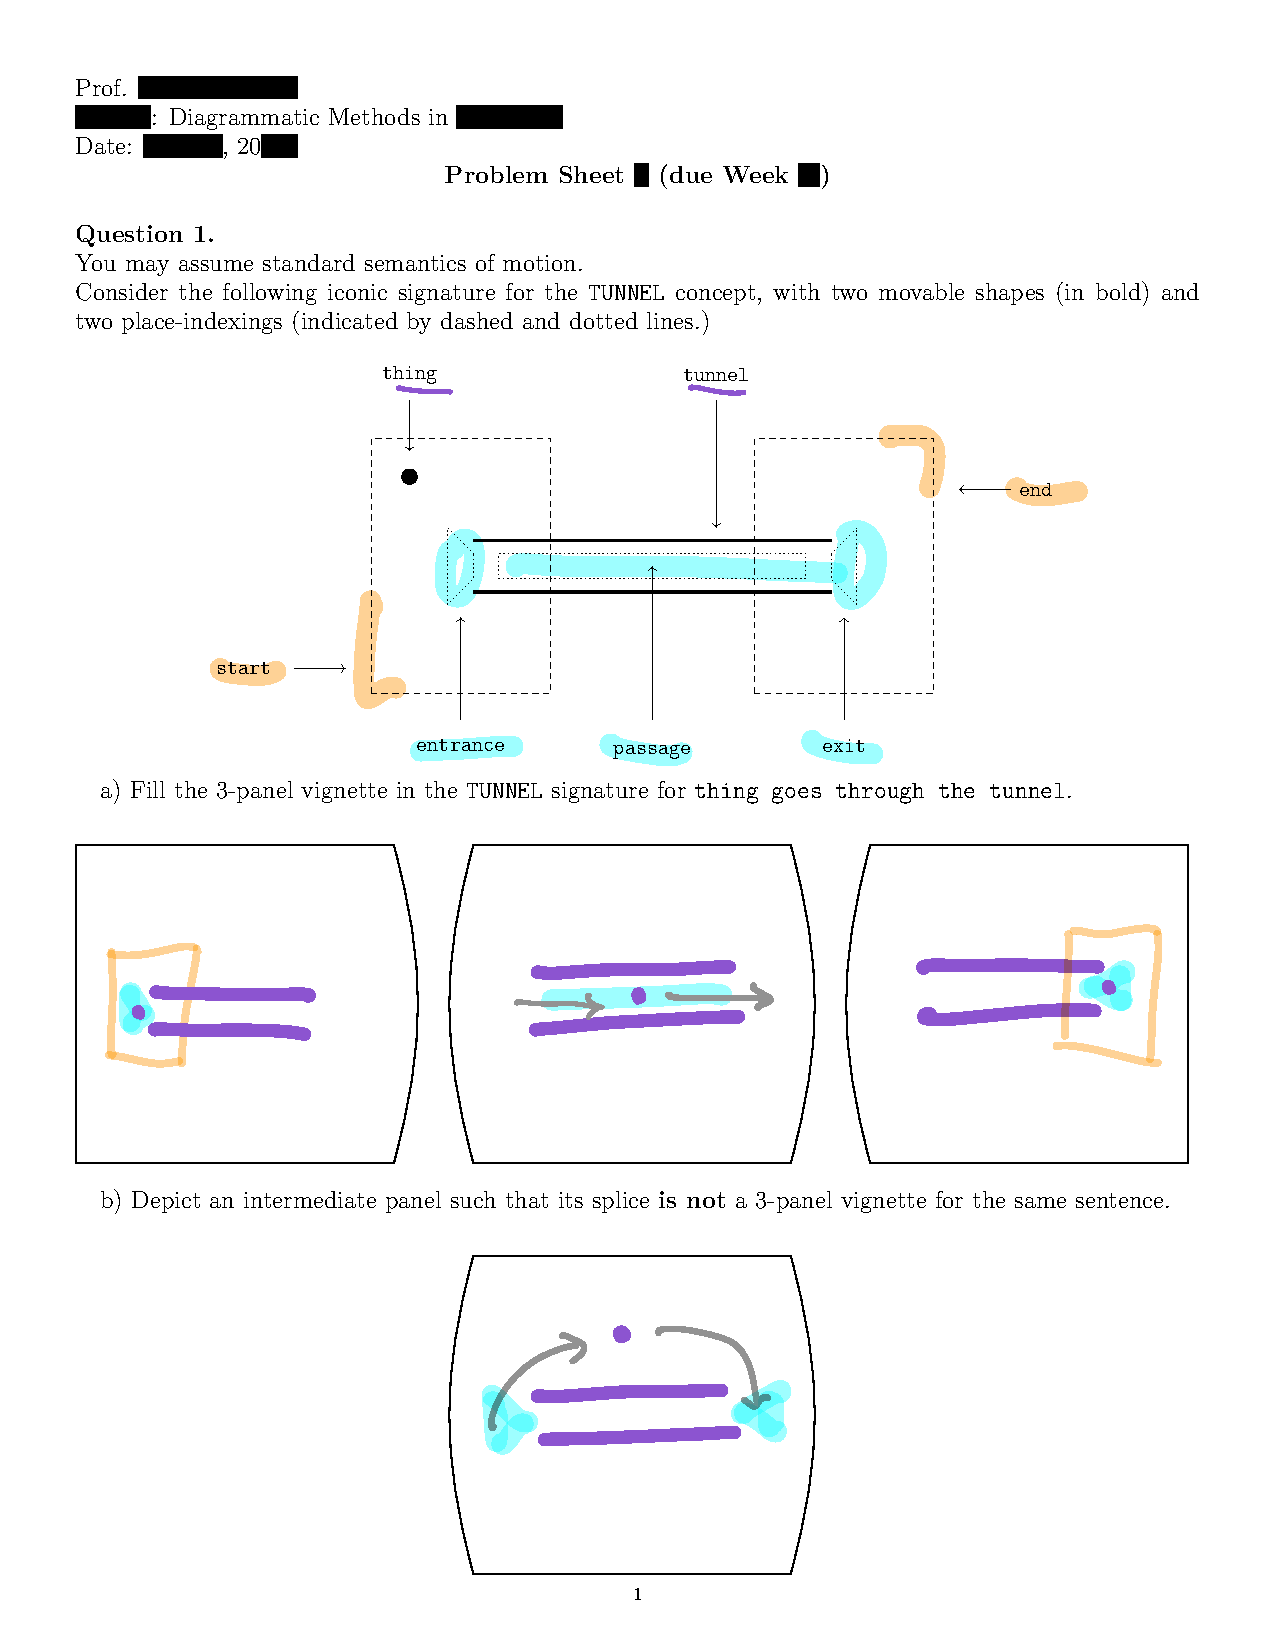
\includepdf[angle=90,pages=-]{metaphorproblemsheet-filled}
\clearpage






\end{document}